% Options for packages loaded elsewhere
\PassOptionsToPackage{unicode}{hyperref}
\PassOptionsToPackage{hyphens}{url}
\PassOptionsToPackage{dvipsnames,svgnames,x11names}{xcolor}
%
\documentclass[
  letterpaper,
  DIV=11,
  numbers=noendperiod]{scrreprt}

\usepackage{amsmath,amssymb}
\usepackage{iftex}
\ifPDFTeX
  \usepackage[T1]{fontenc}
  \usepackage[utf8]{inputenc}
  \usepackage{textcomp} % provide euro and other symbols
\else % if luatex or xetex
  \usepackage{unicode-math}
  \defaultfontfeatures{Scale=MatchLowercase}
  \defaultfontfeatures[\rmfamily]{Ligatures=TeX,Scale=1}
\fi
\usepackage{lmodern}
\ifPDFTeX\else  
    % xetex/luatex font selection
\fi
% Use upquote if available, for straight quotes in verbatim environments
\IfFileExists{upquote.sty}{\usepackage{upquote}}{}
\IfFileExists{microtype.sty}{% use microtype if available
  \usepackage[]{microtype}
  \UseMicrotypeSet[protrusion]{basicmath} % disable protrusion for tt fonts
}{}
\makeatletter
\@ifundefined{KOMAClassName}{% if non-KOMA class
  \IfFileExists{parskip.sty}{%
    \usepackage{parskip}
  }{% else
    \setlength{\parindent}{0pt}
    \setlength{\parskip}{6pt plus 2pt minus 1pt}}
}{% if KOMA class
  \KOMAoptions{parskip=half}}
\makeatother
\usepackage{xcolor}
\setlength{\emergencystretch}{3em} % prevent overfull lines
\setcounter{secnumdepth}{5}
% Make \paragraph and \subparagraph free-standing
\ifx\paragraph\undefined\else
  \let\oldparagraph\paragraph
  \renewcommand{\paragraph}[1]{\oldparagraph{#1}\mbox{}}
\fi
\ifx\subparagraph\undefined\else
  \let\oldsubparagraph\subparagraph
  \renewcommand{\subparagraph}[1]{\oldsubparagraph{#1}\mbox{}}
\fi

\usepackage{color}
\usepackage{fancyvrb}
\newcommand{\VerbBar}{|}
\newcommand{\VERB}{\Verb[commandchars=\\\{\}]}
\DefineVerbatimEnvironment{Highlighting}{Verbatim}{commandchars=\\\{\}}
% Add ',fontsize=\small' for more characters per line
\usepackage{framed}
\definecolor{shadecolor}{RGB}{241,243,245}
\newenvironment{Shaded}{\begin{snugshade}}{\end{snugshade}}
\newcommand{\AlertTok}[1]{\textcolor[rgb]{0.68,0.00,0.00}{#1}}
\newcommand{\AnnotationTok}[1]{\textcolor[rgb]{0.37,0.37,0.37}{#1}}
\newcommand{\AttributeTok}[1]{\textcolor[rgb]{0.40,0.45,0.13}{#1}}
\newcommand{\BaseNTok}[1]{\textcolor[rgb]{0.68,0.00,0.00}{#1}}
\newcommand{\BuiltInTok}[1]{\textcolor[rgb]{0.00,0.23,0.31}{#1}}
\newcommand{\CharTok}[1]{\textcolor[rgb]{0.13,0.47,0.30}{#1}}
\newcommand{\CommentTok}[1]{\textcolor[rgb]{0.37,0.37,0.37}{#1}}
\newcommand{\CommentVarTok}[1]{\textcolor[rgb]{0.37,0.37,0.37}{\textit{#1}}}
\newcommand{\ConstantTok}[1]{\textcolor[rgb]{0.56,0.35,0.01}{#1}}
\newcommand{\ControlFlowTok}[1]{\textcolor[rgb]{0.00,0.23,0.31}{#1}}
\newcommand{\DataTypeTok}[1]{\textcolor[rgb]{0.68,0.00,0.00}{#1}}
\newcommand{\DecValTok}[1]{\textcolor[rgb]{0.68,0.00,0.00}{#1}}
\newcommand{\DocumentationTok}[1]{\textcolor[rgb]{0.37,0.37,0.37}{\textit{#1}}}
\newcommand{\ErrorTok}[1]{\textcolor[rgb]{0.68,0.00,0.00}{#1}}
\newcommand{\ExtensionTok}[1]{\textcolor[rgb]{0.00,0.23,0.31}{#1}}
\newcommand{\FloatTok}[1]{\textcolor[rgb]{0.68,0.00,0.00}{#1}}
\newcommand{\FunctionTok}[1]{\textcolor[rgb]{0.28,0.35,0.67}{#1}}
\newcommand{\ImportTok}[1]{\textcolor[rgb]{0.00,0.46,0.62}{#1}}
\newcommand{\InformationTok}[1]{\textcolor[rgb]{0.37,0.37,0.37}{#1}}
\newcommand{\KeywordTok}[1]{\textcolor[rgb]{0.00,0.23,0.31}{#1}}
\newcommand{\NormalTok}[1]{\textcolor[rgb]{0.00,0.23,0.31}{#1}}
\newcommand{\OperatorTok}[1]{\textcolor[rgb]{0.37,0.37,0.37}{#1}}
\newcommand{\OtherTok}[1]{\textcolor[rgb]{0.00,0.23,0.31}{#1}}
\newcommand{\PreprocessorTok}[1]{\textcolor[rgb]{0.68,0.00,0.00}{#1}}
\newcommand{\RegionMarkerTok}[1]{\textcolor[rgb]{0.00,0.23,0.31}{#1}}
\newcommand{\SpecialCharTok}[1]{\textcolor[rgb]{0.37,0.37,0.37}{#1}}
\newcommand{\SpecialStringTok}[1]{\textcolor[rgb]{0.13,0.47,0.30}{#1}}
\newcommand{\StringTok}[1]{\textcolor[rgb]{0.13,0.47,0.30}{#1}}
\newcommand{\VariableTok}[1]{\textcolor[rgb]{0.07,0.07,0.07}{#1}}
\newcommand{\VerbatimStringTok}[1]{\textcolor[rgb]{0.13,0.47,0.30}{#1}}
\newcommand{\WarningTok}[1]{\textcolor[rgb]{0.37,0.37,0.37}{\textit{#1}}}

\providecommand{\tightlist}{%
  \setlength{\itemsep}{0pt}\setlength{\parskip}{0pt}}\usepackage{longtable,booktabs,array}
\usepackage{calc} % for calculating minipage widths
% Correct order of tables after \paragraph or \subparagraph
\usepackage{etoolbox}
\makeatletter
\patchcmd\longtable{\par}{\if@noskipsec\mbox{}\fi\par}{}{}
\makeatother
% Allow footnotes in longtable head/foot
\IfFileExists{footnotehyper.sty}{\usepackage{footnotehyper}}{\usepackage{footnote}}
\makesavenoteenv{longtable}
\usepackage{graphicx}
\makeatletter
\def\maxwidth{\ifdim\Gin@nat@width>\linewidth\linewidth\else\Gin@nat@width\fi}
\def\maxheight{\ifdim\Gin@nat@height>\textheight\textheight\else\Gin@nat@height\fi}
\makeatother
% Scale images if necessary, so that they will not overflow the page
% margins by default, and it is still possible to overwrite the defaults
% using explicit options in \includegraphics[width, height, ...]{}
\setkeys{Gin}{width=\maxwidth,height=\maxheight,keepaspectratio}
% Set default figure placement to htbp
\makeatletter
\def\fps@figure{htbp}
\makeatother
\newlength{\cslhangindent}
\setlength{\cslhangindent}{1.5em}
\newlength{\csllabelwidth}
\setlength{\csllabelwidth}{3em}
\newlength{\cslentryspacingunit} % times entry-spacing
\setlength{\cslentryspacingunit}{\parskip}
\newenvironment{CSLReferences}[2] % #1 hanging-ident, #2 entry spacing
 {% don't indent paragraphs
  \setlength{\parindent}{0pt}
  % turn on hanging indent if param 1 is 1
  \ifodd #1
  \let\oldpar\par
  \def\par{\hangindent=\cslhangindent\oldpar}
  \fi
  % set entry spacing
  \setlength{\parskip}{#2\cslentryspacingunit}
 }%
 {}
\usepackage{calc}
\newcommand{\CSLBlock}[1]{#1\hfill\break}
\newcommand{\CSLLeftMargin}[1]{\parbox[t]{\csllabelwidth}{#1}}
\newcommand{\CSLRightInline}[1]{\parbox[t]{\linewidth - \csllabelwidth}{#1}\break}
\newcommand{\CSLIndent}[1]{\hspace{\cslhangindent}#1}

\usepackage{booktabs}
\usepackage{longtable}
\usepackage{array}
\usepackage{multirow}
\usepackage{wrapfig}
\usepackage{float}
\usepackage{colortbl}
\usepackage{pdflscape}
\usepackage{tabu}
\usepackage{threeparttable}
\usepackage{threeparttablex}
\usepackage[normalem]{ulem}
\usepackage{makecell}
\usepackage{xcolor}
\KOMAoption{captions}{tableheading}
\makeatletter
\@ifpackageloaded{tcolorbox}{}{\usepackage[skins,breakable]{tcolorbox}}
\@ifpackageloaded{fontawesome5}{}{\usepackage{fontawesome5}}
\definecolor{quarto-callout-color}{HTML}{909090}
\definecolor{quarto-callout-note-color}{HTML}{0758E5}
\definecolor{quarto-callout-important-color}{HTML}{CC1914}
\definecolor{quarto-callout-warning-color}{HTML}{EB9113}
\definecolor{quarto-callout-tip-color}{HTML}{00A047}
\definecolor{quarto-callout-caution-color}{HTML}{FC5300}
\definecolor{quarto-callout-color-frame}{HTML}{acacac}
\definecolor{quarto-callout-note-color-frame}{HTML}{4582ec}
\definecolor{quarto-callout-important-color-frame}{HTML}{d9534f}
\definecolor{quarto-callout-warning-color-frame}{HTML}{f0ad4e}
\definecolor{quarto-callout-tip-color-frame}{HTML}{02b875}
\definecolor{quarto-callout-caution-color-frame}{HTML}{fd7e14}
\makeatother
\makeatletter
\makeatother
\makeatletter
\@ifpackageloaded{bookmark}{}{\usepackage{bookmark}}
\makeatother
\makeatletter
\@ifpackageloaded{caption}{}{\usepackage{caption}}
\AtBeginDocument{%
\ifdefined\contentsname
  \renewcommand*\contentsname{Table of contents}
\else
  \newcommand\contentsname{Table of contents}
\fi
\ifdefined\listfigurename
  \renewcommand*\listfigurename{List of Figures}
\else
  \newcommand\listfigurename{List of Figures}
\fi
\ifdefined\listtablename
  \renewcommand*\listtablename{List of Tables}
\else
  \newcommand\listtablename{List of Tables}
\fi
\ifdefined\figurename
  \renewcommand*\figurename{Figure}
\else
  \newcommand\figurename{Figure}
\fi
\ifdefined\tablename
  \renewcommand*\tablename{Table}
\else
  \newcommand\tablename{Table}
\fi
}
\@ifpackageloaded{float}{}{\usepackage{float}}
\floatstyle{ruled}
\@ifundefined{c@chapter}{\newfloat{codelisting}{h}{lop}}{\newfloat{codelisting}{h}{lop}[chapter]}
\floatname{codelisting}{Listing}
\newcommand*\listoflistings{\listof{codelisting}{List of Listings}}
\makeatother
\makeatletter
\@ifpackageloaded{caption}{}{\usepackage{caption}}
\@ifpackageloaded{subcaption}{}{\usepackage{subcaption}}
\makeatother
\makeatletter
\@ifpackageloaded{tcolorbox}{}{\usepackage[skins,breakable]{tcolorbox}}
\makeatother
\makeatletter
\@ifundefined{shadecolor}{\definecolor{shadecolor}{rgb}{.97, .97, .97}}
\makeatother
\makeatletter
\makeatother
\makeatletter
\makeatother
\ifLuaTeX
  \usepackage{selnolig}  % disable illegal ligatures
\fi
\IfFileExists{bookmark.sty}{\usepackage{bookmark}}{\usepackage{hyperref}}
\IfFileExists{xurl.sty}{\usepackage{xurl}}{} % add URL line breaks if available
\urlstyle{same} % disable monospaced font for URLs
\hypersetup{
  pdftitle={Psychological data analysis for graduate students: PSYC401},
  pdfauthor={Rob Davies},
  colorlinks=true,
  linkcolor={blue},
  filecolor={Maroon},
  citecolor={Blue},
  urlcolor={Blue},
  pdfcreator={LaTeX via pandoc}}

\title{Psychological data analysis for graduate students:
\emph{PSYC401}}
\author{Rob Davies}
\date{2023-10-01}

\begin{document}
\maketitle
\ifdefined\Shaded\renewenvironment{Shaded}{\begin{tcolorbox}[sharp corners, frame hidden, enhanced, boxrule=0pt, interior hidden, breakable, borderline west={3pt}{0pt}{shadecolor}]}{\end{tcolorbox}}\fi

\renewcommand*\contentsname{Table of contents}
{
\hypersetup{linkcolor=}
\setcounter{tocdepth}{2}
\tableofcontents
}
\bookmarksetup{startatroot}

\hypertarget{preface-our-approach}{%
\chapter*{Preface: Our approach}\label{preface-our-approach}}
\addcontentsline{toc}{chapter}{Preface: Our approach}

\markboth{Preface: Our approach}{Preface: Our approach}

We can, here, explain a development in the approach we take in teaching
this course. Naturally, this development in approach will require a
parallel development in your approach to learning.

We are going to focus on working in research in context (see
Figure~\ref{fig-simple}).

\begin{figure}

{\centering 

\begin{figure}[H]

{\centering \includegraphics[width=5in,height=3.5in]{index_files/figure-latex/dot-figure-1.png}

}

\end{figure}

}

\caption{\label{fig-simple}Working in research in context.}

\end{figure}

You have been introduced to R. We know that some of you are new to R so
we will practice the skills you are learning. We will consolidate,
revise, and extend these skills.

We will encounter --- some, for the first time -- the linear model also
known as regression analysis. But the big change is this \emph{focus on
context}. The reason is that not talking about the context is risky for
how you approach, do, or think about data analysis.

In traditional methods teaching, the schedule of classes will progress
through a series of tests, one test a week, from simpler to more complex
tests. In this approach, the presentation is often brief about the
context: the question the researchers are investigating; the methods
they use to collect data; and, critically, the assumptions they make
about how your reasoning can get you from the things you measure to the
things you are trying to understand.

This approach is understandable but it presents a misleading view. It
implies that if you learn the method, and can match the textbook example
to your context then all you need to do is to apply the analysis code to
get the right result. This style of working is common, and it is often a
reasonable \emph{place to start}, but the isolation from context reduces
the application of judgment, and limits critical evaluation of
measurement, analysis assumptions, and sources of uncertainty.

\begin{tcolorbox}[enhanced jigsaw, opacitybacktitle=0.6, title=\textcolor{quarto-callout-tip-color}{\faLightbulb}\hspace{0.5em}{Tip}, arc=.35mm, colbacktitle=quarto-callout-tip-color!10!white, colframe=quarto-callout-tip-color-frame, leftrule=.75mm, opacityback=0, breakable, titlerule=0mm, left=2mm, bottomrule=.15mm, toprule=.15mm, colback=white, coltitle=black, bottomtitle=1mm, toptitle=1mm, rightrule=.15mm]

We can do better.

\end{tcolorbox}

A more productive approach -- this is the approach we will take -- is to
expose, and talk about some of the real challenges that anybody who
handles data, or quantitative evidence, deals with in professional life:

\begin{enumerate}
\def\labelenumi{\arabic{enumi}.}
\tightlist
\item
  Thinking about the mapping from our concerns to the research
  questions, to the things we measure, the analysis we do, and then the
  conclusions we make.
\item
  Selecting or constructing valid measures that can be assumed to
  measure the things they are supposed to measure.
\item
  Taking samples of observations, and making conclusions about the
  population.
\item
  Making estimates and linking these estimates to an account that is
  explicit about causes.
\end{enumerate}

\part{DATA ANALYSIS}

\bookmarksetup{startatroot}

\hypertarget{data-visualization}{%
\chapter{Data visualization}\label{data-visualization}}

\hypertarget{sec-aims}{%
\section{Aims}\label{sec-aims}}

In writing this chapter, I have two aims.

\begin{enumerate}
\def\labelenumi{\arabic{enumi}.}
\tightlist
\item
  The \textbf{first aim} for this chapter is to expose students to an
  outline summary of some key ideas and techniques for data
  visualization in psychological science.
\end{enumerate}

There is an extensive experimental and theoretical literature concerning
data visualization, what choices we can or should make, and how these
choices have more or less impact, in different circumstances or for
different audiences. Here, we can only give you a flavour of the
on-going discussion. If you are interested, you can follow-up the
references in the cited articles. But, using this chapter, I hope that
you will gain a sense of the reasons \emph{how or why} we may choose to
do different things when we produce visualizations.

\begin{enumerate}
\def\labelenumi{\arabic{enumi}.}
\setcounter{enumi}{1}
\tightlist
\item
  The \textbf{second aim} is to provide materials, and to show
  visualizations, to raise an awareness of what results come from making
  different choices. This is because we hope to encourage students to
  \emph{make} choices based on reasons and it is hard to know what
  choices count without first seeing what the results might look like.
\end{enumerate}

In my experience, knowing that there \emph{are} choices is the first
step. In proprietary software packages like Excel and SPSS there are
plenty of choices but these are limited by the menu systems to certain
combinations of elements. Here, in using R to produce visualizations,
there is much more freedom, and much more capacity to control what a
plot shows and how it looks, but knowing where to start has to begin
with seeing examples of what some of the choices result in.

At the end of the chapter, I highlight some resources you can use in
independent learning for further development, see
Section~\ref{sec-resources}.

So, we are aiming to (1.) start to build insight into the choices we
make and (2.) provide resources to enable making those choices in data
visualization.

\hypertarget{sec-why-visualization-matters}{%
\section{Why data visualization
matters}\label{sec-why-visualization-matters}}

Data visualization is important. Building skills in visualization
matters to you because, even if you do not go on to professional work in
which you produce visualizations you will certainly be working in fields
in which you need to work with, or read or evaluate, visualizations.

You have already been doing this: our cultural or visual environment is
awash in visualizations, from weather maps to charts on the television
news. It will empower you if you know a bit about how or why these
visualizations are produced in the ways that they are produced. That is
a complex development trajectory but we can get started here.

In the context of the research report exercise, see
Section~\ref{sec-pipeline}, I mention data visualization in relation to
stages of the data analysis \textbf{pipeline} or \textbf{workflow}. But
the reality is that, most of the time, visualization is useful and used
at every stage of data analysis workflow.

\begin{figure}

{\centering 

\begin{figure}[H]

{\centering \includegraphics[width=5in,height=3.5in]{visualization_files/figure-latex/dot-figure-1.png}

}

\end{figure}

}

\caption{\label{fig-pipeline}The data analysis pipeline or workflow}

\end{figure}

\hypertarget{sec-honesty}{%
\section{Three kinds of honesty}\label{sec-honesty}}

I write this chapter with three kinds of honesty in mind.

\begin{enumerate}
\def\labelenumi{\arabic{enumi}.}
\tightlist
\item
  I will expose some of the process involved in thinking about and
  preparing for the production of plots.
\end{enumerate}

\begin{itemize}
\tightlist
\item
  I can assure you that when a professional data analysis worker
  produces plots in R they will be looking for information about what to
  do, and how to do it, online. I will provide links to the information
  I used, when I wrote this chapter, in order to figure out the coding
  to produce the plots.
\item
  I won't pretend that I got the plots ``right first time'' or that I
  know all the coding steps by memory. Neither is true for me and they
  would not be true for most professionals if they were to write a
  chapter like this. Looking things up online is something we all do so
  showing you where the information can be found will help you grow your
  skills.
\end{itemize}

\begin{enumerate}
\def\labelenumi{\arabic{enumi}.}
\setcounter{enumi}{1}
\tightlist
\item
  I will show how we often prepare for the production of plots by
  processing the data that we must use to inform the plots.
\end{enumerate}

\begin{itemize}
\tightlist
\item
  We almost always have to process the data we collected or gathered
  together from our exerimental work or our observations.
\item
  In this chapter, some of the coding steps I will outline are done in
  advance of producing a plot, to give the plotting code something to
  work with.
\item
  Knowing about these processing steps will ensure you have more
  flexibility or power in getting your plots ready.
\end{itemize}

\begin{enumerate}
\def\labelenumi{\arabic{enumi}.}
\setcounter{enumi}{2}
\tightlist
\item
  I am going to expose \emph{variation}, as often as I can, in
  observations.
\end{enumerate}

\begin{itemize}
\tightlist
\item
  We typically collect data about or from people, about their responses
  to things we may present (stimuli) or, given tasks, under different
  conditions, or concerning individual differences on an array of
  dimensions.
\item
  Sources of variation will be everywhere in our data, even though we
  often work with statistical analyses (like the t-test) that focus our
  attention on the average participant or the average response.
\item
  Modern analysis methods (like mixed-effects models) enable us to
  account for sources of variation systematically, so it is good to
  begin thinking about, say, how people vary in their response to
  different experimental conditions from early in your development.
\end{itemize}

\hypertarget{sec-tidyverse}{%
\section{Our approach: tidyverse}\label{sec-tidyverse}}

The approach we will take is to focus on step-by-step guides to coding.
I will show plots and I will walk through the coding steps, explaining
my reasons for the choices I make.

We will be working with plotting functions like \texttt{ggplot()}
provided in libraries like \texttt{ggplot2} (Wickham, 2016) which is
part of the \texttt{tidyverse} (Wickham, 2017) collection of libraries.

You can access information about the tidyverse collection
\href{https://www.tidyverse.org}{here}.

\hypertarget{sec-grammar-graphics}{%
\subsection{Grammar of graphics}\label{sec-grammar-graphics}}

The \texttt{gg} in \texttt{ggplot} stands for the ``Grammar of
Graphics'', and the ideas motivating the development of the
\texttt{ggplot2} library of functions are grounded in the ideas
concerning the grammar of graphics, set out in the book of that name
(Wilkinson, 2013).

What is helpful to us, here, is the insight that the code elements (and
how they result in visual elements) can be identified as building
blocks, or layers, that we can add and adjust piece by piece when we are
producing a visualization.

A plot represents information and, critically, every time we write
\texttt{ggplot} code we must specify somewhere the ways that our plot
links data to something we see. In terms of \texttt{ggplot}, we specify
\emph{aesthetic mappings} using the \texttt{aes()} code to tell R what
variables should be mapped e.g.~to x-axis or y-axis location, to colour,
or to group assignments. We then add elements to instruct R how to
represent the aesthetic mappings as visual objects or attributes:
geometric objects like a scatter of points \texttt{geom\_point()} or a
collection of bars \texttt{geom\_bar()}; or visual features like colour,
shape or size e.g.~\texttt{aes(colour\ =\ group)}. We can add visual
elements in a series of layers, as shall see in the practical
demonstrations of plot construction. We can adjust how scaling works.
And we can add annotation, labels, and other elements to guide and
inform the attention of the audience.

You can read more about mastering the grammar
\href{https://ggplot2-book.org/mastery.html}{here}.

\hypertarget{pipes}{%
\subsection{Pipes}\label{pipes}}

We know that (some of) you want to see more use of pipes (represented as
\texttt{\%\textgreater{}\%} or \texttt{\textbar{}\textgreater{}}) in
coding. There will be plenty of pipes in this chapter.

In using pipes in the code, I am structuring the code so that it works
--- and is presented --- in a sequence of steps. There are different
ways to write code but I find this way easier to work with and to read
and I think you will too.

Let's take a small example:

\begin{Shaded}
\begin{Highlighting}[numbers=left,,]
\NormalTok{sleepstudy }\SpecialCharTok{\%\textgreater{}\%}
  \FunctionTok{group\_by}\NormalTok{(Subject) }\SpecialCharTok{\%\textgreater{}\%}
  \FunctionTok{summarise}\NormalTok{(}\AttributeTok{average =} \FunctionTok{mean}\NormalTok{(Reaction)) }\SpecialCharTok{\%\textgreater{}\%}
  \FunctionTok{ggplot}\NormalTok{(}\FunctionTok{aes}\NormalTok{(}\AttributeTok{x =}\NormalTok{ average)) }\SpecialCharTok{+} 
  \FunctionTok{geom\_histogram}\NormalTok{()}
\end{Highlighting}
\end{Shaded}

\begin{figure}[H]

{\centering 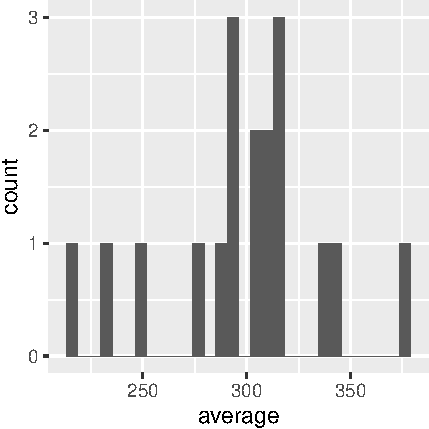
\includegraphics{visualization_files/figure-pdf/unnamed-chunk-2-1.pdf}

}

\end{figure}

Here, we work through a series of steps:

\begin{enumerate}
\def\labelenumi{\arabic{enumi}.}
\tightlist
\item
  \texttt{sleepstudy\ \%\textgreater{}\%} we first tell R we want to
  work with the dataset called \texttt{sleepstudy} and the
  \texttt{\%\textgreater{}\%} pipe symbol at the end of the line tells R
  that we want it to pass that dataset on to the next step for what
  happens next.
\item
  \texttt{group\_by(Subject)\ \%\textgreater{}\%} tells R that we want
  it to do something, here, group the rows of data according to the
  \texttt{Subject} (participant identity) coding variable, and pass the
  grouped data on to the next step for what happens following.
\item
  \texttt{summarise(average\ =\ mean(Reaction))\ \%\textgreater{}\%}
  tells R to take the grouped variable and calculate a summary, the mean
  Reaction score, for each group of observations for each participant.
  The \texttt{\%\textgreater{}\%} pipe at the end of the line tells R to
  pass the summary dataset of mean Reaction scores on to the next
  process.
\item
  \texttt{ggplot(aes(x\ =\ average))\ +} tells R that we want it to take
  these summary \texttt{average} Reaction scores and make a plot out of
  them.
\item
  \texttt{geom\_histogram()} tells R that we want a histogram plot.
\end{enumerate}

What you can see is that each line ending in a \texttt{\%\textgreater{}}
pipe passes something on to the next line. A following line takes the
output of the process coded in the preceding line, and works with it.

Each step is executed in turn, in strict sequence. This means that if I
delete line 3
\texttt{summarise(average\ =\ mean(Reaction))\ \%\textgreater{}\%} then
the following lines cannot work because the \texttt{ggplot()} function
will be looking for a variable \texttt{average} that does not yet exist.

\begin{tcolorbox}[enhanced jigsaw, opacitybacktitle=0.6, title=\textcolor{quarto-callout-warning-color}{\faExclamationTriangle}\hspace{0.5em}{Warning}, arc=.35mm, colbacktitle=quarto-callout-warning-color!10!white, colframe=quarto-callout-warning-color-frame, leftrule=.75mm, opacityback=0, breakable, titlerule=0mm, left=2mm, bottomrule=.15mm, toprule=.15mm, colback=white, coltitle=black, bottomtitle=1mm, toptitle=1mm, rightrule=.15mm]

\begin{itemize}
\tightlist
\item
  You can see that in the data processing part of the code, successive
  steps in data processing end in a pipe \texttt{\%\textgreater{}\%}.
\item
  In contrast, successive steps of the plotting code add \texttt{ggplot}
  elements line by line with each line (except the last) ending in a
  \texttt{+}.
\end{itemize}

\end{tcolorbox}

Notice that none of the processing steps actually changes the dataset
called \texttt{sleepstudy}. The results of the process exist and can be
used only within the sequence of steps that I have coded. If you want to
keep the results of processing steps, you need to assign an object name
to hold them, and I show how to do this, in the following.

You can read a clear explanation of pipes
\href{https://r4ds.had.co.nz/pipes.html}{here}.

\begin{tcolorbox}[enhanced jigsaw, opacitybacktitle=0.6, title=\textcolor{quarto-callout-tip-color}{\faLightbulb}\hspace{0.5em}{Tip}, arc=.35mm, colbacktitle=quarto-callout-tip-color!10!white, colframe=quarto-callout-tip-color-frame, leftrule=.75mm, opacityback=0, breakable, titlerule=0mm, left=2mm, bottomrule=.15mm, toprule=.15mm, colback=white, coltitle=black, bottomtitle=1mm, toptitle=1mm, rightrule=.15mm]

You can use the code you see:

\begin{itemize}
\tightlist
\item
  Each chunk of code is highlighted in the chapter.
\item
  If you hover a cursor over the highlighted code a little clipboard
  symbol appears in the top right of the code chunk.
\item
  Click on the clipboard symbol to copy the code, paste it into your own
  R-Studio instance.
\item
  Then \emph{experiment}: try out things like removing or commmenting
  out lines, or changing lines, to see what effect that has.
\item
  Breaking things, or changing things, helps to show what each bit of
  code does.
\end{itemize}

\end{tcolorbox}

\hypertarget{sec-ideas}{%
\section{Key ideas}\label{sec-ideas}}

Data visualization is not really about coding, as about thinking.

\begin{itemize}
\tightlist
\item
  What are our goals?
\item
  Why do we make some choices instead of others?
\end{itemize}

\hypertarget{sec-purposes}{%
\subsection{Purposes}\label{sec-purposes}}

A. Gelman \& Unwin (2013) outline the goals we may contemplate when we
produce or evaluate visual data displays. In general, they argue, we are
doing one or both of two things.

\begin{enumerate}
\def\labelenumi{\arabic{enumi}.}
\tightlist
\item
  Discovery
\item
  Communication
\end{enumerate}

In practice, this may involve the following (I paraphrase them, here).

\begin{enumerate}
\def\labelenumi{\arabic{enumi}.}
\tightlist
\item
  \textbf{Discovery goals}
\end{enumerate}

\begin{itemize}
\tightlist
\item
  Getting a sense of what is in a dataset, checking assumptions,
  confirming expectations, and looking for distinct patterns.
\item
  Making sense of the scale and complexity of the dataset.
\item
  Exploring the data to reveal unexpected aspects. As we will see, using
  small multiples (grids of plots) can often help with this.
\end{itemize}

\begin{enumerate}
\def\labelenumi{\arabic{enumi}.}
\setcounter{enumi}{1}
\tightlist
\item
  \textbf{Communication goals}
\end{enumerate}

\begin{itemize}
\tightlist
\item
  We communicate about our data to ourselves and to others. The process
  of constructing and evaluating a plot is often one way we speak to
  ourselves about own data, developing an understanding of what we have
  got. Once we have done this for ourselves, we can better figure out
  how to do it to benefit the understanding of an audience.
\item
  We often use a plot to tell a story: the story of our study, our data,
  or our insight and how we get to it.
\item
  We can use visualizations to attract attention and stimulate interest.
  Often, in presenting data to an audience through a talk or a report we
  need to use effective visualizations to ensure we get attention and
  that we locate the attention of our audience in the right places.
\end{itemize}

\hypertarget{sec-psychology-visualization}{%
\subsection{Psychological science of data
visualization}\label{sec-psychology-visualization}}

You will see a rich variety of data visualizations in media and in the
research literature. You will know that some choices, in the production
of those visualizations, appear to work better than others.

Some of the reasons why some choices work better will relate to what we
can understand in terms of the psychological science of how visual data
communication works. A useful recent review of relevant research is
presented by Franconeri et al. (2021).

Franconeri et al. (2021) provide a reason for working on visualizations:
they allow us humans to process an array of information at once, often
faster than if we were reading about the information, bit by bit.
Effective visualization, then, is about harnessing the power of the
human visual system, or visual cognition, for quick, efficient,
information processing. Critically for science, in addition,
visualizations can be more effective for discovering or communicating
the critical features of data than summary statistics, as we shall see.

In producing visualizations, we often work with a vocabulary or palette
of objects or visual elements. Franconeri et al. (2021) discuss how
visualizations rely on visual channels to transform numbers into images
that we can process visually.

\begin{itemize}
\tightlist
\item
  Dot plots and scatterplots represent values as position.
\item
  Bar graphs represent values as position (the heights of the tops of
  bars) but also as lengths.
\item
  Angles are presented when we connect points to form a line, allowing
  us to encode the differences between points.
\item
  Intensity can be presented through variation in luminance contrast or
  colour saturation.
\end{itemize}

These channels can be ordered by how precisely they have been found to
communicate different numeric values to the viewer. Your audience may
more accurately perceive the difference between two quantities if you
communicate that difference through the difference in the location of
two points than if you ask your audience to compare the angles of two
lines or the intensity of two colour spots.

In constructing data visualizations, we often work with conventions,
established through common practice in a research tradition. For
example, if you are producing a scatterplot, then most of the time your
audience will expect to see the outcome (or dependent variable)
represented by the vertical height (on the y-axis) of points. And your
audience will expect that higher points represent larger quantities of
the y-axis variable.

In constructing visualizations, we need to be aware of the cognitive
work that we require the audience to do. Comparisons are harder,
requiring more processing and imposing more load on working memory. You
can help your reader by guiding their attention, by grouping or ordering
visual elements to identify the most important comparisons. We can vary
colour and shape to group or distinguish visual elements. We can add
annotation or elements like lines or arrows to guide attention.

Visualizations are presented in context, whether in presentations or in
reports. This context should be provided, by you the producer, with the
intention to support the communication of your key messages. A visual
representation, a plot, will be presented with a title, maybe a title
note, maybe with annotation in the plot, and maybe with accompanying
text. You should use these textual elements to lead your audience, to
help them make sense of what they are looking at.

The diversity of audiences means that we should habitually add alt text
for data visualizations to help those who use screen readers by
providing a summary description of what images show. This chapter has
been written using \texttt{Quarto} and rendered to .html with alt text
included along with all images. Please do let me know if you are using a
screen reader and the alt text description is or is not so helpful.

You can read a helpful explanation of alt text
\href{https://medium.com/nightingale/writing-alt-text-for-data-visualization-2a218ef43f81}{here}.

If you use colour in images then we should use colour bind colour
palettes.

You can read about using colour blind palettes
\href{http://www.cookbook-r.com/Graphs/Colors_(ggplot2)/}{here} or
\href{https://cran.r-project.org/web/packages/viridis/vignettes/intro-to-viridis.html}{here}.

In the following practical exercises, we work with many of the insights
in our construction of visualizations.

\hypertarget{sec-quick-start}{%
\section{A quick start}\label{sec-quick-start}}

We can get started before we understand in depth the key ideas or the
coding steps. This will help to show where we are going. We will work
with the \texttt{sleepstudy} dataset.

I will model the process, to give you an example workflow:

\begin{itemize}
\tightlist
\item
  the data, where they come from --- what we can find out;
\item
  how we approach the data --- what we \emph{expect} to see;
\item
  how we visualize the data --- discovery, communication.
\end{itemize}

\hypertarget{sec-sleep-study-data}{%
\subsection{Sleepstudy data}\label{sec-sleep-study-data}}

When we work with R, we usually work with functions like
\texttt{ggplot()} provided in libraries like \texttt{ggplot2} (Wickham,
2016). These libraries typically provide not only functions but also
datasets that we can use for demonstration and learning.

The \texttt{lme4} library (Bates et al., 2015) provides the
\texttt{sleepstudy} dataset and we will take a look at these data to
offer a taste of what we can learn to do. Usually, information about the
R libraries we use will be located on the
\href{https://cran.r-project.org}{Comprehensive R Archive Network
(CRAN)} web pages, and we can find the technical reference information
for \href{https://cran.r-project.org/web/packages/lme4/lme4.pdf}{lme4}
in the CRAN reference manual for the library, where we see that the
\texttt{sleepstudy} data are from a study reported by (Belenky et al.,
2003). The manual says that the \texttt{sleepstudy} dataset comprises:

\begin{quote}
A data frame with 180 observations on the following 3 variables.
{[}1.{]} Reaction -- Average reaction time (ms) {[}2.{]} Days -- Number
of days of sleep deprivation {[}3.{]} Subject -- Subject number on which
the observation was made.
\end{quote}

We can take a look at the first few rows of the dataset.

\begin{Shaded}
\begin{Highlighting}[]
\NormalTok{sleepstudy }\SpecialCharTok{\%\textgreater{}\%}
    \FunctionTok{head}\NormalTok{(}\AttributeTok{n =} \DecValTok{4}\NormalTok{)}
\end{Highlighting}
\end{Shaded}

\begin{verbatim}
  Reaction Days Subject
1 249.5600    0     308
2 258.7047    1     308
3 250.8006    2     308
4 321.4398    3     308
\end{verbatim}

What we are looking at are:

\begin{quote}
The average reaction time per day (in milliseconds) for subjects in a
sleep deprivation study. Days 0-1 were adaptation and training (T1/T2),
day 2 was baseline (B); sleep deprivation started after day 2.
\end{quote}

The abstract for Belenky et al. (2003) tells us that participants were
deprived of sleep and the impact of relative deprivation was tested
using a cognitive vigilance task for which the reaction times of
responses were recorded.

So, we can \emph{expect to find}:

\begin{itemize}
\tightlist
\item
  A set of rows corresponding to multiple observations for each
  participant (\texttt{Subject})
\item
  A reaction time value for each participant (\texttt{Reaction})
\item
  Recorded on each \texttt{Day}
\end{itemize}

\hypertarget{sec-sleepstudy-histogram}{%
\subsection{Discovery and
communication}\label{sec-sleepstudy-histogram}}

In data analysis work, we often begin with the objective to understand
the structure or the nature of the data we are working with.

You can call this the \emph{discovery} phase:

\begin{itemize}
\tightlist
\item
  what have we got?
\item
  does it match our expectations?
\end{itemize}

If these are reaction time data (collected in an cognitive experiment)
do they look like cognitive reaction time data \emph{should} look? We
would expect to see a skewed distribution of observed reaction times
distributed around an average located somewhere in the range 200-700ms.

Figure~\ref{fig-sleep-study-histogram} represents the distribution of
reaction times in the \texttt{sleepstudy} dataset.

I provide notes on the code steps that result in the plot. Click on the
\texttt{Notes} tab to see them. Later, I will discuss some of these
elements.

\section{Plot}

\begin{Shaded}
\begin{Highlighting}[]
\NormalTok{sleepstudy }\SpecialCharTok{\%\textgreater{}\%}
  \FunctionTok{ggplot}\NormalTok{(}\FunctionTok{aes}\NormalTok{(}\AttributeTok{x =}\NormalTok{ Reaction)) }\SpecialCharTok{+}
  \FunctionTok{geom\_histogram}\NormalTok{(}\AttributeTok{binwidth =} \DecValTok{15}\NormalTok{) }\SpecialCharTok{+}
  \FunctionTok{geom\_vline}\NormalTok{(}\AttributeTok{xintercept =} \FunctionTok{mean}\NormalTok{(sleepstudy}\SpecialCharTok{$}\NormalTok{Reaction), }
             \AttributeTok{colour =} \StringTok{"red"}\NormalTok{, }\AttributeTok{linetype =} \StringTok{\textquotesingle{}dashed\textquotesingle{}}\NormalTok{, }\AttributeTok{size =} \FloatTok{1.5}\NormalTok{) }\SpecialCharTok{+}
  \FunctionTok{annotate}\NormalTok{(}\StringTok{"text"}\NormalTok{, }\AttributeTok{x =} \DecValTok{370}\NormalTok{, }\AttributeTok{y =}\DecValTok{20}\NormalTok{, }
                    \AttributeTok{colour =} \StringTok{"red"}\NormalTok{, }
                    \AttributeTok{label =} \StringTok{"Average value shown in red"}\NormalTok{) }\SpecialCharTok{+}
  \FunctionTok{theme\_bw}\NormalTok{()}
\end{Highlighting}
\end{Shaded}

\begin{verbatim}
Warning: Using `size` aesthetic for lines was deprecated in ggplot2 3.4.0.
i Please use `linewidth` instead.
\end{verbatim}

\begin{figure}[H]

{\centering 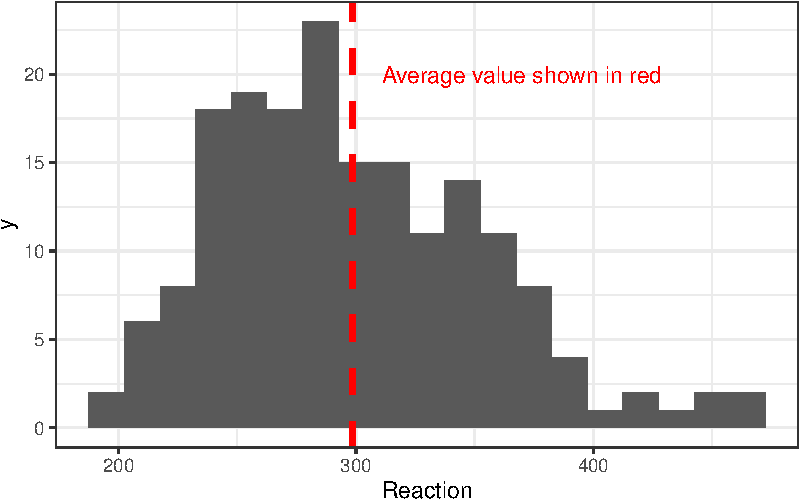
\includegraphics{visualization_files/figure-pdf/fig-sleep-study-histogram-1.pdf}

}

\caption{\label{fig-sleep-study-histogram}Figure showing a histogram of
\texttt{sleepstudy} reaction time data}

\end{figure}

\section{Notes}

The plotting code pipes the data into the plotting code steps to produce
the plot. You can see some elements that will be familiar to you and
some new elements.

\begin{Shaded}
\begin{Highlighting}[]
\NormalTok{sleepstudy }\SpecialCharTok{\%\textgreater{}\%}
  \FunctionTok{ggplot}\NormalTok{(}\FunctionTok{aes}\NormalTok{(}\AttributeTok{x =}\NormalTok{ Reaction)) }\SpecialCharTok{+}
  \FunctionTok{geom\_histogram}\NormalTok{(}\AttributeTok{binwidth =} \DecValTok{15}\NormalTok{) }\SpecialCharTok{+}
  \FunctionTok{geom\_vline}\NormalTok{(}\AttributeTok{xintercept =} \FunctionTok{mean}\NormalTok{(sleepstudy}\SpecialCharTok{$}\NormalTok{Reaction), }
             \AttributeTok{colour =} \StringTok{"red"}\NormalTok{, }\AttributeTok{linetype =} \StringTok{\textquotesingle{}dashed\textquotesingle{}}\NormalTok{, }\AttributeTok{size =} \FloatTok{1.5}\NormalTok{) }\SpecialCharTok{+}
  \FunctionTok{annotate}\NormalTok{(}\StringTok{"text"}\NormalTok{, }\AttributeTok{x =} \DecValTok{370}\NormalTok{, }\AttributeTok{y =}\DecValTok{20}\NormalTok{, }
                    \AttributeTok{colour =} \StringTok{"red"}\NormalTok{, }
                    \AttributeTok{label =} \StringTok{"Average value shown in red"}\NormalTok{) }\SpecialCharTok{+}
  \FunctionTok{theme\_bw}\NormalTok{()}
\end{Highlighting}
\end{Shaded}

Let's go through the code step-by-step:

\begin{enumerate}
\def\labelenumi{\arabic{enumi}.}
\tightlist
\item
  \texttt{sleepstudy\ \%\textgreater{}\%} asks R to take the
  \texttt{sleepstudy} dataset and \texttt{\%\textgreater{}\%} pipe it to
  the next steps for processing.
\item
  \texttt{ggplot(aes(x\ =\ Reaction))\ +} takes the \texttt{sleepstudy}
  data and asks R to use the \texttt{ggplot()} function to produce a
  plot.
\item
  \texttt{aes(x\ =\ Reaction)} tells R that in the plot we want it to
  map the \texttt{Reaction} variable values to locations on the x-axis:
  this is the aesthetic mapping.
\item
  \texttt{geom\_histogram(binwidth\ =\ 15)\ +} tells R to produce a
  histogram then add a step.
\item
  \texttt{geom\_vline(...)\ +} tells R we want to draw vertical line.
\item
  \texttt{xintercept\ =\ mean(sleepstudy\$Reaction),\ ...} tells R to
  draw the vertical line at the mean value of the variable
  \texttt{Reaction} in the \texttt{sleepstudy} dataset.
\item
  \texttt{colour\ =\ "red",\ linetype\ =\ \textquotesingle{}dashed\textquotesingle{},\ size\ =\ 1.5}
  tells R we want the vertical line to be red, dashed and 1.5 times the
  usual size.
\item
  \texttt{annotate("text",\ ...)} tells R we want to add a text note.
\item
  \texttt{x\ =\ 370,\ y\ =20,\ ...} tells R we want the note added at
  the x,y coordinates given.
\item
  \texttt{colour\ =\ "red",\ ..;} and we want the text in red.
\item
  \texttt{...label\ =\ "Average\ value\ shown\ in\ red")\ +} tells R we
  want the text note to say that this is where the average is.
\item
  \texttt{theme\_bw()} lastly, we change the theme.
\end{enumerate}

Figure~\ref{fig-sleep-study-histogram} shows a distribution of reaction
times, ranging from about 200ms to 500ms. The distribution has a peak
around 300ms. The location of the mean is shown with a dashed red line.
The distribution includes a long tail of longer times. This \emph{is}
pretty much what we would expect to see.

We may wish to communicate the information we gain through using this
histogram, in a presentation or in a report.

\hypertarget{sec-sleepstudy-scatter}{%
\subsection{Discovery and communication}\label{sec-sleepstudy-scatter}}

Let us imagine that it is our study. (Here, we shall not concern
ourselves too much --- with apologies --- with understanding what the
original study authors actually did.)

If we are looking at the impact of sleep deprivation on cognitive
performance, we might predict that reaction times got longer (responses
slowed) as the study progressed. Is that what we see?

To examine the association between two variables, we often use
scatterplots. Figure~\ref{fig-sleep-study-scatterplot-all} is a
scatterplot indicating the possible association between reaction time
and days in the \texttt{sleepstudy} data. Points are ordered on x-axis
from 0 to 9 days, on y-axis from 200 to 500 ms reaction time.

I provide notes on the code steps that result in the plot. Click on the
\texttt{Notes} tab to see them. Later, I will discuss some of these
elements.

\section{Plot}

\begin{Shaded}
\begin{Highlighting}[]
\NormalTok{sleepstudy }\SpecialCharTok{\%\textgreater{}\%}
  \FunctionTok{ggplot}\NormalTok{(}\FunctionTok{aes}\NormalTok{(}\AttributeTok{x =}\NormalTok{ Days, }\AttributeTok{y =}\NormalTok{ Reaction)) }\SpecialCharTok{+}
  \FunctionTok{geom\_point}\NormalTok{(}\AttributeTok{size =} \FloatTok{1.5}\NormalTok{, }\AttributeTok{alpha =}\NormalTok{ .}\DecValTok{5}\NormalTok{) }\SpecialCharTok{+} 
  \FunctionTok{scale\_x\_continuous}\NormalTok{(}\AttributeTok{breaks =} \FunctionTok{c}\NormalTok{(}\DecValTok{0}\NormalTok{, }\DecValTok{3}\NormalTok{, }\DecValTok{6}\NormalTok{, }\DecValTok{9}\NormalTok{)) }\SpecialCharTok{+}
  \FunctionTok{theme\_bw}\NormalTok{()}
\end{Highlighting}
\end{Shaded}

\begin{figure}[H]

{\centering 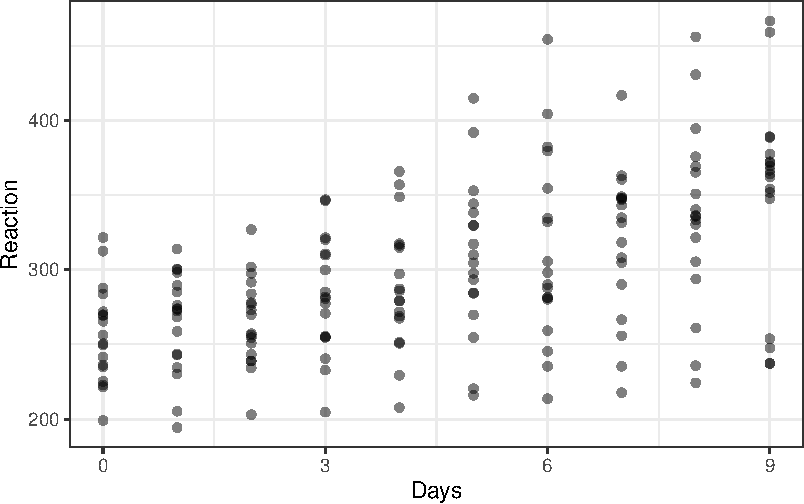
\includegraphics{visualization_files/figure-pdf/fig-sleep-study-scatterplot-all-1.pdf}

}

\caption{\label{fig-sleep-study-scatterplot-all}Figure showing a
scatterplot of the relation between reaction time and days in the
\texttt{sleepstudy} data}

\end{figure}

\section{Notes}

Notice the numbered steps in producing this plot.

\begin{Shaded}
\begin{Highlighting}[numbers=left,,]
\NormalTok{sleepstudy }\SpecialCharTok{\%\textgreater{}\%} 
  \FunctionTok{ggplot}\NormalTok{(}\FunctionTok{aes}\NormalTok{(}\AttributeTok{x =}\NormalTok{ Days, }\AttributeTok{y =}\NormalTok{ Reaction)) }\SpecialCharTok{+}
  \FunctionTok{geom\_point}\NormalTok{() }\SpecialCharTok{+} 
  \FunctionTok{scale\_x\_continuous}\NormalTok{(}\AttributeTok{breaks =} \FunctionTok{c}\NormalTok{(}\DecValTok{0}\NormalTok{, }\DecValTok{3}\NormalTok{, }\DecValTok{6}\NormalTok{, }\DecValTok{9}\NormalTok{)) }\SpecialCharTok{+}
  \FunctionTok{theme\_bw}\NormalTok{()}
\end{Highlighting}
\end{Shaded}

\begin{enumerate}
\def\labelenumi{\arabic{enumi}.}
\tightlist
\item
  Name the dataset: the dataset is called \texttt{sleepstudy} in the
  \texttt{lme4} library which makes it available therefore we use this
  name to specify it.
\item
  \texttt{sleepstudy\ \%\textgreater{}\%} uses the
  \texttt{\%\textgreater{}\%} pipe operator to pass this dataset to
  \texttt{ggplot()} to work with, in creating the plot. Because
  \texttt{ggplot()} now knows about the \texttt{sleepstudy} data, we can
  next specify what aesthetic mappings we need to use.
\item
  \texttt{ggplot(aes(x\ =\ Days,\ y\ =\ Reaction))\ +} tells R that we
  want to map \texttt{Days} information to x-axis position and
  \texttt{Reaction} (response time) information to y-axis position.
\item
  \texttt{geom\_point()\ +} tells R that we want to locate points --
  creating a scatterplot -- at the paired x-axis and y-xis coordinates.
\item
  \texttt{scale\_x\_continuous(breaks\ =\ c(0,\ 3,\ 6,\ 9))\ +} is new:
  we tell R that we want the x-axis tick labels -- the numbers R shows
  as labels on the x-axis -- at the values 0, 3, 6, 9 only.
\item
  \texttt{theme\_bw()} requires R to make the plot background white and
  the foreground plot elements black.
\end{enumerate}

You can find more information on \texttt{scale\_} functions in the
\texttt{ggplot2} reference information.

\url{https://ggplot2.tidyverse.org/reference/scale_continuous.html}

The plot suggests that reaction time increases with increasing number of
days.

In producing this plot, we are both (1.) engaged in discovery and,
potentially, (2.) able to do communication.

\begin{enumerate}
\def\labelenumi{\arabic{enumi}.}
\tightlist
\item
  Discovery: is the relation between variables what we should expect,
  given our assumptions?
\item
  Communication: to ourselves and others, what relation do we observe,
  given our sample?
\end{enumerate}

At this time, we have used and discussed scatterplots before, why we use
them, how we write code to produce them, and how we read them.

With two additional steps we can significantly increase the power of the
visualization. Figure~\ref{fig-sleep-study-scatterplot-by-subject} is a
grid of scatterplots indicating the possible association between
reaction time and days separately for each participant.

Again, I hide an explanation of the coding steps in the \texttt{Notes}
tab: the interested reader can click on the tab to view the step-by-step
guide to what is happening.

\section{Plot}

\begin{Shaded}
\begin{Highlighting}[]
\NormalTok{sleepstudy }\SpecialCharTok{\%\textgreater{}\%}
  \FunctionTok{group\_by}\NormalTok{(Subject) }\SpecialCharTok{\%\textgreater{}\%}
  \FunctionTok{mutate}\NormalTok{(}\AttributeTok{average =} \FunctionTok{mean}\NormalTok{(Reaction)) }\SpecialCharTok{\%\textgreater{}\%}
  \FunctionTok{ungroup}\NormalTok{() }\SpecialCharTok{\%\textgreater{}\%}
  \FunctionTok{mutate}\NormalTok{(}\AttributeTok{Subject =} \FunctionTok{fct\_reorder}\NormalTok{(Subject, average)) }\SpecialCharTok{\%\textgreater{}\%}
  \FunctionTok{ggplot}\NormalTok{(}\FunctionTok{aes}\NormalTok{(}\AttributeTok{x =}\NormalTok{ Days, }\AttributeTok{y =}\NormalTok{ Reaction)) }\SpecialCharTok{+}
  \FunctionTok{geom\_point}\NormalTok{() }\SpecialCharTok{+} 
  \FunctionTok{geom\_line}\NormalTok{() }\SpecialCharTok{+}
  \FunctionTok{scale\_x\_continuous}\NormalTok{(}\AttributeTok{breaks =} \FunctionTok{c}\NormalTok{(}\DecValTok{0}\NormalTok{, }\DecValTok{3}\NormalTok{, }\DecValTok{6}\NormalTok{, }\DecValTok{9}\NormalTok{)) }\SpecialCharTok{+}
  \FunctionTok{facet\_wrap}\NormalTok{(}\SpecialCharTok{\textasciitilde{}}\NormalTok{ Subject) }\SpecialCharTok{+}
  \FunctionTok{theme\_bw}\NormalTok{()}
\end{Highlighting}
\end{Shaded}

\begin{figure}[H]

{\centering 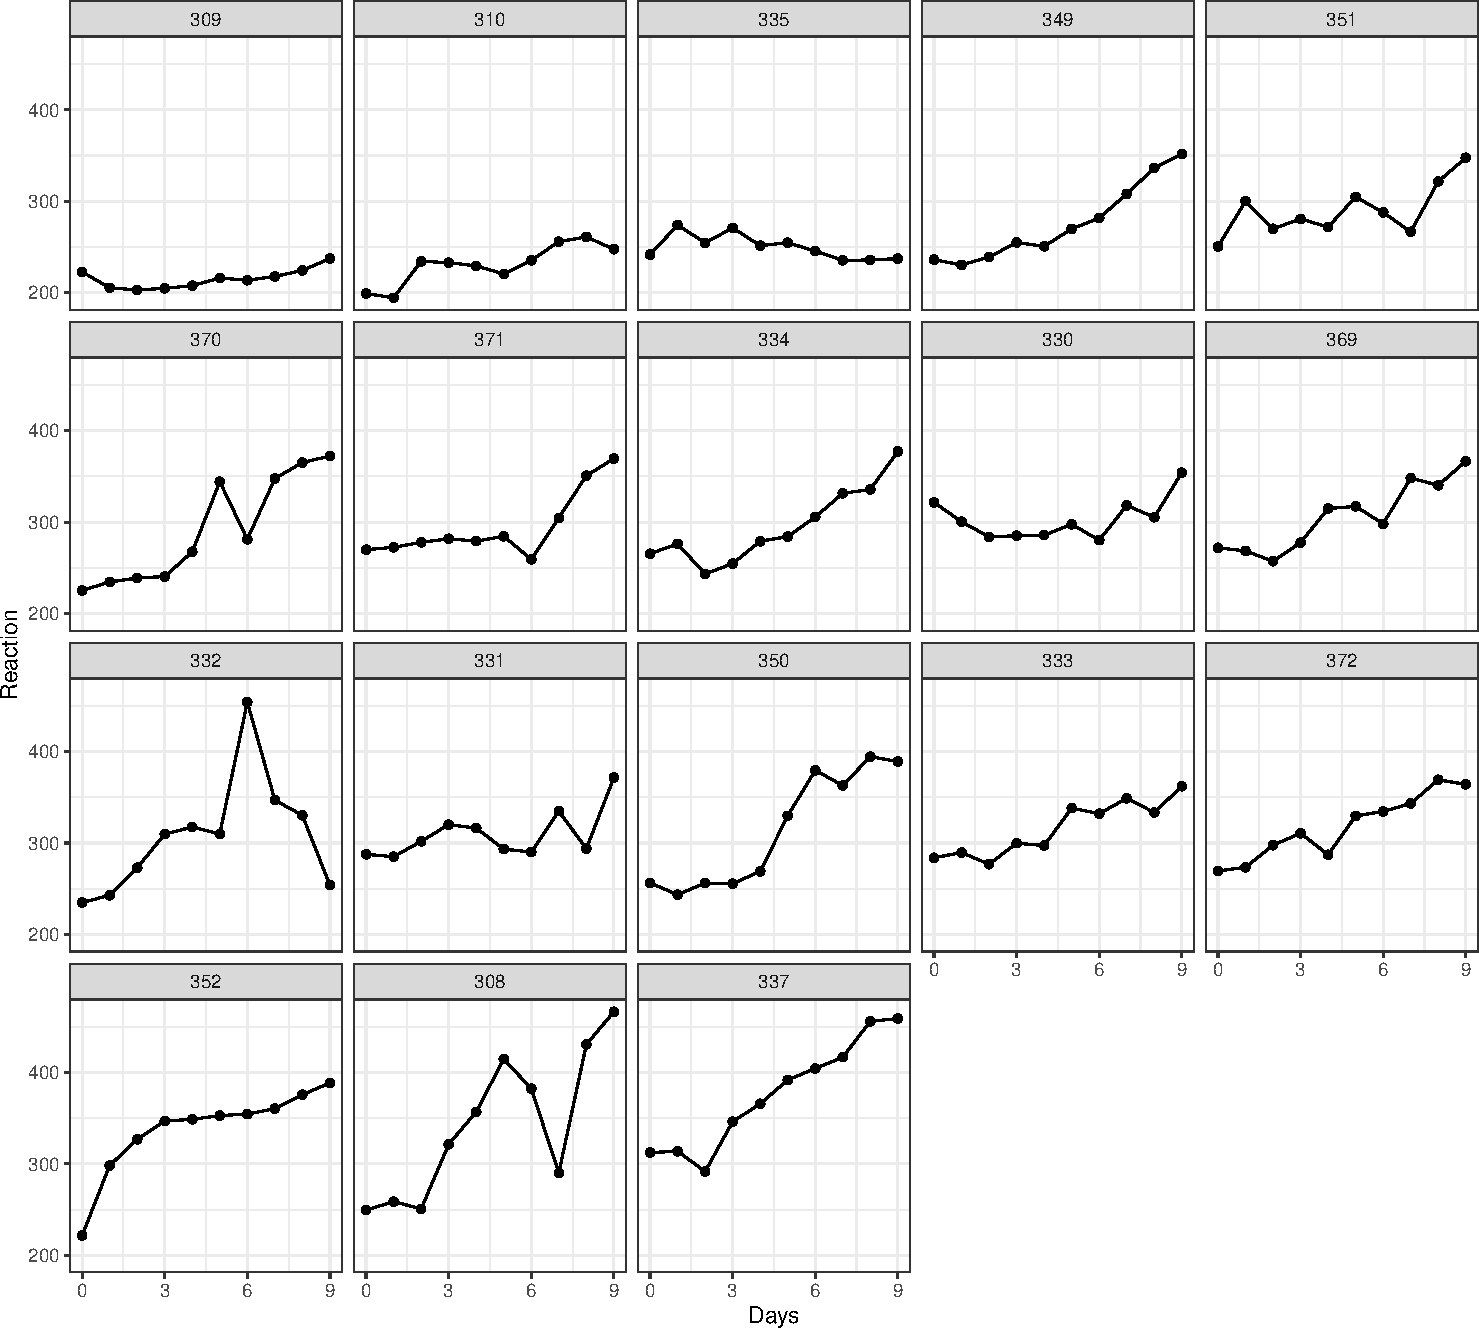
\includegraphics{visualization_files/figure-pdf/fig-sleep-study-scatterplot-by-subject-1.pdf}

}

\caption{\label{fig-sleep-study-scatterplot-by-subject}Figure showing a
scatterplot of the relation between reaction time and days: here, we
plot the data for each participant separately}

\end{figure}

\section{Notes}

Notice the numbered steps in producing this plot.

\begin{Shaded}
\begin{Highlighting}[numbers=left,,]
\NormalTok{sleepstudy }\SpecialCharTok{\%\textgreater{}\%}
  \FunctionTok{group\_by}\NormalTok{(Subject) }\SpecialCharTok{\%\textgreater{}\%}
  \FunctionTok{mutate}\NormalTok{(}\AttributeTok{average =} \FunctionTok{mean}\NormalTok{(Reaction)) }\SpecialCharTok{\%\textgreater{}\%}
  \FunctionTok{ungroup}\NormalTok{() }\SpecialCharTok{\%\textgreater{}\%}
  \FunctionTok{mutate}\NormalTok{(}\AttributeTok{Subject =} \FunctionTok{fct\_reorder}\NormalTok{(Subject, average)) }\SpecialCharTok{\%\textgreater{}\%}
  \FunctionTok{ggplot}\NormalTok{(}\FunctionTok{aes}\NormalTok{(}\AttributeTok{x =}\NormalTok{ Days, }\AttributeTok{y =}\NormalTok{ Reaction)) }\SpecialCharTok{+}
  \FunctionTok{geom\_point}\NormalTok{() }\SpecialCharTok{+} 
  \FunctionTok{geom\_line}\NormalTok{() }\SpecialCharTok{+}
  \FunctionTok{scale\_x\_continuous}\NormalTok{(}\AttributeTok{breaks =} \FunctionTok{c}\NormalTok{(}\DecValTok{0}\NormalTok{, }\DecValTok{3}\NormalTok{, }\DecValTok{6}\NormalTok{, }\DecValTok{9}\NormalTok{)) }\SpecialCharTok{+}
  \FunctionTok{facet\_wrap}\NormalTok{(}\SpecialCharTok{\textasciitilde{}}\NormalTok{ Subject) }\SpecialCharTok{+}
  \FunctionTok{theme\_bw}\NormalTok{()}
\end{Highlighting}
\end{Shaded}

You can see that the block of code combines \emph{data processing} and
\emph{data plotting} steps. Let's look at the data processing steps then
the plotting steps in order.

First: why are we doing this? My aim is to produce a plot in which I
show the association between \texttt{Days} and \texttt{Reaction} for
each \texttt{Subject} individually. I suspect that the association
between \texttt{Days} and \texttt{Reaction} may be stronger -- so the
trend will be steeper -- for participants who are slower overall. I
suspect this because, given experience, I know that slower, less
accurate, participants tend to show larger effects.

So: in order to get a grid of plots, one plot for each \texttt{Subject},
in order of the average \texttt{Reaction} for each individual
\texttt{Subject}, I need to first calculate the average
\texttt{Reaction} then order the dataset rows by those averages. I do
that in steps, using pipes to feed information from one step to the next
step, as follows.

\begin{enumerate}
\def\labelenumi{\arabic{enumi}.}
\tightlist
\item
  \texttt{sleepstudy\ \%\textgreater{}\%} tells R what data I want to
  use, and pipe it to the next step.
\item
  \texttt{group\_by(Subject)} tells R I want it to work with data (rows)
  grouped by \texttt{Subject} identity code, \texttt{\%\textgreater{}\%}
  piping the grouped form of the data forward to the next step
\item
  \texttt{mutate(average\ =\ mean(Reaction))} uses \texttt{mutate()} to
  create a new variable \texttt{average} which I calculate as the
  \texttt{mean()} of \texttt{Reaction}, piping the data with this
  additional variable \texttt{\%\textgreater{}\%} forward to the next
  step.
\item
  \texttt{ungroup()\ \%\textgreater{}\%} tells R I want it to go back to
  working with the data in rows not grouped rows, and pipe the now
  ungrouped form of the data to the next step.
\item
  \texttt{mutate(Subject\ =\ fct\_reorder(Subject,\ average))} tells R I
  want it to sort the rows of the whole \texttt{sleepstudy} dataset in
  order, moving groups of rows identified by \texttt{Subject} so that
  data for \texttt{Subject} codes associated with faster times are
  located near the top of the dataset.
\end{enumerate}

These data, ordered by \texttt{Subject} by the average \texttt{Reaction}
for each participant, are then \texttt{\%\textgreater{}\%} piped to
\texttt{ggplot} to create a plot.

\begin{enumerate}
\def\labelenumi{\arabic{enumi}.}
\setcounter{enumi}{5}
\tightlist
\item
  \texttt{ggplot(aes(x\ =\ Days,\ y\ =\ Reaction))\ +} specifies the
  aesthetic mappings, as before.
\item
  \texttt{geom\_point()\ +} asks R to locate points at the x-axis,
  y-axis coordinates, creating a scatterplot, as before.
\item
  \texttt{geom\_line()\ +} is new: I want R to connect the points,
  showing the trend in the association between \texttt{Days} and
  \texttt{Reaction} for each person.
\item
  \texttt{scale\_x\_continuous(breaks\ =\ c(0,\ 3,\ 6,\ 9))\ +} fixes
  the x-axis labels, as before.
\item
  \texttt{facet\_wrap(\textasciitilde{}\ Subject)\ +} is the big new
  step: I ask R to plot a separate scatterplot for the data for each
  individual \texttt{Subject}.
\end{enumerate}

You can see more information about facetting here:

\url{https://ggplot2.tidyverse.org/reference/facet_wrap.html}

In short, with the \texttt{facet\_wrap(\textasciitilde{}\ .)} function,
we are asking R to subset the data by a grouping variable, specified
\texttt{(\textasciitilde{}\ .)} by replacing the dot with the name of
the variable.

Notice that I use \texttt{\%\textgreater{}\%} pipes to move the data
processing forward, step by step. But I use \texttt{+} to add plot
elements, layer by layer.

Figure Figure~\ref{fig-sleep-study-scatterplot-by-subject} is a grid or
lattice of scatterplots \emph{revealing} how the possible association
between reaction time and days varies quite substantially between the
participants in the \texttt{sleepstudy} data. Most plots indicate that
reaction time increases with increasing number of days. However,
different participants show this trend to differing extents.

What are the two additions I made to the conventional scatterplot code?

\begin{itemize}
\tightlist
\item
  I calculated the average reaction time per participant, and I ordered
  the data by those averages.
\item
  I \emph{facetted} the plots, breaking them out into separate
  scatterplots per participant.
\end{itemize}

Why would you do this? Variation between people or groups, in effects or
in average outcomes, are often to be found in psychological data
(Vasishth \& Gelman, 2021). The variation between people that we see in
these data --- in the average response reaction time, and in how days
affects times --- would motivate the use of linear mixed-effects models
to analyze the way that sleep patterns affect responses in the sleep
study (Pinheiro \& Bates, 2000).

\begin{tcolorbox}[enhanced jigsaw, opacitybacktitle=0.6, title=\textcolor{quarto-callout-tip-color}{\faLightbulb}\hspace{0.5em}{Tip}, arc=.35mm, colbacktitle=quarto-callout-tip-color!10!white, colframe=quarto-callout-tip-color-frame, leftrule=.75mm, opacityback=0, breakable, titlerule=0mm, left=2mm, bottomrule=.15mm, toprule=.15mm, colback=white, coltitle=black, bottomtitle=1mm, toptitle=1mm, rightrule=.15mm]

The data processing and plotting functions in the \texttt{tidyverse}
collection of libraries enable us to discover and to communicate
variation in behaviours that should strengthen our and others'
scientific understanding.

\end{tcolorbox}

\hypertarget{summary-quick-start-lessons}{%
\subsection{Summary: Quick start
lessons}\label{summary-quick-start-lessons}}

What we have seen, so far, is that we can make dramatic changes to the
appearance of visualizations (e.g., through faceting) and also that we
can exert fine control over the details (e.g., adjusting scale labels).
What we need to stop and consider are what we want to do (and why), in
what order.

We have seen how we can feed a data process into a plot to first prepare
then produce the plot in a sequence of steps. In processing the data, we
can take some original data and extract or calculate information that we
can use for our plotting e.g.~calculating the mean of a distribution in
order to then highlight where that mean is located.

We have also seen the use of plots, and the editing of their appearance,
to represent information visually. We can verbalize the thought process
behind the production of these plots through a series of questions.

\begin{enumerate}
\def\labelenumi{\arabic{enumi}.}
\tightlist
\item
  Are we looking at the distribution of one variable (if yes: consider a
  histogram) or are we comparing the distributions of two or more
  variables (if yes: consider a scatterplot)?
\item
  Is there a salient feature of the plot we want to draw the attention
  of the audience to? We can add a visual element (like a line) and
  annotation text to guide the audience.
\item
  Are we interested in variation between sub-sets of the data? We can
  facet the plot to examine variation between sub-sets (facets) enabling
  the comparison of trends.
\end{enumerate}

\hypertarget{sec-practical-visualization}{%
\section{A practical guide to visualization
ideas}\label{sec-practical-visualization}}

In this guide, we illustrate some of the ideas about visualization we
discussed at the start, working with practical coding examples. We will
be working with real data from a published research project. We are
going to focus the practical coding examples on the data collected for
the analysis reported by Ricketts et al. (2021).

We will focus on working with the data from one of the tasks, in one of
the studies reported by Ricketts et al. (2021).

\begin{itemize}
\tightlist
\item
  This means that you can consolidate your learning by applying the same
  code moves to data from the other task in the same study, or to data
  from the other study.
\item
  In applying code to other data, you will need to be aware of
  differences in, say, the way that some things like the outcome
  response variable are coded.
\end{itemize}

You can then further extend your development by trying out the coding
moves for yourself using the data collected by Rodríguez-Ferreiro et al.
(2020).

\begin{itemize}
\tightlist
\item
  These data are from a quite distinct kind of investigation, on a
  different research topic than the topic we will be exploring through
  our working examples.
\item
  However, some aspects of the data structure are similar.
\item
  Critically, the data are provided with comprehensive documentation.
\end{itemize}

\hypertarget{sec-set-up}{%
\subsection{Set up for coding}\label{sec-set-up}}

To do our practical work, we will need functions and data. We get these
at the start of our workflow.

\hypertarget{sec-libraries}{%
\subsubsection{Get libraries}\label{sec-libraries}}

We are going to need the \texttt{lme4,\ patchwork,\ psych} and
\texttt{tidyverse} libraries of functions and data.

\begin{Shaded}
\begin{Highlighting}[]
\FunctionTok{library}\NormalTok{(ggeffects)}
\FunctionTok{library}\NormalTok{(patchwork)}
\FunctionTok{library}\NormalTok{(psych)}
\FunctionTok{library}\NormalTok{(tidyverse)}
\end{Highlighting}
\end{Shaded}

\hypertarget{sec-get-data}{%
\subsubsection{Get the data}\label{sec-get-data}}

You can access the data we are going to use in two different ways.

\hypertarget{sec-from-repros}{%
\paragraph{Get the data from project
repositories}\label{sec-from-repros}}

The data associated with both (Ricketts et al., 2021) and
(Rodríguez-Ferreiro et al., 2020) are freely available through project
repositories on the Open Science Framework web pages.

You can get the data from the Ricketts et al. (2021)
\href{https://www.sciencedirect.com/science/article/pii/S095947522100027X}{paper}
through the repository located
\href{https://osf.io/e5gzk/?view_only=038118528c7c426c9729983f54138c88}{here}.

You can get the data from the Rodríguez-Ferreiro et al. (2020)
\href{https://peerj.com/articles/9511/}{paper} through the repository
located \href{https://osf.io/j29fn/}{here}.

These data are associated with full explanations of data collection
methods, materials, data processing and data analysis code. You can
review the papers and the repository material guides for further
information.

In the following, I am going to abstract summary information about the
Ricketts et al. (2021) study and data. I shall leave you to do the same
for the Rodríguez-Ferreiro et al. (2020) study.

\hypertarget{sec-download}{%
\paragraph{Get the data through a downloadable
archive}\label{sec-download}}

Download the \href{files/data.zip}{data.zip} files folder and upload the
files to RStudio Server.

The folder includes the Ricketts et al. (2021) data files:

\begin{itemize}
\item
  \texttt{concurrent.orth\_2020-08-11.csv}
\item
  \texttt{concurrent.sem\_2020-08-11.csv}
\item
  \texttt{long.orth\_2020-08-11.csv}
\item
  \texttt{long.sem\_2020-08-11.csv}
\end{itemize}

The folder also includes the Rodríguez-Ferreiro et al. (2020) data
files:

\begin{itemize}
\tightlist
\item
  \texttt{PrimDir-111019\_English.csv}
\item
  \texttt{PrimInd-111019\_English.csv}
\end{itemize}

\begin{tcolorbox}[enhanced jigsaw, opacitybacktitle=0.6, title=\textcolor{quarto-callout-warning-color}{\faExclamationTriangle}\hspace{0.5em}{Warning}, arc=.35mm, colbacktitle=quarto-callout-warning-color!10!white, colframe=quarto-callout-warning-color-frame, leftrule=.75mm, opacityback=0, breakable, titlerule=0mm, left=2mm, bottomrule=.15mm, toprule=.15mm, colback=white, coltitle=black, bottomtitle=1mm, toptitle=1mm, rightrule=.15mm]

\begin{itemize}
\tightlist
\item
  These data files are collected together in a folder for download, for
  your convenience, but the \emph{version of record} for the data for
  each study comprise the files located on the OSF repositories
  associated with the original articles.
\end{itemize}

\end{tcolorbox}

\hypertarget{sec-ricketts-study}{%
\subsection{Information about the Ricketts study and the
datasets}\label{sec-ricketts-study}}

Ricketts et al. (2021) conducted an investigation of word learning in
school-aged children. They taught children 16 novel words in a study
with a \emph{2 x 2} factorial design. In this investigation, they tested
whether word learning is helped by presenting targets for word learning
with their spellings, and whether learning is helped by telling children
that they would benefit from the presence of those spellings.

The presence of orthography (the word spelling) was manipulated within
participants (orthography absent vs.~orthography present): for all
children, eight of the words were taught with orthography present and
eight with orthography absent. Instructions (incidental vs.~explicit)
were manipulated between participants such that children in the explicit
condition were alerted to the presence of orthography whereas children
in the incidental condition were not.

A pre-test was conducted to establish participants' knowledge of the
stimuli. Then, each child was seen for three 45-minute sessions to
complete training (Sessions 1 and 2) and post-tests (Session 3).
Ricketts et al. (2021) completed two studies: Study 1 and Study 2. All
children, in both studies 1 and 2 completed the Session 3 post-tests.

In Study 1, longitudinal post-test data were collected because children
were tested at two time points. Children were administered post-tests in
Session 3, as noted: Time 1. Post-tests were then re-administered
approximately eight months later at Time 2 (\(M = 241.58\) days from
Session 3, \(SD = 6.10\)). In Study 2, the Study 1 sample was combined
with an older sample of children. The additional Study 2 children were
not tested at Time 2, and the analysis of Study 2 data did not
incorporate test time as a factor.

The outcome data for both studies consisted of performance on
post-tests.

The semantic post-test assessed knowledge for the meanings of newly
trained words using a dynamic or sequential testing approach. I will not
explain this approach in more detail, here, because the practical
visualization exercises focus on the orthographic knowledge (spelling
knowledge) post-test, explained next.

The orthographic post-test was included to ascertain the extent of
orthographic knowledge after training. Children were asked to spell each
word to dictation and spelling productions were transcribed for scoring.
Responses were scored using a Levenshtein distance measure indexing the
number of letter deletions, insertions and substitutions that
distinguish between the target and child's response. The maximum score
is 0, with higher scores indicating less accurate responses.

For the Study 1 analysis, the files are:

\begin{itemize}
\tightlist
\item
  \texttt{long.orth\_2020-08-11.csv}
\item
  \texttt{long.sem\_2020-08-11.csv}
\end{itemize}

Where \texttt{long} indicates the longitudinal nature of the data-set.

For the Study 2 analysis, the files are:

\begin{itemize}
\tightlist
\item
  \texttt{concurrent.orth\_2020-08-11.csv}
\item
  \texttt{concurrent.sem\_2020-08-11.csv}
\end{itemize}

Where \texttt{concurrent} indicates the inclusion of concurrent (younger
and older) child participant samples.

Each column in each data-set corresponds to a variable and each row
corresponds to an observation (i.e., the data are \emph{tidy}). Because
the design of the study involves the collection of repeated
observations, the data can be understood to be in a \emph{long} format.

Each child was asked to respond to 16 words and, for each of the 16
words, we collected post-test responses from multiple children. All
words were presented to all children.

We explain what you will find when you inspect the .csv files, next.

\hypertarget{sec-ricketts-variables}{%
\subsubsection{Data -- variables and value
coding}\label{sec-ricketts-variables}}

The variables included in .csv files are listed, following, with
information about value coding or calculation.

\begin{itemize}
\tightlist
\item
  \texttt{Participant} --- Participant identity codes were used to
  anonymize participation. Children included in studies 1 and 2 --
  participants in the longitudinal data collection -- were coded
  ``EOF{[}number{]}''. Children included in Study 2 only (i.e., the
  older, additional, sample) were coded ``ND{[}number{]}''.
\item
  \texttt{Time} --- Test time was coded 1 (time 1) or 2 (time 2). For
  the Study 1 longitudinal data, it can be seen that each participant
  identity code is associated with observations taken at test times 1
  and 2.
\item
  \texttt{Study} --- Observations taken for children included in studies
  1 and 2 -- participants in the longitudinal data collection -- were
  coded ``Study1\&2''. Children included in Study 2 only (i.e., the
  older, additional, sample) were coded ``Study2''.
\item
  \texttt{Instructions} --- Variable coding for whether participants
  undertook training in the \textbf{explicit} or \textbf{incidental}
  conditions.
\item
  \texttt{Version} --- Experiment administration coding
\item
  \texttt{Word} --- Letter string values show the words presented as
  stimuli to children.
\item
  \texttt{Consistency\_H} --- Calculated orthography-to-phonology
  consistency value for each word.
\item
  \texttt{Orthography} --- Variable coding for whether participants had
  seen a word in training in the orthography \textbf{absent} or
  \textbf{present} conditions.
\item
  \texttt{Measure} --- Variable coding for the post-test measure:
  \textbf{Sem\_all} if the semantic post-test; \textbf{Orth\_sp} if the
  orthographic post-test.
\item
  \texttt{Score} --- Variable coding for response category.
\end{itemize}

For the semantic (sequential or dynamic) post-test, responses were
scored as corresponding to:

\begin{itemize}
\tightlist
\item
  3 -- correct response in the definition task
\item
  2 -- correct response in the cued definition task
\item
  1 -- correct response in the recognition task
\item
  0 -- if the item wasn't correctly defined or recognised
\end{itemize}

For the orthographic post-test, responses were scored as:

\begin{itemize}
\tightlist
\item
  1 -- correct, if the target spelling was produced in full
\item
  0 -- incorrect
\end{itemize}

However, the analysis reported by Ricketts et al. (2021) focused on the
more sensitive Levenshtein distance measure (see following).

\begin{itemize}
\tightlist
\item
  \texttt{WASImRS} --- Raw score -- Matrix Reasoning subtest of the
  Wechsler Abbreviated Scale of Intelligence
\item
  \texttt{TOWREsweRS} --- Raw score -- Sight Word Efficiency (SWE)
  subtest of the Test of Word Reading Efficiency; number of words read
  correctly in 45 seconds
\item
  \texttt{TOWREpdeRS} --- Raw score -- Phonemic Decoding Efficiency
  (PDE) subtest of the Test of Word Reading Efficiency; number of
  nonwords read correctly in 45 seconds
\item
  \texttt{CC2regRS} --- Raw score -- Castles and Coltheart Test 2;
  number of regular words read correctly
\item
  \texttt{CC2irregRS} --- Raw score -- Castles and Coltheart Test 2;
  number of irregular words read correctly
\item
  \texttt{CC2nwRS} --- Raw score -- Castles and Coltheart Test 2; number
  of nonwords read correctly
\item
  \texttt{WASIvRS} --- Raw score -- vocabulary knowledge indexed by the
  Vocabulary subtest of the WASI-II
\item
  \texttt{BPVSRS} --- Raw score -- vocabulary knowledge indexed by the
  British Picture Vocabulary Scale -- Third Edition
\item
  \texttt{Spelling.transcription} --- Transcription of the spelling
  response produced by children in the orthographic post-test
\item
  \texttt{Levenshtein.Score} --- Children were asked to spell each word
  to dictation and spelling productions were transcribed for scoring.
  Responses were scored using a Levenshtein distance measure indexing
  the number of letter deletions, insertions and substitutions that
  distinguish between the target and child's response. For example, the
  response `epegram' for target `epigram' attracts a Levenshtein score
  of 1 (one substitution). Thus, this score gives credit for partially
  correct responses, as well as entirely correct responses. The maximum
  score is 0, with higher scores indicating less accurate responses.
\end{itemize}

(Notice that, for the sake of brevity, I do not list the \texttt{z\_}
variables but these are explained in the study OSF repository
materials.)

\begin{tcolorbox}[enhanced jigsaw, opacitybacktitle=0.6, title=\textcolor{quarto-callout-warning-color}{\faExclamationTriangle}\hspace{0.5em}{Warning}, arc=.35mm, colbacktitle=quarto-callout-warning-color!10!white, colframe=quarto-callout-warning-color-frame, leftrule=.75mm, opacityback=0, breakable, titlerule=0mm, left=2mm, bottomrule=.15mm, toprule=.15mm, colback=white, coltitle=black, bottomtitle=1mm, toptitle=1mm, rightrule=.15mm]

Levenshtein distance scores are higher \emph{if} a child makes more
errors in producing the letters in a spelling response.

\begin{itemize}
\tightlist
\item
  This means that if we want to see what factors help a child to learn a
  word, including its spelling, then we want to see that helpful factors
  are associated with \emph{lower} Levenshtein scores.
\end{itemize}

\end{tcolorbox}

To demonstrate some of the processes we can enact to process and
visualize data, and some of the benefits of doing so, we are going to
work with the \texttt{concurrent.orth\_2020-08-11.csv} dataset. These
are data corresponding to the Ricketts et al. (2021) Study 2.
\texttt{concurrent} refers to the analysis (a concurrent comparison) of
data from younger and older children.

\hypertarget{sec-read-in}{%
\subsection{Read the data into R}\label{sec-read-in}}

Assuming you have downloaded the data files, we first read the dataset
into the R environment: \texttt{concurrent.orth\_2020-08-11.csv}. We do
the data read in a bit differently than you have seen it done before; we
will come back to what is going on (in Section~\ref{sec-col-types}).

\begin{Shaded}
\begin{Highlighting}[]
\NormalTok{conc.orth }\OtherTok{\textless{}{-}} \FunctionTok{read\_csv}\NormalTok{(}\StringTok{"concurrent.orth\_2020{-}08{-}11.csv"}\NormalTok{,}

                      \AttributeTok{col\_types =} \FunctionTok{cols}\NormalTok{(}

                        \AttributeTok{Participant =} \FunctionTok{col\_factor}\NormalTok{(),}
                        \AttributeTok{Time =} \FunctionTok{col\_factor}\NormalTok{(),}
                        \AttributeTok{Study =} \FunctionTok{col\_factor}\NormalTok{(),}
                        \AttributeTok{Instructions =} \FunctionTok{col\_factor}\NormalTok{(),}
                        \AttributeTok{Version =} \FunctionTok{col\_factor}\NormalTok{(),}
                        \AttributeTok{Word =} \FunctionTok{col\_factor}\NormalTok{(),}
                        \AttributeTok{Orthography =} \FunctionTok{col\_factor}\NormalTok{(),}
                        \AttributeTok{Measure =} \FunctionTok{col\_factor}\NormalTok{(),}
                        \AttributeTok{Spelling.transcription =} \FunctionTok{col\_factor}\NormalTok{()}

\NormalTok{                      ))}
\end{Highlighting}
\end{Shaded}

We can inspect these data using \texttt{summary()}.

\begin{Shaded}
\begin{Highlighting}[]
\FunctionTok{summary}\NormalTok{(conc.orth)}
\end{Highlighting}
\end{Shaded}

\begin{verbatim}
  Participant   Time          Study         Instructions Version
 EOF001 :  16   1:1167   Study1&2:655   explicit  :592   a:543  
 EOF002 :  16            Study2  :512   incidental:575   b:624  
 EOF004 :  16                                                   
 EOF006 :  16                                                   
 EOF007 :  16                                                   
 EOF008 :  16                                                   
 (Other):1071                                                   
         Word     Consistency_H     Orthography     Measure    
 Accolade  : 73   Min.   :0.9048   absent :583   Orth_sp:1167  
 Cataclysm : 73   1st Qu.:1.5043   present:584                 
 Contrition: 73   Median :1.9142                               
 Debacle   : 73   Mean   :2.3253                               
 Dormancy  : 73   3rd Qu.:3.0436                               
 Epigram   : 73   Max.   :3.9681                               
 (Other)   :729                                                
     Score           WASImRS     TOWREsweRS      TOWREpdeRS       CC2regRS    
 Min.   :0.0000   Min.   : 5   Min.   :51.00   Min.   :19.00   Min.   :28.00  
 1st Qu.:0.0000   1st Qu.:13   1st Qu.:69.00   1st Qu.:35.00   1st Qu.:36.00  
 Median :0.0000   Median :17   Median :74.00   Median :41.00   Median :38.00  
 Mean   :0.2913   Mean   :16   Mean   :74.23   Mean   :41.59   Mean   :36.91  
 3rd Qu.:1.0000   3rd Qu.:19   3rd Qu.:80.00   3rd Qu.:50.00   3rd Qu.:39.00  
 Max.   :1.0000   Max.   :25   Max.   :93.00   Max.   :59.00   Max.   :40.00  
                                                                              
   CC2irregRS       CC2nwRS         WASIvRS          BPVSRS     
 Min.   :17.00   Min.   :13.00   Min.   :16.00   Min.   :103.0  
 1st Qu.:23.00   1st Qu.:29.00   1st Qu.:25.00   1st Qu.:119.0  
 Median :25.00   Median :33.00   Median :29.00   Median :133.0  
 Mean   :25.24   Mean   :32.01   Mean   :29.12   Mean   :130.9  
 3rd Qu.:27.00   3rd Qu.:37.00   3rd Qu.:33.00   3rd Qu.:142.0  
 Max.   :35.00   Max.   :40.00   Max.   :39.00   Max.   :158.0  
                                                                
 Spelling.transcription Levenshtein.Score  zTOWREsweRS        zTOWREpdeRS      
 Epigram   : 57         Min.   :0.000     Min.   :-2.67807   Min.   :-2.33900  
 Platitude : 43         1st Qu.:0.000     1st Qu.:-0.60283   1st Qu.:-0.68243  
 Contrition: 42         Median :1.000     Median :-0.02638   Median :-0.06122  
 fracar    : 39         Mean   :1.374     Mean   : 0.00000   Mean   : 0.00000  
 Nonentity : 39         3rd Qu.:2.000     3rd Qu.: 0.66537   3rd Qu.: 0.87061  
 raconter  : 35         Max.   :7.000     Max.   : 2.16415   Max.   : 1.80243  
 (Other)   :912                                                                
   zCC2regRS        zCC2irregRS          zCC2nwRS          zWASIvRS       
 Min.   :-3.3636   Min.   :-2.22727   Min.   :-3.1053   Min.   :-2.63031  
 1st Qu.:-0.3435   1st Qu.:-0.60461   1st Qu.:-0.4920   1st Qu.:-0.82633  
 Median : 0.4115   Median :-0.06373   Median : 0.1614   Median :-0.02456  
 Mean   : 0.0000   Mean   : 0.00000   Mean   : 0.0000   Mean   : 0.00000  
 3rd Qu.: 0.7890   3rd Qu.: 0.47716   3rd Qu.: 0.8147   3rd Qu.: 0.77721  
 Max.   : 1.1665   Max.   : 2.64070   Max.   : 1.3047   Max.   : 1.97986  
                                                                          
    zBPVSRS         mean_z_vocab       mean_z_read       zConsistency_H   
 Min.   :-1.9946   Min.   :-2.06910   Min.   :-2.39045   Min.   :-1.4153  
 1st Qu.:-0.8495   1st Qu.:-0.85941   1st Qu.:-0.43321   1st Qu.:-0.8181  
 Median : 0.1525   Median :-0.01483   Median : 0.08829   Median :-0.4096  
 Mean   : 0.0000   Mean   : 0.00000   Mean   : 0.00000   Mean   : 0.0000  
 3rd Qu.: 0.7967   3rd Qu.: 0.72964   3rd Qu.: 0.68438   3rd Qu.: 0.7157  
 Max.   : 1.9418   Max.   : 1.96083   Max.   : 1.52690   Max.   : 1.6368  
                                                                          
\end{verbatim}

You should notice one key bit of information in the summary. Focus on
the summary for what is in the \texttt{Participant} column. You can see
that we have a number of participants in this dataset, listed by
\texttt{Participant} identity code in the \texttt{summary()} view
e.g.~\texttt{EOF001}. For each participant, we have \texttt{16} rows of
data.

When we ask R for a \texttt{summary} of a nominal variable or
\emph{factor} it will show us the levels of each factor (i.e., each
category or class of objects encoded by the categorical variable), and a
count for the number of observations for each level.

Take a look at the rows of data for \texttt{EOF001}.

\begin{table}
\centering
\begin{tabular}{l|l|l|l|l|l|r|l|l|r|r|r|r|r|r|r|r|r|l|r|r|r|r|r|r|r|r|r|r|r}
\hline
Participant & Time & Study & Instructions & Version & Word & Consistency\_H & Orthography & Measure & Score & WASImRS & TOWREsweRS & TOWREpdeRS & CC2regRS & CC2irregRS & CC2nwRS & WASIvRS & BPVSRS & Spelling.transcription & Levenshtein.Score & zTOWREsweRS & zTOWREpdeRS & zCC2regRS & zCC2irregRS & zCC2nwRS & zWASIvRS & zBPVSRS & mean\_z\_vocab & mean\_z\_read & zConsistency\_H\\
\hline
EOF001 & 1 & Study1\&2 & explicit & a & Accolade & 1.9142393 & absent & Orth\_sp & 0 & 15 & 62 & 33 & 39 & 27 & 30 & 26 & 126 & acalade & 2 & -1.409869 & -0.8895032 & 0.7889916 & 0.4771563 & -0.3286222 & -0.6258886 & -0.3484719 & -0.4871803 & -0.2723693 & -0.4095955\\
\hline
EOF001 & 1 & Study1\&2 & explicit & a & Cataclysm & 3.5060075 & present & Orth\_sp & 1 & 15 & 62 & 33 & 39 & 27 & 30 & 26 & 126 & Cataclysm & 0 & -1.409869 & -0.8895032 & 0.7889916 & 0.4771563 & -0.3286222 & -0.6258886 & -0.3484719 & -0.4871803 & -0.2723693 & 1.1763372\\
\hline
EOF001 & 1 & Study1\&2 & explicit & a & Contrition & 1.7486898 & absent & Orth\_sp & 1 & 15 & 62 & 33 & 39 & 27 & 30 & 26 & 126 & Contrition & 0 & -1.409869 & -0.8895032 & 0.7889916 & 0.4771563 & -0.3286222 & -0.6258886 & -0.3484719 & -0.4871803 & -0.2723693 & -0.5745381\\
\hline
EOF001 & 1 & Study1\&2 & explicit & a & Debacle & 2.9008386 & present & Orth\_sp & 0 & 15 & 62 & 33 & 39 & 27 & 30 & 26 & 126 & dibarcle & 2 & -1.409869 & -0.8895032 & 0.7889916 & 0.4771563 & -0.3286222 & -0.6258886 & -0.3484719 & -0.4871803 & -0.2723693 & 0.5733869\\
\hline
EOF001 & 1 & Study1\&2 & explicit & a & Dormancy & 1.6263089 & absent & Orth\_sp & 0 & 15 & 62 & 33 & 39 & 27 & 30 & 26 & 126 & doormensy & 3 & -1.409869 & -0.8895032 & 0.7889916 & 0.4771563 & -0.3286222 & -0.6258886 & -0.3484719 & -0.4871803 & -0.2723693 & -0.6964704\\
\hline
EOF001 & 1 & Study1\&2 & explicit & a & Epigram & 1.3822337 & present & Orth\_sp & 1 & 15 & 62 & 33 & 39 & 27 & 30 & 26 & 126 & Epigram & 0 & -1.409869 & -0.8895032 & 0.7889916 & 0.4771563 & -0.3286222 & -0.6258886 & -0.3484719 & -0.4871803 & -0.2723693 & -0.9396508\\
\hline
EOF001 & 1 & Study1\&2 & explicit & a & Foible & 2.7051987 & present & Orth\_sp & 1 & 15 & 62 & 33 & 39 & 27 & 30 & 26 & 126 & Foible & 0 & -1.409869 & -0.8895032 & 0.7889916 & 0.4771563 & -0.3286222 & -0.6258886 & -0.3484719 & -0.4871803 & -0.2723693 & 0.3784641\\
\hline
EOF001 & 1 & Study1\&2 & explicit & a & Fracas & 3.1443345 & absent & Orth\_sp & 0 & 15 & 62 & 33 & 39 & 27 & 30 & 26 & 126 & fracar & 1 & -1.409869 & -0.8895032 & 0.7889916 & 0.4771563 & -0.3286222 & -0.6258886 & -0.3484719 & -0.4871803 & -0.2723693 & 0.8159901\\
\hline
EOF001 & 1 & Study1\&2 & explicit & a & Lassitude & 0.9048202 & present & Orth\_sp & 0 & 15 & 62 & 33 & 39 & 27 & 30 & 26 & 126 & lacitude & 2 & -1.409869 & -0.8895032 & 0.7889916 & 0.4771563 & -0.3286222 & -0.6258886 & -0.3484719 & -0.4871803 & -0.2723693 & -1.4153141\\
\hline
EOF001 & 1 & Study1\&2 & explicit & a & Luminary & 1.0985931 & absent & Orth\_sp & 0 & 15 & 62 & 33 & 39 & 27 & 30 & 26 & 126 & loomenery & 4 & -1.409869 & -0.8895032 & 0.7889916 & 0.4771563 & -0.3286222 & -0.6258886 & -0.3484719 & -0.4871803 & -0.2723693 & -1.2222516\\
\hline
EOF001 & 1 & Study1\&2 & explicit & a & Nonentity & 3.9681391 & absent & Orth\_sp & 0 & 15 & 62 & 33 & 39 & 27 & 30 & 26 & 126 & nonenterty & 2 & -1.409869 & -0.8895032 & 0.7889916 & 0.4771563 & -0.3286222 & -0.6258886 & -0.3484719 & -0.4871803 & -0.2723693 & 1.6367746\\
\hline
EOF001 & 1 & Study1\&2 & explicit & a & Platitude & 0.9048202 & present & Orth\_sp & 1 & 15 & 62 & 33 & 39 & 27 & 30 & 26 & 126 & Platitude & 0 & -1.409869 & -0.8895032 & 0.7889916 & 0.4771563 & -0.3286222 & -0.6258886 & -0.3484719 & -0.4871803 & -0.2723693 & -1.4153141\\
\hline
EOF001 & 1 & Study1\&2 & explicit & a & Propensity & 1.6861898 & absent & Orth\_sp & 0 & 15 & 62 & 33 & 39 & 27 & 30 & 26 & 126 & propencity & 1 & -1.409869 & -0.8895032 & 0.7889916 & 0.4771563 & -0.3286222 & -0.6258886 & -0.3484719 & -0.4871803 & -0.2723693 & -0.6368090\\
\hline
EOF001 & 1 & Study1\&2 & explicit & a & Raconteur & 3.8245334 & absent & Orth\_sp & 0 & 15 & 62 & 33 & 39 & 27 & 30 & 26 & 126 & raconter & 1 & -1.409869 & -0.8895032 & 0.7889916 & 0.4771563 & -0.3286222 & -0.6258886 & -0.3484719 & -0.4871803 & -0.2723693 & 1.4936954\\
\hline
EOF001 & 1 & Study1\&2 & explicit & a & Syncopation & 3.0436450 & present & Orth\_sp & 0 & 15 & 62 & 33 & 39 & 27 & 30 & 26 & 126 & sincipation & 2 & -1.409869 & -0.8895032 & 0.7889916 & 0.4771563 & -0.3286222 & -0.6258886 & -0.3484719 & -0.4871803 & -0.2723693 & 0.7156697\\
\hline
EOF001 & 1 & Study1\&2 & explicit & a & Veracity & 2.8693837 & present & Orth\_sp & 0 & 15 & 62 & 33 & 39 & 27 & 30 & 26 & 126 & varacity & 1 & -1.409869 & -0.8895032 & 0.7889916 & 0.4771563 & -0.3286222 & -0.6258886 & -0.3484719 & -0.4871803 & -0.2723693 & 0.5420473\\
\hline
\end{tabular}
\end{table}

You can see that for \texttt{EOF001}, as for every participant, we have
information on the conditions under which we observed their responses
(\texttt{Instructions,\ Orthography}), as well as information about the
stimuli that we asked participants to respond to (e.g.,
\texttt{Word,\ Consistency\_H}), information about the responses or
\emph{outcomes} we recorded
(\texttt{Measure,\ Score,\ Spelling.transcription,\ \ Levenshtein.Score}),
and information about the participants themselves (e.g.,
\texttt{TOWREsweRS,\ TOWREpdeRS}).

\hypertarget{sec-ricketts-process-data}{%
\subsection{Process the data}\label{sec-ricketts-process-data}}

We almost always need to process data in order to render the information
ready for discovery or communication data visualization.

\hypertarget{sec-col-types}{%
\subsubsection{Specify column data types}\label{sec-col-types}}

You will have seen that data processing began when we first read the
data in for use. Let's go back and take a look at the code steps.

\begin{Shaded}
\begin{Highlighting}[numbers=left,,]
\NormalTok{conc.orth }\OtherTok{\textless{}{-}} \FunctionTok{read\_csv}\NormalTok{(}\StringTok{"concurrent.orth\_2020{-}08{-}11.csv"}\NormalTok{,}

                      \AttributeTok{col\_types =} \FunctionTok{cols}\NormalTok{(}

                        \AttributeTok{Participant =} \FunctionTok{col\_factor}\NormalTok{(),}
                        \AttributeTok{Time =} \FunctionTok{col\_factor}\NormalTok{(),}
                        \AttributeTok{Study =} \FunctionTok{col\_factor}\NormalTok{(),}
                        \AttributeTok{Instructions =} \FunctionTok{col\_factor}\NormalTok{(),}
                        \AttributeTok{Version =} \FunctionTok{col\_factor}\NormalTok{(),}
                        \AttributeTok{Word =} \FunctionTok{col\_factor}\NormalTok{(),}
                        \AttributeTok{Orthography =} \FunctionTok{col\_factor}\NormalTok{(),}
                        \AttributeTok{Measure =} \FunctionTok{col\_factor}\NormalTok{(),}
                        \AttributeTok{Spelling.transcription =} \FunctionTok{col\_factor}\NormalTok{()}

\NormalTok{                        )}
\NormalTok{                      )}
\end{Highlighting}
\end{Shaded}

The chunk of code is doing two things: first, we tell R what
\texttt{.csv} file we want to read into the environment, and what we
want to call the dataset; and then we tell R how we want to classify the
data variable columns.

\begin{enumerate}
\def\labelenumi{\arabic{enumi}.}
\tightlist
\item
  \texttt{conc.orth\ \textless{}-\ read\_csv("concurrent.orth\_2020-08-11.csv"}
  first reads the named \texttt{.csv} file, creating an object I will
  call \texttt{conc.orth}: a dataset or tibble we can now work with in
  R.
\end{enumerate}

\begin{itemize}
\tightlist
\item
  You have been using the \texttt{read.csv()} function to read in data
  files.
\item
  The \texttt{read\_csv()} function is the more modern
  \texttt{tidyverse} form of the function you were introduced to.
\item
  Both versions work in similar ways but \texttt{read\_csv()} is a bit
  more efficient, and it allows us to do what we do next.
\end{itemize}

\begin{enumerate}
\def\labelenumi{\arabic{enumi}.}
\setcounter{enumi}{1}
\tightlist
\item
  \texttt{col\_types\ =\ cols(\ ...\ )} tells R how to interpret some of
  the columns in the .csv.
\end{enumerate}

\begin{itemize}
\tightlist
\item
  The \texttt{read\_csv()} function is excellent at working out what
  types of data are held in each column but sometimes we have to tell it
  what to do.
\item
  Here, I am specifying with e.g.~\texttt{Participant\ =\ col\_factor()}
  that the \texttt{Participant} column should be treated as a
  categorical or nominal variable, a \emph{factor}.
\end{itemize}

Using the \texttt{col\_types\ =\ cols(\ ...\ )} argument saves me from
having to first read the data in then using code like the following to
require, technically, \emph{coerce} R into recognizing the nominal
nature of variables like \texttt{Participant} with code like

\begin{Shaded}
\begin{Highlighting}[]
\NormalTok{conc.orth}\SpecialCharTok{$}\NormalTok{Participant }\OtherTok{\textless{}{-}} \FunctionTok{as.factor}\NormalTok{(conc.orth}\SpecialCharTok{$}\NormalTok{Participant)}
\end{Highlighting}
\end{Shaded}

\hypertarget{sec-exercise-process}{%
\paragraph{Exercise}\label{sec-exercise-process}}

I do not have to do step 2 of the read-in process, here. What happens if
we use just \texttt{read\_csv()}? Try it.

\begin{Shaded}
\begin{Highlighting}[]
\NormalTok{conc.orth }\OtherTok{\textless{}{-}} \FunctionTok{read\_csv}\NormalTok{(}\StringTok{"concurrent.orth\_2020{-}08{-}11.csv"}\NormalTok{)}
\end{Highlighting}
\end{Shaded}

\hypertarget{further-information}{%
\paragraph{Further information}\label{further-information}}

You can read more about \texttt{read\_csv()}
\href{https://readr.tidyverse.org/reference/read_delim.html}{here}

You can read more about \texttt{col\_types\ =\ cols()}
\href{https://readr.tidyverse.org/reference/cols.html}{here}

\hypertarget{sec-get-distinct}{%
\subsubsection{Extract information from the
dataset}\label{sec-get-distinct}}

The Ricketts et al. (2021) dataset \texttt{orth.conc} is a moderately
sized and rich dataset with several observations, on multiple variables,
for each of many participants. Sometimes, we want to extract information
from a more complex dataset because we want to understand or present a
part of it, or a relatively simple account of it. We look at an example
of how you might do that now.

As you saw when you looked at the summary of the \texttt{orth.conc}
dataset, we have multiple rows of data for each participant. Recall the
design of the study. For each participant, we recorded their response to
a stimulus word, in a test of word learning, for 16 words.

For each participant, we have a \emph{separate} row for each response
the participant made to each word. But you will have noticed that
information about the participant is repeated. So, for participant
\texttt{EOF001}, we have data about their performance e.g.~on the
\texttt{BPVSRS} vocabulary test (they scored \texttt{126}). Notice that
that score is repeated: the same value is copied for each row, for this
participant, in the \texttt{BPVSRS} column. The reason the data are
structured like this are not relevant here \footnote{As you can see if
  you read the Ricketts et al. (2021) paper, and the associated guide to
  the data and analysis on the OSF repository, we analysed the word
  learning data using Generalized Linear Mixed-effects Models (GLMM).
  GLMMs are used when we are analyzing data with a \emph{multilevel}
  structure. These structures are very common and can be identified
  whenever we have groups or clusters observations: here, we have
  multiple observations of the test response, for each participant and
  for each stimulus word. When we fit GLMMs, the functions we use to do
  the analysis require the data to be structured in this \texttt{tidy}
  fashion, with different rows for each response or outcome observation,
  and repeated information for each participant or stimulus (if
  present).} but it does require us to do some data processing, as I
explain next.

It is a very common task to want to present a summary of the attributes
of your participants or stimuli when you are reporting data in a report
of a psychological research project. We could get a summary of the
participant attributes using the \texttt{psych} library
\texttt{describe} function as follows.

\begin{Shaded}
\begin{Highlighting}[]
\NormalTok{conc.orth }\SpecialCharTok{\%\textgreater{}\%}
  \FunctionTok{select}\NormalTok{(WASImRS}\SpecialCharTok{:}\NormalTok{BPVSRS) }\SpecialCharTok{\%\textgreater{}\%}
  \FunctionTok{describe}\NormalTok{(}\AttributeTok{ranges =} \ConstantTok{FALSE}\NormalTok{, }\AttributeTok{skew =} \ConstantTok{FALSE}\NormalTok{)}
\end{Highlighting}
\end{Shaded}

\begin{verbatim}
           vars    n   mean    sd   se
WASImRS       1 1167  16.00  4.30 0.13
TOWREsweRS    2 1167  74.23  8.67 0.25
TOWREpdeRS    3 1167  41.59  9.66 0.28
CC2regRS      4 1167  36.91  2.65 0.08
CC2irregRS    5 1167  25.24  3.70 0.11
CC2nwRS       6 1167  32.01  6.12 0.18
WASIvRS       7 1167  29.12  4.99 0.15
BPVSRS        8 1167 130.87 13.97 0.41
\end{verbatim}

But you can see that part of the information in the summary does not
appear to make sense at first glance. We do \emph{not} have 1167
participants in this dataset, as Ricketts et al. (2021) report.

How do we extract the participant attribute variable data for each
unique participant code for the participants in our dataset?

\begin{Shaded}
\begin{Highlighting}[numbers=left,,]
\NormalTok{conc.orth.subjs }\OtherTok{\textless{}{-}}\NormalTok{ conc.orth }\SpecialCharTok{\%\textgreater{}\%}
  \FunctionTok{group\_by}\NormalTok{(Participant) }\SpecialCharTok{\%\textgreater{}\%}
  \FunctionTok{mutate}\NormalTok{(}\AttributeTok{mean.score =} \FunctionTok{mean}\NormalTok{(Levenshtein.Score)) }\SpecialCharTok{\%\textgreater{}\%}
  \FunctionTok{ungroup}\NormalTok{() }\SpecialCharTok{\%\textgreater{}\%}
  \FunctionTok{distinct}\NormalTok{(Participant, }\AttributeTok{.keep\_all =} \ConstantTok{TRUE}\NormalTok{) }\SpecialCharTok{\%\textgreater{}\%}
  \FunctionTok{select}\NormalTok{(WASImRS}\SpecialCharTok{:}\NormalTok{BPVSRS, mean.score, Participant)}
\end{Highlighting}
\end{Shaded}

We create a new dataset \texttt{conc.orth.subjs} by taking
\texttt{conc.orth} and piping it through a series of processing steps.
As part of the process, we want to extract the data for each unique
unique Participant identity code using \texttt{distinct()}. Along the
way, we want to calculate the mean accuracy of response on the outcome
measure (\texttt{Score}), that is, the average number of edits
separating a child's spelling of a target word from the correct
spelling.

This is how we do it.

\begin{enumerate}
\def\labelenumi{\arabic{enumi}.}
\tightlist
\item
  \texttt{conc.orth.subjs\ \textless{}-\ ...} tells R to create a new
  dataset \texttt{conc.orth.subjs}.
\item
  \texttt{conc.orth\ \%\textgreater{}\%\ ...} we do this by telling R to
  take \texttt{conc.orth} and pipe it through the following steps.
\item
  \texttt{group\_by(Participant)\ \%\textgreater{}\%} first we group the
  data by \texttt{Participant} identity code.
\item
  \texttt{mutate(mean.score\ =\ mean(Score))\ \%\textgreater{}\%} then
  we use \texttt{mutate()} to create the new variable
  \texttt{mean.score} by calculating the \texttt{mean()} of the
  \texttt{Score} variable values (i.e.~the average score) for each
  participant. We then pipe to the next step.
\item
  \texttt{ungroup()\ \%\textgreater{}\%} we tell R to ungroup the data
  because we want to work with all rows for what comes next, and we then
  pipe to the next step.
\item
  \texttt{distinct(Participant,\ .keep\_all\ =\ TRUE)\ \%\textgreater{}\%}
  requires R to extract from the full \texttt{orth.conc} dataset the set
  of (here, 16) data rows we have for each distinct (uniquely
  identified) \texttt{Participant}. We use the argument
  \texttt{.keep\_all\ =\ TRUE} to tell R that we want to keep all
  columns. This requires the next step, so we tell R to pipe
  \texttt{\%\textgreater{}\%} the data.
\item
  \texttt{select(WASImRS:BPVSRS,\ mean.score,\ Participant)} then tells
  R to select just the columns with information about participant
  attributes. \texttt{(WASImRS:BPVSRS} tells R to select every column
  between \texttt{WASImRS} and \texttt{BPVSRS} inclusive.
  \texttt{mean.score,\ Participant} tells R we also want those columns,
  specified by name, including the \texttt{mean.score} column of average
  response scores we calculated just earlier.
\end{enumerate}

We can now get a sensible summary of the descriptive statistics for the
participants in Study 2 of the Ricketts et al. (2021) investigation.

\begin{Shaded}
\begin{Highlighting}[]
\NormalTok{conc.orth.subjs }\SpecialCharTok{\%\textgreater{}\%}
  \FunctionTok{select}\NormalTok{(}\SpecialCharTok{{-}}\NormalTok{Participant) }\SpecialCharTok{\%\textgreater{}\%}
  \FunctionTok{describe}\NormalTok{(}\AttributeTok{ranges =} \ConstantTok{FALSE}\NormalTok{, }\AttributeTok{skew =} \ConstantTok{FALSE}\NormalTok{)}
\end{Highlighting}
\end{Shaded}

\begin{verbatim}
           vars  n   mean    sd   se
WASImRS       1 73  16.00  4.33 0.51
TOWREsweRS    2 73  74.22  8.73 1.02
TOWREpdeRS    3 73  41.58  9.73 1.14
CC2regRS      4 73  36.90  2.67 0.31
CC2irregRS    5 73  25.23  3.72 0.44
CC2nwRS       6 73  32.00  6.17 0.72
WASIvRS       7 73  29.12  5.02 0.59
BPVSRS        8 73 130.88 14.06 1.65
mean.score    9 73   1.38  0.62 0.07
\end{verbatim}

\begin{tcolorbox}[enhanced jigsaw, opacitybacktitle=0.6, title=\textcolor{quarto-callout-tip-color}{\faLightbulb}\hspace{0.5em}{Tip}, arc=.35mm, colbacktitle=quarto-callout-tip-color!10!white, colframe=quarto-callout-tip-color-frame, leftrule=.75mm, opacityback=0, breakable, titlerule=0mm, left=2mm, bottomrule=.15mm, toprule=.15mm, colback=white, coltitle=black, bottomtitle=1mm, toptitle=1mm, rightrule=.15mm]

This is exactly the kind of tabled summary of descriptive statistics we
would expect to produce in a report, in a presentation of the
participant characteristics for a study sample (in e.g., the Methods
section).

Notice:

\begin{enumerate}
\def\labelenumi{\arabic{enumi}.}
\tightlist
\item
  The table has not yet been formatted according to APA rules.
\item
  We would prefer to use real words for row name labels instead of
  dataset variable column labels, e.g, replace \texttt{TOWREsweRS} with:
  ``TOWRE word reading score''.
\end{enumerate}

\end{tcolorbox}

\hypertarget{exercise}{%
\paragraph{Exercise}\label{exercise}}

In these bits of demonstration code, we extract information relating
just to participants. However, in this study, we recorded the responses
participants made to 16 stimulus words, and we include in the dataset
information about the word properties \texttt{Consistency\_H}.

\begin{itemize}
\tightlist
\item
  Can you adapt the code you see here in order to calculate a mean score
  for each word, and then extract the word-level information for each
  distinct stimulus word identity?
\end{itemize}

\hypertarget{further-information-1}{%
\paragraph{Further information}\label{further-information-1}}

You can read more about the \texttt{psych} library, which is often
useful,
\href{https://personality-project.org/r/psych/vignettes/intro.pdf}{here}.
You can read more about the \texttt{distinct()} function
\href{https://dplyr.tidyverse.org/reference/distinct.html}{here}.

\hypertarget{visualize-data}{%
\subsection{Visualize the data: introduction}\label{visualize-data}}

It has taken us a while but now we are ready to examine the data using
visualizations. Remember, we are engaging in visualization to (1.) do
discovery, to get a sense of our data, and maybe reveal unexpected
aspects, and (2.) potentially to communicate to ourselves and others
what we have observed or perhaps what insights we can gain.

We have been learning to use histograms, in other classes, so let's
start there.

\hypertarget{sec-examine-distribution}{%
\subsection{Examine the distributions of numeric
variables}\label{sec-examine-distribution}}

We can use histograms to visualize the distribution of observed values
for a numeric variable. Let's start simple, and then explore how to
elaborate the plotting code, in a series of edits, to polish the plot
presentation.

\begin{Shaded}
\begin{Highlighting}[numbers=left,,]
\FunctionTok{ggplot}\NormalTok{(}\AttributeTok{data =}\NormalTok{ conc.orth.subjs, }\FunctionTok{aes}\NormalTok{(}\AttributeTok{x =}\NormalTok{ WASImRS)) }\SpecialCharTok{+}
  \FunctionTok{geom\_histogram}\NormalTok{()}
\end{Highlighting}
\end{Shaded}

\begin{figure}[H]

{\centering 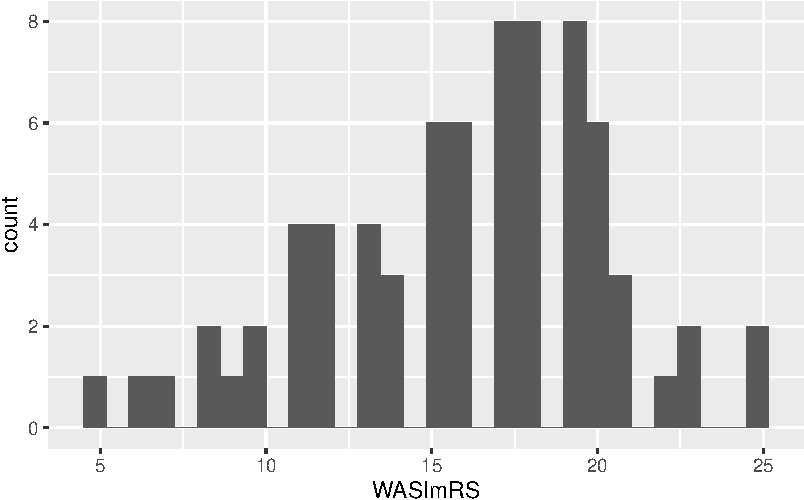
\includegraphics{visualization_files/figure-pdf/fig-hist-WASImRS-1.pdf}

}

\caption{\label{fig-hist-WASImRS}Distribution of WASImRS intelligence
scores}

\end{figure}

This is how the code works.

\begin{enumerate}
\def\labelenumi{\arabic{enumi}.}
\tightlist
\item
  \texttt{ggplot(data\ =\ conc.orth.subjs,\ ...} tells R what function
  to use \texttt{ggplot()} and what data to work with
  \texttt{data\ =\ conc.orth.subjs}.
\item
  \texttt{aes(x\ =\ WASImRS)} tells R what aesthetic mapping to use: we
  want to map values on the \texttt{WASImRS} variable (small to large)
  to locations on the x-axis (left to right).
\item
  \texttt{geom\_histogram()} tells R to construct a histogram,
  presenting a statistical summary of the distribution of intelligence
  scores.
\end{enumerate}

With histograms, we are visualizing the distribution of a single
continuous variable by dividing the variable values into bins
(i.e.~subsets) and counting the number of observations in each bin.
Histograms display the counts with bars.

You can see more information about \texttt{geom\_histogram}
\href{https://ggplot2.tidyverse.org/reference/geom_histogram.html}{here}.

Figure~\ref{fig-hist-WASImRS} shows how intelligence (WASImRS) scores
vary in the Ricketts Study 2 dataset. Scores peak around 17, with a long
tail of lower scores towards 5, and a maximum around 25.

Where I use the word ``peak'' I am talking about the tallest bar in the
plot (or, later the highest point in a density curve). At this point, we
have the most observations of the value under the bar. Here, we observed
the score WASImRS \(= 17\) for the most children in this sample.

A primary function of discovery visualization is to assess whether the
distribution of scores on a variable is consistent with expectations,
granted assumptions about a sample (e.g., that the children are
typically developing). We would normally use research area knowledge to
assess whether this distribution fits expectations for a sample of
typically developing school-aged children in the UK. However, I shall
leave that concern aside, here, so that we can focus on enriching the
plot presentation, next.

There are two main problems with the plot:

\begin{enumerate}
\def\labelenumi{\arabic{enumi}.}
\tightlist
\item
  The bars are ``gappy'' in the histogram, suggesting we have not
  grouped observed values in sufficiently wide subsets (bins). This is a
  problem because it weakens our ability to gain or communicate a visual
  sense of the distribution of scores.
\item
  The axis labeling uses the dataset variable name \texttt{WASImRS} but
  if we were to present the plot to others we could not expect them to
  know what that means.
\end{enumerate}

We can fix both these problems, and polish the plot for presentation,
through the following code steps.

\begin{Shaded}
\begin{Highlighting}[numbers=left,,]
\FunctionTok{ggplot}\NormalTok{(}\AttributeTok{data =}\NormalTok{ conc.orth.subjs, }\FunctionTok{aes}\NormalTok{(}\AttributeTok{x =}\NormalTok{ WASImRS)) }\SpecialCharTok{+}
  \FunctionTok{geom\_histogram}\NormalTok{(}\AttributeTok{binwidth =} \DecValTok{2}\NormalTok{) }\SpecialCharTok{+}
  \FunctionTok{labs}\NormalTok{(}\AttributeTok{x =} \StringTok{"Scores on the Wechsler Abbreviated Scale of Intelligence"}\NormalTok{) }\SpecialCharTok{+}
  \FunctionTok{theme\_bw}\NormalTok{()}
\end{Highlighting}
\end{Shaded}

\begin{figure}[H]

{\centering 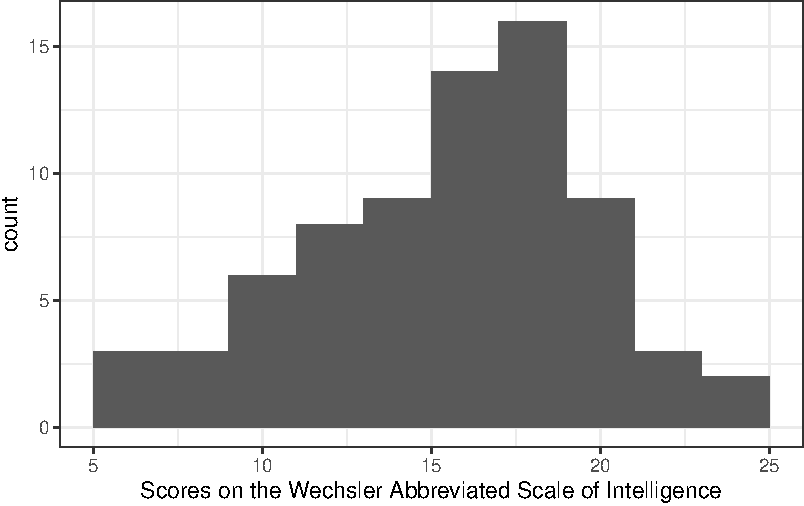
\includegraphics{visualization_files/figure-pdf/fig-hist-WASImRS-edits-1.pdf}

}

\caption{\label{fig-hist-WASImRS-edits}Distribution of WASImRS
intelligence scores}

\end{figure}

Figure~\ref{fig-hist-WASImRS-edits} shows the same data, and furnishes
us with the same picture of the distribution of intelligence scores but
it is a bit easier to read. We achieve this by making three edits.

\begin{enumerate}
\def\labelenumi{\arabic{enumi}.}
\tightlist
\item
  \texttt{geom\_histogram(binwidth\ =\ 2)\ +} we change the
  \texttt{binwidth}.
\end{enumerate}

\begin{itemize}
\tightlist
\item
  This is so that more different observed values of the data variable
  are included in bins (subsets corresponding to bars) so that the bars
  correspond to information about a wider range of values.
\item
  This makes the bars bigger, wider, and closes the gaps.
\item
  And this means we can focus the eyes of the audience for our plot on
  the visual impression we wish to communicate: the skewed distribution
  of intelligence scores.
\end{itemize}

\begin{enumerate}
\def\labelenumi{\arabic{enumi}.}
\setcounter{enumi}{1}
\tightlist
\item
  \texttt{labs(x\ =\ "Scores\ on\ the\ Wechsler\ Abbreviated\ Scale\ of\ Intelligence")\ +}
  changes the label to something that should be understandable by
  people, in our audience, who do not have access to variable
  information (as we do) about the dataset.
\item
  \texttt{theme\_bw()} we change the overall appearance of the plot by
  changing the theme.
\end{enumerate}

\hypertarget{exercise-1}{%
\subsubsection{Exercise}\label{exercise-1}}

We could, if we wanted, add a line and annotation to indicate the mean
value, as you saw in Figure~\ref{fig-sleep-study-histogram}.

\begin{itemize}
\tightlist
\item
  Can you add the necessary code to indicate the mean value of WASI
  scores, for this plot?
\end{itemize}

We can, of course, plot histograms to indicate the distributions of
other variables.

\begin{itemize}
\tightlist
\item
  Can you apply the histogram code to plot histograms of other
  variables?
\end{itemize}

\hypertarget{sec-compare-distributions}{%
\subsection{Comparing the distributions of numeric
variables}\label{sec-compare-distributions}}

We may wish to discover or communicate how values vary on dataset
variables in two different ways. Sometimes, we need to examine how
values vary on different variables. And sometimes, we need to examine
how values vary on the same variable but in different groups of
participants (or stimuli) or under different conditions. We look at this
next. We begin by looking at how you might compare how values vary on
different variables.

\hypertarget{sec-compare-distributions-variables}{%
\subsubsection{Compare how values vary on different
variables}\label{sec-compare-distributions-variables}}

It can be useful to compare the distributions of different variables.
Why?

Consider the Ricketts et al. (2021) investigation dataset. Like many
developmental investigations (see also clinical investigations), we
tested children and recorded their scores on a series of standardized
measures, here, measures of ability on a range of dimensions. We did
this, in part, to establish that the children in our sample are
operating at about the level one might expect for typically developing
children in cognitive ability dimensions of interest: dimensions like
intelligence, reading ability or spelling ability. So, one of the
aspects of the data we are considering is whether scores on these
dimensions are higher or lower than typical threshold levels. But we
also want to examine the distributions of scores because we want to find
out:

\begin{itemize}
\tightlist
\item
  if participants are varied in ability (wide distribution) or if maybe
  they are all similar (narrow distribution) as would be the case if the
  ability measures are too easy (so all scores are at ceiling) or too
  hard (so all scores are at floor);
\item
  if there are subgroups within the sample, maybe reflected by two or
  more peaks;
\item
  if there are unusual scores, maybe reflected by small peaks at very
  low or very high scores.
\end{itemize}

We could look at each variable, one plot at a time. Instead, next, I
will show you how to produce a set of histogram plots, and present them
all as a single grid of plots.

\begin{tcolorbox}[enhanced jigsaw, opacitybacktitle=0.6, title=\textcolor{quarto-callout-warning-color}{\faExclamationTriangle}\hspace{0.5em}{Warning}, arc=.35mm, colbacktitle=quarto-callout-warning-color!10!white, colframe=quarto-callout-warning-color-frame, leftrule=.75mm, opacityback=0, breakable, titlerule=0mm, left=2mm, bottomrule=.15mm, toprule=.15mm, colback=white, coltitle=black, bottomtitle=1mm, toptitle=1mm, rightrule=.15mm]

I have to warn you that the way I write the code is not good practice.
The code is written with repeats of the \texttt{ggplot()} block of code
to produce each plot. This repetition is inefficient and leaves the
coding vulnerable to errors because it is hard to spot a mistake in more
code. What I \emph{should} do is encapsulate the code as a function
(\href{https://r4ds.hadley.nz/functions.html}{see here}). The reason I
do not, here, is because I want to focus our attention on just the
plotting.

\end{tcolorbox}

Figure~\ref{fig-hist-grid} presents a grid of plots showing how scores
vary for each ability test measure, for the children in the Ricketts et
al. (2021) investigation dataset. We need to go through the code steps,
next, and discuss what the plots show us (discovery and communication).

\begin{Shaded}
\begin{Highlighting}[numbers=left,,]
\NormalTok{p.WASImRS }\OtherTok{\textless{}{-}} \FunctionTok{ggplot}\NormalTok{(}\AttributeTok{data =}\NormalTok{ conc.orth.subjs, }\FunctionTok{aes}\NormalTok{(}\AttributeTok{x =}\NormalTok{ WASImRS)) }\SpecialCharTok{+}
  \FunctionTok{geom\_histogram}\NormalTok{(}\AttributeTok{binwidth =} \DecValTok{2}\NormalTok{) }\SpecialCharTok{+}
  \FunctionTok{labs}\NormalTok{(}\AttributeTok{x =} \StringTok{"WASI matrix"}\NormalTok{) }\SpecialCharTok{+}
  \FunctionTok{theme\_bw}\NormalTok{()}

\NormalTok{p.TOWREsweRS }\OtherTok{\textless{}{-}} \FunctionTok{ggplot}\NormalTok{(}\AttributeTok{data =}\NormalTok{ conc.orth.subjs, }\FunctionTok{aes}\NormalTok{(}\AttributeTok{x =}\NormalTok{ TOWREsweRS)) }\SpecialCharTok{+}
  \FunctionTok{geom\_histogram}\NormalTok{(}\AttributeTok{binwidth =} \DecValTok{5}\NormalTok{) }\SpecialCharTok{+}
  \FunctionTok{labs}\NormalTok{(}\AttributeTok{x =} \StringTok{"TOWRE words"}\NormalTok{) }\SpecialCharTok{+}
  \FunctionTok{theme\_bw}\NormalTok{()}

\NormalTok{p.TOWREpdeRS }\OtherTok{\textless{}{-}} \FunctionTok{ggplot}\NormalTok{(}\AttributeTok{data =}\NormalTok{ conc.orth.subjs, }\FunctionTok{aes}\NormalTok{(}\AttributeTok{x =}\NormalTok{ TOWREpdeRS)) }\SpecialCharTok{+}
  \FunctionTok{geom\_histogram}\NormalTok{(}\AttributeTok{binwidth =} \DecValTok{5}\NormalTok{) }\SpecialCharTok{+}
  \FunctionTok{labs}\NormalTok{(}\AttributeTok{x =} \StringTok{"TOWRE phonemic"}\NormalTok{) }\SpecialCharTok{+}
  \FunctionTok{theme\_bw}\NormalTok{()}

\NormalTok{p.CC2regRS }\OtherTok{\textless{}{-}} \FunctionTok{ggplot}\NormalTok{(}\AttributeTok{data =}\NormalTok{ conc.orth.subjs, }\FunctionTok{aes}\NormalTok{(}\AttributeTok{x =}\NormalTok{ CC2regRS)) }\SpecialCharTok{+}
  \FunctionTok{geom\_histogram}\NormalTok{(}\AttributeTok{binwidth =} \DecValTok{2}\NormalTok{) }\SpecialCharTok{+}
  \FunctionTok{labs}\NormalTok{(}\AttributeTok{x =} \StringTok{"CC regular words"}\NormalTok{) }\SpecialCharTok{+}
  \FunctionTok{theme\_bw}\NormalTok{()}

\NormalTok{p.CC2irregRS }\OtherTok{\textless{}{-}} \FunctionTok{ggplot}\NormalTok{(}\AttributeTok{data =}\NormalTok{ conc.orth.subjs, }\FunctionTok{aes}\NormalTok{(}\AttributeTok{x =}\NormalTok{ CC2irregRS)) }\SpecialCharTok{+}
  \FunctionTok{geom\_histogram}\NormalTok{(}\AttributeTok{binwidth =} \DecValTok{2}\NormalTok{) }\SpecialCharTok{+}
  \FunctionTok{labs}\NormalTok{(}\AttributeTok{x =} \StringTok{"CC irregular words"}\NormalTok{) }\SpecialCharTok{+}
  \FunctionTok{theme\_bw}\NormalTok{()}

\NormalTok{p.CC2nwRS }\OtherTok{\textless{}{-}} \FunctionTok{ggplot}\NormalTok{(}\AttributeTok{data =}\NormalTok{ conc.orth.subjs, }\FunctionTok{aes}\NormalTok{(}\AttributeTok{x =}\NormalTok{ CC2nwRS)) }\SpecialCharTok{+}
  \FunctionTok{geom\_histogram}\NormalTok{(}\AttributeTok{binwidth =} \DecValTok{2}\NormalTok{) }\SpecialCharTok{+}
  \FunctionTok{labs}\NormalTok{(}\AttributeTok{x =} \StringTok{"CC nonwords"}\NormalTok{) }\SpecialCharTok{+}
  \FunctionTok{theme\_bw}\NormalTok{()}

\NormalTok{p.WASIvRS }\OtherTok{\textless{}{-}} \FunctionTok{ggplot}\NormalTok{(}\AttributeTok{data =}\NormalTok{ conc.orth.subjs, }\FunctionTok{aes}\NormalTok{(}\AttributeTok{x =}\NormalTok{ WASIvRS)) }\SpecialCharTok{+}
  \FunctionTok{geom\_histogram}\NormalTok{(}\AttributeTok{binwidth =} \DecValTok{2}\NormalTok{) }\SpecialCharTok{+}
  \FunctionTok{labs}\NormalTok{(}\AttributeTok{x =} \StringTok{"WASI vocabulary"}\NormalTok{) }\SpecialCharTok{+}
  \FunctionTok{theme\_bw}\NormalTok{()}

\NormalTok{p.BPVSRS }\OtherTok{\textless{}{-}} \FunctionTok{ggplot}\NormalTok{(}\AttributeTok{data =}\NormalTok{ conc.orth.subjs, }\FunctionTok{aes}\NormalTok{(}\AttributeTok{x =}\NormalTok{ BPVSRS)) }\SpecialCharTok{+}
  \FunctionTok{geom\_histogram}\NormalTok{(}\AttributeTok{binwidth =} \DecValTok{3}\NormalTok{) }\SpecialCharTok{+}
  \FunctionTok{labs}\NormalTok{(}\AttributeTok{x =} \StringTok{"BPVS vocabulary"}\NormalTok{) }\SpecialCharTok{+}
  \FunctionTok{theme\_bw}\NormalTok{()}

\NormalTok{p.mean.score }\OtherTok{\textless{}{-}} \FunctionTok{ggplot}\NormalTok{(}\AttributeTok{data =}\NormalTok{ conc.orth.subjs, }\FunctionTok{aes}\NormalTok{(}\AttributeTok{x =}\NormalTok{ mean.score)) }\SpecialCharTok{+}
  \FunctionTok{geom\_histogram}\NormalTok{(}\AttributeTok{binwidth =}\NormalTok{ .}\DecValTok{25}\NormalTok{) }\SpecialCharTok{+}
  \FunctionTok{labs}\NormalTok{(}\AttributeTok{x =} \StringTok{"Mean orthographic test score"}\NormalTok{) }\SpecialCharTok{+}
  \FunctionTok{theme\_bw}\NormalTok{()}

\NormalTok{p.mean.score }\SpecialCharTok{+}\NormalTok{ p.BPVSRS }\SpecialCharTok{+}\NormalTok{ p.WASIvRS }\SpecialCharTok{+}\NormalTok{ p.WASImRS }\SpecialCharTok{+}
\NormalTok{  p.CC2nwRS }\SpecialCharTok{+}\NormalTok{ p.CC2irregRS }\SpecialCharTok{+}\NormalTok{ p.CC2regRS }\SpecialCharTok{+} 
\NormalTok{  p.TOWREpdeRS }\SpecialCharTok{+}\NormalTok{ p.TOWREsweRS }\SpecialCharTok{+} \FunctionTok{plot\_layout}\NormalTok{(}\AttributeTok{ncol =} \DecValTok{3}\NormalTok{)}
\end{Highlighting}
\end{Shaded}

\begin{figure}[H]

{\centering 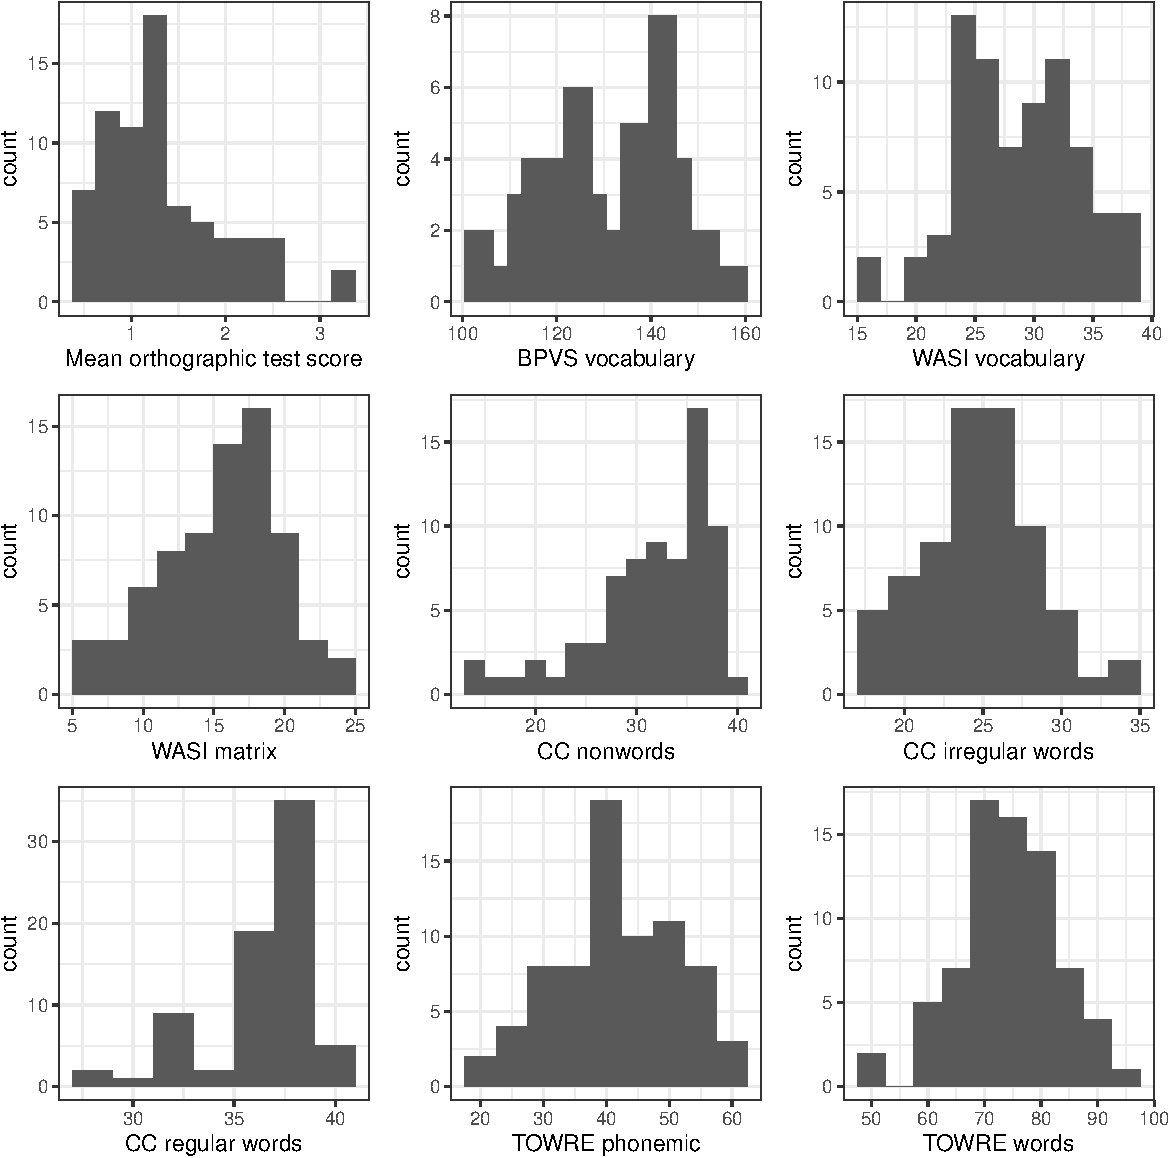
\includegraphics{visualization_files/figure-pdf/fig-hist-grid-1.pdf}

}

\caption{\label{fig-hist-grid}Distribution of childrens' scores on
ability measures}

\end{figure}

This is how the code works, step by step:

\begin{enumerate}
\def\labelenumi{\arabic{enumi}.}
\tightlist
\item
  \texttt{p.WASImRS\ \textless{}-\ ggplot(...)} first creates a plot
  object, which we call \texttt{p.WASImRS}.
\item
  \texttt{ggplot(data\ =\ conc.orth.subjs,\ aes(x\ =\ WASImRS))\ +}
  tells R what data to use, and what aesthetic mapping to work with
  mapping the variable \texttt{WASImRS} here to the x-axis location.
\item
  \texttt{geom\_histogram(binwidth\ =\ 2)\ +} tells R to sort the values
  of \texttt{WASImRS} scores into bins and create a histogram to show
  how many children in the sample present scores of different sizes.
\item
  \texttt{labs(x\ =\ "WASI\ matrix")\ +} changes the x-axis label to
  make it more informative.
\item
  \texttt{theme\_bw()} changes the theme to make it a bit cleaner
  looking.
\end{enumerate}

We do this bit of code separately for each variable. We change the plot
object name, the \texttt{x\ =} variable specification, and the axis
label text for each variable. We adjust the binwidth where it appears to
be necessary.

We then use the following plot code to put all the plots together in a
single grid.

\begin{Shaded}
\begin{Highlighting}[]
\NormalTok{p.mean.score }\SpecialCharTok{+}\NormalTok{ p.BPVSRS }\SpecialCharTok{+}\NormalTok{ p.WASIvRS }\SpecialCharTok{+}\NormalTok{ p.WASImRS }\SpecialCharTok{+}
\NormalTok{  p.CC2nwRS }\SpecialCharTok{+}\NormalTok{ p.CC2irregRS }\SpecialCharTok{+}\NormalTok{ p.CC2regRS }\SpecialCharTok{+} 
\NormalTok{  p.TOWREpdeRS }\SpecialCharTok{+}\NormalTok{ p.TOWREsweRS }\SpecialCharTok{+} \FunctionTok{plot\_layout}\NormalTok{(}\AttributeTok{ncol =} \DecValTok{3}\NormalTok{)}
\end{Highlighting}
\end{Shaded}

\begin{itemize}
\tightlist
\item
  In the code, we add a series of plots together
  e.g.~\texttt{p.mean.score\ +\ p.BPVSRS\ +\ p.WASIvRS\ ...}
\item
  and then specify we want a grid of plots with a layout of three
  columns \texttt{plot\_layout(ncol\ =\ 3)}.
\end{itemize}

This syntax requires the \texttt{library(patchwork)} and more
information about this very useful library can be found
\href{https://patchwork.data-imaginist.com}{here}.

What do the plots show us?

Figure~\ref{fig-hist-grid} shows a grid of 9 histogram plots. Each plot
presents the distribution of scores for the Ricketts et al. (2021) Study
2 participant sample on a separate ability measure, including scores on
the BPVS vocabulary, WASI vocabulary, TOWRE words and TOWRE nonwords
reading tests, as well as scores on the Castles and Coltheart regular
words, irregular words and nonwords reading tests, and the mean
Levenshtein distance (spelling score) outcome measure of performance for
the experimental word learning post-test.

Take a look, you may notice the following features.

\begin{enumerate}
\def\labelenumi{\arabic{enumi}.}
\tightlist
\item
  The mean orthographic test score suggests that many children produced
  spellings to the words they learned in the Ricketts et al. (2021)
  study that, on average, were correct (0 edits) or were one or two
  edits (e.g., a letter deletion or replacement) away from the target
  word spelling. The children were learning the words, and most of the
  time, they learned the spellings of the words effectively. However,
  one or two children tended to produce spellings that were 2-3 edits
  distant from the target spelling.
\end{enumerate}

\begin{itemize}
\tightlist
\item
  We can see these features because we can see that the histogram peaks
  around 1 (at Levenshtein distance score \(= 1\)) but that there is a
  small bar of scores at around 3.
\end{itemize}

\begin{enumerate}
\def\labelenumi{\arabic{enumi}.}
\setcounter{enumi}{1}
\tightlist
\item
  We can see that there are two peaks on the BPVS and WASI measures of
  vocabulary. What is going on there?
\end{enumerate}

\begin{itemize}
\tightlist
\item
  Is it the case that we have two sub-groups of children within the
  overall sample? For example, on the BPVS test, maybe one sub-group of
  children has a distribution of vocabulary scores with a peak around
  120 (the peak shows where most children have scores) while another
  sub-group of children has a distribution of vocabulary scores with a
  peak around 140.
\end{itemize}

\begin{enumerate}
\def\labelenumi{\arabic{enumi}.}
\setcounter{enumi}{2}
\tightlist
\item
  If we look at the CC nonwords and CC regular words tests of reading
  ability, we may notice that while most children present relatively
  high scores on these tests (CC nonwords peak around 35, CC regular
  words peak around 37) there is a skewed distribution. Many of the
  children's scores are piled up towards the maximum value in the data
  on the measures. But we can also see that, on both measures, there are
  long tails in the distributions because relatively small numbers of
  children have substantially lower scores.
\end{enumerate}

\begin{itemize}
\tightlist
\item
  Developmental samples are often highly varied (just like clinical
  samples). Are all the children in the sample at the same developmental
  stage, or are they all typically developing?
\end{itemize}

\begin{tcolorbox}[enhanced jigsaw, opacitybacktitle=0.6, title=\textcolor{quarto-callout-tip-color}{\faLightbulb}\hspace{0.5em}{Tip}, arc=.35mm, colbacktitle=quarto-callout-tip-color!10!white, colframe=quarto-callout-tip-color-frame, leftrule=.75mm, opacityback=0, breakable, titlerule=0mm, left=2mm, bottomrule=.15mm, toprule=.15mm, colback=white, coltitle=black, bottomtitle=1mm, toptitle=1mm, rightrule=.15mm]

Notice that in presenting a grid of plots like this, we offer a compact
visual way to present the same summary information we might otherwise
present using a table of descriptive statistics. In some ways, this grid
of plots is more informative than the descriptive statistics because the
mean and SD values do not tell you what you can see:

\begin{itemize}
\tightlist
\item
  the characteristics of the variation in values, like the presence of
  two peaks;
\item
  or the presence of unusually high or low scores (for this sample).
\end{itemize}

\end{tcolorbox}

Grids of plots like this can be helpful to inspect the distributions of
variables in a concise approach. They are not really too useful for
\emph{comparing} the distributions because they require your eyes to
move between plots, repeatedly, to do the comparison.

Here is a more compact way to code the grid of histograms using the
\texttt{library(ggridges)} function \texttt{geom\_density\_ridges()}. I
do not discuss it in detail because I want to focus your attention on
core \texttt{tidyverse} functions (I show you more information in the
\texttt{Notes} tab).

Notice that if you produce all the plots so that the are in line in the
same column with a shared x-axis it becomes \emph{much easier} to
compare the distributions of scores. You lose some of the fine detail,
discussed in relation to Figure~\ref{fig-hist-grid}, but this style
allows you to gain an impression, quickly, of how for distributions of
scores compare between measures. For example, we can see that within the
Castles and Coltheart (CC) measures of reading ability, children do
better on regular words than on nonwords, and on nonwords better than on
irregular words.

\section{Plot}

\begin{Shaded}
\begin{Highlighting}[numbers=left,,]
\FunctionTok{library}\NormalTok{(ggridges)}
\NormalTok{conc.orth.subjs }\SpecialCharTok{\%\textgreater{}\%}
  \FunctionTok{pivot\_longer}\NormalTok{(}\AttributeTok{names\_to =} \StringTok{"task"}\NormalTok{, }\AttributeTok{values\_to =} \StringTok{"score"}\NormalTok{, }\AttributeTok{cols =}\NormalTok{ WASImRS}\SpecialCharTok{:}\NormalTok{mean.score) }\SpecialCharTok{\%\textgreater{}\%} 
  \FunctionTok{ggplot}\NormalTok{(}\FunctionTok{aes}\NormalTok{(}\AttributeTok{y =}\NormalTok{ task, }\AttributeTok{x =}\NormalTok{ score)) }\SpecialCharTok{+}
  \FunctionTok{geom\_density\_ridges}\NormalTok{(}\AttributeTok{stat =} \StringTok{"binline"}\NormalTok{, }\AttributeTok{bins =} \DecValTok{20}\NormalTok{, }\AttributeTok{scale =} \FloatTok{0.95}\NormalTok{, }\AttributeTok{draw\_baseline =} \ConstantTok{FALSE}\NormalTok{) }\SpecialCharTok{+}
  \FunctionTok{theme\_ridges}\NormalTok{()}
\end{Highlighting}
\end{Shaded}

\begin{figure}[H]

{\centering 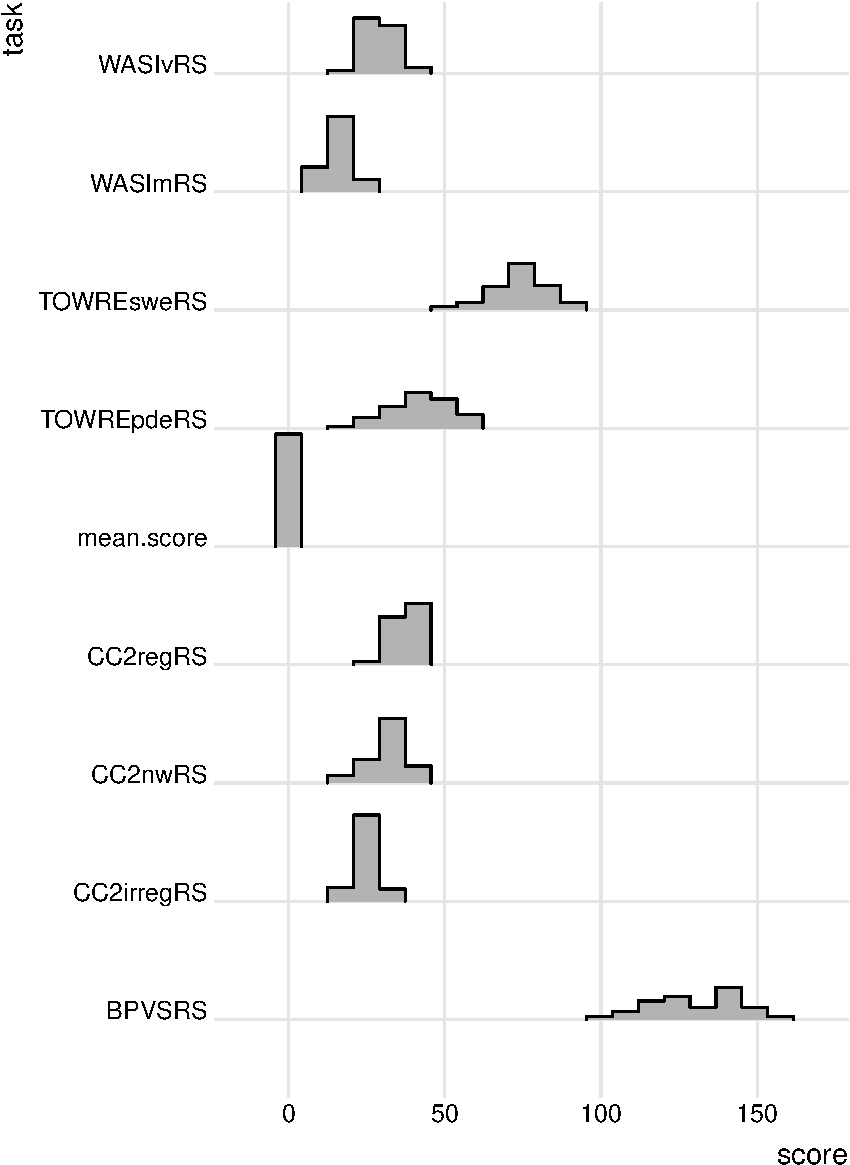
\includegraphics{visualization_files/figure-pdf/fig-ridges-grid-1.pdf}

}

\caption{\label{fig-ridges-grid}Distribution of childrens' scores on
ability measures}

\end{figure}

\section{Notes}

\begin{enumerate}
\def\labelenumi{\arabic{enumi}.}
\tightlist
\item
  \texttt{library(ggridges)} get the library we need.
\item
  \texttt{conc.orth.subjs\ \%\textgreater{}\%} pipe the dataset for
  processing.
\item
  \texttt{pivot\_longer(names\_to\ =\ "task",\ values\_to\ =\ "score",\ cols\ =\ WASImRS:mean.score)\ \%\textgreater{}\%}
  pivot the data so all test scores are in the same column, ``scores''
  wwith coding for ``task'' name, and pipe to the next step for
  plotting.
\item
  \texttt{ggplot(aes(y\ =\ task,\ x\ =\ score))\ +} create a plot for
  the scores on each task.
\item
  \texttt{geom\_density\_ridges(stat\ =\ "binline",\ bins\ =\ 20,\ scale\ =\ 0.95,\ draw\_baseline\ =\ FALSE)\ +}
  show the plots as histograms.
\item
  \texttt{theme\_ridges()} change the theme to the specific theme
  suitable for showing a grid of ridges.
\end{enumerate}

You can find more information on \texttt{ggridges}
\href{https://cran.r-project.org/web/packages/ggridges/vignettes/introduction.html}{here}.

\hypertarget{sec-compare-distributions-groups}{%
\subsubsection{Compare between groups how values vary on different
variables}\label{sec-compare-distributions-groups}}

We will often want to compare the distributions of variable values
between groups or between conditions. This need may appear when, for
example, we are conducting a between-groups manipulation of some
condition and we want to check that the groups are approximately matched
on dimensions that are potentially linked to outcomes (i.e., on
potential \emph{confounds}). The need may appear when, alternatively, we
have recruited or selected participant (or stimulus) samples and we want
to check that the sample sub-groups are approximately matched or
detectably different on one or more dimensions of interest or of
concern.

As a demonstration of the visualization work we can do in such contexts,
let's pick up on an observation we made earlier, that there are two
peaks on the BPVS and WASI measures of vocabulary. I asked: Is it the
case that we have two sub-groups of children within the overall sample?
Actually, we know the answer to that question because Ricketts et al.
(2021) state that they recruited one set of children for their Study 1
and then, for Study 2:

\begin{quote}
Thirty-three children from an additional three socially mixed schools in
the South-East of England were added to the Study 1 sample (total N =
74). These additional children were older (\(M_{age}\) = 12.57, SD =
0.29, 17 female)
\end{quote}

Do the younger (Study 1) children differ in any way from the older
(additional) children?

We can check this through data visualization. Our aim is to present the
distributions of variables side-by-side or \emph{superimposed} to ensure
easy comparison. We can do this in different ways, so I will demonstrate
one approach with an outline explanation of the actions, and offer
suggestions for further approaches.

I am going to process the data before I do the plotting. I will re-use
the code I used before (see Section~\ref{sec-get-distinct}) with one
additional change. I will add a line to create a group coding variable.
This addition shows you how to do an action that is \emph{very often}
useful in the data processing part of your workflow.

\hypertarget{sec-process-code-group}{%
\paragraph{Data processing}\label{sec-process-code-group}}

You have seen that the Ricketts et al. (2021) report states that an
additional group of children was recruited for the investigation's
second study. How do we know who they are? If you recall the summary
view of the complete dataset, there is one variable we can use to code
group identity.

\begin{Shaded}
\begin{Highlighting}[]
\FunctionTok{summary}\NormalTok{(conc.orth}\SpecialCharTok{$}\NormalTok{Study)}
\end{Highlighting}
\end{Shaded}

\begin{verbatim}
Study1&2   Study2 
     655      512 
\end{verbatim}

This summary tells us that we have 512 observations concerning the
additional group of children recruited for \texttt{Study\ 2}, and 655
observations for the (younger) children whose data were analyzed for
both Study 1 and Study 2 (i.e., coded as \texttt{Study1\&2} in the
\texttt{Study} variable column). We can use this information to create a
coding variable. (If we had age data, we could use that instead but we
do not.) This is how we do that.

\begin{Shaded}
\begin{Highlighting}[]
\NormalTok{conc.orth.subjs }\OtherTok{\textless{}{-}}\NormalTok{ conc.orth }\SpecialCharTok{\%\textgreater{}\%}
  \FunctionTok{group\_by}\NormalTok{(Participant) }\SpecialCharTok{\%\textgreater{}\%}
  \FunctionTok{mutate}\NormalTok{(}\AttributeTok{mean.score =} \FunctionTok{mean}\NormalTok{(Levenshtein.Score)) }\SpecialCharTok{\%\textgreater{}\%}
  \FunctionTok{ungroup}\NormalTok{() }\SpecialCharTok{\%\textgreater{}\%}
  \FunctionTok{distinct}\NormalTok{(Participant, }\AttributeTok{.keep\_all =} \ConstantTok{TRUE}\NormalTok{) }\SpecialCharTok{\%\textgreater{}\%}
  \FunctionTok{mutate}\NormalTok{(}\AttributeTok{age.group =} \FunctionTok{fct\_recode}\NormalTok{(Study,}
    
    \StringTok{"young"} \OtherTok{=} \StringTok{"Study1\&2"}\NormalTok{,}
    \StringTok{"old"} \OtherTok{=} \StringTok{"Study2"}
    
\NormalTok{  )) }\SpecialCharTok{\%\textgreater{}\%}
  \FunctionTok{select}\NormalTok{(WASImRS}\SpecialCharTok{:}\NormalTok{BPVSRS, mean.score, Participant, age.group)}
\end{Highlighting}
\end{Shaded}

The code block is mostly the same as the code I used in Section
Section~\ref{sec-get-distinct} to extract the data for each participant,
with two changes:

\begin{enumerate}
\def\labelenumi{\arabic{enumi}.}
\tightlist
\item
  First, \texttt{mutate(age.group\ =\ fct\_recode(...)} tells R that I
  want to create a new variable \texttt{age.group} through the process
  of recoding, with \texttt{fct\_recode(...)} the variable I specify
  next, in the way that I specify.
\item
  \texttt{fct\_recode(Study,\ ...)} tells R I want to recode the
  variable \texttt{Study}.
\item
  \texttt{"young"\ =\ "Study1\&2",\ "old"\ =\ "Study2"} specifies what I
  want recoded.
\end{enumerate}

\begin{itemize}
\tightlist
\item
  I am telling R to look in the \texttt{Study} column and (a.) whenever
  it finds the value \texttt{Study1\&2} replace it with \texttt{young}
  whereas (b.) whenever it finds the value \texttt{Study2} replace it
  with \texttt{old}.
\item
  Notice that the syntax in recoding is \texttt{fct\_recode}: ``new
  name'' = ``old name''.
\item
  Having done that, I tell R to pipe the data, including the recoded
  variable, to the next step.
\end{itemize}

\begin{enumerate}
\def\labelenumi{\arabic{enumi}.}
\setcounter{enumi}{3}
\tightlist
\item
  \texttt{select(WASImRS:BPVSRS,\ mean.score,\ Participant,\ age.group)}
  where I add the new recoded variable to the selection of variables I
  want to include in the new dataset \texttt{conc.orth.subjs}.
\end{enumerate}

\begin{tcolorbox}[enhanced jigsaw, opacitybacktitle=0.6, title=\textcolor{quarto-callout-tip-color}{\faLightbulb}\hspace{0.5em}{Tip}, arc=.35mm, colbacktitle=quarto-callout-tip-color!10!white, colframe=quarto-callout-tip-color-frame, leftrule=.75mm, opacityback=0, breakable, titlerule=0mm, left=2mm, bottomrule=.15mm, toprule=.15mm, colback=white, coltitle=black, bottomtitle=1mm, toptitle=1mm, rightrule=.15mm]

Notice that R handles categorical or nominal variables like
\texttt{Study} (or, in other data, variables e.g.~gender, education or
ethnicity) as \emph{factors}.

\begin{itemize}
\tightlist
\item
  Within a classification scheme like education, we may have different
  classes or categories or groups e.g.~``further, higher, school''. We
  can code these different classes with numbers (e.g.~\(school = 1\)) or
  with words ``further, higher, school''. Whatever we use, the different
  classes or groups are referred to as \emph{levels} and each level has
  a name.
\item
  In factor recoding, we are \emph{changing level names} while keeping
  the underlying data the same.
\end{itemize}

\end{tcolorbox}

The \texttt{tidyverse} collection includes the \texttt{forcats} library
of functions for working with categorical variables
(\texttt{forcats\ =\ factors}). These functions are often very useful
and you can read more about them
\href{https://forcats.tidyverse.org}{here}.

Changing factors level coding by hand is, for many, a common task, and
the \texttt{fct\_recode()} function makes it easy. You can find the
technical information on the function, with further examples,
\href{https://forcats.tidyverse.org/reference/fct_recode.html}{here}.

\hypertarget{sec-group-compare-distribution}{%
\paragraph{Group comparison
visualization}\label{sec-group-compare-distribution}}

There are different ways to examine the distributions of variables
\emph{so that} we can compare the distributions of the same variable
between groups.

Figure~\ref{fig-distribution-comparison-grid} presents some alternatives
as a grid of 4 different kinds of plots designed to enable the same
comparison. Each plot presents the distribution of scores for the
Ricketts et al. (2021) Study 2 participant sample on the BPVS vocabulary
measure so that we can compare the distribution of vocabulary scores
between age groups.

The plots differ in method using:

\begin{enumerate}
\def\labelenumi{\alph{enumi}.}
\tightlist
\item
  facetted histograms showing the distribution of vocabulary scores,
  separately for each group, in side-by-side histograms for comparison;
\item
  boxplots, showing the distribution of scores for each group, indicated
  by the y-axis locations of the edges of the boxes (25\% and 75\%
  quartiles) and the middle lines (medians);
\item
  superimposed histograms, where the histograms for the separate groups
  are laid on top of each other but given different colours to allow
  comparison; and
\item
  superimposed density plots where the densities for the separate groups
  are laid on top of each other but given different colours to allow
  comparison.
\end{enumerate}

\begin{tcolorbox}[enhanced jigsaw, opacitybacktitle=0.6, title=\textcolor{quarto-callout-tip-color}{\faLightbulb}\hspace{0.5em}{Tip}, arc=.35mm, colbacktitle=quarto-callout-tip-color!10!white, colframe=quarto-callout-tip-color-frame, leftrule=.75mm, opacityback=0, breakable, titlerule=0mm, left=2mm, bottomrule=.15mm, toprule=.15mm, colback=white, coltitle=black, bottomtitle=1mm, toptitle=1mm, rightrule=.15mm]

There is one thing you should notice about all these plots.

\begin{itemize}
\tightlist
\item
  It looks like the BPVS vocabulary scores have their peak -- most
  children show this value -- at around 120 for the \texttt{young} group
  and at around 140 for the \texttt{old} group.\\
\item
  We return to this shortly.
\end{itemize}

\end{tcolorbox}

I am going to hide the coding and the explanation of the coding behind
the \texttt{Notes} tab. Click on the tab to get a step-by-step
explanation. Of these alternatives, I focus on one which I explain in
more depth, following: d.~Superimposed density plots.

\section{Plot}

\begin{figure}

{\centering 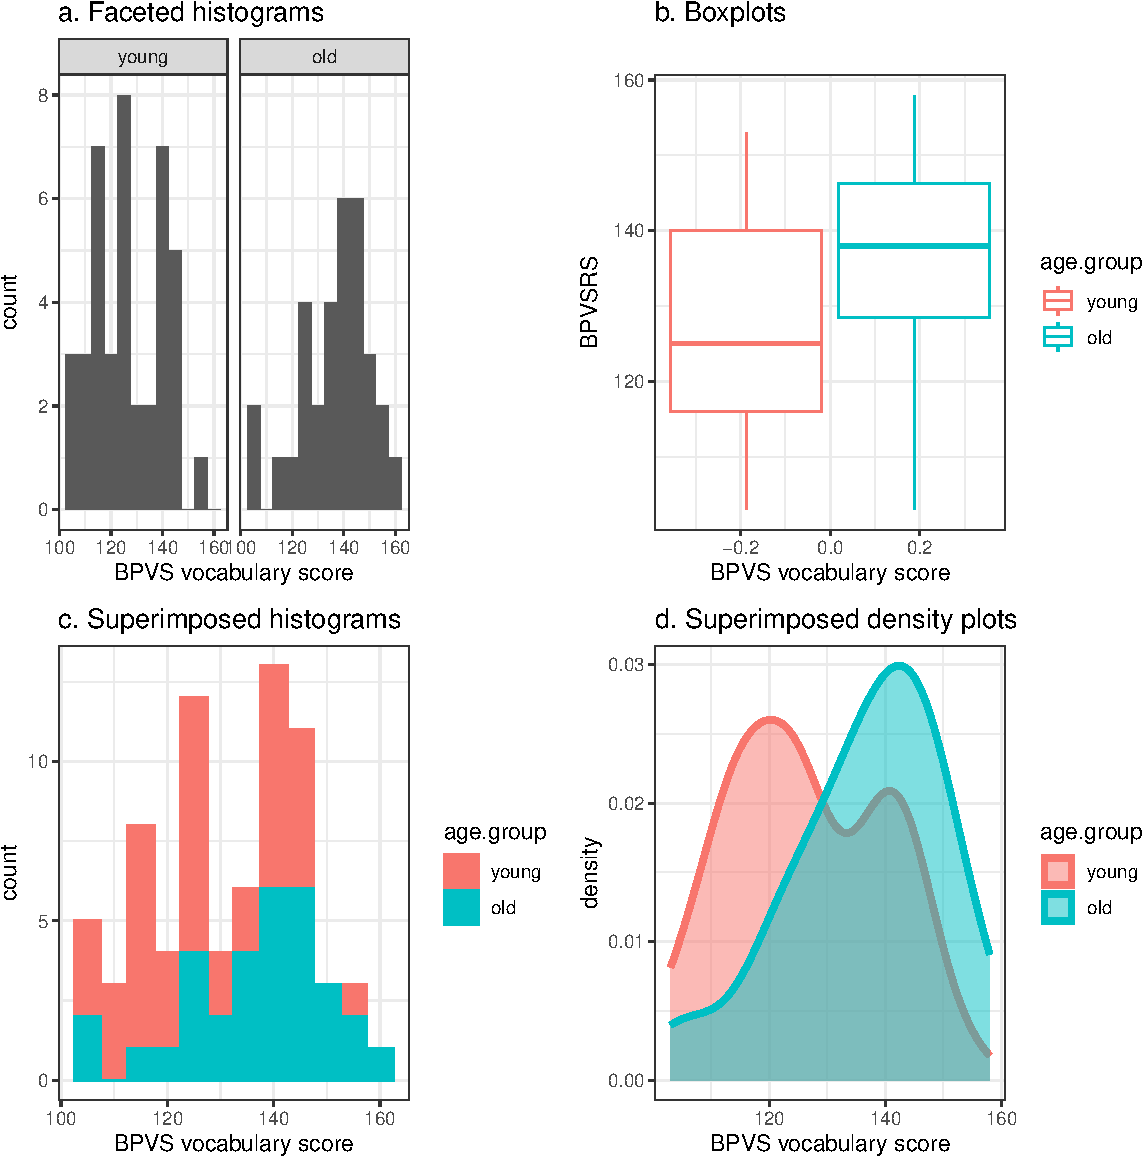
\includegraphics{visualization_files/figure-pdf/fig-distribution-comparison-grid-1.pdf}

}

\caption{\label{fig-distribution-comparison-grid}Distribution of
childrens' scores on the BPVS vocabulary measure: distributions are
compared between the younger and older age groups}

\end{figure}

\section{Notes}

\begin{Shaded}
\begin{Highlighting}[]
\NormalTok{p.facet.hist }\OtherTok{\textless{}{-}} \FunctionTok{ggplot}\NormalTok{(}\AttributeTok{data =}\NormalTok{ conc.orth.subjs, }\FunctionTok{aes}\NormalTok{(}\AttributeTok{x =}\NormalTok{ BPVSRS)) }\SpecialCharTok{+}
  \FunctionTok{geom\_histogram}\NormalTok{(}\AttributeTok{binwidth =} \DecValTok{5}\NormalTok{) }\SpecialCharTok{+}
  \FunctionTok{labs}\NormalTok{(}\AttributeTok{x =} \StringTok{"BPVS vocabulary score"}\NormalTok{, }\AttributeTok{title =} \StringTok{"a. Faceted histograms"}\NormalTok{) }\SpecialCharTok{+}
  \FunctionTok{facet\_wrap}\NormalTok{(}\SpecialCharTok{\textasciitilde{}}\NormalTok{ age.group) }\SpecialCharTok{+}
  \FunctionTok{theme\_bw}\NormalTok{()}

\NormalTok{p.colour.boxplot }\OtherTok{\textless{}{-}} \FunctionTok{ggplot}\NormalTok{(}\AttributeTok{data =}\NormalTok{ conc.orth.subjs, }\FunctionTok{aes}\NormalTok{(}\AttributeTok{y =}\NormalTok{ BPVSRS, }\AttributeTok{colour =}\NormalTok{ age.group)) }\SpecialCharTok{+}
  \FunctionTok{geom\_boxplot}\NormalTok{() }\SpecialCharTok{+}
  \FunctionTok{labs}\NormalTok{(}\AttributeTok{x =} \StringTok{"BPVS vocabulary score"}\NormalTok{, }\AttributeTok{title =} \StringTok{"b. Boxplots"}\NormalTok{) }\SpecialCharTok{+}
  \FunctionTok{theme\_bw}\NormalTok{()}

\NormalTok{p.colour.hist }\OtherTok{\textless{}{-}} \FunctionTok{ggplot}\NormalTok{(}\AttributeTok{data =}\NormalTok{ conc.orth.subjs, }\FunctionTok{aes}\NormalTok{(}\AttributeTok{x =}\NormalTok{ BPVSRS, }\AttributeTok{colour =}\NormalTok{ age.group, }\AttributeTok{fill =}\NormalTok{ age.group)) }\SpecialCharTok{+}
  \FunctionTok{geom\_histogram}\NormalTok{(}\AttributeTok{binwidth =} \DecValTok{5}\NormalTok{) }\SpecialCharTok{+}
  \FunctionTok{labs}\NormalTok{(}\AttributeTok{x =} \StringTok{"BPVS vocabulary score"}\NormalTok{, }\AttributeTok{title =} \StringTok{"c. Superimposed histograms"}\NormalTok{) }\SpecialCharTok{+}
  \FunctionTok{theme\_bw}\NormalTok{()}

\NormalTok{p.colour.density }\OtherTok{\textless{}{-}} \FunctionTok{ggplot}\NormalTok{(}\AttributeTok{data =}\NormalTok{ conc.orth.subjs, }\FunctionTok{aes}\NormalTok{(}\AttributeTok{x =}\NormalTok{ BPVSRS, }\AttributeTok{colour =}\NormalTok{ age.group, }\AttributeTok{fill =}\NormalTok{ age.group)) }\SpecialCharTok{+}
  \FunctionTok{geom\_density}\NormalTok{(}\AttributeTok{alpha =}\NormalTok{ .}\DecValTok{5}\NormalTok{, }\AttributeTok{size =} \FloatTok{1.5}\NormalTok{) }\SpecialCharTok{+}
  \FunctionTok{labs}\NormalTok{(}\AttributeTok{x =} \StringTok{"BPVS vocabulary score"}\NormalTok{, }\AttributeTok{title =} \StringTok{"d. Superimposed density plots"}\NormalTok{) }\SpecialCharTok{+}
  \FunctionTok{theme\_bw}\NormalTok{()}

\NormalTok{p.facet.hist }\SpecialCharTok{+}\NormalTok{ p.colour.boxplot }\SpecialCharTok{+}\NormalTok{ p.colour.hist }\SpecialCharTok{+}\NormalTok{ p.colour.density}
\end{Highlighting}
\end{Shaded}

\begin{enumerate}
\def\labelenumi{\arabic{enumi}.}
\tightlist
\item
  In plot ``a. Faceted histograms'', we use the code to construct a
  histogram but the difference is we use:
\end{enumerate}

\begin{itemize}
\tightlist
\item
  \texttt{facet\_wrap(\textasciitilde{}\ age.group)} to tell R to split
  the data by \texttt{age.group} then present the histograms indicating
  vocabulary score distributions \emph{separately} for each group.
\end{itemize}

\begin{enumerate}
\def\labelenumi{\arabic{enumi}.}
\setcounter{enumi}{1}
\tightlist
\item
  In plot ``b. Boxplots'', we use the \texttt{geom\_boxplot()} code to
  construct a boxplot to summarize the distributions of vocabulary
  scores -- as you have seen previously -- but the difference is we use:
\end{enumerate}

\begin{itemize}
\tightlist
\item
  \texttt{aes(y\ =\ BPVSRS,\ colour\ =\ age.group)} to tell R to assign
  different colours to different levels of \texttt{age.group} to help
  distinguish the data from each group.
\end{itemize}

\begin{enumerate}
\def\labelenumi{\arabic{enumi}.}
\setcounter{enumi}{2}
\tightlist
\item
  In plot ``c.~Superimposed histograms'', we use the code to construct a
  histogram but the difference is we use:
\end{enumerate}

\begin{itemize}
\tightlist
\item
  \texttt{aes(x\ =\ BPVSRS,\ colour\ =\ age.group,\ fill\ =\ age.group)}
  to tell R to assign different colours to different levels of
  \texttt{age.group} to help distinguish the data from each group.
\item
  Notice that the \texttt{fill} gives the colour inside the bars and
  \texttt{colour} gives the colour of the outline edges of the bars.
\end{itemize}

\begin{enumerate}
\def\labelenumi{\arabic{enumi}.}
\setcounter{enumi}{3}
\tightlist
\item
  In plot ``d.~Superimposed density plots'', we use the code
  \texttt{geom\_density(...)} to construct what is called a density
  plot.
\end{enumerate}

\begin{itemize}
\tightlist
\item
  A density plot presents a smoothed histogram to show the distribution
  of variable values.
\item
  We add arguments in
  \texttt{geom\_density(alpha\ =\ .5,\ size\ =\ 1.5)} to adjust the
  thickness of the line (\texttt{size\ =\ 1.5}) drawn to show the shape
  of the distribution and adjust the transparency of the colour fill
  inside the line \texttt{alpha\ =\ .5}).
\item
  We
  use\texttt{aes(x\ =\ BPVSRS,\ colour\ =\ age.group,\ fill\ =\ age.group)}
  to tell R to assign different colours to different levels of
  \texttt{age.group} to help distinguish the data from each group.
\item
  Notice that the \texttt{fill} gives the colour inside the density
  plots and \texttt{colour} gives the colour of the outline edges of the
  densities.
\end{itemize}

Density plots can be helpful when we wish to compare distributions. This
is because we can \emph{superimpose} distribution plots on top of each
other, enabling us or our audience to directly compare the
distributions: \emph{directly} because the distributions are shown on
the same scale, in the same image.

We can (roughly) understand a density plot as working like a smoothed
version of the histogram. Imagine how the heights of the bars in the
histogram represent how many observations we have of the values in a
particular bin. If we draw a smooth curving line through the tops of the
bars then we are representing the chances that an observation in our
sample has a value (the value under the curve) at any specific location
on the x-axis. You can see that in
Figure~\ref{fig-density-demonstration}.

\begin{verbatim}
Warning: The dot-dot notation (`..density..`) was deprecated in ggplot2 3.4.0.
i Please use `after_stat(density)` instead.
\end{verbatim}

\begin{figure}

{\centering 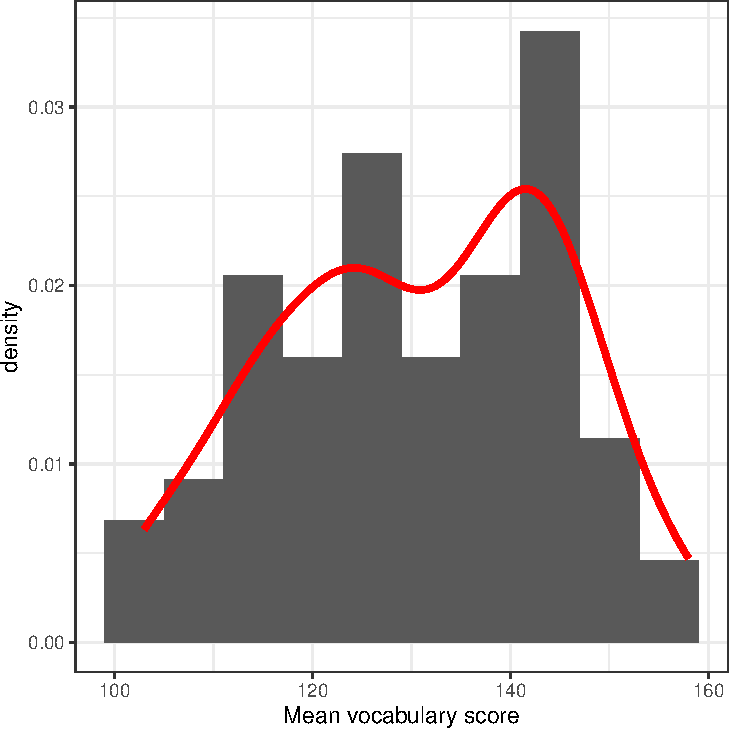
\includegraphics{visualization_files/figure-pdf/fig-density-demonstration-1.pdf}

}

\caption{\label{fig-density-demonstration}Distribution of childrens'
scores on the BPVS vocabulary measure. The figure shows the histogram
versus density plot representation of the same data distribution}

\end{figure}

You can find the \texttt{ggplot2} reference information on the
\texttt{geom\_density()} function, with further examples,
\href{https://ggplot2.tidyverse.org/reference/geom_density.html}{here}.
You can find technical information on density functions
\href{https://stackoverflow.com/questions/12394321/r-what-algorithm-does-geom-density-use-and-how-to-extract-points-equation-of}{here}
and
\href{https://en.wikipedia.org/wiki/Kernel_density_estimation}{here}.

We can develop the density plot to enrich the information we can
discover or communicate through the plot.
Figure~\ref{fig-density-BPVS-WASI} shows the distribution of scores on
both the BPVS and WASI vocabulary knowledge measures.

\begin{Shaded}
\begin{Highlighting}[numbers=left,,]
\NormalTok{p.BPVSRS.density }\OtherTok{\textless{}{-}} \FunctionTok{ggplot}\NormalTok{(}\AttributeTok{data =}\NormalTok{ conc.orth.subjs, }\FunctionTok{aes}\NormalTok{(}\AttributeTok{x =}\NormalTok{ BPVSRS, }\AttributeTok{colour =}\NormalTok{ age.group, }\AttributeTok{fill =}\NormalTok{ age.group)) }\SpecialCharTok{+}
  \FunctionTok{geom\_density}\NormalTok{(}\AttributeTok{alpha =}\NormalTok{ .}\DecValTok{5}\NormalTok{, }\AttributeTok{size =} \FloatTok{1.5}\NormalTok{) }\SpecialCharTok{+}
  \FunctionTok{geom\_rug}\NormalTok{(}\AttributeTok{alpha =}\NormalTok{ .}\DecValTok{5}\NormalTok{) }\SpecialCharTok{+}
  \FunctionTok{geom\_vline}\NormalTok{(}\AttributeTok{xintercept =} \DecValTok{120}\NormalTok{, }\AttributeTok{linetype =} \StringTok{"dashed"}\NormalTok{) }\SpecialCharTok{+}
  \FunctionTok{geom\_vline}\NormalTok{(}\AttributeTok{xintercept =} \DecValTok{140}\NormalTok{, }\AttributeTok{linetype =} \StringTok{"dotted"}\NormalTok{) }\SpecialCharTok{+}
  \FunctionTok{labs}\NormalTok{(}\AttributeTok{x =} \StringTok{"BPVSRS vocabulary score"}\NormalTok{) }\SpecialCharTok{+}
  \FunctionTok{theme\_bw}\NormalTok{()}

\NormalTok{p.WASIvRS.density }\OtherTok{\textless{}{-}} \FunctionTok{ggplot}\NormalTok{(}\AttributeTok{data =}\NormalTok{ conc.orth.subjs, }\FunctionTok{aes}\NormalTok{(}\AttributeTok{x =}\NormalTok{ WASIvRS, }\AttributeTok{colour =}\NormalTok{ age.group, }\AttributeTok{fill =}\NormalTok{ age.group)) }\SpecialCharTok{+}
  \FunctionTok{geom\_density}\NormalTok{(}\AttributeTok{alpha =}\NormalTok{ .}\DecValTok{5}\NormalTok{, }\AttributeTok{size =} \FloatTok{1.5}\NormalTok{) }\SpecialCharTok{+}
  \FunctionTok{geom\_rug}\NormalTok{(}\AttributeTok{alpha =}\NormalTok{ .}\DecValTok{5}\NormalTok{) }\SpecialCharTok{+}
  \FunctionTok{labs}\NormalTok{(}\AttributeTok{x =} \StringTok{"WASI vocabulary score"}\NormalTok{) }\SpecialCharTok{+}
  \FunctionTok{theme\_bw}\NormalTok{()}

\NormalTok{p.BPVSRS.density }\SpecialCharTok{+}\NormalTok{ p.WASIvRS.density }\SpecialCharTok{+} \FunctionTok{plot\_layout}\NormalTok{(}\AttributeTok{guides =} \StringTok{\textquotesingle{}collect\textquotesingle{}}\NormalTok{)}
\end{Highlighting}
\end{Shaded}

\begin{figure}[H]

{\centering 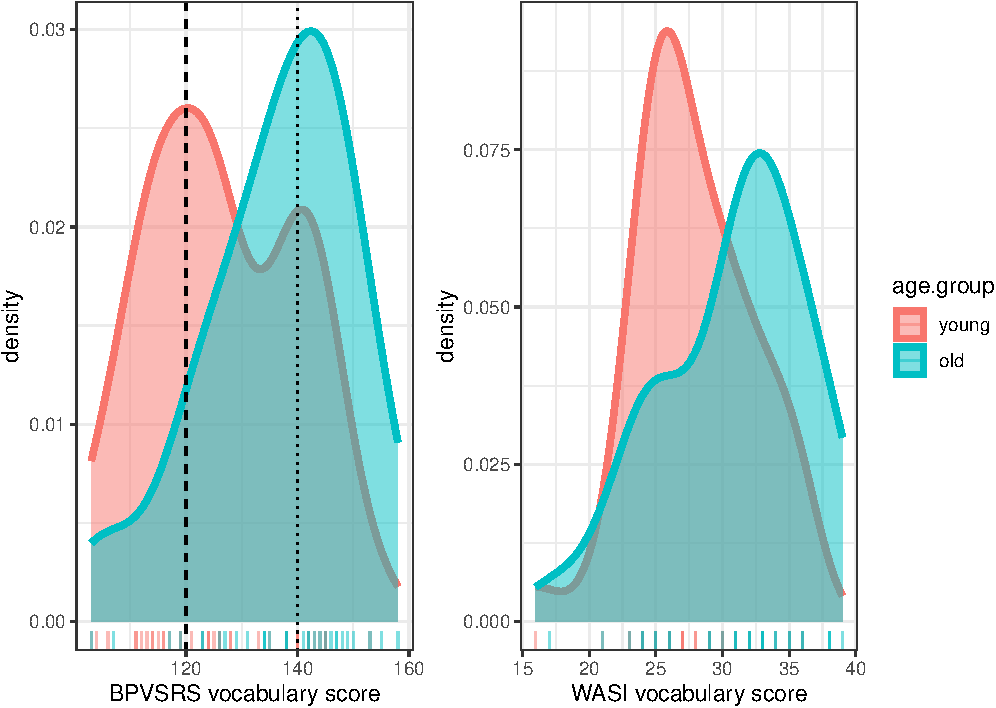
\includegraphics{visualization_files/figure-pdf/fig-density-BPVS-WASI-1.pdf}

}

\caption{\label{fig-density-BPVS-WASI}Distribution of childrens' scores
on the BPVS and WASI vocabulary measures.}

\end{figure}

Here is what the code does:

\begin{enumerate}
\def\labelenumi{\arabic{enumi}.}
\tightlist
\item
  \texttt{p.BPVRS.density\ \textless{}-\ ggplot(...)} creates a plot
  object called \texttt{p.BPVRS.density}.
\item
  \texttt{data\ =\ conc.orth.subjs,\ ...} says we use the
  \texttt{conc.orth.subjs} dataset to do this.
\item
  \texttt{aes(x\ =\ BPVRS,\ colour\ =\ age.group,\ fill\ =\ age.group))\ +}
  says we want to map \texttt{BPVRS} scores to x-axis location, and
  \texttt{age.group} level coding (\texttt{young,\ old}) to both
  \texttt{colour} and \texttt{fill}.
\item
  \texttt{geom\_density(alpha\ =\ .5,\ size\ =\ 1.5)\ +} draws a density
  plot; note that we said earlier what we want for \texttt{colour} and
  \texttt{fill} but here we also say that:
\end{enumerate}

\begin{itemize}
\tightlist
\item
  \texttt{alpha\ =\ .5} we want the fill to be transparent;
\item
  \texttt{size\ =\ 1.5} we want the density curve line to be thicker
  than usual.
\end{itemize}

\begin{enumerate}
\def\labelenumi{\arabic{enumi}.}
\setcounter{enumi}{4}
\tightlist
\item
  \texttt{geom\_rug(alpha\ =\ .5)\ +} adds a one-dimensional plot, a
  series of tick marks, to show where we have observations of
  \texttt{BPVRS} scores for specific children. We ask R to make the tick
  marks semi-transparent.
\item
  \texttt{geom\_vline(xintercept\ =\ 120,\ linetype\ =\ "dashed")\ +}
  draws a vertical dashed line where \texttt{BPVRS\ =\ 120}.
\item
  \texttt{geom\_vline(xintercept\ =\ 140,\ linetype\ =\ "dotted")\ +}
  draws a vertical dotted line where \texttt{BPVRS\ =\ 140}.
\item
  \texttt{labs(x\ =\ "BPVS\ vocabulary\ score")\ +} makes the x-axis
  label something understandable to someone who does not know about the
  study.
\item
  \texttt{theme\_bw()} changes the theme.
\end{enumerate}

\hypertarget{sec-group-compare-conclusions}{%
\paragraph{Critical evaluation: discovery and
communication}\label{sec-group-compare-conclusions}}

As we work with visualization, we should aim to develop skills in
reading plots, so:

\begin{itemize}
\tightlist
\item
  What do we see?
\end{itemize}

When we look at Figure~\ref{fig-density-BPVS-WASI}, we can see that the
younger and older children in the Ricketts et al. (2021) sample have
broadly overlapping distributions of vocabulary scores. However, as we
have noticed previously, the peak of the distribution is a bit lower for
the younger children compared to the older children. This appears to be
the case whether we are looking at the BPVS or at the WASI measures of
vocabulary, suggesting that the observation does not depend on the
particular vocabulary test. Is this observation unexpected? Probably
not, as we should hope to see vocabulary knowledge increase as children
get older. Is this observation a problem for our analysis? You need to
read the paper to find out what we decided.

\hypertarget{exercise-2}{%
\paragraph{Exercise}\label{exercise-2}}

In the demonstration examples, I focused on comparing age groups on
vocabulary, what about the other measures?

I used superimposed density plots: are other plotting styles more
effective, for you? Try using boxplots or superimposed or faceted
histograms instead.

\hypertarget{sec-summary-distributions}{%
\subsection{Summary: Visualizing
distributions}\label{sec-summary-distributions}}

So far, we have looked at how and why we may examine the distributions
of numeric variables. We have used histograms to visualize the
distribution of variable values. We have explored the construction of
grids of plots to enable the quick examination or concise communication
of information about the distributions of multiple variables at the same
time. And we have used histograms, boxplots and density plots to examine
how the distributions of variables may differ between groups.

The comparison of the distributions of variable values in different
groups (or, similarly, between different conditions) may be the kind of
work we would need to do, in data visualization, as part of an analysis
ending in, for example, a t-test comparison of mean values.

While boxplots, density plots and histograms are typically used to
examine how the values of a numeric variable vary, scatterplots are
typically used when we wish to examine, to make sense of or communicate
potential associations or relations between two (or more) numeric
variables. We turn to scatterplots, next.

\hypertarget{sec-examine-associations}{%
\subsection{Examine the associations between numeric
variables}\label{sec-examine-associations}}

Many of us start learning about scatterplots in high school math
classes. Using the modern tools made available to us through the
\texttt{ggplot2} library (as part of \texttt{tidyverse}), we can produce
effective, nice-looking, scatterplots for a range of discovery or
communication scenarios.

We continue working with the Ricketts et al. (2021) dataset. In the
context of the Ricketts et al. (2021) investigation, there is interest
in how children vary in the reading, spelling and vocabulary abilities
that may influence the capacity of children to learn new words. So, in
this context, we can begin to progress our development in visualization
skills by usefully considering the potential association between
participant attributes in the Study 2 sample.

Later on, we will look at more advanced plots that help us to
communicate the impact of the experimental manipulations implemented by
Ricketts et al. (2021), and also to discover the ways that these impacts
may vary between children.

\hypertarget{sec-scatter-basics}{%
\subsubsection{Getting started: Scatterplot
basics}\label{sec-scatter-basics}}

We can begin by asking a simple research question we can guess the
answer to:

\begin{itemize}
\tightlist
\item
  Do vocabulary knowledge scores on two alternative measures, the BPVS
  and the WASI, relate to each other?
\end{itemize}

If two measurement instruments or tests are intended to measure
individual differences in the same psychological attribute, here,
vocabulary knowledge, then we would reasonably expect that scores on one
test should covary with scores on the second test.

\begin{Shaded}
\begin{Highlighting}[numbers=left,,]
\FunctionTok{ggplot}\NormalTok{(}\AttributeTok{data =}\NormalTok{ conc.orth.subjs, }\FunctionTok{aes}\NormalTok{(}\AttributeTok{x =}\NormalTok{ WASIvRS, }\AttributeTok{y =}\NormalTok{ BPVSRS)) }\SpecialCharTok{+}
  \FunctionTok{geom\_point}\NormalTok{() }\SpecialCharTok{+}
  \FunctionTok{labs}\NormalTok{(}\AttributeTok{x =} \StringTok{"WASI vocabulary score"}\NormalTok{, }
       \AttributeTok{y =} \StringTok{"BPVSRS vocabulary score"}\NormalTok{,}
       \AttributeTok{title =} \StringTok{"Are WASI and BPVS vocabulary scores associated?"}\NormalTok{) }\SpecialCharTok{+}
  \FunctionTok{theme\_bw}\NormalTok{()}
\end{Highlighting}
\end{Shaded}

\begin{figure}[H]

{\centering 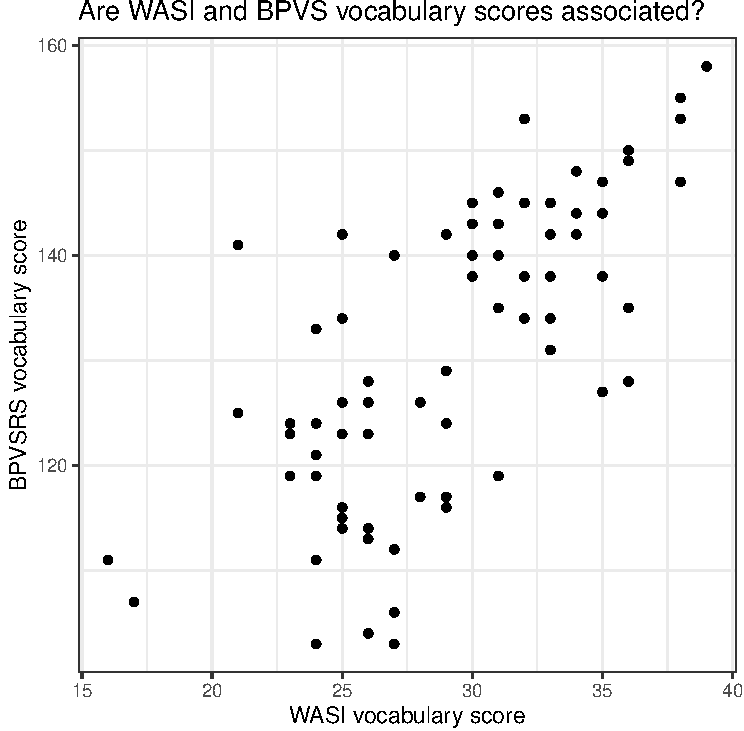
\includegraphics{visualization_files/figure-pdf/fig-scatter-BPVS-WASI-1.pdf}

}

\caption{\label{fig-scatter-BPVS-WASI}Scatterplot indicating the
potential association of childrens' scores on the BPVS and WASI
vocabulary measures.}

\end{figure}

What does the plot show us?

As a reminder of how scatterplots work, we can recall that they present
integrated information. Each point, for the Ricketts et al. (2021) data,
represents information about \emph{both} the BPVS \emph{and} the WASI
score for each child.

\begin{itemize}
\tightlist
\item
  The vertical height of a point tells us the BPVS score recorded for a
  child: higher points represent higher scores.
\item
  The left-to-right horizontal position of the same point tells us the
  WASI score for the same child: points located more on the right
  represent higher scores.
\end{itemize}

Figure~\ref{fig-scatter-BPVS-WASI} is a scatterplot comparing variation
in childrens' scores on the BPVS and WASI vocabulary measures: variation
in BPVS scores are shown on the y-axis and variation in WASI scores are
shown on the x-axis. Critically, the scientific insight the plot gives
us is this: higher WASI scores are associated with higher BPVS scores.

How does the code work? We have seen scatterplots before but, to ensure
we are comfortable with the coding, we can go through them step by step.

\begin{enumerate}
\def\labelenumi{\arabic{enumi}.}
\tightlist
\item
  \texttt{ggplot(data\ =\ conc.orth.subjs...)\ +} tells R we want to
  produce a plot using \texttt{ggplot()} with the
  \texttt{conc.orth.subjs} dataset.
\item
  \texttt{aes(x\ =\ WASIvRS,\ y\ =\ BPVSRS)} tells R that, in the plot,
  WASIvRS values are mapped to x-axis (horizontal) position and BPVSRS
  values are mapped to y-axis (vertical) position.
\item
  \texttt{geom\_point()\ +} constructs a scatterplot, using these data
  and these position mappings.
\item
  \texttt{labs(x\ =\ "WASI\ vocabulary\ score",\ ...} fixes the x-axis
  label.
\item
  \texttt{y\ =\ "BPVSRS\ vocabulary\ score",...} fixes the y-axis label.
\item
  \texttt{title\ =\ "Are\ WASI\ and\ BPVS\ vocabulary\ scores\ associated?")\ +}
  fixes the title.
\item
  \texttt{theme\_bw()} changes the theme.
\end{enumerate}

\hypertarget{sec-scatter-building}{%
\subsubsection{Building complexity: adding information step by
step}\label{sec-scatter-building}}

For this pair of variables in this dataset, the potential association in
the variation of scores is quite obvious. However, sometimes it is
helpful to guide the audience by imposing a \emph{smoother}. There are
different ways to do this, for different objectives and in different
contexts. Here, we look at two different approaches. In addition, as we
go, we examine how to adjust the appearance of the plot to address
different potential discovery or communication needs.

We begin by adding what is called a LOESS smoother.

\begin{Shaded}
\begin{Highlighting}[numbers=left,,]
\FunctionTok{ggplot}\NormalTok{(}\AttributeTok{data =}\NormalTok{ conc.orth.subjs, }\FunctionTok{aes}\NormalTok{(}\AttributeTok{x =}\NormalTok{ WASIvRS, }\AttributeTok{y =}\NormalTok{ BPVSRS)) }\SpecialCharTok{+}
  \FunctionTok{geom\_point}\NormalTok{() }\SpecialCharTok{+}
  \FunctionTok{geom\_smooth}\NormalTok{() }\SpecialCharTok{+}
  \FunctionTok{labs}\NormalTok{(}\AttributeTok{x =} \StringTok{"WASI vocabulary score"}\NormalTok{, }
       \AttributeTok{y =} \StringTok{"BPVSRS vocabulary score"}\NormalTok{,}
       \AttributeTok{title =} \StringTok{"Are WASI and BPVS vocabulary scores associated?"}\NormalTok{) }\SpecialCharTok{+}
  \FunctionTok{theme\_bw}\NormalTok{()}
\end{Highlighting}
\end{Shaded}

\begin{figure}[H]

{\centering 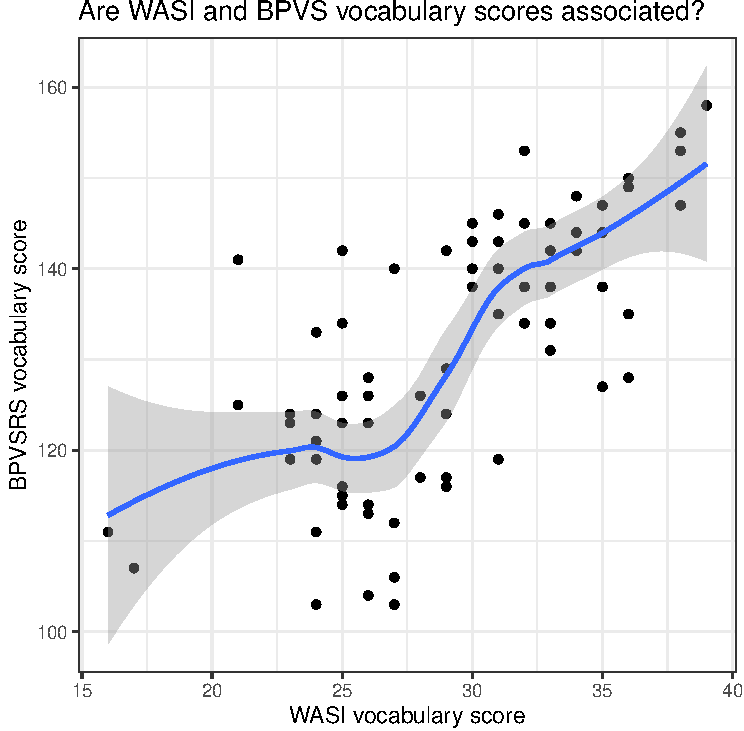
\includegraphics{visualization_files/figure-pdf/fig-scatter-BPVS-WASI-loess-1.pdf}

}

\caption{\label{fig-scatter-BPVS-WASI-loess}Scatterplot indicating the
potential association of childrens' scores on the BPVS and WASI
vocabulary measures.}

\end{figure}

The only coding difference between this plot
Figure~\ref{fig-scatter-BPVS-WASI-loess} and the previous plot
Figure~\ref{fig-scatter-BPVS-WASI} appears at line 3:

\begin{itemize}
\tightlist
\item
  \texttt{geom\_smooth()}
\end{itemize}

The addition of this bit of code results in the addition of the curving
line you see in Figure~\ref{fig-scatter-BPVS-WASI-loess}. The blue line
is curving, and visually suggests that the relation between BPVS and
WASI scores is different -- sometimes more sometimes less steep -- for
different values of WASI vocabulary score.

This line is generated by the \texttt{geom\_smooth()} code, by default,
in an approach in which the dataset is effectively split into sub-sets,
dividing the data up into sub-sets from the lowest to the highest WASI
scores, and the predicted association between the y-axis variable (here,
BPVS score) and the x-axis variable (here, WASI score) is calculated bit
by bit, in a series of regression analyses, working in order through
sub-sets of the data. This calculation of what is called the LOESS
(locally estimated scatterplot smoothing) trend is done by
\texttt{ggplot} for us. And this approach to visualizing the trend in a
potential association between variables is often a helpful way to
discover curved or non-linear relations.

You can find technical information on \texttt{geom\_smooth()}
\href{https://ggplot2.tidyverse.org/reference/geom_smooth.html}{here}
and an explanation of LOESS
\href{https://en.wikipedia.org/wiki/Local_regression}{here}.

For us, this default visualization is not helpful for two reasons:

\begin{enumerate}
\def\labelenumi{\arabic{enumi}.}
\tightlist
\item
  We have not yet learned about linear models, so learning about LOESS
  comes a bit early in our development.
\item
  It is hard to look at Figure~\ref{fig-scatter-BPVS-WASI-loess} and
  identify a convincing curvilinear relation between the two variables.
  A lot of the curve for low WASI scores appears to be linked to the
  presence of a small number of data points.
\end{enumerate}

At this stage, it is more helpful to adjust the addition of the
smoother. We can do that by adding an argument to the
\texttt{geom\_smooth()} function code.

\begin{Shaded}
\begin{Highlighting}[numbers=left,,]
\FunctionTok{ggplot}\NormalTok{(}\AttributeTok{data =}\NormalTok{ conc.orth.subjs, }\FunctionTok{aes}\NormalTok{(}\AttributeTok{x =}\NormalTok{ WASIvRS, }\AttributeTok{y =}\NormalTok{ BPVSRS)) }\SpecialCharTok{+}
  \FunctionTok{geom\_point}\NormalTok{() }\SpecialCharTok{+}
  \FunctionTok{geom\_smooth}\NormalTok{(}\AttributeTok{method =} \StringTok{\textquotesingle{}lm\textquotesingle{}}\NormalTok{) }\SpecialCharTok{+}
  \FunctionTok{labs}\NormalTok{(}\AttributeTok{x =} \StringTok{"WASI vocabulary score"}\NormalTok{, }
       \AttributeTok{y =} \StringTok{"BPVSRS vocabulary score"}\NormalTok{,}
       \AttributeTok{title =} \StringTok{"Are WASI and BPVS vocabulary scores associated?"}\NormalTok{) }\SpecialCharTok{+}
  \FunctionTok{theme\_bw}\NormalTok{()}
\end{Highlighting}
\end{Shaded}

\begin{figure}[H]

{\centering 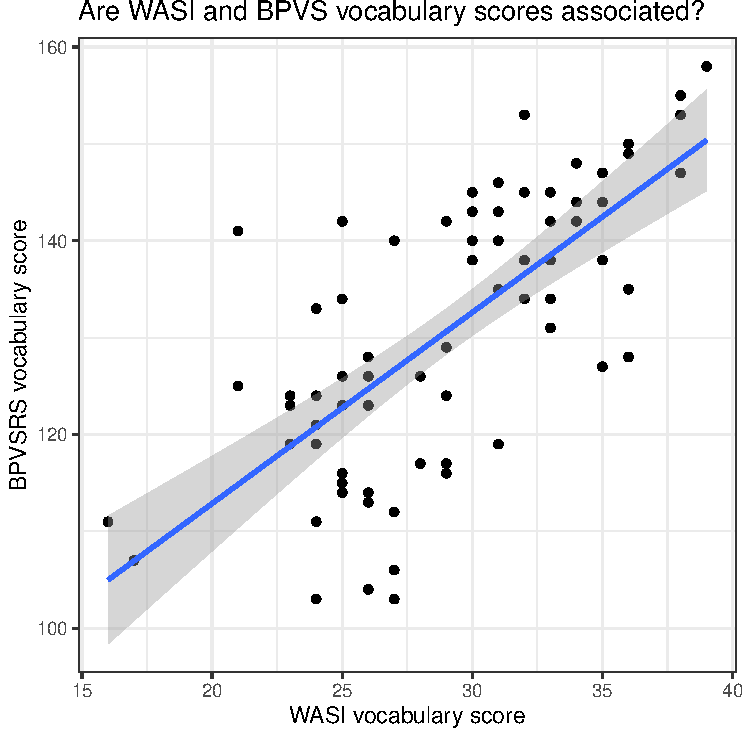
\includegraphics{visualization_files/figure-pdf/fig-scatter-BPVS-WASI-lm-1.pdf}

}

\caption{\label{fig-scatter-BPVS-WASI-lm}Scatterplot indicating the
potential association of childrens' scores on the BPVS and WASI
vocabulary measures.}

\end{figure}

Notice the difference between Figure~\ref{fig-scatter-BPVS-WASI-loess}
and Figure~\ref{fig-scatter-BPVS-WASI-lm}:

\begin{itemize}
\tightlist
\item
  \texttt{geom\_smooth(method\ =\ \textquotesingle{}lm\textquotesingle{})}
  tells R to draw a trend line, a smoother, using the \texttt{lm}
  method.
\end{itemize}

The \texttt{lm} method requires R to estimate the association between
the two variables, here, BPVS and WASI, assuming a linear model. Of
course, we are going to learn about linear models but, in short, right
now, what we need to know is that we assume a ``straight line''
relationship between the variables. This assumption requires that for
any interval of WASI scores -- e.g., whether we are talking about WASI
scores between 20-25 or about WASI scores between 30-35 -- the relation
between BPVS and WASI scores has the same shape: the direction and
steepness of the slope of the line is the same.

\hypertarget{exercise-3}{%
\subsubsection{Exercise}\label{exercise-3}}

Developing skill in working with data visualizations is not just about
developing coding skills, it is also about developing skills in reading,
and critically evaluating, the information the plots we produce show us.

Stop and take a good look at the scatterplot in
Figure~\ref{fig-scatter-BPVS-WASI-lm}. Use the visual representation of
data to critically evaluate the potential association between the BPVS
and WASI variables. What can you see?

You can train your critical evaluation by asking yourself questions like
the following:

\begin{enumerate}
\def\labelenumi{\arabic{enumi}.}
\tightlist
\item
  How does variation in the x-axis variable relate to variation in
  values of the y-axis variable?
\end{enumerate}

\begin{itemize}
\tightlist
\item
  We can see, here, that higher WASI scores are associated with higher
  BPVS scores.
\end{itemize}

\begin{enumerate}
\def\labelenumi{\arabic{enumi}.}
\setcounter{enumi}{1}
\tightlist
\item
  How strong is the relation?
\end{enumerate}

\begin{itemize}
\tightlist
\item
  The strength of the relation can be indicated by the steepness of the
  trend indicated by the smoother, here, the blue line.
\item
  If you track the position of the line, you can see, for example, that
  going from a WASI score of 20 to a WASI score of 40 is associated with
  going from a BPVS score of a little over 110 to a BPVS score of about
  a 150.
\item
  That seems like a big difference.
\end{itemize}

\begin{enumerate}
\def\labelenumi{\arabic{enumi}.}
\setcounter{enumi}{2}
\tightlist
\item
  How well does the trend we are looking at capture the data in our
  sample?
\end{enumerate}

\begin{itemize}
\tightlist
\item
  Here, we are concerned with how close the points are to the trend
  line.
\item
  If the trend line represents a set of predictions about how the BPVS
  scores vary (in height) given variation in WASI scores, we can see
  that in places the prediction is not very good.
\item
  Take a look at the points located at WASI 25. We can see that there
  there are points indicating that different children have the same WASI
  score of 25 but BPVS scores ranging from about 115 to 140.
\end{itemize}

\hypertarget{polish-the-appearance-of-a-plot-for-presentation}{%
\subsubsection{Polish the appearance of a plot for
presentation}\label{polish-the-appearance-of-a-plot-for-presentation}}

Figure~\ref{fig-scatter-BPVS-WASI-lm} presents a satisfactory looking
plot but it is worth checking what edits we can make to the appearance
of the plot, to indicate some of the ways that you can exercise choice
in determining what a plot looks like. This will be helpful to you when
you are constructing plots for presentation and report and you want to
ensure the plots are as effective as possible.

\begin{Shaded}
\begin{Highlighting}[numbers=left,,]
\FunctionTok{ggplot}\NormalTok{(}\AttributeTok{data =}\NormalTok{ conc.orth.subjs, }\FunctionTok{aes}\NormalTok{(}\AttributeTok{x =}\NormalTok{ WASIvRS, }\AttributeTok{y =}\NormalTok{ BPVSRS)) }\SpecialCharTok{+}
  \FunctionTok{geom\_point}\NormalTok{(}\AttributeTok{alpha =}\NormalTok{ .}\DecValTok{5}\NormalTok{, }\AttributeTok{size =} \DecValTok{2}\NormalTok{) }\SpecialCharTok{+}
  \FunctionTok{geom\_smooth}\NormalTok{(}\AttributeTok{method =} \StringTok{\textquotesingle{}lm\textquotesingle{}}\NormalTok{, }\AttributeTok{colour =} \StringTok{"red"}\NormalTok{, }\AttributeTok{size =} \FloatTok{1.5}\NormalTok{) }\SpecialCharTok{+}
  \FunctionTok{labs}\NormalTok{(}\AttributeTok{x =} \StringTok{"WASI vocabulary score"}\NormalTok{, }
       \AttributeTok{y =} \StringTok{"BPVSRS vocabulary score"}\NormalTok{,}
       \AttributeTok{title =} \StringTok{"Are WASI and BPVS vocabulary scores associated?"}\NormalTok{) }\SpecialCharTok{+}
  \FunctionTok{xlim}\NormalTok{(}\DecValTok{0}\NormalTok{, }\DecValTok{40}\NormalTok{) }\SpecialCharTok{+} \FunctionTok{ylim}\NormalTok{(}\DecValTok{0}\NormalTok{, }\DecValTok{160}\NormalTok{) }\SpecialCharTok{+}
  \FunctionTok{theme\_bw}\NormalTok{()}
\end{Highlighting}
\end{Shaded}

\begin{figure}[H]

{\centering 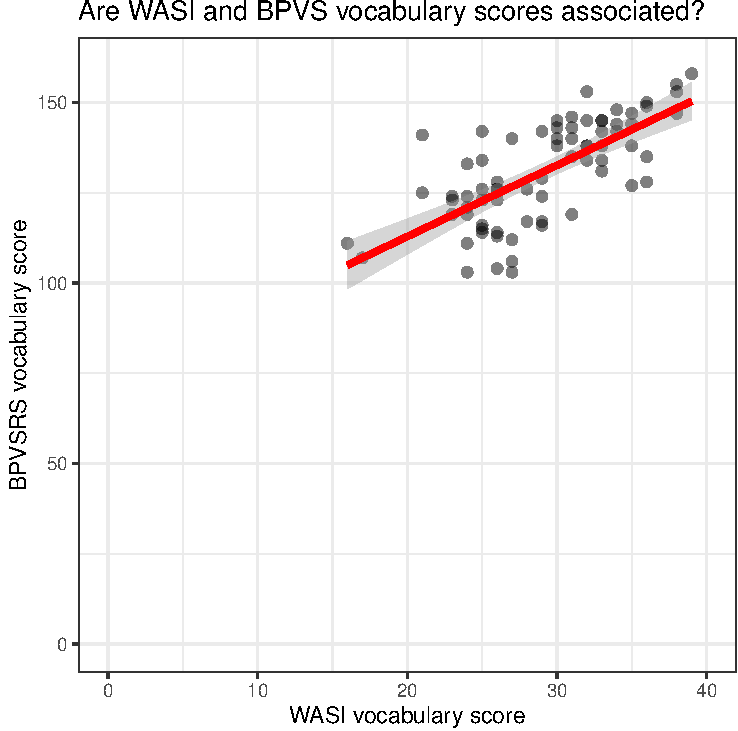
\includegraphics{visualization_files/figure-pdf/fig-scatter-BPVS-WASI-lm-edits-1.pdf}

}

\caption{\label{fig-scatter-BPVS-WASI-lm-edits}Scatterplot indicating
the potential association of childrens' scores on the BPVS and WASI
vocabulary measures.}

\end{figure}

If you inspect the code, you can see that I have made three changes:

\begin{enumerate}
\def\labelenumi{\arabic{enumi}.}
\tightlist
\item
  \texttt{geom\_point(alpha\ =\ .5,\ size\ =\ 2} changes the
  \texttt{size} of the points and their transparency (using
  \texttt{alpha}).
\item
  \texttt{geom\_smooth(method\ =\ \textquotesingle{}lm\textquotesingle{},\ colour\ =\ "red",\ size\ =\ 1.5)}
  change the \texttt{colour} of the smoother line, and the thickness
  (\texttt{size}) of the line.
\item
  \texttt{xlim(0,\ 40)\ +\ ylim(0,\ 160)} changes the axis limits.
\end{enumerate}

The last step --- changing the axis limits --- reveals how the sample
data can be understood in the context of possible scores on these
ability measures. Children \emph{could} get BPVS scores of 0 or WASI
scores of 0. By showing the start of the axes we get a more realistic
sense of how our sample compares to the possible ranges of scores we
could see in the wider population of children. This perhaps offers a
more honest or realistic visualization of the potential association
between BPVS and WASI vocabulary scores.

\hypertarget{sec-scatter-analysis-multiple}{%
\subsubsection{Examining associations among multiple
variables}\label{sec-scatter-analysis-multiple}}

As we have seen previously, we can construct a series of plots and
present them all at once in a grid or lattice.
Figure~\ref{fig-distribution-scatter-grid} presents just such a grid: of
scatterplots, indicating a series of potential associations.

Let's suppose that we are primarily interested in what factors influence
the extent to which children in the Ricketts et al. (2021) word learning
experiment are able to correctly spell the target words they were given
to learn. As explained earlier, in Section~\ref{sec-ricketts-study},
Ricketts et al. (2021) examined the spellings produced by participant
children in response to target words, counting how many string edits
(i.e., letter deletions etc.) separated the spelling each child produced
from the target spelling they should have produced.

We can calculate the mean spelling accuracy score for each child, over
all the target words we observed their response to. We can identify mean
spelling score as the \emph{outcome variable}. We can then examine
whether the outcome spelling scores are or are not influenced by
participant attributes like vocabulary knowledge.

Figure~\ref{fig-distribution-scatter-grid} presents a grid of
scatterplots indicating the potential association between mean spelling
score and each of the variables we have in the \texttt{conc.orth}
dataset, including the Castles and Coltheart (CC) and TOWRE measures of
word or nonword reading skill, WASI and BPVS measures of vocabulary
knowledge, and the WASI matrix measure of intelligence, as well as (our
newly coded) age group factor.

I hide an explanation of the coding behind the \texttt{Notes} tab,
because we have seen how to produce grids of plots, but you can take a
look if you want to learn how the plot is produced.

\section{Plot}

\begin{figure}

{\centering 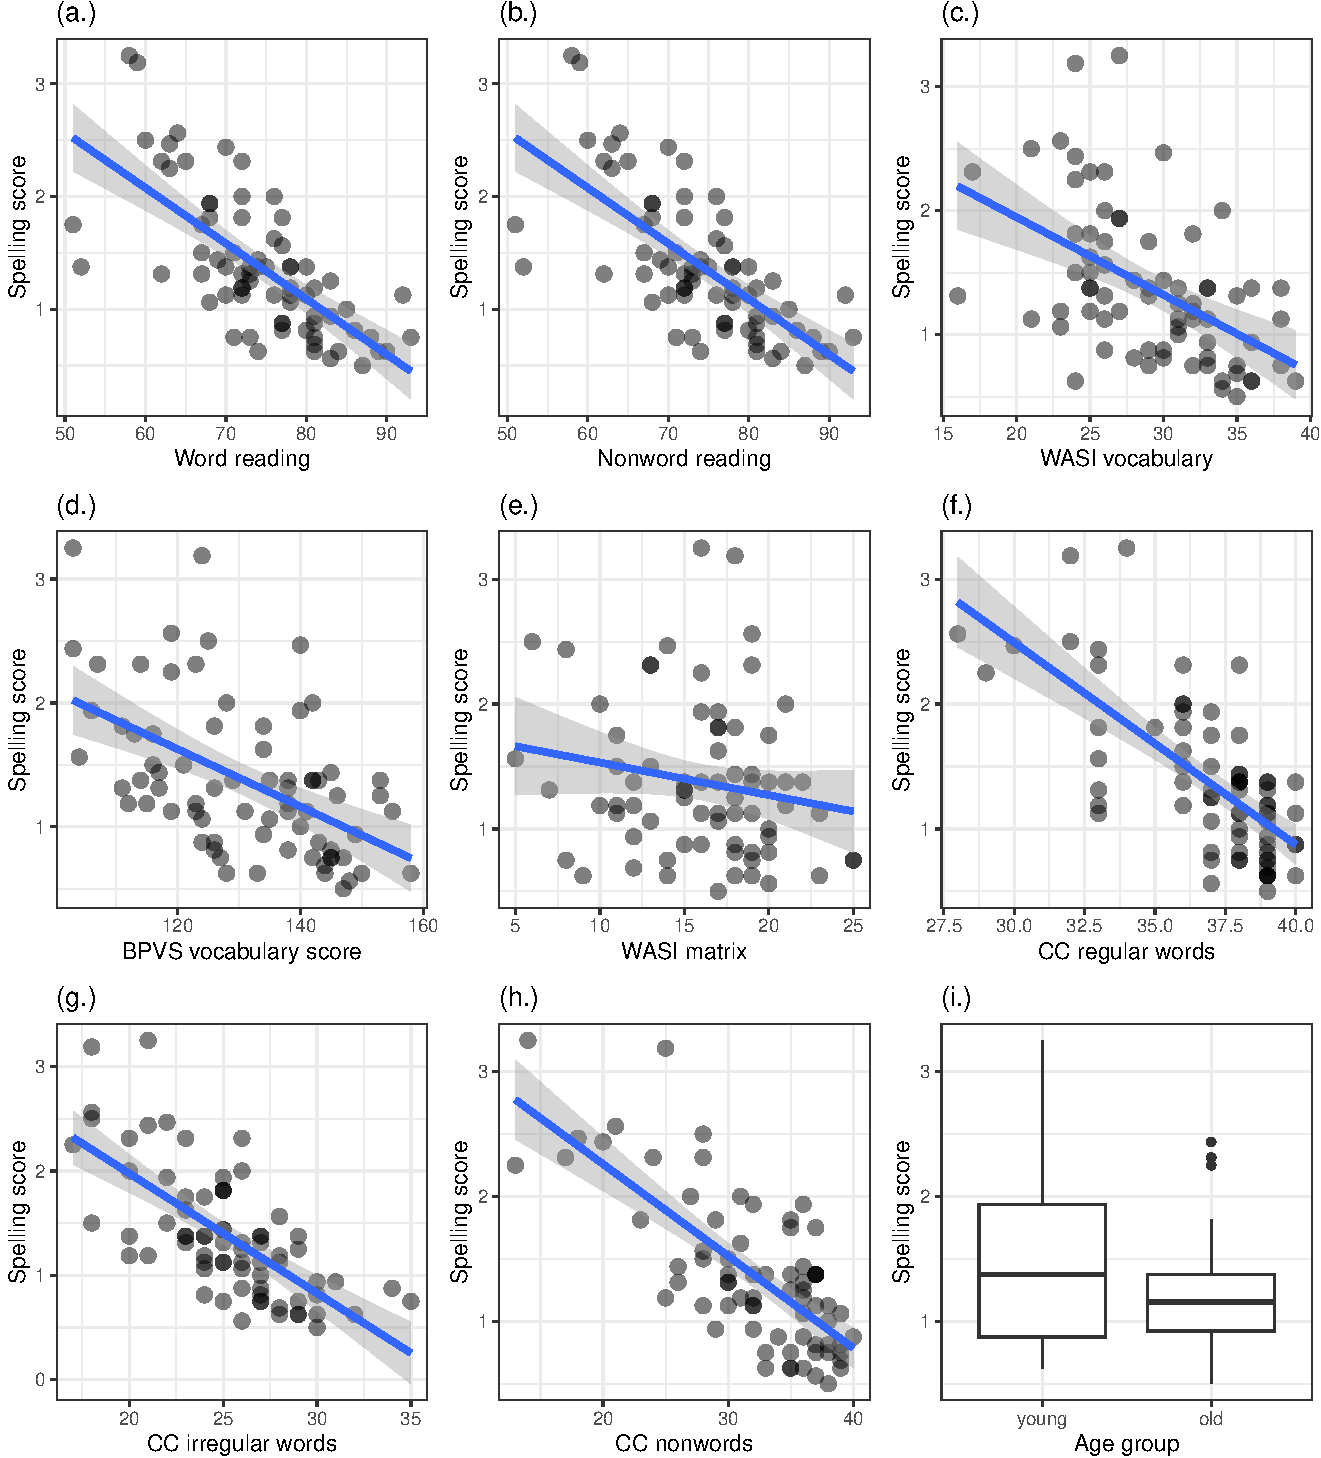
\includegraphics{visualization_files/figure-pdf/fig-distribution-scatter-grid-1.pdf}

}

\caption{\label{fig-distribution-scatter-grid}Grid of scatterplots
showing the potential association between mean spelling score, for each
child, and variation in the Castles and Coltheart (CC) and TOWRE
measures of word or nonword reading skill, WASI and BPVS measures of
vocabulary knowledge, the WASI matrix measure of intelligence, and age
group factor}

\end{figure}

\section{Notes}

The code to produce the figure is set out as follows.

\begin{Shaded}
\begin{Highlighting}[]
\NormalTok{p.wordsvsmean.score }\OtherTok{\textless{}{-}} \FunctionTok{ggplot}\NormalTok{(}\AttributeTok{data =}\NormalTok{ conc.orth.subjs, }
                              \FunctionTok{aes}\NormalTok{(}\AttributeTok{x =}\NormalTok{ TOWREsweRS, }
                              \AttributeTok{y =}\NormalTok{ mean.score)) }\SpecialCharTok{+}
  \FunctionTok{geom\_point}\NormalTok{(}\AttributeTok{alpha =}\NormalTok{ .}\DecValTok{5}\NormalTok{, }\AttributeTok{size =} \DecValTok{3}\NormalTok{) }\SpecialCharTok{+}
  \FunctionTok{geom\_smooth}\NormalTok{(}\AttributeTok{method =} \StringTok{\textquotesingle{}lm\textquotesingle{}}\NormalTok{, }\AttributeTok{size =} \FloatTok{1.5}\NormalTok{) }\SpecialCharTok{+}
  \FunctionTok{labs}\NormalTok{(}\AttributeTok{x =} \StringTok{"Word reading"}\NormalTok{, }
       \AttributeTok{y =} \StringTok{"Spelling score"}\NormalTok{,}
       \AttributeTok{title =} \StringTok{"(a.)"}\NormalTok{) }\SpecialCharTok{+}
  \FunctionTok{theme\_bw}\NormalTok{()}

\NormalTok{p.nonwordsvsmean.score }\OtherTok{\textless{}{-}} \FunctionTok{ggplot}\NormalTok{(}\AttributeTok{data =}\NormalTok{ conc.orth.subjs, }
                              \FunctionTok{aes}\NormalTok{(}\AttributeTok{x =}\NormalTok{ TOWREsweRS, }
                                  \AttributeTok{y =}\NormalTok{ mean.score)) }\SpecialCharTok{+}
  \FunctionTok{geom\_point}\NormalTok{(}\AttributeTok{alpha =}\NormalTok{ .}\DecValTok{5}\NormalTok{, }\AttributeTok{size =} \DecValTok{3}\NormalTok{) }\SpecialCharTok{+}
  \FunctionTok{geom\_smooth}\NormalTok{(}\AttributeTok{method =} \StringTok{\textquotesingle{}lm\textquotesingle{}}\NormalTok{, }\AttributeTok{size =} \FloatTok{1.5}\NormalTok{) }\SpecialCharTok{+}
  \FunctionTok{labs}\NormalTok{(}\AttributeTok{x =} \StringTok{"Nonword reading"}\NormalTok{, }
       \AttributeTok{y =} \StringTok{"Spelling score"}\NormalTok{,}
       \AttributeTok{title =} \StringTok{"(b.)"}\NormalTok{) }\SpecialCharTok{+}
  \FunctionTok{theme\_bw}\NormalTok{()}

\NormalTok{p.WASIvRSvsmean.score }\OtherTok{\textless{}{-}} \FunctionTok{ggplot}\NormalTok{(}\AttributeTok{data =}\NormalTok{ conc.orth.subjs, }
                              \FunctionTok{aes}\NormalTok{(}\AttributeTok{x =}\NormalTok{ WASIvRS, }
                                  \AttributeTok{y =}\NormalTok{ mean.score)) }\SpecialCharTok{+}
  \FunctionTok{geom\_point}\NormalTok{(}\AttributeTok{alpha =}\NormalTok{ .}\DecValTok{5}\NormalTok{, }\AttributeTok{size =} \DecValTok{3}\NormalTok{) }\SpecialCharTok{+}
  \FunctionTok{geom\_smooth}\NormalTok{(}\AttributeTok{method =} \StringTok{\textquotesingle{}lm\textquotesingle{}}\NormalTok{, }\AttributeTok{size =} \FloatTok{1.5}\NormalTok{) }\SpecialCharTok{+}
  \FunctionTok{labs}\NormalTok{(}\AttributeTok{x =} \StringTok{"WASI vocabulary"}\NormalTok{, }
       \AttributeTok{y =} \StringTok{"Spelling score"}\NormalTok{,}
       \AttributeTok{title =} \StringTok{"(c.)"}\NormalTok{) }\SpecialCharTok{+}
  \FunctionTok{theme\_bw}\NormalTok{()}

\NormalTok{p.BPVSRSvsmean.score }\OtherTok{\textless{}{-}} \FunctionTok{ggplot}\NormalTok{(}\AttributeTok{data =}\NormalTok{ conc.orth.subjs, }
                              \FunctionTok{aes}\NormalTok{(}\AttributeTok{x =}\NormalTok{ BPVSRS, }
                                  \AttributeTok{y =}\NormalTok{ mean.score)) }\SpecialCharTok{+}
  \FunctionTok{geom\_point}\NormalTok{(}\AttributeTok{alpha =}\NormalTok{ .}\DecValTok{5}\NormalTok{, }\AttributeTok{size =} \DecValTok{3}\NormalTok{) }\SpecialCharTok{+}
  \FunctionTok{geom\_smooth}\NormalTok{(}\AttributeTok{method =} \StringTok{\textquotesingle{}lm\textquotesingle{}}\NormalTok{, }\AttributeTok{size =} \FloatTok{1.5}\NormalTok{) }\SpecialCharTok{+}
  \FunctionTok{labs}\NormalTok{(}\AttributeTok{x =} \StringTok{"BPVS vocabulary score"}\NormalTok{, }
       \AttributeTok{y =} \StringTok{"Spelling score"}\NormalTok{,}
       \AttributeTok{title =} \StringTok{"(d.)"}\NormalTok{) }\SpecialCharTok{+}
  \FunctionTok{theme\_bw}\NormalTok{()}

\NormalTok{p.WASImRSvsmean.score }\OtherTok{\textless{}{-}} \FunctionTok{ggplot}\NormalTok{(}\AttributeTok{data =}\NormalTok{ conc.orth.subjs, }
                              \FunctionTok{aes}\NormalTok{(}\AttributeTok{x =}\NormalTok{ WASImRS, }
                                  \AttributeTok{y =}\NormalTok{ mean.score)) }\SpecialCharTok{+}
  \FunctionTok{geom\_point}\NormalTok{(}\AttributeTok{alpha =}\NormalTok{ .}\DecValTok{5}\NormalTok{, }\AttributeTok{size =} \DecValTok{3}\NormalTok{) }\SpecialCharTok{+}
  \FunctionTok{geom\_smooth}\NormalTok{(}\AttributeTok{method =} \StringTok{\textquotesingle{}lm\textquotesingle{}}\NormalTok{, }\AttributeTok{size =} \FloatTok{1.5}\NormalTok{) }\SpecialCharTok{+}
  \FunctionTok{labs}\NormalTok{(}\AttributeTok{x =} \StringTok{"WASI matrix"}\NormalTok{, }
       \AttributeTok{y =} \StringTok{"Spelling score"}\NormalTok{,}
       \AttributeTok{title =} \StringTok{"(e.)"}\NormalTok{) }\SpecialCharTok{+}
  \FunctionTok{theme\_bw}\NormalTok{()}

\NormalTok{p.CC2regRSvsmean.score }\OtherTok{\textless{}{-}} \FunctionTok{ggplot}\NormalTok{(}\AttributeTok{data =}\NormalTok{ conc.orth.subjs, }
                              \FunctionTok{aes}\NormalTok{(}\AttributeTok{x =}\NormalTok{ CC2regRS, }
                                  \AttributeTok{y =}\NormalTok{ mean.score)) }\SpecialCharTok{+}
  \FunctionTok{geom\_point}\NormalTok{(}\AttributeTok{alpha =}\NormalTok{ .}\DecValTok{5}\NormalTok{, }\AttributeTok{size =} \DecValTok{3}\NormalTok{) }\SpecialCharTok{+}
  \FunctionTok{geom\_smooth}\NormalTok{(}\AttributeTok{method =} \StringTok{\textquotesingle{}lm\textquotesingle{}}\NormalTok{, }\AttributeTok{size =} \FloatTok{1.5}\NormalTok{) }\SpecialCharTok{+}
  \FunctionTok{labs}\NormalTok{(}\AttributeTok{x =} \StringTok{"CC regular words"}\NormalTok{, }
       \AttributeTok{y =} \StringTok{"Spelling score"}\NormalTok{,}
       \AttributeTok{title =} \StringTok{"(f.)"}\NormalTok{) }\SpecialCharTok{+}
  \FunctionTok{theme\_bw}\NormalTok{()}

\NormalTok{p.CC2irregRSvsmean.score }\OtherTok{\textless{}{-}} \FunctionTok{ggplot}\NormalTok{(}\AttributeTok{data =}\NormalTok{ conc.orth.subjs, }
                              \FunctionTok{aes}\NormalTok{(}\AttributeTok{x =}\NormalTok{ CC2irregRS, }
                                  \AttributeTok{y =}\NormalTok{ mean.score)) }\SpecialCharTok{+}
  \FunctionTok{geom\_point}\NormalTok{(}\AttributeTok{alpha =}\NormalTok{ .}\DecValTok{5}\NormalTok{, }\AttributeTok{size =} \DecValTok{3}\NormalTok{) }\SpecialCharTok{+}
  \FunctionTok{geom\_smooth}\NormalTok{(}\AttributeTok{method =} \StringTok{\textquotesingle{}lm\textquotesingle{}}\NormalTok{, }\AttributeTok{size =} \FloatTok{1.5}\NormalTok{) }\SpecialCharTok{+}
  \FunctionTok{labs}\NormalTok{(}\AttributeTok{x =} \StringTok{"CC irregular words"}\NormalTok{, }
       \AttributeTok{y =} \StringTok{"Spelling score"}\NormalTok{,}
       \AttributeTok{title =} \StringTok{"(g.)"}\NormalTok{) }\SpecialCharTok{+}
  \FunctionTok{theme\_bw}\NormalTok{()}

\NormalTok{p.CC2nwRSvsmean.score }\OtherTok{\textless{}{-}} \FunctionTok{ggplot}\NormalTok{(}\AttributeTok{data =}\NormalTok{ conc.orth.subjs, }
                              \FunctionTok{aes}\NormalTok{(}\AttributeTok{x =}\NormalTok{ CC2nwRS, }
                                  \AttributeTok{y =}\NormalTok{ mean.score)) }\SpecialCharTok{+}
  \FunctionTok{geom\_point}\NormalTok{(}\AttributeTok{alpha =}\NormalTok{ .}\DecValTok{5}\NormalTok{, }\AttributeTok{size =} \DecValTok{3}\NormalTok{) }\SpecialCharTok{+}
  \FunctionTok{geom\_smooth}\NormalTok{(}\AttributeTok{method =} \StringTok{\textquotesingle{}lm\textquotesingle{}}\NormalTok{, }\AttributeTok{size =} \FloatTok{1.5}\NormalTok{) }\SpecialCharTok{+}
  \FunctionTok{labs}\NormalTok{(}\AttributeTok{x =} \StringTok{"CC nonwords"}\NormalTok{, }
       \AttributeTok{y =} \StringTok{"Spelling score"}\NormalTok{,}
       \AttributeTok{title =} \StringTok{"(h.)"}\NormalTok{) }\SpecialCharTok{+}
  \FunctionTok{theme\_bw}\NormalTok{()}

\NormalTok{p.age.groupvsmean.score }\OtherTok{\textless{}{-}} \FunctionTok{ggplot}\NormalTok{(}\AttributeTok{data =}\NormalTok{ conc.orth.subjs, }
                              \FunctionTok{aes}\NormalTok{(}\AttributeTok{x =}\NormalTok{ age.group, }
                                  \AttributeTok{y =}\NormalTok{ mean.score)) }\SpecialCharTok{+}
  \FunctionTok{geom\_boxplot}\NormalTok{() }\SpecialCharTok{+}
  \FunctionTok{labs}\NormalTok{(}\AttributeTok{x =} \StringTok{"Age group"}\NormalTok{, }
       \AttributeTok{y =} \StringTok{"Spelling score"}\NormalTok{,}
       \AttributeTok{title =} \StringTok{"(i.)"}\NormalTok{) }\SpecialCharTok{+}
  \FunctionTok{theme\_bw}\NormalTok{()}

\NormalTok{p.wordsvsmean.score }\SpecialCharTok{+}\NormalTok{ p.nonwordsvsmean.score }\SpecialCharTok{+}\NormalTok{ p.WASIvRSvsmean.score }\SpecialCharTok{+}
\NormalTok{  p.BPVSRSvsmean.score }\SpecialCharTok{+}\NormalTok{ p.WASImRSvsmean.score }\SpecialCharTok{+}\NormalTok{ p.CC2regRSvsmean.score }\SpecialCharTok{+}
\NormalTok{  p.CC2irregRSvsmean.score }\SpecialCharTok{+}\NormalTok{ p.CC2nwRSvsmean.score }\SpecialCharTok{+}\NormalTok{ p.age.groupvsmean.score}
\end{Highlighting}
\end{Shaded}

\begin{enumerate}
\def\labelenumi{\arabic{enumi}.}
\tightlist
\item
  To produce the grid of plots, we first create a series of plot objects
  using code like that shown in the chunk.
\end{enumerate}

\begin{Shaded}
\begin{Highlighting}[]
\NormalTok{p.wordsvsmean.score }\OtherTok{\textless{}{-}} \FunctionTok{ggplot}\NormalTok{(}\AttributeTok{data =}\NormalTok{ conc.orth.subjs, }
                              \FunctionTok{aes}\NormalTok{(}\AttributeTok{x =}\NormalTok{ TOWREsweRS, }
                              \AttributeTok{y =}\NormalTok{ mean.score)) }\SpecialCharTok{+}
  \FunctionTok{geom\_point}\NormalTok{(}\AttributeTok{alpha =}\NormalTok{ .}\DecValTok{5}\NormalTok{, }\AttributeTok{size =} \DecValTok{3}\NormalTok{) }\SpecialCharTok{+}
  \FunctionTok{geom\_smooth}\NormalTok{(}\AttributeTok{method =} \StringTok{\textquotesingle{}lm\textquotesingle{}}\NormalTok{, }\AttributeTok{size =} \FloatTok{1.5}\NormalTok{) }\SpecialCharTok{+}
  \FunctionTok{labs}\NormalTok{(}\AttributeTok{x =} \StringTok{"Word reading"}\NormalTok{, }
       \AttributeTok{y =} \StringTok{"Spelling score"}\NormalTok{,}
       \AttributeTok{title =} \StringTok{"(a.)"}\NormalTok{) }\SpecialCharTok{+}
  \FunctionTok{theme\_bw}\NormalTok{()}
\end{Highlighting}
\end{Shaded}

\begin{itemize}
\tightlist
\item
  \texttt{p.wordsvsmean.score\ \textless{}-\ ggplot(...)} creates the
  plot.
\item
  \texttt{data\ =\ conc.orth.subjs} tells R what data to work with.
\item
  \texttt{aes(x\ =\ TOWREsweRS,\ y\ =\ mean.score)} specifies the
  aesthetic data mappings.
\item
  \texttt{geom\_point(alpha\ =\ .5,\ size\ =\ 3)} tells R to produce a
  scatterplot, specifying the size and transparency of the points.
\item
  \texttt{geom\_smooth(method\ =\ \textquotesingle{}lm\textquotesingle{},\ size\ =\ 1.5)}
  tells R to add a smoother, specifying the method and the thickness of
  the line.
\item
  \texttt{labs(x\ =\ "Word\ reading",\ y\ =\ "Spelling\ score",\ title\ =\ "(a.)")}
  fixes the labels.
\item
  \texttt{theme\_bw()} adjusts the theme.
\end{itemize}

\begin{enumerate}
\def\labelenumi{\arabic{enumi}.}
\setcounter{enumi}{1}
\tightlist
\item
  We then put the plots together, using the \texttt{patchwork} syntax
  where we list the plot objects by name, separating each name by a
  \texttt{+}.
\end{enumerate}

\begin{Shaded}
\begin{Highlighting}[]
\NormalTok{p.BPVSRSvsmean.score }\SpecialCharTok{+}\NormalTok{ p.WASImRSvsmean.score }\SpecialCharTok{+}\NormalTok{ p.CC2regRSvsmean.score }\SpecialCharTok{+}
\NormalTok{  p.CC2irregRSvsmean.score }\SpecialCharTok{+}\NormalTok{ p.CC2nwRSvsmean.score }\SpecialCharTok{+}\NormalTok{ p.age.groupvsmean.score}
\end{Highlighting}
\end{Shaded}

Figure~\ref{fig-distribution-scatter-grid} allows us to visually
represent the potential association between an outcome measure, the
average spelling score, and a series of other variables that may or may
not have an influence on that outcome. Using a grid in this fashion
allows us to compare the extent to which different variables appear to
have an influence on the outcome. We can see, for example, that measures
of variation in word reading skill appear to have stronger association
(the trend lines are more steeply slowed) than measures of vocabulary
knowledge or intelligence, or age group.

Using grids of plots like this allow us to compactly communicate these
potential associations in a single figure.

\begin{tcolorbox}[enhanced jigsaw, opacitybacktitle=0.6, title=\textcolor{quarto-callout-warning-color}{\faExclamationTriangle}\hspace{0.5em}{Warning}, arc=.35mm, colbacktitle=quarto-callout-warning-color!10!white, colframe=quarto-callout-warning-color-frame, leftrule=.75mm, opacityback=0, breakable, titlerule=0mm, left=2mm, bottomrule=.15mm, toprule=.15mm, colback=white, coltitle=black, bottomtitle=1mm, toptitle=1mm, rightrule=.15mm]

Levenshtein distance scores are higher \emph{if} a child makes more
errors in producing the letters in a spelling response.

\begin{itemize}
\tightlist
\item
  This means that if we want to see what factors help a child to learn a
  word, including its spelling, then we want to see that helpful factors
  are associated with \emph{lower} Levenshtein scores.
\end{itemize}

\end{tcolorbox}

\hypertarget{sec-visualize-effects}{%
\subsection{Answering a scientific question: Visualize the effects of
experimental conditions}\label{sec-visualize-effects}}

As explained in Section~\ref{sec-ricketts-study}, in the Ricketts et al.
(2021) study, we taught children taught 16 novel words in a study with a
\emph{2 x 2} factorial design. The presence of orthography (orthography
absent vs.~orthography present) was manipulated within participants: for
all children, eight of the words were taught with orthography (the word
spelling) present and eight with orthography absent. Instructions
(incidental vs.~explicit) were manipulated between participants such
that children in the explicit condition were alerted to the presence of
orthography whereas children in the incidental condition were not. The
Ricketts et al. (2021) investigation was primarily concerned with the
effects on word learning of presenting words for learning with or
without showing the words with their spellings, with or without
instructing students explicitly that they would be helped by the
presence of the spellings.

We can analyze the effects of orthography and instruction using a linear
model.

\begin{Shaded}
\begin{Highlighting}[]
\NormalTok{model }\OtherTok{\textless{}{-}} \FunctionTok{lm}\NormalTok{(Levenshtein.Score }\SpecialCharTok{\textasciitilde{}}\NormalTok{ Instructions}\SpecialCharTok{*}\NormalTok{Orthography, }\AttributeTok{data =}\NormalTok{ conc.orth)}
\end{Highlighting}
\end{Shaded}

The model code estimates variation in spelling score (values of the
\texttt{Levenshtein.Score}) variable, given variation in the levels of
the \texttt{Instructions} and \texttt{Orthography} factors, and their
interaction.

This model is a \emph{limited} approximation of the analysis we would
need to do with these data to estimate the effects of orthography and
instruction; see Ricketts et al. (2021) for more information on what
analysis is required (in our view). However, it is good enough as a
basis for exploring the kind of data visualization work --- in terms of
both discovery and communication --- that you can do when you are
working with data from an experimental study.

We can get a summary of the model results which presents the estimated
effect of each experimental factor. These estimates represent the
predicted change in spelling score, given variation in Orthography
(present, absent) or Instruction (explicit, incidental), and given the
possibility that the effect of the presence of orthography is different
for different levels of instruction.

Notice that some of the p-values are incorrectly shown as
\texttt{0.000}. This is a result of using functions to automatically
take a model summary and generate a table. I am going to leave this
error with a warning because our focus is on visualization, next.

\begin{table}

\caption{Model summary}
\centering
\begin{tabular}[t]{l|r|r|r|r}
\hline
term & estimate & std.error & statistic & p.value\\
\hline
(Intercept) & 1.584 & 0.072 & 21.857 & 0.000\\
\hline
Instructionsincidental & -0.041 & 0.103 & -0.396 & 0.692\\
\hline
Orthographypresent & -0.409 & 0.103 & -3.987 & 0.000\\
\hline
Instructionsincidental:Orthographypresent & 0.060 & 0.146 & 0.409 & 0.683\\
\hline
\end{tabular}
\end{table}

Very often, when we complete a statistical analysis of outcome data, in
which we estimate or test the effects on outcomes of variation in some
variables or of variation in experimental conditions, then we present a
table summary of the analysis results. However, these estimates are
typically difficult to interpret (it gets easier with practice) and talk
about. Take a look at the summary table. We are often to focus on
whether effects are significant or not significant. But, really, what we
should consider is \emph{how much} the outcome changes given the
different experimental conditions.

How do we get that information from the analysis results? We can
communicate results --- to ourselves or to an audience --- by
constructing plots from the model information. The \texttt{ggeffects}
library extends \texttt{ggplot2} to enable us to do this quite
efficiently.

When we write code to fit a linear model like:

\begin{Shaded}
\begin{Highlighting}[]
\NormalTok{model }\OtherTok{\textless{}{-}} \FunctionTok{lm}\NormalTok{(Levenshtein.Score }\SpecialCharTok{\textasciitilde{}}\NormalTok{ Instructions}\SpecialCharTok{*}\NormalTok{Orthography, }\AttributeTok{data =}\NormalTok{ conc.orth)}
\end{Highlighting}
\end{Shaded}

We record the results as an object called \texttt{model} because we
specify \texttt{model\ \textless{}-\ lm(...)}. We can take these results
and ask R to create a plot showing predicted change in outcome
(spelling) given our model. We can then present the effects of the
variables, as shown in Figure~\ref{fig-effects-dotwhisker}.

\begin{Shaded}
\begin{Highlighting}[numbers=left,,]
\NormalTok{dat }\OtherTok{\textless{}{-}} \FunctionTok{ggpredict}\NormalTok{(model, }\AttributeTok{terms =} \FunctionTok{c}\NormalTok{(}\StringTok{"Instructions"}\NormalTok{, }\StringTok{"Orthography"}\NormalTok{))}
\FunctionTok{plot}\NormalTok{(dat, }\AttributeTok{facet =} \ConstantTok{TRUE}\NormalTok{) }\SpecialCharTok{+} \FunctionTok{ylim}\NormalTok{(}\DecValTok{0}\NormalTok{, }\DecValTok{3}\NormalTok{)}
\end{Highlighting}
\end{Shaded}

\begin{figure}[H]

{\centering 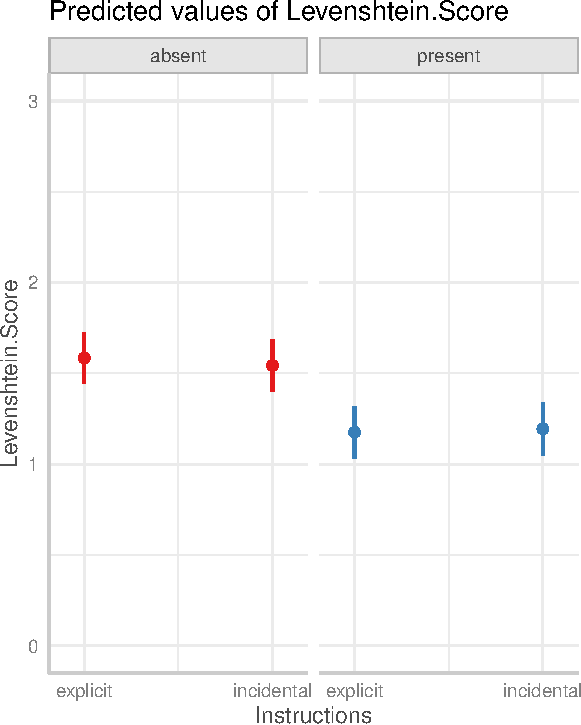
\includegraphics{visualization_files/figure-pdf/fig-effects-dotwhisker-1.pdf}

}

\caption{\label{fig-effects-dotwhisker}Dot and whisker plots showing the
predicted effect on outcome spelling (Levenshtein) score, given
different experimental conditions: Orthography (present, absent) x
Instruction (explicit, incidental).}

\end{figure}

The code works as follows:

\begin{enumerate}
\def\labelenumi{\arabic{enumi}.}
\tightlist
\item
  \texttt{dat\ \textless{}-\ ggpredict(model,\ terms\ =\ c("Instructions",\ "Orthography"))}
  tells R to calculate predicted outcomes, given our \texttt{model}
  information, for the factors \texttt{"Instructions",\ "Orthography"}.
\item
  \texttt{plot(dat,\ facet\ =\ TRUE)} plot the effects, given the
  predictions, showing the effect of different instruction conditions in
  different plot facets (the left and right panels).
\item
  \texttt{ylim(0,\ 3)} fix the y-axis to show a more honest indication
  of the effect on outcomes, given the potential range of spelling
  scores can start at 0.
\end{enumerate}

In Figure~\ref{fig-effects-dotwhisker}, the dots represent the linear
model estimates of outcome spelling, predicted under different
conditions. The plots indicate that spelling scores are predicted to be
lower when orthography is present. There appears to be little or no
effect associated with different kinds of instruction.

The vertical lines (often termed ``whiskers'') indicate the 95\%
confidence interval about these estimates. Confidence intervals (CIs)
are often mis-interpreted so I will give the quick definition outlined
by Hoekstra et al. (2014) here:

\begin{quote}
A CI is a numerical interval constructed around the estimate of a
parameter {[}i.e.~the model estimate of the effect{]}. Such an interval
does not, however, directly indicate a property of the parameter;
instead, it indicates a property of the procedure, as is typical for a
frequentist technique. Specifically, we may find that a particular
procedure, when used repeatedly across a series of hypothetical data
sets (i.e., the sample space), yields intervals that contain the true
parameter value in 95 \% of the cases.
\end{quote}

In short, the interval shows us the range of values within which we can
expect to capture the effects of interest, in the long run, if we were
to run our experiment over and over again.

Given our data and our model, these intervals indicate where the outcome
might be expected to vary, given different conditions, and that is quite
useful information. If you look at Figure~\ref{fig-effects-dotwhisker},
you can see that the presence of orthography (present versus absent)
appears to shift outcome spelling, on average, by about a quarter of a
letter edit: from over 1.5 to about 1.25. This is about one quarter of
the difference, on average, between getting a target spelling correct
and getting it wrong by one letter (e.g., the response `epegram' for the
target `epigram'). This is a relatively small effect but we may consider
how such small effects add up, over a child's development, cumulatively,
in making the difference between wrong or nearly right spellings to
correct spellings.

In the Ricketts et al. (2021) paper, we conducted \emph{Bayesian}
analyses which allow us to plot the estimated effects of experimental
conditions along with what are called \emph{credible} intervals
indicating our uncertainty about the estimates. In a Bayesian analysis,
we can indicate the probable or plausible effect of conditions, or range
of plausible effects, given our data and our model. (This intuitive
sense of the probable location of effects is, sometimes, what
researchers and students mis-interpret confidence intervals as showing;
Hoekstra et al. (2014).) Accounting for our uncertainty is a productive
approach to considering how much we learn from the evidence we collect
in experiments.

But this gets ahead of where we are now in our development of skills and
understanding. There is another way to discover how uncertain we may be
about the results of our analysis. This is an approach we have already
experienced: plotting trends or estimates together with the observed
data points. We present an example in
Figure~\ref{fig-effects-dotwhisker-raw}.

\begin{Shaded}
\begin{Highlighting}[numbers=left,,]
\FunctionTok{plot}\NormalTok{(dat, }\AttributeTok{add.data =} \ConstantTok{TRUE}\NormalTok{)}
\end{Highlighting}
\end{Shaded}

\begin{figure}[H]

{\centering 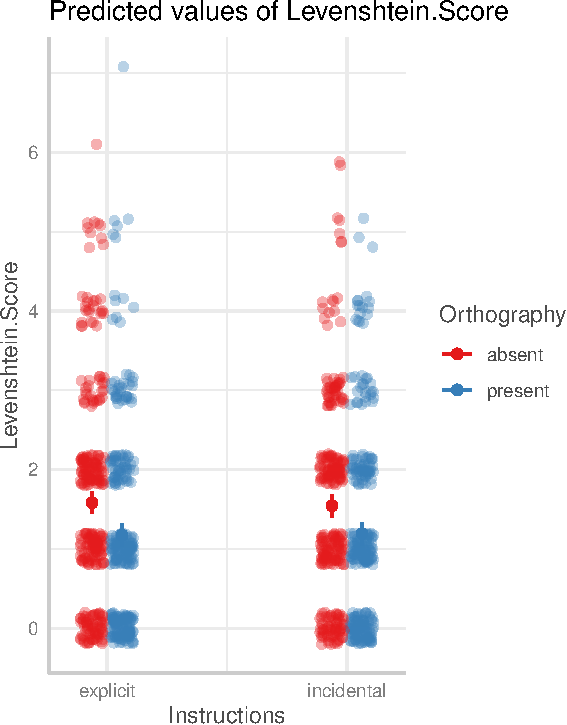
\includegraphics{visualization_files/figure-pdf/fig-effects-dotwhisker-raw-1.pdf}

}

\caption{\label{fig-effects-dotwhisker-raw}Dot and whisker plots showing
the predicted effect on outcome spelling (Levenshtein) score, given
different experimental conditions: Orthography (present, absent) x
Instruction (explicit, incidental). The estimates are shown as
dot-whisker points. In addition, the plot shows as points the spelling
score observed for each child for each response recorded in the
\texttt{conc.orth} dataset.}

\end{figure}

Figure~\ref{fig-effects-dotwhisker-raw} reveals the usefulness of
plotting model estimates of effects alongside the raw observed outcomes.
We can make two critical observations.

\begin{enumerate}
\def\labelenumi{\arabic{enumi}.}
\tightlist
\item
  We can see that the observed scores clearly cluster around outcome
  spelling values of 0, 1, 2, 3, 4, and 5.
\end{enumerate}

\begin{itemize}
\tightlist
\item
  This is not a surprise because Ricketts et al. (2021) scored each
  response in their test of spelling knowledge by counting the number of
  letter edits (letter deletions, additions etc.) separating a spelling
  response from a target response.
\item
  But the plot does suggest that the linear model is missing something
  about the outcome data because there is no recognition in the model or
  the results of this bunching or clustering around whole number values
  of the outcome variable. (This is why Ricketts et al. (2021) use a
  different analysis approach.)
\end{itemize}

\begin{enumerate}
\def\labelenumi{\arabic{enumi}.}
\setcounter{enumi}{1}
\tightlist
\item
  We can also see that it is actually quite difficult to distinguish the
  effects of the experimental condition differences on the observed
  spelling responses. There is a lot of variation in the responses.
\end{enumerate}

How can we make sense of this variation?

Another approach we can take to experimental data is to examine visually
how the effects of experimental conditions vary between individual
participants. Usually, in teaching, learning and doing foundation or
introductory statistical analyses we think about the \emph{average
impact} on outcomes of the experimental conditions or some set of
predictor variables. It often makes sense, also, or instead, to consider
the ways that the impact on outcomes vary between individuals.

Here, it might be worthwhile to look at the effect of the conditions for
each child. We can do that in different ways. In the following, we will
look at a couple of approaches that are often useful. We will focus on
the effect of variation in the Orthography condition (present, absent)

To begin our work, we first calculate the average outcome
(\texttt{Levenshtein.Score}) spelling score for each child in each of
the experimental conditions (\texttt{Orthography}, present versus
absent):

We do this in a series of steps.

\begin{Shaded}
\begin{Highlighting}[numbers=left,,]
\NormalTok{score.by.subj }\OtherTok{\textless{}{-}}\NormalTok{ conc.orth }\SpecialCharTok{\%\textgreater{}\%}
  \FunctionTok{group\_by}\NormalTok{(Participant, Orthography) }\SpecialCharTok{\%\textgreater{}\%}
  \FunctionTok{summarise}\NormalTok{(}\AttributeTok{mean.score =} \FunctionTok{mean}\NormalTok{(Levenshtein.Score))}
\end{Highlighting}
\end{Shaded}

\begin{enumerate}
\def\labelenumi{\arabic{enumi}.}
\tightlist
\item
  \texttt{score.by.subj\ \textless{}-\ conc.orth\ \%\textgreater{}\%}
  create a new dataset \texttt{score.by.subj} by taking the original
  data \texttt{conc.orth} and piping it through a series of processing
  steps, to follow.
\item
  \texttt{group\_by(Participant,\ Orthography)\ \%\textgreater{}\%}
  first group the rows of the original dataset and piped the grouped
  data to the next bit. We group the data by participant identity code
  and by Orthography condition
\item
  \texttt{summarise(mean.score\ =\ mean(Levenshtein.Score))} then
  calculate the mean \texttt{Levenshtein.Score} for each participant,
  for their responses in the Orthography present and in the Orthography
  absent conditions.
\end{enumerate}

This first step produces a summary version of the original dataset, with
two mean outcome spelling scores for each child, for their responses in
the Orthography present and in the Orthography absent conditions. This
arranges the summary mean scores in rows, with two rows per child: one
for the absent, one for the present condition. You can see what we get
in the extract from the dataset, shown next.

\begin{table}
\centering
\begin{tabular}{l|l|r}
\hline
Participant & Orthography & mean.score\\
\hline
EOF001 & absent & 1.750\\
\hline
EOF001 & present & 0.875\\
\hline
EOF002 & absent & 1.375\\
\hline
EOF002 & present & 2.125\\
\hline
EOF004 & absent & 1.625\\
\hline
EOF004 & present & 1.000\\
\hline
EOF006 & absent & 0.750\\
\hline
EOF006 & present & 0.500\\
\hline
EOF007 & absent & 1.500\\
\hline
EOF007 & present & 0.625\\
\hline
\end{tabular}
\end{table}

In the second step, we also calculate the difference between spelling
scores in the different Orthography conditions. We do this because
Ricketts et al. (2021) were interested in whether spelling responses
were different in the different conditions.

\begin{Shaded}
\begin{Highlighting}[numbers=left,,]
\NormalTok{score.by.subj.diff }\OtherTok{\textless{}{-}}\NormalTok{ score.by.subj }\SpecialCharTok{\%\textgreater{}\%}
  \FunctionTok{pivot\_wider}\NormalTok{(}\AttributeTok{names\_from =}\NormalTok{ Orthography, }\AttributeTok{values\_from =}\NormalTok{ mean.score) }\SpecialCharTok{\%\textgreater{}\%}
  \FunctionTok{mutate}\NormalTok{(}\AttributeTok{difference.score =}\NormalTok{ absent }\SpecialCharTok{{-}}\NormalTok{ present) }\SpecialCharTok{\%\textgreater{}\%}
  \FunctionTok{pivot\_longer}\NormalTok{(}\AttributeTok{cols =} \FunctionTok{c}\NormalTok{(absent, present), }
               \AttributeTok{names\_to =} \StringTok{\textquotesingle{}Orthography\textquotesingle{}}\NormalTok{,}
               \AttributeTok{values\_to =} \StringTok{\textquotesingle{}mean.score\textquotesingle{}}\NormalTok{) }
\end{Highlighting}
\end{Shaded}

\begin{enumerate}
\def\labelenumi{\arabic{enumi}.}
\tightlist
\item
  \texttt{score.by.subj.diff\ \textless{}-\ score.by.subj\ \%\textgreater{}\%}
  creates a new version of the summary dataset from the dataset we just
  produced.
\item
  \texttt{pivot\_wider(names\_from\ =\ Orthography,\ values\_from\ =\ mean.score)\ \%\textgreater{}\%}
  re-arranges the dataset so that the \texttt{absent,\ present} mean
  scores are side-by-side, in different columns, for each child.
\item
  \texttt{mutate(difference.score\ =\ absent\ -\ present)\ \%\textgreater{}\%}
  calculates the difference between the \texttt{absent,\ present} mean
  scores, creating a new variable, \texttt{difference.score}.
\item
  \texttt{pivot\_longer(cols\ =\ c(absent,\ present)\ ...}) re-arranges
  the data back again so that the dataset is in tidy format, with one
  column of mean spelling scores, with two rows for each participant for
  the \texttt{absent,\ present} mean scores.
\end{enumerate}

This code arranges the summary mean scores in rows, with two rows per
child: one for the absent, one for the present condition --- plus a
difference score.

\begin{table}
\centering
\begin{tabular}{l|r|l|r}
\hline
Participant & difference.score & Orthography & mean.score\\
\hline
EOF001 & 0.875 & absent & 1.750\\
\hline
EOF001 & 0.875 & present & 0.875\\
\hline
EOF002 & -0.750 & absent & 1.375\\
\hline
EOF002 & -0.750 & present & 2.125\\
\hline
EOF004 & 0.625 & absent & 1.625\\
\hline
EOF004 & 0.625 & present & 1.000\\
\hline
EOF006 & 0.250 & absent & 0.750\\
\hline
EOF006 & 0.250 & present & 0.500\\
\hline
EOF007 & 0.875 & absent & 1.500\\
\hline
EOF007 & 0.875 & present & 0.625\\
\hline
\end{tabular}
\end{table}

Now we can use these data to consider how the impact of the experimental
condition (Orthography: present versus absent) varies between individual
participants. We do this by showing the mean outcome spelling score,
separately for each participant, in each condition.

Figure~\ref{fig-effects-dot-facet-grid-effect} shows dot plots
indicating the different outcome spelling (Levenshtein) scores, for each
participant, in the different experimental conditions: Orthography
(present, absent). Plots are ordered, from top left to bottom right, by
the difference between mean spelling scores in the absent versus present
conditions. The plots indicate that some children show higher spelling
scores in the present than in the absent condition (top left plots),
some children show little difference between conditions (middle rows),
while some children show higher spelling scores in the absent than in
the present condition (bottom rows).

\begin{Shaded}
\begin{Highlighting}[numbers=left,,]
\FunctionTok{ggplot}\NormalTok{(}\AttributeTok{data =}\NormalTok{ score.by.subj.diff, }
       \FunctionTok{aes}\NormalTok{(}\AttributeTok{x =}\NormalTok{ Orthography, }\AttributeTok{y =}\NormalTok{ mean.score,}
           \AttributeTok{colour =}\NormalTok{ Orthography)) }\SpecialCharTok{+}
  \FunctionTok{geom\_point}\NormalTok{() }\SpecialCharTok{+}
  \FunctionTok{facet\_wrap}\NormalTok{(}\SpecialCharTok{\textasciitilde{}} \FunctionTok{reorder}\NormalTok{(Participant, difference.score)) }\SpecialCharTok{+}
  \FunctionTok{theme}\NormalTok{(}\AttributeTok{axis.text.x =} \FunctionTok{element\_blank}\NormalTok{())}
\end{Highlighting}
\end{Shaded}

\begin{figure}[H]

{\centering 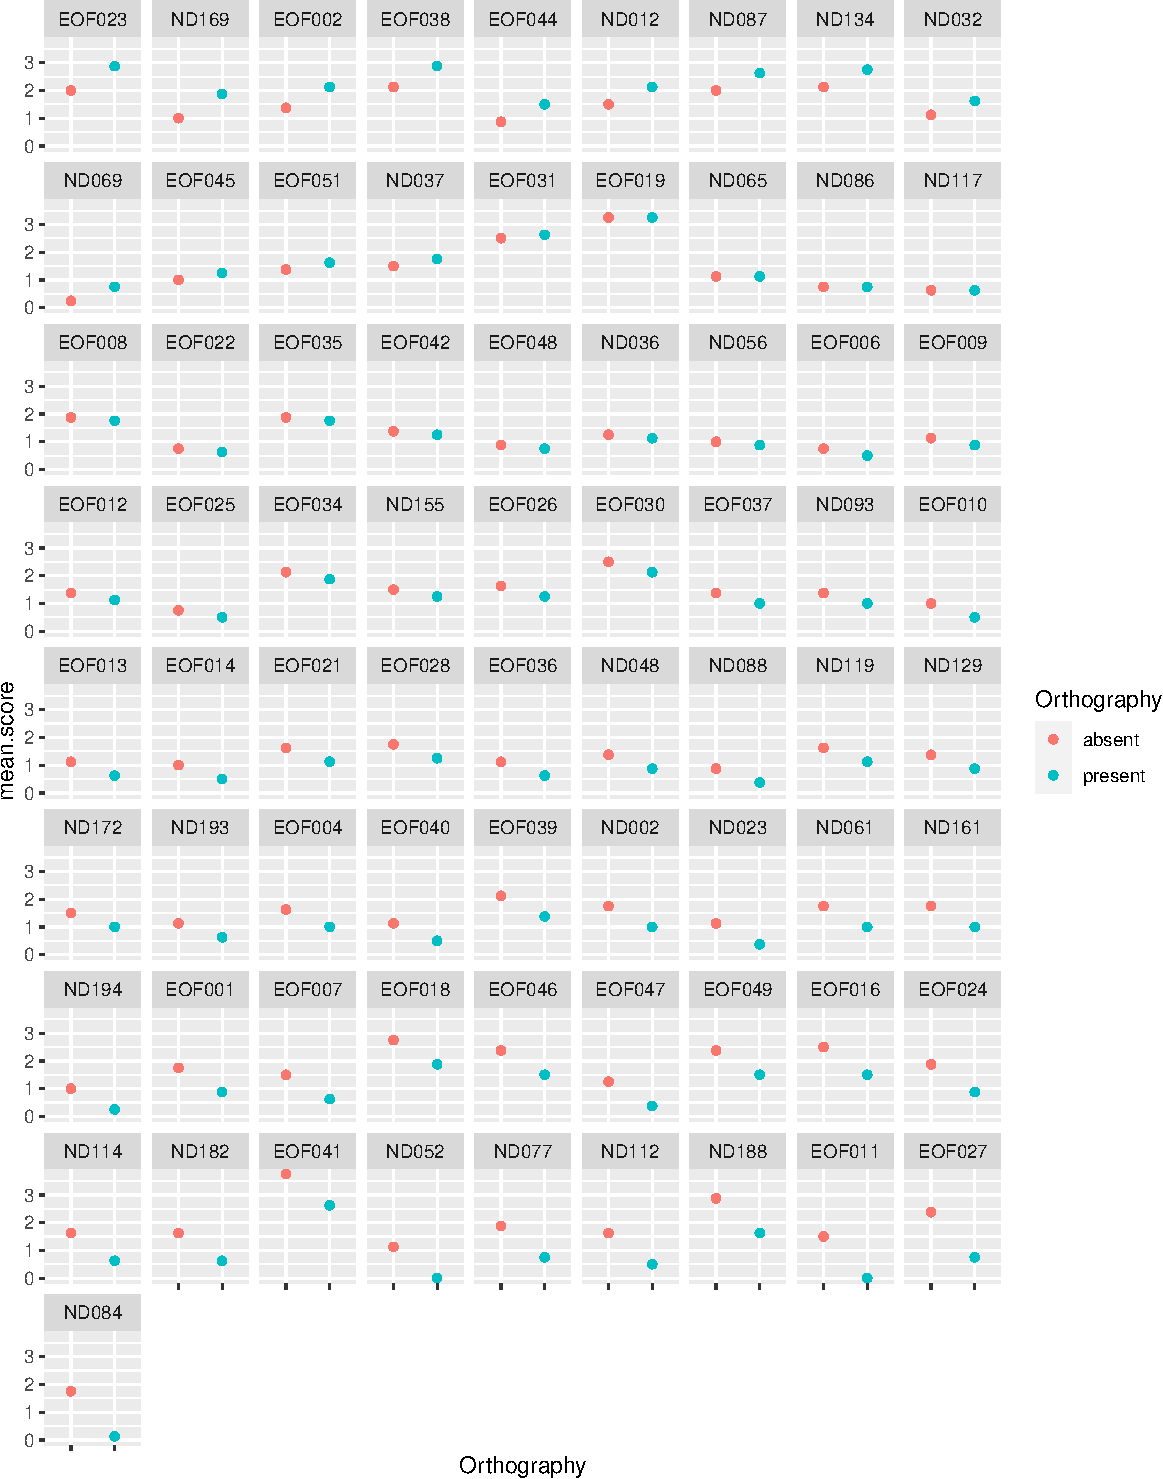
\includegraphics{visualization_files/figure-pdf/fig-effects-dot-facet-grid-effect-1.pdf}

}

\caption{\label{fig-effects-dot-facet-grid-effect}Dot plots showing the
different outcome spelling (Levenshtein) scores, for each participant,
in the different experimental conditions: Orthography (present, absent).
Plots are ordered, from top left to bottom right, by the difference
between mean spelling scores in the absent versus present conditions.}

\end{figure}

Once we have done the data processing in preparation, the code to
produce the plot is fairly compact.

\begin{enumerate}
\def\labelenumi{\arabic{enumi}.}
\tightlist
\item
  \texttt{ggplot(data\ =\ score.by.subj.diff\ ...} tells R to produce a
  plot, using \texttt{ggplot()} and the newly created
  \texttt{score.by.subj.diff} dataset.
\item
  \texttt{aes(x\ =\ Orthography,\ y\ =\ mean.score,...} specifies the
  aesthetic mappings: we tell R to locate \texttt{mean.score} on the
  y-axis and \texttt{Orthography} condition on the x-axis/
\item
  \texttt{aes(...colour\ =\ Orthography))\ +} specifies a further
  aesthetic mapping: we tell R to map different \texttt{Orthography}
  conditions to different colours.
\item
  \texttt{geom\_point()\ +} tells R to take the data and produce a
  scatterplot, given our mapping specifications.
\item
  \texttt{facet\_wrap(...)\ +} tells to split the dataset into sub-sets
  (facets).
\item
  \texttt{facet\_wrap(\textasciitilde{}\ reorder(Participant,\ difference.score))}
  tells R that we want the sub-sets to be organized by Participant, and
  we want the facets to be ordered by the \texttt{difference.score}
  calculated for each participant.
\item
  \texttt{theme(axis.text.x\ =\ element\_blank())} removes the x-axis
  labels because it is too crowded with the axis labels left in, and the
  information is already present in the colour guide legend shown on the
  right of the plot.
\end{enumerate}

\hypertarget{summary-visualizing-associations}{%
\subsection{Summary: Visualizing
associations}\label{summary-visualizing-associations}}

Visualizing associations between variables encompasses a wide range of
the things we have to do, in terms of both discovery and communication,
when we work with data from psychological experiments.

The conventional method to visualize how the distribution of values in
one variable covaries with the distribution of values in another
variable is through using a scatterplot. However, the construction of a
scatterplot can be elaborated in various ways to enrich the information
we present or communicate to our audiences, or to ourselves.

\begin{itemize}
\tightlist
\item
  We can add elements like smoothers to indicate trends.
\item
  We can add annotation, as with the histograms, to highlight specific
  thresholds.
\item
  We can facet the plots to indicate how trends may vary between
  sub-sets of the data.
\end{itemize}

In the final phases of our practical work, we started by presenting
model-based predictions of the effects of experimental manipulations.
However, you will have noticed that presenting plots of effects is not
where we stop when we engage with a dataset. Further plotting indicates
quite marked variation between participants in the effects of the
conditions. This kind of insight is something we can and should seek to
reveal through our visualization work.

\hypertarget{next-steps-for-development}{%
\section{Next steps for development}\label{next-steps-for-development}}

To take your development further, take a look at the resources listed in
Section~\ref{sec-resources}.

In my experience, the most productive way to learn about visualization
and about coding the production of plots, is by doing. And this work is
most interesting if you have a dataset you care about: for your research
report, or for your dissertation study.

As you have the alternate datasets described in
Section~\ref{sec-from-repros}, you can start with the data from the
other task or the other study in Ricketts et al. (2021). Ricketts et al.
(2021) recorded children's responses in two different outcome tasks, the
orthographic spelling task we have looked at, and a semantic or
meaning-based task. It would be a fairly short step to adapt the code
you see in the example code chunks to work with the semantic datasets.

Alternatively, you can look at the data reported by Rodríguez-Ferreiro
et al. (2020). Rodríguez-Ferreiro et al. (2020) present both measures of
individual differences (on schizotypyal traits) and experimental
manipulations (of semantic priming) so you can do similar things with
those data as we have explored here.

\hypertarget{sec-resources}{%
\section{Helpful resources}\label{sec-resources}}

\hypertarget{some-helpful-websites}{%
\subsection{Some helpful websites}\label{some-helpful-websites}}

\begin{itemize}
\tightlist
\item
  We typically use the \texttt{ggplot} library (part of the
  \texttt{tidyverse}) to produce plots. Clear technical information,
  with useful examples you can copy and run, can be found in the
  reference webpages:
\end{itemize}

\url{https://ggplot2.tidyverse.org/reference/index.html}

\begin{itemize}
\tightlist
\item
  A source of inspiration can be found here:
\end{itemize}

\url{https://r-graph-gallery.com}

If you are trying to work out how to do things by searching for
information online, you often find yourself at tutorial webpages. You
will develop a sense of quality and usefulness with experience. Most
often, what you are looking for is a tutorial that provides some
explanation, and example code you can adapt for your own purposes. Here
are some examples.

\begin{itemize}
\tightlist
\item
  Cedric Scherer on producing raincloud plots:
\end{itemize}

\url{https://www.cedricscherer.com/2021/06/06/visualizing-distributions-with-raincloud-plots-and-how-to-create-them-with-ggplot2/}

\begin{itemize}
\tightlist
\item
  Winston Chang on colours and colour blind palettes:
\end{itemize}

\url{http://www.cookbook-r.com/Graphs/Colors_(ggplot2)/}

\begin{itemize}
\tightlist
\item
  Thomas Lin Pedersen (and others) on putting together plots into a
  single presentation using the \texttt{patchwork} library functions:
\end{itemize}

\url{https://patchwork.data-imaginist.com/articles/patchwork.html}

\hypertarget{some-helpful-books}{%
\subsection{Some helpful books}\label{some-helpful-books}}

\begin{itemize}
\tightlist
\item
  The book ``R for Data Science'' (Wickham \& Grolemund, 2016) will
  guide you through the data analysis workflow, including data
  visualization, and the latest version can be accessed in an online
  free version here:
\end{itemize}

\url{https://r4ds.hadley.nz}

\begin{itemize}
\tightlist
\item
  The ``ggplot2: Elegant Graphics for Data Analysis'' book (Wickham,
  2016) corresponding to the \texttt{ggplot} library was written by
  Hadley Wickham in its first edition, it is now in its third edition
  (as a work in progress, co-authored by Wickham, Danielle Navarro and
  Thomas Lin Pedersen) and this latest version can be accessed in an
  online free version here:
\end{itemize}

\url{https://ggplot2-book.org/index.html}

\begin{itemize}
\tightlist
\item
  The ``R graphics cookbook'' (Chang, 2013), and the latest version can
  be accessed in an online free version here:
\end{itemize}

\url{https://r-graphics.org}

\begin{itemize}
\tightlist
\item
  The book ``Fundamentals of Data Visualization'' (Wilke, n.d.) is about
  different aspects of visualization, and can be accessed in an online
  free version here:
\end{itemize}

\url{https://clauswilke.com/dataviz/}

\part{THE RESEARCH REPORT ASSIGNMENT}

\bookmarksetup{startatroot}

\hypertarget{sec-report-intro}{%
\chapter{The research report assignment: Outline
introduction}\label{sec-report-intro}}

\begin{tcolorbox}[enhanced jigsaw, opacitybacktitle=0.6, title=\textcolor{quarto-callout-warning-color}{\faExclamationTriangle}\hspace{0.5em}{Warning}, arc=.35mm, colbacktitle=quarto-callout-warning-color!10!white, colframe=quarto-callout-warning-color-frame, leftrule=.75mm, opacityback=0, breakable, titlerule=0mm, left=2mm, bottomrule=.15mm, toprule=.15mm, colback=white, coltitle=black, bottomtitle=1mm, toptitle=1mm, rightrule=.15mm]

Under construction

\end{tcolorbox}

\bookmarksetup{startatroot}

\hypertarget{sec-intro-why}{%
\chapter{Reasons why we do the research report assignment: What you will
learn}\label{sec-intro-why}}

The research report assignment requires students to locate, access,
analyse and report previously collected data. This introduction is
intended to answer the first question anybody might ask.

\begin{itemize}
\tightlist
\item
  \textbf{Why}: what will you learn about, what is our motivation?
\end{itemize}

In following chapters, I will answer the questions.

\begin{itemize}
\tightlist
\item
  \textbf{What} do we expect students to do?
\item
  \textbf{How} can the assignment be done?
\end{itemize}

I hope you will agree that the discussion that follows is worth your
time in reading it. It will help you to understand \emph{why} we are
asking you to do the assignment, and \emph{why} we are looking for what
we are looking for. It will help you to understand \emph{how} this work
will aid your development.

You may not be interested in the discussion in this chapter. If you are
not, go ahead to the information on \textbf{what} we expect students to
do in Chapter~\ref{sec-what} and on \textbf{how} the work can be done in
Chapter~\ref{sec-how}.

\hypertarget{sec-why-key-ideas}{%
\section{The key ideas}\label{sec-why-key-ideas}}

There are two ideas motivating our approach. It will be helpful to you
if I sketch them out early, here. We can demonstrate the usefulness of
these ideas as we progress through our work.

The first key idea is expressed clearly in sociological discussions of
science. This is that there is a difference between science
``\ldots being done, science in the making, and science already done, a
finished product \ldots{}'' {[}Bourdieu (2004); p.2{]}. The awareness we
want to develop is that there are two things: there is the story that
may be presented in a textbook or in a lecture about scientific work or
scientific claims; and there is the work we do in practice, as we
develop graduate skills, and as we exercise those skills professionally
in the workplace.

The second key idea connects to the first. This idea is that reported
analyses are not \emph{necessary} or \emph{sufficient} to the data or
the question. What does this mean? It means that the same data can
reasonably be analysed in different ways. There is no \emph{necessary}
way to analyse some data though there may be conventions or normal
practices (Kuhn, 1970). It means that it is unlikely that any one
analysis will do all the work that could be done (a sufficiency) to get
you from your data to useful or reasonable answers to your questions.

These ideas may be unsettling but they are realistic. Stating them will
better prepare you for professional work. In the workplace, the accuracy
of these ideas will emerge when you see how a team in any sector
(health, marketing \ldots) gets from its data to its product. If we talk
about the ideas now, we can get you ready for dealing with the practical
and the ethical concerns you will confront when that happens.

We will begin by discussing psychological research, and research
\emph{about} psychological research, to answer the question:
\textbf{Why: what is the motivation for the assignment?} We will then
move to answering the \textbf{What} question Chapter~\ref{sec-what} and
the \textbf{How} question Chapter~\ref{sec-how}.

\hypertarget{sec-motivation-for-assignment}{%
\section{Why: what is the motivation for the
assignment?}\label{sec-motivation-for-assignment}}

\hypertarget{sec-wider-context-crises}{%
\subsection{The wider context: crisis and
revolution}\label{sec-wider-context-crises}}

We are here because we are interested in humans and human behaviour, and
because we are interested in scientific methods of making sense of these
things. Some of us are aware that science (including psychological
science) has undergone a rolling series of crises: the replicability or
replication crisis (Pashler \& Harris, 2012; Pashler \& Wagenmakers,
2012); the statistical crisis (A. Gelman \& Loken, 2014b); and the
generalizability crisis (Yarkoni, 2022). And that science is undergoing
a response to these crises, evidenced in the advocacy of
pre-registration (Nosek et al., 2018, 2019), and of registered reports
(Nosek \& Lakens, 2014), the use of open science badges (e.g.,
\href{https://www.psychologicalscience.org/publications/badges}{for the
journal \emph{Psychological Science}}), the completion of large-scale
replication studies (Aarts et al., 2015), and the identification of open
science principles (Munafò et al., 2017). We may usefully refer,
collectively, to the crises and the responses, as the \emph{credibility
revolution} (Vazire, 2018)

We could teach a course on this (in Lancaster, we do) but, here, I
invite you to follow the references if you are interested. Before going
on, I want to call your attention to the fact that important elements of
the hard work in trying to make science work better has been led by PhD
students and by junior researchers (e.g., Herndon et al., 2014).
Graduate students may, at first, assume that the fact that a research
article has been published in a journal means the findings that are
reported must be \emph{true}. Most of the time, some educated skepticism
is more appropriate. An important driver of the realization that there
are problems evident in the literature, and that there are changes we
can make to improve practice, comes from independent
\textbf{post-publication review work} exposing the problems in published
work (see, e.g.,
\href{https://statmodeling.stat.columbia.edu/2016/12/16/an-efficiency-argument-for-post-publication-review/}{this
account by Andrew Gelman})

\begin{tcolorbox}[enhanced jigsaw, opacitybacktitle=0.6, title=\textcolor{quarto-callout-tip-color}{\faLightbulb}\hspace{0.5em}{Tip}, arc=.35mm, colbacktitle=quarto-callout-tip-color!10!white, colframe=quarto-callout-tip-color-frame, leftrule=.75mm, opacityback=0, breakable, titlerule=0mm, left=2mm, bottomrule=.15mm, toprule=.15mm, colback=white, coltitle=black, bottomtitle=1mm, toptitle=1mm, rightrule=.15mm]

\begin{itemize}
\tightlist
\item
  Allow yourself to feel skeptical about the reports you read
  \emph{then} work with the motivation this feeling provides.
\end{itemize}

\end{tcolorbox}

In brief, then, most practicing scientists now understand \emph{or
should} understand that many of the claims we encounter in the published
scientific literature are unlikely to be supported by the evidence
(Ioannidis, 2005), whether we are looking at the evidence of the results
in the reports themselves, or evidence in later attempts to find the
same results (e.g., Aarts et al., 2015). We suspect that this may result
from a number of causes. We understand that researchers may engage in
questionable research practices (John et al., 2012). We understand that
researchers may exploit the potential for flexibility in doing and
reporting analyses (Simmons et al., 2011a). We understand that there are
problems in how psychologists use or talk about the measurement of
psychological constructs (Flake \& Fried, 2020). We understand that
there are problems in how psychologists sample people for their studies,
both in where we recruit (Bornstein et al., 2013; Henrich et al., 2010;
Wild et al., 2022), and in how many we recruit (Button et al., 2013;
Cohen, 1962; Sedlmeier \& Gigerenzer, 1989; Vankov et al., 2014). We
understand that there are problems in how psychologists specify or think
about their hypotheses or predictions (Meehl, 1967; Scheel, 2022). And
we understand that there are problems in how scientists do, or rather do
not, comply with good practice recommendations designed to fix these
problems (discussed further in the following).

This discussion could (again) be unsettling. This list of problems could
make you angry or sad. I, like others, think it is exciting. It is
exciting because these problems have probably existed for a long time
(e.g., Cohen, 1962; Meehl, 1967) but now, having identified the
problems, we can hope to do something about it. It is exciting because
if you care about people, the study of people, or the applications in
clinical, education and other domains of the results of the study of
people, then you might hope to see better, more useful, science in the
future (Vazire, 2018).

As someone who teaches graduate and undergraduate students, I want to
help you to \emph{be the change you want to see in the world}
\footnote{This encouragement is often attributed to Gandhi but is
  attributed
  (\href{https://professorbuzzkill.com/gandhi-be-the-change-you-wish-to-see-in-the-world/}{(here)})
  to a Brooklyn school teacher, Ms Arleen Lorrance, who led a
  transformative school project in the 1970s.}. We cannot solve every
problem but we can try to do better those things that are within our
reach. I am going to end this introduction with a brief discussion of
some ideas we can use to guide our better practices.

\hypertarget{sec-context-conceptual-practical}{%
\subsection{The specific context: what we need to look at, conceptually
and practically}\label{sec-context-conceptual-practical}}

In this course, for this assignment, we are going to focus on:

\begin{enumerate}
\def\labelenumi{\arabic{enumi}.}
\tightlist
\item
  multiverse analyses
\item
  kinds of reproducibility
\item
  the current state of the match between open science ideas and
  practices
\end{enumerate}

In the classes on the linear model, we will discuss:

\begin{enumerate}
\def\labelenumi{\arabic{enumi}.}
\setcounter{enumi}{3}
\tightlist
\item
  the links between theory, prediction and analysis
\item
  psychological measurement
\item
  samples
\item
  variation in results
\end{enumerate}

\hypertarget{sec-multi-what}{%
\subsection{\texorpdfstring{Multiverse analyses: \emph{multi-}
what?}{Multiverse analyses: multi- what?}}\label{sec-multi-what}}

\hypertarget{sec-pipeline}{%
\subsubsection{A first useful metaphor: the
pipeline}\label{sec-pipeline}}

I am going to link this discussion to a metaphor (see Figure
Figure~\ref{fig-pipeline}) or a description you will find useful:
\textbf{the data analysis pipeline} or \textbf{workflow}.

\begin{figure}

{\centering 

\begin{figure}[H]

{\centering \includegraphics[width=5in,height=3.5in]{intro_files/figure-latex/dot-figure-1.png}

}

\end{figure}

}

\caption{\label{fig-pipeline}The data analysis pipeline or workflow}

\end{figure}

This metaphor or way of thinking is very common
(\href{https://r4ds.had.co.nz/introduction.html}{take a look at the
diagram in Wickham and Grolemund's 2017 book ``R for Data Science}) and
you may see the words ``data pipeline'' used in job descriptions, or you
may benefit from saying, in a job application, something like: \emph{I
am skilled in designing and implementing each stage of the quantitative
data analysis pipeline, from data tidying to results presentation}. I
say this because scientists I have mentored got their jobs because they
can do these things -- and successfully explained that they can do these
things -- in sectors like educational testing, behavioural analysis, or
public policy research.

The reason this metaphor is useful is that it helps us to organize our
thinking, and to manage what we do when we do data analysis, we:

\begin{itemize}
\tightlist
\item
  get some data;
\item
  process or tidy the data;
\item
  explore, visualize, and analyse the data;
\item
  present or report our findings.
\end{itemize}

We introduce the idea that your analysis work will flow through the
stages of a \emph{pipeline} from getting the data to presenting your
findings because, next, we will examine how pipelines can
\emph{multiply}.

\begin{tcolorbox}[enhanced jigsaw, opacitybacktitle=0.6, title=\textcolor{quarto-callout-tip-color}{\faLightbulb}\hspace{0.5em}{Tip}, arc=.35mm, colbacktitle=quarto-callout-tip-color!10!white, colframe=quarto-callout-tip-color-frame, leftrule=.75mm, opacityback=0, breakable, titlerule=0mm, left=2mm, bottomrule=.15mm, toprule=.15mm, colback=white, coltitle=black, bottomtitle=1mm, toptitle=1mm, rightrule=.15mm]

\begin{itemize}
\tightlist
\item
  As you practice your data analysis work, try to identify the elements
  and the order of your work, as the parts of a \emph{workflow}.
\end{itemize}

\end{tcolorbox}

\hypertarget{sec-forking}{%
\subsubsection{A second useful metaphor: the garden of forking
paths}\label{sec-forking}}

What researchers have come to realize: because we started looking
\ldots{} The open secret that has been well kept (Bourdieu, 2004):
because everybody who does science knows about it, yet we may not teach
it; and because we do not write textbooks revealing it \ldots{} Is that
at each stage in the analysis workflow, we can and do make choices where
multiple alternative choices are possible. A. Gelman \& Loken (2014a)
capture this insight as the ``garden of forking paths''\footnote{The
  term is taken from the name of a short story by Jorge Luis Borges,
  ``El jardin de senderos que se bifurcan'' (translated as `The garden
  of forking paths').} (see Figure~\ref{fig-forking}).

The general idea is that it is possible to have \textbf{multiple
potential different paths} from the data to the results. The results
will vary, depending on the path we take. In an analysis, we could take
multiple different paths simply because at point A we decide to do B1,
B2 or B3, maybe we choose B1, and then at point B1, we may decide to do
C1, C2 or C3. Here, maybe we have our raw data at point A. Maybe we
could do one of two different things when we tidy the data: action B1 or
B2. Then, when we have our tidy data, maybe we can choose to do our
analysis in one of six ways. Where we are at each step \emph{depends} on
the choices we made at the previous steps.

\begin{figure}

{\centering 

\begin{figure}[H]

{\centering \includegraphics[width=5in,height=3.5in]{intro_files/figure-latex/dot-figure-2.png}

}

\end{figure}

}

\caption{\label{fig-forking}Forking paths in data analysis}

\end{figure}

In the end, it may appear to us that we took one path or that only one
path was possible. When we report our analysis, in a dissertation or in
a published journal article, we may report the analysis \textbf{as if
only one analysis path had been considered}. But, critically, our
findings may depend on the choices we made and this variation in results
may be hidden from view.

I am talking about forking paths because the \emph{multiplicity} of
paths has consequences, and we discuss these next.

\begin{tcolorbox}[enhanced jigsaw, opacitybacktitle=0.6, title=\textcolor{quarto-callout-tip-color}{\faLightbulb}\hspace{0.5em}{Tip}, arc=.35mm, colbacktitle=quarto-callout-tip-color!10!white, colframe=quarto-callout-tip-color-frame, leftrule=.75mm, opacityback=0, breakable, titlerule=0mm, left=2mm, bottomrule=.15mm, toprule=.15mm, colback=white, coltitle=black, bottomtitle=1mm, toptitle=1mm, rightrule=.15mm]

\begin{itemize}
\tightlist
\item
  It is about here, I hope, that you can start to see why it would makes
  sense to access data from a published study and to examine if you can
  get the same results as the study authors.
\end{itemize}

\end{tcolorbox}

\hypertarget{sec-multiverse}{%
\subsection{Multiverse analyses}\label{sec-multiverse}}

I am going to discuss, now, what are commonly called \emph{multiverse
analyses}. Psychologists use this term, having been introduced to it in
an influential paper by Steegen et al. (2016a), but it comes from
theoretical physics
(\href{https://en.wikipedia.org/wiki/Multiverse}{take a look at
wikipedia}).

I explain this because I do not want you to worry. The ideas themselves
are within your grasp whatever your background in psychology or
elsewhere. It is the implications for our data analysis practices that
are \emph{challenging}. They are challenging because what we discuss
should increase your skepticism about the results you encounter in
published papers. And they are challenging because they \emph{reveal
your freedom} to question whether published authors could have done
their analysis in a different way.

We are going to look at:

\begin{enumerate}
\def\labelenumi{\arabic{enumi}.}
\tightlist
\item
  data-set construction
\item
  analysis choices
\end{enumerate}

\hypertarget{the-link-between-the-credibility-revolution-and-the-multiverse}{%
\subsubsection{The link between the credibility revolution and the
multiverse}\label{the-link-between-the-credibility-revolution-and-the-multiverse}}

In first discussing the wider context (of crisis and revolution), then
discussing the specific context (of multiverses and, in the following,
of reproducibility), I should be clear about \textbf{the link between
the two things}. The finding that some results may not be supported by
the evidence is probably due to a mix of causes. But one of those causes
will be the combination of uncertainty over data processing or the
uncertainty over analysis methods revealed in multiverse analyses, as we
see next, combined with the limitations of data and code sharing, and
the incompleteness of results reporting (as we see later).

\hypertarget{sec-multiversedata}{%
\subsubsection{The data multiverse}\label{sec-multiversedata}}

When you collect or access data for a research study, the complete raw
data-set you receive is almost never the complete data-set you analyse
or whose analysis you report. This is not a story about deliberately
cheating. It is a story about the normal practice of science (Kuhn,
1970).

Picture some common scenarios. You did a survey, you got responses from
a 100 participants on 10 questions, and you asked people to report their
education, ethnicity and gender. You did an experimental study, you
tested two groups of 50 people each in 100 trials (imagine a common task
like the Stroop test), and you observed the accuracy and the timing of
their responses. You tested 100 children, 20 children in each of five
different schools, on a range of educational ability measures.

In these scenarios, the psychologist or the analyst of behavioural data
\emph{must} process their data. In doing so, you will ask yourself a
series of questions like:

\begin{itemize}
\tightlist
\item
  how do we code for \texttt{gender,\ ethnicity,\ education}?
\item
  what do we about reaction times that are very short, e.g.,
  \(RT < 200ms\) or very long, e.g., \(RT > 1500ms\))?
\item
  if we present multiple questions measuring broadly the same thing
  (e.g.~how confident are you that you understand what you have read?
  how easy did you find what you read?) how do we summarize the scores
  on those questions? do we combine scores?
\item
  what do we do about people who may not appear to have understood the
  task instructions?
\end{itemize}

Typically, the answers to these questions will be given to you by your
supervisor, a colleague or a textbook example. For example, we might
say:

\begin{itemize}
\tightlist
\item
  ``We excluded all reaction times greater than 1500ms before
  analysis.''
\end{itemize}

Typically, the explanation for these answers are rarely explained. We
might say:

\begin{itemize}
\tightlist
\item
  ``\emph{Consistent with common practice in this field}, we excluded
  all reaction times greater than 1500ms before analysis.''
\end{itemize}

But the reader of a journal article typically \textbf{will not see} an
explanation for why, as in the example, we exclude reaction times
greater than 1500ms and not 2000ms or 3000ms, etc. We typically do not
see an explanation for why \emph{we} exclude all reaction times greater
than 1500ms but \emph{other} researchers exclude all reaction times
greater than 2000ms. (I do not pick this example at random: there are
serious concerns about the impact on analyses of exclusions like this
(Ulrich \& Miller, 1994).)

What Steegen et al. (2016a) showed is that a data-set can be processed
for analysis in multiple different ways, with a number of reasonable
alternate choices that can be applied, for each choice point:
construction choices about classifying people or about excluding
participants given their responses. If a different data-set is
constructed for each combination of alternatives then many different
data-sets can be produced, all starting from the same raw data. (For
their example study, Steegen et al. (2016a) found they could construct
120 or 210 different data-sets, based on the choice combinations.)
Critically, for us, Steegen et al. (2016a) showed that if we apply the
same analysis method to the different data-sets then our results will
vary.

Let me spell this out, bit by bit:

\begin{itemize}
\tightlist
\item
  we approach our study with the same research question, and the same
  verbal prediction;
\item
  we begin with the exact same data;
\item
  we then construct different data-sets depending on different \emph{but
  equally reasonable} processing choices;
\item
  we then apply the same analysis analysis, to test the same prediction,
  using each different data-set;
\item
  we will see different results for the analyses of the different
  data-sets.
\end{itemize}

Alternate constructions of the same data may cause variation in the
results of statistical tests. Some kinds of data processing choices may
be more influential on results than others. It seems unlikely that we
can identify, in advance, which choices matter more.

Steegen et al. (2016a) suggest that we can \emph{deflate} (shrink) the
multiverse in different ways. I want to state their suggestions, here,
because we will come back to these ideas in the classes on the linear
model.

\begin{enumerate}
\def\labelenumi{\arabic{enumi}.}
\tightlist
\item
  Develop better theories and improved measurement of the constructs of
  interest.
\item
  Develop more complete and precise theory for why some processing
  options are better than others.
\end{enumerate}

But you will be asking yourself: \textbf{What do I need to think about,
for the research report assignment?}

\begin{tcolorbox}[enhanced jigsaw, opacitybacktitle=0.6, title=\textcolor{quarto-callout-tip-color}{\faLightbulb}\hspace{0.5em}{Tip}, arc=.35mm, colbacktitle=quarto-callout-tip-color!10!white, colframe=quarto-callout-tip-color-frame, leftrule=.75mm, opacityback=0, breakable, titlerule=0mm, left=2mm, bottomrule=.15mm, toprule=.15mm, colback=white, coltitle=black, bottomtitle=1mm, toptitle=1mm, rightrule=.15mm]

\begin{itemize}
\tightlist
\item
  When you read a psychological research report, identify where the
  researchers talk about how they process their data: classification,
  coding, exclusion, transformation, etc.
\item
  If you can access the raw data, ask yourself: could different choices
  change the results of the same analysis?
\end{itemize}

\end{tcolorbox}

\hypertarget{sec-multiverseanalysis}{%
\subsubsection{Analysis multiverses}\label{sec-multiverseanalysis}}

Even if we begin with the same research question and, critically, the
\emph{same data-set}, the results of a series of studies show that
different researchers will often (reasonably) make \emph{different
choices about the analysis} they do to answer the research question. We
often call these studies (analysis or model) \textbf{multiverse}
studies. In these studies, we see variation in analysis and this
variation is also associated with variation in results.

An influential example, in psychology, is reported by Silberzahn and
colleagues (Silberzahn et al., 2017; Silberzahn \& Uhlmann, 2015) who
asked 29 teams of researchers to answer the same question (``Are
(soccer) referees more likely to give red cards to players with dark
skin than to players with light skin?'') with the same data-set (data
about referee decisions in football league games). The teams made their
own decisions about how to answer the question in doing the analysis.
The teams shared their plans, and commented on each others' ideas. The
discussion did not lead to a consensus about what analysis approach is
best. In the end, the different teams did different analyses and,
critically, the \textbf{different analyses had different results}. The
results varied in whether the test of the effect of players skin colour
(on whether red cards were given) was significant or not, and on the
strength of the estimated association between the darkness of skin
colour (lighter to darker) and the chances (low to high) of getting a
red card.

There have now been a series of multiverse or multi-analyst studies
which demonstrate that, under certain conditions, different researchers
may adopt different analysis approaches -- which will have
\emph{different results} -- in answering the same research question with
the same data. This demonstration has been repeated in studies in
health, medicine, psychology, neuoscience, and sociology, among other
research fields (e.g., Parsons (n.d.); Breznau et al. (2022); Klau et
al. (n.d.); Klau et al. (2021); Wessel et al. (2020); Poline et al.
(2006); Maier-Hein et al. (2017); Starns et al. (2019); Fillard et al.
(2011); Dutilh et al. (2019); Salganik et al. (2020); Bastiaansen et al.
(2020); Botvinik-Nezer et al. (2020); Schweinsberg et al. (2021); Patel
et al. (2015); see, for reviews, and some helpful guidance, Aczel et al.
(2021); Del Giudice \& Gangestad (2021); Hoffmann et al. (n.d.);
Wagenmakers et al. (2022)).

In these studies, we typically see variation in how psychological
constructs are operationalized (e.g., how do we measure or code for
social status?), how data are processed or data-sets constructed (as in
Steegen et al. (2016b)), plus variation in \emph{what} statistical
techniques are used, and in \emph{how} those techniques are used. This
variation can be understood to reflect kinds of \textbf{uncertainty}
(Klau et al., n.d.; Klau et al., 2021): uncertainty about how to process
data, and uncertainty about the model or methods we should use to test
or estimate effects. Further research makes it clear that we should be
aware, if we are not already, of the variation in results that can be
expected because different researchers may choose to design studies, and
construct stimulus materials, in different ways given the same research
hypothesis information (Landy et al., 2020).

But you will be asking yourself: \textbf{What do I need to think about,
for the research report assignment?}

\begin{tcolorbox}[enhanced jigsaw, opacitybacktitle=0.6, title=\textcolor{quarto-callout-tip-color}{\faLightbulb}\hspace{0.5em}{Tip}, arc=.35mm, colbacktitle=quarto-callout-tip-color!10!white, colframe=quarto-callout-tip-color-frame, leftrule=.75mm, opacityback=0, breakable, titlerule=0mm, left=2mm, bottomrule=.15mm, toprule=.15mm, colback=white, coltitle=black, bottomtitle=1mm, toptitle=1mm, rightrule=.15mm]

\begin{itemize}
\tightlist
\item
  When you read a psychological research report, identify where the
  researchers talk about how they analyse their data: the hypothesis or
  prediction they test; the method; their assumptions; the variables
  they include; the checks or the alternate analyses they did or did not
  do.
\item
  If you can access the data and analysis code, ask yourself: could
  different methods change the results of the same analysis?
\end{itemize}

\end{tcolorbox}

\hypertarget{what-can-we-conclude-the-story-so-far}{%
\subsubsection{What can we conclude -- the story so
far?}\label{what-can-we-conclude-the-story-so-far}}

This is a good place to look at what we have discussed, and present an
evaluation of the story so far.

This is not a story where everybody or nobody is right or where
everything or nothing is true \footnote{There could be a story where the
  hero (us) ultimately learns to reject binary (present, absent;
  significant, non-significant) choices, and embrace variation, or
  embrace uncertainty (a. Gelman, 2015; Vasishth \& Gelman, 2021).}.
Instead, we can be guided by the advice (Meehl, 1967; Scheel, 2022;
Steegen et al., 2016a) that we should:

\begin{enumerate}
\def\labelenumi{\arabic{enumi}.}
\tightlist
\item
  seek better and more complete theorizing about the constructs of
  interest and how we measure them, and
\item
  seek more complete and more precise theory so that some options are
  theoretically superior than others, and should be preferred, when
  constructing data-sets or specifying analysis methods.
\end{enumerate}

Not all research questions and not all hypothesis information will allow
an equally wide variety of potential reasonable approaches to the
analysis. As Paul Meehl argued a long time ago (Meehl, 1967, 1978), and
researchers like Anne Scheel (Scheel et al., 2021; Scheel, 2022) argued
more recently, the complexity of the thing we study -- people, and what
they do -- and the still early development of our understanding of this
thing, mean that what we \emph{want} but what we do not see, in
psychology, are scientifically productive tests of \emph{falsifiable
theories}. (See, consistent with this perspective, discussions by
Auspurg \& Brüderl (2021) and by Del Giudice \& Gangestad (2021) about
the range of analysis possibilities that may or may not be allowed, in
multiverse analyses, by more or less clear research questions or
well-developed causal theories.) Our concern should not so much be with
being able to do statistical analysis, or with finding significant or
not significant results. It would be more useful to do analyses to test
concrete, inflexible, precise predictions that \emph{can be wrong}.

Nor is this a story, I think, about the potential for \emph{cheating}.
While we may refer to subjective choices or to researcher flexibility,
the differences that we see do not resemble the \emph{researcher degrees
of freedom} (Simmons et al., 2011b) some may exploit, consciously or
unconsciously, to change results to suit their aims. Instead, the
multiverse results show us the impact of the reasonable differences in
approach that different researchers may sensibly choose to take when
they try to answer a research question with data.

Not all alternates, at a given point of choosing, in the data analysis
workflow, will have equal impact. Work by Young (Young, 2018; Young \&
Holsteen, 2017) indicates that if we deliberately examine the impact of
method or model uncertainty, over different sets of possible choices ---
about what variables or what observations we include in an analysis, for
example --- we may find that some results are robust to an array of
different options, while other results are highly susceptible to
different choices. This work suggests another way in which uncertainty
about methods or variation in results can be turned into progress in
understanding the phenomena that interest us: through systematic,
informed, interrogation of the ways that results can vary.

In general, in science, the acceptance of research findings must always
be negotiated (Bourdieu, 2004). Here, we see that the grounds of
negotiation should often include an analysis of the impact on the value
of evidence of the different analysis approaches that researchers can or
do apply to the data that underlie that evidence.

But you will be asking yourself: \textbf{what do I need to think about,
for the assignment?}

\begin{tcolorbox}[enhanced jigsaw, opacitybacktitle=0.6, title=\textcolor{quarto-callout-tip-color}{\faLightbulb}\hspace{0.5em}{Tip}, arc=.35mm, colbacktitle=quarto-callout-tip-color!10!white, colframe=quarto-callout-tip-color-frame, leftrule=.75mm, opacityback=0, breakable, titlerule=0mm, left=2mm, bottomrule=.15mm, toprule=.15mm, colback=white, coltitle=black, bottomtitle=1mm, toptitle=1mm, rightrule=.15mm]

\begin{itemize}
\tightlist
\item
  The results of multiverse analyses show us that if we see one analysis
  reported in a paper, or one workflow, that does not mean that only one
  analysis can reasonably be applied.
\item
  If you read the methods or results section of a paper, you should
  reflect: what other analysis methods could be used here? How could
  variation in analysis method --- in what or how you do the analysis
  --- influence the results?
\end{itemize}

\end{tcolorbox}

Making you aware of the potential for analysis choices is useful because
developing researchers, including graduate students, are often not aware
of the room for choice in the data analysis workflow. Developing
researchers --- you --- may be instructed that ``this is how we do
things'' or ``you should follow what researchers did previously''.
Following convention is not necessarily a bad thing: it is a feature of
the normal practice of science (Kuhn, 1970). However, you can now see,
perhaps, that there likely will be alternative ways to process or to
analyse data than the approach a supervisor, lab or field normally
adopts.

This understanding or awareness has three implications for practice, it
means:

\begin{enumerate}
\def\labelenumi{\arabic{enumi}.}
\tightlist
\item
  When we talk about the analysis we do, we should explain our choices.
\item
  We should check, or enable others to check, what impact making
  different choices would have on our results.
\item
  Most importantly: \textbf{we can allow ourselves the freedom to
  critically evaluate} the choices researchers make, even the choices
  researchers make in published articles.
\end{enumerate}

\hypertarget{from-the-multiverse-to-kinds-of-reproducibility}{%
\subsection{From the multiverse to kinds of
reproducibility}\label{from-the-multiverse-to-kinds-of-reproducibility}}

Multiverse analyses and post-publication analyses, in general, show that
we can and should question or critically evaluate the analyses we
encounter in the literature. This work can usefully detect problems in
original published analyses (e.g., A. Gelman \& Weakliem, 2009; Herndon
et al., 2014; Wagenmakers et al., 2011). It can demonstrate where
original published claims are or are not robust to variation of analysis
method or approach.

Given these lessons, and the implications we have identified, we should
expect or hope to see open science practices (Munafò et al., 2017; Nosek
et al., 2022):

\begin{itemize}
\tightlist
\item
  share data and code;
\item
  publish research reports in ways that enable others to check or query
  analyses.
\end{itemize}

As we discuss, following, these practices are now common but the quality
of practice can sometimes be questioned. This matters for you because it
makes it more challenging -- in specific identifiable locations -- to
locate, access, analyse and report previously collected data.

The discussion of current practices identifies where or how the
assignment may be more challenging, but also identifies some of the
exact places where the assignment provides \textbf{a real opportunity to
do original research work}.

First, I am going to introduce some ideas that will help you to think
about what you are doing when you do this work. We focus on the concept
of \emph{reproducibility}.

Gilmore et al. (2017; following Goodman et al., 2016) present three
kinds of reproducibility:

\begin{itemize}
\tightlist
\item
  methods reproducibility
\item
  results reproducibility
\item
  inferential reproducibility
\end{itemize}

In looking at reproducibility, here, we are considering how much, or in
what ways, the results or the claims that are made in a published study
can be found or \emph{repeated} by someone else.

\hypertarget{sec-methodsrepro}{%
\subsubsection{Methods reproducibility}\label{sec-methodsrepro}}

As Gilmore et al. (2017) discuss, \textbf{methods reproducibility} means
that another researcher should be able to get the same results if they
use the same tools and analysis methods to analyse the same data-set
{[}some researchers also refer to \emph{analytic reproducibility} or
\emph{computational reproducibility}; see e.g. Crüwell et al. (n.d.);
Hardwicke et al. (2018); Hardwicke et al. (n.d.); Laurinavichyute et al.
(2022); Minocher et al. (n.d.){]}.

In neuroimaging, the multiplicity of possible implementations of the
data analysis pipeline (Carp, 2012a), and the fact that important
elements or information about the pipeline deployed by researchers may
be missing from published reports (Carp, 2012b), can make it challenging
to identify how results can be reproduced.

In psychological science, in evaluating reports of results from analyses
of behavioural data collected through survey or experimental work, in
principle, we should expect to be able to access the data collected by
the study authors, follow the description of their analysis method, and
reproduce the results they report.

\begin{tcolorbox}[enhanced jigsaw, opacitybacktitle=0.6, title=\textcolor{quarto-callout-tip-color}{\faLightbulb}\hspace{0.5em}{Tip}, arc=.35mm, colbacktitle=quarto-callout-tip-color!10!white, colframe=quarto-callout-tip-color-frame, leftrule=.75mm, opacityback=0, breakable, titlerule=0mm, left=2mm, bottomrule=.15mm, toprule=.15mm, colback=white, coltitle=black, bottomtitle=1mm, toptitle=1mm, rightrule=.15mm]

\begin{itemize}
\tightlist
\item
  For an assignment in which we ask students to locate, access, analyse
  and report previously collected data, we are directly concerned with
  \emph{methods reproducibility}.
\end{itemize}

\end{tcolorbox}

\hypertarget{sec-resultsrepro}{%
\subsubsection{Results reproducibility}\label{sec-resultsrepro}}

\textbf{Results reproducibility} means that if another researcher
completes a new study with new data they are able to get the same
results as the results reported following an original study: this often
referred to as \emph{replication}. The replication studies that have
been reported (e.g., Aarts et al., 2015), and continue to be reported
(see, for example, the studies discussed by Nosek et al. (2022)), in the
last several years, present attempts to examine the results
reproducibility of published findings.

In the classes on the linear model, we will examine if similar or
different results are observed in a series of studies using the same
procedure and the same materials. We shall discuss, in those classes, in
more depth, what results reproducibility (or study replication) can or
cannot tell us about the behaviours that interest us.

\hypertarget{sec-inferencerepro}{%
\subsubsection{Inferential reproducibility}\label{sec-inferencerepro}}

\textbf{Inferential reproducibility} means that if a researcher repeats
a study (aiming for results reproducibility) or re-analyses an original
data-set (aiming for methods reproducibility) then they can come to the
same or similar conclusions as the authors of the report of an original
study.

How is inferential reproducibility not methods or results
reproducibility? Goodman et al. (2016) explain that researchers can make
the same conclusions from different sets of results and \emph{can reach
different conclusions from the same set of results}.

How is it possible to reach different conclusions from the same results?
We can imagine two scenarios.

First, we have to think about the wider research field, the research
context, within which we consider a set of results. It may be that two
different researchers will come to look at the same results with
different expectations about what the results \emph{could} tell us (in
Bayesian terms, with different prior expectations). Given different
expectations, it is easy to imagine different researchers looking at the
same results and, for example, one researcher being more skeptical than
another about what conclusion can be taken from those results. (In the
class on graduate writing skills, I discuss in some depth the importance
of reviewing a research literature in order to get an understanding of
the assumptions, conventions or expectations that may be shared by the
researchers working in the field.)

Second, imagine two different researchers looking at the same results
--- picture the original authors of a published study, and someone doing
a post-publication re-analysis of their data --- you can expect that the
re-analysis or the reproducibility analysis could identify reasons to
value the evidence differently, or to reach more skeptical conclusions,
through critical evaluation of:

\begin{itemize}
\tightlist
\item
  data processing choices;
\item
  the choice of the method used to do analysis;
\item
  choices in how the analysis method is used.
\end{itemize}

\ldots{} where that critical evaluation involves an analysis of the
choices the original researchers made, perhaps involving an analysis of
other choices they could have made, perhaps reflecting on how
effectively the analyses address a given research question or test a
given prediction.

\begin{tcolorbox}[enhanced jigsaw, opacitybacktitle=0.6, title=\textcolor{quarto-callout-tip-color}{\faLightbulb}\hspace{0.5em}{Tip}, arc=.35mm, colbacktitle=quarto-callout-tip-color!10!white, colframe=quarto-callout-tip-color-frame, leftrule=.75mm, opacityback=0, breakable, titlerule=0mm, left=2mm, bottomrule=.15mm, toprule=.15mm, colback=white, coltitle=black, bottomtitle=1mm, toptitle=1mm, rightrule=.15mm]

\begin{itemize}
\tightlist
\item
  We can think about the work we do, when we analyse previously reported
  data, in terms of the need to identify the \emph{reproducibility} of
  results, methods and inferences.
\item
  In psychological science, determining that someone can get the same
  results, by analysing the same data, or will reach the same
  conclusions from the same results, are important -- potentially,
  original -- research contributions.
\end{itemize}

\end{tcolorbox}

\hypertarget{the-current-state-of-the-match-between-open-science-ideas-and-practices}{%
\subsection{The current state of the match between open science ideas
and
practices}\label{the-current-state-of-the-match-between-open-science-ideas-and-practices}}

I have said that we should expect or hope to see open science practices
(Munafò et al., 2017; Nosek et al., 2022) where researchers:

\begin{itemize}
\tightlist
\item
  share data and code;
\item
  publish research reports in ways that enable others to check or query
  analyses.
\end{itemize}

This raises an important question: \textbf{What exactly do we see, when
we look at current practices?} The question is important because
answering it helps to identify where the challenges are located when you
complete your work to locate, access, analyse and report previously
collected data.

I break the discussion of what we see into two parts. Firstly, I look at
the results of audits of data and code sharing (see
Section~\ref{sec-sharing}): are data shared and can we access the data?
Secondly, I discuss analyses of methods reproducibility, and shared data
and code usability (see Section~\ref{sec-checkanalyses}): can others
reproduce the results reported in published articles, given shared data?
can others access and run shared analysis code? can others use the
shared code to reproduce the reported results? Again, I need to be brief
but reference sources that you can follow-up.

\hypertarget{the-link-between-the-credibility-revolution-and-the-reproducibility-of-results}{%
\subsubsection{The link between the credibility revolution and the
reproducibility of
results}\label{the-link-between-the-credibility-revolution-and-the-reproducibility-of-results}}

I should be clear, before we go on, about \textbf{the link} between the
\emph{credibility revolution} in science, and the effort to examine
reproducibility of results. Many elements of the credibility revolution
emerged out of the observation that it has often been difficult to
repeat the results of published studies when we conduct new studies
(replication studies or results reproducibility; e.g., Aarts et al.
(2015)). However, it is clearly difficult to know \emph{what} to
replicate or reproduce if we cannot reproduce the results presented in a
study report (methods reproducibility), given the study data (Artner et
al., 2021; Laurinavichyute et al., 2022; Minocher et al., n.d.).

\hypertarget{sec-sharing}{%
\subsubsection{Data and code sharing}\label{sec-sharing}}

Research on data and code sharing practices suggest that practices have
improved, from earlier low levels.

In an important early report, Wicherts et al. (2006) observed that it
was very difficult to obtain data reported in psychological research
articles from the authors of the articles. They asked for data from the
lead authors of 141 articles published in four leading psychology
journals, for about 25\% of the studies. This low response rate was
found despite the fact that authors in these journals must agree to the
principle that data can be shared with others wishing to verify claims.

Practice \emph{has} changed: how?

One change to practice has involved the use of \textbf{open science
badges}. In journals like
\href{https://www.psychologicalscience.org/publications/badges}{Psychological
Science} authors of articles may be awarded badges --- Open Data, Open
Materials, Preregistration badges --- by the editorial team. Authors can
apply for and earn the badges by providing information about open
practices, and journal articles are published with the badges displayed
near the front of the articles.

In theory, initiatives like encouraging authors to earn open science
badges should mean that data sharing practices improve, enabling access
to data and code for those, like you, who would like to re-analyse
previously published data. In theory, all you should need to do --- to
locate and access data --- is just search articles in the journal
\emph{Psychological Science} for studies with open data badges, and
follow links from the published articles to then access study data at an
open repository like the \emph{Open Science Framework}
\href{https://osf.io}{(OSF)} What do we see in practice?

Analyses reported by Kidwell et al. (2016) as well as analyses reviewed
by Nosek et al. (2022) indicate that more articles have claimed to make
data available in the time since badges were introduced. When they did
their analysis, Kidwell et al. (2016) found that a substantial
proportion, but not all, of the articles in \emph{Psychological Science}
can be found to actually provide access to shared data. However,
critically, many but not all the articles with open data badges provide
access to data available through an open repository, data that are
correct, complete and usable (Kidwell et al., 2016). In their later
report, the analyses reviewed by Nosek et al. (2022) suggest that the
use of repositories like OSF for data sharing may be accelerating but
that, over the last few years, the rate at which open science practices
like sharing data, overall, appears to be substantial but not yet
reported or observed in a majority of the work of researchers.

Many journals now require the authors of articles to include a
\textbf{Data Availability Statement} to locate their data. Analyses by
Federer (2022) indicate that Data Availability Statements for articles
published in the open access \footnote{Open access journals publish
  articles that are free to read or download.} journal PLOS ONE often,
helpfully, include Digital Object Identifiers (DOIs) or Universal
resource locators (URLs) enabling direct access to shared data (i.e.,
without having to contact authors). Of those DOIs or URLs, most appeared
to be associated with resources that could successfully be retrieved. In
contrast, analyses reported by Gabelica et al. (2022) indicate that
where article authors state that ``data sets are available on reasonable
request'' (the most common availability statement), most of the time,
the authors did not respond or declined to share the data (see similar
findings, across fields, by Tedersoo et al., 2021). Clearly, in the
analyses of open science practices we have seen so far, data sharing is
more effective where sharing does not have to work through authors.

\begin{tcolorbox}[enhanced jigsaw, opacitybacktitle=0.6, title=\textcolor{quarto-callout-tip-color}{\faLightbulb}\hspace{0.5em}{Tip}, arc=.35mm, colbacktitle=quarto-callout-tip-color!10!white, colframe=quarto-callout-tip-color-frame, leftrule=.75mm, opacityback=0, breakable, titlerule=0mm, left=2mm, bottomrule=.15mm, toprule=.15mm, colback=white, coltitle=black, bottomtitle=1mm, toptitle=1mm, rightrule=.15mm]

\begin{itemize}
\tightlist
\item
  When you are looking for a study in order to get data that you can
  then re-analyse, it makes sense to look, first, for studies focusing
  on research questions that interest you.
\item
  When you are looking for published reports where the authors share
  data, look for articles with open science badges or where you can see
  a Data Availability Statement.
\item
  Choose articles where the authors provide a direct link to their data,
  where the data are located on an open repository like the Open Science
  Framework (there are other repositories).
\end{itemize}

\end{tcolorbox}

\hypertarget{sec-checkanalyses}{%
\subsubsection{Enabling others to check or query
analyses}\label{sec-checkanalyses}}

Research on data and code sharing practices suggest that practices have
improved but that there are concerns about the quality of the sharing.
Here, the critical concern relates to the word \emph{enable} in the
objective: that we should publish research reports in ways that
\emph{enable} others to check or query analyses.

John Towse and colleagues (Towse et al., 2021) at Lancaster University
examined the quality of open data-sets to assess their quality in terms
of their completeness and reusability (see also Roche et al., 2015).

\begin{itemize}
\tightlist
\item
  \textbf{completeness}: are all the data and the data descriptors
  supporting a study's findings publicly available?
\item
  \textbf{reusability}: how readily can the data be accessed and
  understood by others?
\end{itemize}

For a sample of data-sets, they found that about half were incomplete,
and about two-thirds were shared in a way that made them difficult to
use. Practices tended to be slightly better in more recent publications.
(Broadly similar results are reported by (Hardwicke et al., 2018).)

Where data were found to be incomplete, this appeared to be, in part,
because participants were excluded in the processing of the data for
analysis but this information was not in the report, or because data
were shared without a guide or ``readme'' file or data dictionary (or
codebook) explaining the structure, coding or composition of the shared
data.

Potentially important for future open science practices, (Towse et al.,
2021; also Roche et al., 2015) found that sharing data as
\emph{Supplementary materials} may appear to carry risks that, in the
long term, mean that data may become inaccessible.

\begin{tcolorbox}[enhanced jigsaw, opacitybacktitle=0.6, title=\textcolor{quarto-callout-tip-color}{\faLightbulb}\hspace{0.5em}{Tip}, arc=.35mm, colbacktitle=quarto-callout-tip-color!10!white, colframe=quarto-callout-tip-color-frame, leftrule=.75mm, opacityback=0, breakable, titlerule=0mm, left=2mm, bottomrule=.15mm, toprule=.15mm, colback=white, coltitle=black, bottomtitle=1mm, toptitle=1mm, rightrule=.15mm]

\begin{itemize}
\tightlist
\item
  When you locate open data you can access, look for a guide, ``readme''
  file, codebook or data dictionary explaining the data: you need to be
  able to understand what the variables are, what the observations
  relate to (observations per person, per trial?) and how variables are
  coded.
\item
  Locate and examine carefully the parts of the published report, or the
  data guide, where the authors explain how they processed their data.
\end{itemize}

\end{tcolorbox}

A number of studies have been conducted to examine whether shared data
and analysis code can be reused by others to reproduce the results
reported in papers (e.g., Artner et al., 2021; Crüwell et al., n.d.;
Hardwicke et al., n.d.; Hardwicke et al., 2018; Laurinavichyute et al.,
2022; Minocher et al., n.d.; Obels et al., 2020; see Artner et al., 2021
for a review of reproducibility studies). In critical respects, the
researchers doing this work are doing work similar to the work we are
helping students to do, locating, accessing, and analysing previously
collected data. In these studies, typically, the researchers progressed
through a series of steps.

\begin{enumerate}
\def\labelenumi{\arabic{enumi}.}
\tightlist
\item
  Searched the articles published in a journal (e.g., \emph{Cognition},
  the \emph{Journal of Memory and Language}, \emph{Psychological
  Science}), published in a topic area across multiple journals (e.g.,
  social learning, psychological research), or associated with a
  specific practice (e.g., registered reports.
\item
  Selected a subset of articles where it was identified that data could
  be accessed.
\item
  Identify a target result or outcome to reproduce, for each article. In
  their analyses, Hardwicke and colleagues (Hardwicke et al., n.d.;
  Hardwicke et al., 2018) focused on attempting to reproduce primary or
  \emph{straightforward and substantive} outcomes: substantive -- if
  emphasized in the abstract, or presented in a table or figure;
  straightforward -- if the outcome could be calculated using the kind
  of test one would learn in an introductory psychology course (e.g.,
  t-test, correlation).
\item
  Attempted to reproduce the results reported in the article, using the
  description of the data analysis presented in the article, and the
  analysis code (if provided), in some cases asking for information from
  the original study authors, in other cases working independently of
  original authors.
\end{enumerate}

What the reproducibility studies appear to show is that, for many
published reports, \emph{if} data are shared and \emph{if} the shared
data are accessible and reusable \emph{then}, most of the time, the
researchers \textbf{could reproduce} the results presented by the
original study authors (Hardwicke et al., n.d.; Hardwicke et al., 2018;
Laurinavichyute et al., 2022; Minocher et al., n.d.; Obels et al., 2020;
but see Crüwell et al., n.d.). This is great. But what is interesting,
for us, is where the reproducibility researchers encountered challenges.
You may encounter the same or similar challenges.

I list some challenges that the researchers describe, following. Before
you look at the list, I want to assure you: you will not find \emph{all}
these challenges present for any one article you look at. Most likely,
you will find one or two challenges. Obviously, some challenges will be
more difficult than others.

\begin{tcolorbox}[enhanced jigsaw, opacitybacktitle=0.6, title=\textcolor{quarto-callout-tip-color}{\faLightbulb}\hspace{0.5em}{Tip}, arc=.35mm, colbacktitle=quarto-callout-tip-color!10!white, colframe=quarto-callout-tip-color-frame, leftrule=.75mm, opacityback=0, breakable, titlerule=0mm, left=2mm, bottomrule=.15mm, toprule=.15mm, colback=white, coltitle=black, bottomtitle=1mm, toptitle=1mm, rightrule=.15mm]

\begin{itemize}
\tightlist
\item
  When you find a study you are interested in, with open data and maybe
  open analysis code, your main challenge will often be to identify
  exactly what analysis the original study authors did to answer their
  research question.
\item
  Locate and examine carefully the parts of the published report where
  the authors explain how they did the analysis that gave them their key
  result. Usually that key result should be identified in the abstract
  or in the conclusion.
\end{itemize}

\end{tcolorbox}

\hypertarget{sec-datachallenges}{%
\paragraph{Data challenges}\label{sec-datachallenges}}

\begin{enumerate}
\def\labelenumi{\arabic{enumi}.}
\tightlist
\item
  Data Availability Statements or open science badges indicate data are
  shared but data are not directly accessible through a link to an open
  repository.
\item
  The data are shared and accessible but there is missing or incorrect
  information \emph{about} the data. The documentation, codebook or data
  dictionary is missing or incomplete. There is unclear or missing
  information about the variables or the observations, or about the
  coding of variable values, responses.
\item
  Original study authors may share raw and processed data or just
  processed or just raw data. It may not be clear how raw data were
  processed to construct the data analysed for the report. It may not be
  clear how variables were transformed or calculated or processed.
\item
  There may be mismatches between the variables referred to in the
  report and the variables named in the data file. It may be unclear how
  a data file corresponds to a study described in a report, where there
  are multiple studies and multiple data files.
\end{enumerate}

\hypertarget{sec-analysischallenges}{%
\paragraph{Analysis challenges}\label{sec-analysischallenges}}

\begin{enumerate}
\def\labelenumi{\arabic{enumi}.}
\tightlist
\item
  The original report includes a description of the analysis but the
  description of the analysis procedure is incomplete or ambiguous.
\item
  There may be a mismatch, in the report, between a hypothesis, and the
  analysis specified to test the hypothesis (maybe in the Methods
  section), compared to a long sequence of results reported in the
  Results section. This makes it difficult to identify the key analysis.
\item
  It is easier to reproduce results if both data and code are shared
  because the presentation of the analysis code usually (not always)
  makes clear what analysis was done to get the results presented in the
  report.
\item
  Sometimes, analysis code is shared but it is difficult to use because
  it requires proprietary software (e.g., SPSS) or because it requires
  function libraries that are no longer publicly available.
\item
  Sometimes, there are errors in the analysis. Sometimes, there are
  errors in the presentation of the results, where results have been
  incorrectly copied into reports from analysis outputs.
\end{enumerate}

\hypertarget{this-is-why}{%
\section{This is why}\label{this-is-why}}

The research report assignment requires students to locate, access,
analyse and report previously collected data. At the start of the
introduction, I said I would explain the answer to the question:

\begin{itemize}
\tightlist
\item
  Why: what is the motivation for the assignment?
\end{itemize}

I summarize, following, the main points of the answer I have given. When
you review these points, I want you to think about two things, returning
to the ideas of Bourdieu (2004) and Kuhn (1970) I sketched at the start.

Often what we do in science is guided by convention, the assumptions and
habits of \emph{normal practice} (Kuhn, 1970). These conventions can
work in our minds so that if we encounter an \emph{anomaly} or
\emph{discrepancy} between what we expect and what we find, in our work,
we may usually blame ourselves: it was something wrong that we did or
failed to do. It can cause us anxiety if we do not reproduce a result we
think we should be able to reproduce (Lubega et al., n.d.). But I want
you to understand, from the start, that sometimes, if you think you have
found an error or a problem in a published analysis or a shared
data-set, \textbf{you may be right}.

If there is anything we have learned, through the findings of
replication studies, multiverse analyses, and reproducibility audits it
is that people make mistakes, different choices are often reasonable,
and we \emph{always} need to check the evidence.

\hypertarget{summary-this-is-why}{%
\subsection{Summary: this is why}\label{summary-this-is-why}}

\begin{enumerate}
\def\labelenumi{\arabic{enumi}.}
\tightlist
\item
  We are in the middle of a credibility revolution. The lessons we have
  learned so far oblige us to think about and to teach good open science
  practices that safeguard the value of evidence in psychology.
\item
  This matters, even if we do not care about scientific methods, because
  if we care about the translation into policy or practice -- in
  clinical psychology, in education, health, marketing and other fields
  -- what we do will depend on the value of the research evidence that
  informs policy ideas or practice guides.
\item
  Focusing on data analysis, it is useful to think about the whole
  \emph{data pipeline} in analysis, the workflow that takes us from data
  collection to raw data to data processing to analysis to the
  presentation of results.
\item
  At every stage of the data pipeline, there are choices about what to
  do. There are not always reasons why we make one choice instead of
  another. Sometimes, we are guided by convention, example or
  instruction.
\item
  The existence of choices means the path we take, when we do data
  analysis, can be one path among multiple different \emph{forking
  paths}.
\item
  For some parts of the pipeline -- data-set construction, data analysis
  choices -- reasonable people might make different decisions to
  sensibly answer the same research question, given the same data. This
  variation between pathways can be more or less important in
  influencing the results we see.
\item
  If results tend to stay similar across different ways of doing
  analysis, we might conclude that the results are reasonably robust
  across contexts, choices, or other variation in methods.
\item
  To \emph{enable} others to see what we did (versus what we could have
  done), to see how we got to our results from our data, it is important
  to share our data and code.
\item
  Everyone makes mistakes and we should make it easy for others, and
  ourselves, to find those mistakes by sharing our data and code in
  accessible, clear, usable ways.
\item
  We need to \textbf{teach and learn} how to share effectively the data
  and the code that we used to answer our research questions.
\end{enumerate}

In constructing the assignment -- in asking \emph{and supporting}
students to locate, access, analyse and report previously collected data
-- we are presenting an opportunity to really investigate and evaluate
existing practices.

You may find that this work is challenging, in some of the places that
reproducibility research has identified there can be challenges. Where
the challenges cannot be fixed -- if you have found an interesting study
but the study data are inaccessible or unusable -- we will advise you to
move on to another study. Where the challenges can be fixed -- if data
require processing, or if analysis information requires clarification --
we will provide you with help or enabling information so that you fix
the problems yourself.

\begin{tcolorbox}[enhanced jigsaw, opacitybacktitle=0.6, title=\textcolor{quarto-callout-tip-color}{\faLightbulb}\hspace{0.5em}{Tip}, arc=.35mm, colbacktitle=quarto-callout-tip-color!10!white, colframe=quarto-callout-tip-color-frame, leftrule=.75mm, opacityback=0, breakable, titlerule=0mm, left=2mm, bottomrule=.15mm, toprule=.15mm, colback=white, coltitle=black, bottomtitle=1mm, toptitle=1mm, rightrule=.15mm]

\begin{itemize}
\tightlist
\item
  Maybe the main lesson from this exercise is a reminder of the
  \emph{Golden rule}: \textbf{treat others as you would like to be
  treated}.
\item
  If it is frustrating when it is difficult to understand information
  about an analysis or about data, or when it is difficult to access and
  reuse shared data and code.
\item
  When it is your turn --- \textbf{do better} --- reflecting on what
  frustrated you.
\end{itemize}

\end{tcolorbox}

One last question: why not just do less demanding or challenging tasks?
Because this is part of what makes graduate degree valuable, what will
make you more skilled in the workplace. Most of the time, we work in
teams, we inherit problems or data analysis tasks, or are given results
with partial information. The lessons you learn here will help you to
effectively navigate those situations.

\bookmarksetup{startatroot}

\hypertarget{sec-what}{%
\chapter{What you have to do}\label{sec-what}}

We present the following guidelines to help you to complete the
coursework assessment. If you have any questions, you can contact:

\begin{itemize}
\tightlist
\item
  Padraic Monaghan at \texttt{p.monaghan@lancaster.ac.uk}
\item
  Rob Davies at \texttt{r.davies1@lancaster.ac.uk}
\end{itemize}

In this section, we explain \textbf{what you are expected to do}.

If you want to understand \textbf{why} we think you will benefit from
doing this, you can read the explanation in Chapter~\ref{sec-intro-why}.

If you want to know more about \textbf{how} to do this work, you can
read about how in Chapter~\ref{sec-how}.

We provide information on assessment criteria and our approach to
marking in Section~\ref{sec-marking}.

\hypertarget{sec-what-expected}{%
\section{The research report: what you are expected to
do}\label{sec-what-expected}}

Note that the following information mirrors exactly the information
provided on Moodle:

\url{https://modules.lancaster.ac.uk/mod/page/view.php?id=2212445}

\hypertarget{sec-what-data}{%
\subsection{What data can I analyse?}\label{sec-what-data}}

Reports will concern, usually, findings from analyses of data-sets we
have provided to you. Some students may wish to analyse data collected
in previous studies or data accessed from online sources: they should
correspond with Padraic Monaghan or Rob Davies if they wish to do so.

The evaluation of reports will focus on clarity, read the following for
discussion of what is required.

We expect students to use one of the analysis methods taught in the
module. Marks will be awarded depending:

\begin{itemize}
\item
  on how appropriate the method is to the context, to the study design,
  to answering the research question, and to the features of the data;
  the appropriateness of methods to contexts will be taught in class;
\item
  on how effectively the analysis is explained; students must explain
  the motivations for their decisions, explain their methods, and
  explain their findings effectively to gain points.
\end{itemize}

\hypertarget{sec-what-structure}{%
\subsection{What structure should reports
take?}\label{sec-what-structure}}

\begin{enumerate}
\def\labelenumi{\arabic{enumi}.}
\tightlist
\item
  The reports should include abstract, introduction, methods, results,
  discussion and references sections, like a short research article in
  the journal \emph{Psychological Science}. You can view examples of
  articles here
\end{enumerate}

\url{https://journals.sagepub.com/home/pss}

\begin{enumerate}
\def\labelenumi{\arabic{enumi}.}
\setcounter{enumi}{1}
\item
  Word count limit: no more than 1500 words are allowed for all
  materials.
\item
  Unlike a published research article, for PSYC401, the Results and
  Discussion sections must be written in full, but the Introduction and
  Methods sections can be written in the form of notes.
\end{enumerate}

\hypertarget{sec-what-content}{%
\subsection{What content should reports
present?}\label{sec-what-content}}

\hypertarget{sec-what-content-intro-methods}{%
\subsubsection{Introduction and Method
sections}\label{sec-what-content-intro-methods}}

The focus of marking will be on the quality of the Results and
Discussion sections. This means you can write your notes in the
Introduction and Methods sections as short answers to the following
questions:-

\hypertarget{sec-what-content-intro}{%
\paragraph{Introduction}\label{sec-what-content-intro}}

\begin{itemize}
\tightlist
\item
  What did the researchers do and why did the researchers do it?
\item
  What was the question addressed in the study and why is it
  interesting?
\item
  What were the hypotheses?
\item
  What results were expected and how would they relate to the
  hypotheses?
\end{itemize}

How can you write this as a set of notes? We require main points of
information on the hypotheses concerning expected results. We will
ignore the absence of citations, or of explanations of critical previous
experimental work, in the Introduction.

\hypertarget{sec-what-content-method}{%
\paragraph{Method}\label{sec-what-content-method}}

Note the origin of the data at the start of the method section. As for
the Introduction, your method section writing needs to furnish answers
to questions like the following:-

\begin{itemize}
\tightlist
\item
  What was done to collect the data?
\item
  Who were tested (Participants)?
\item
  What materials were used in testing (Materials)?
\item
  What was the design of the study?
\item
  What procedure was used?
\end{itemize}

How can you write this as a set of notes? We require main points of
information, especially the main features of the data analyzed -- what
were the variables, how many observations were recorded, what exclusions
or other data treatment steps were applied?

\hypertarget{sec-what-content-results-discussion}{%
\subsubsection{Results and Discussion
sections}\label{sec-what-content-results-discussion}}

The focus of marking will be on the quality of the Results and
Discussion sections. This means you must write in complete sentences in
full paragraphs in a style appropriate for a research article appearing
in a journal like \emph{Psychological Science}. You must not use notes
for these sections. You must write text that explains to the reader the
analysis you did, why you did it, the results you found, and the
implications of those results. You should write the text for the
sections so that the questions listed following are answered fully.

If you use a data set that is already published in a journal such as
\emph{Psychological Science}, then your presentation of the results must
differ from that in the article in ways that highlight new features of
the data.

\hypertarget{sec-what-content-results}{%
\paragraph{Results}\label{sec-what-content-results}}

Be clear on what the outcome measure or dependent variable for analysis
was, and on what factors or predictor variables were brought into the
analysis of that outcome. You then need to ensure the Results section
answers the following questions:-

\begin{itemize}
\tightlist
\item
  What hypotheses were tested?
\item
  What methods were used to test the hypotheses?
\item
  Why are they appropriate?
\item
  What were the results? What were the direction and relative size of
  effects?
\end{itemize}

Do what seems reasonable using one or more of the analysis methods
practiced in class, or practiced in association with the workbooks, and
explain your reasoning.

\hypertarget{sec-what-content-discussion}{%
\paragraph{Discussion}\label{sec-what-content-discussion}}

What the reader must be able to do, given your report, is understand the
answer to the following questions:

\begin{itemize}
\tightlist
\item
  What are the theoretical implications of the study findings?
\item
  What are the practical implications?
\end{itemize}

Reports should present \textbf{enough information that the reader can
understand}: the background and motivation for a study; the features of
the data analyzed and the methods of data collection; the approach taken
in analysis, the analysis steps, and the results; the relationship
between the observed results and the expected results, and the
interpretation of findings in relation to previous work.

To be clear about clarity: explain, spell things out (decisions,
reasoning, interpretations) as if you were explaining them to a
reasonably intelligent reader, a Psychologist who is not a specialist in
the area of study occupied by the study reported. The main point is that
you should keep in mind what the reader should get out of (what benefit)
reading your report.

\hypertarget{sec-what-format}{%
\subsection{What format?}\label{sec-what-format}}

\hypertarget{sec-what-format-APA}{%
\subsubsection{Statistics, tables and figures should follow APA
guidelines}\label{sec-what-format-APA}}

See here for a free guide.

For general APA formatting of reports:
\url{https://owl.purdue.edu/owl/research_and_citation/apa_style/apa_style_introduction.html}

And for APA formatting of statistics and numbers:

\url{https://owl.purdue.edu/owl/research_and_citation/apa_style/apa_formatting_and_style_guide/apa_numbers_statistics.html}

Though the APA guidelines are the authoritative guide.

\hypertarget{what-link}{%
\subsubsection{Add a link to the data analysed for the
report}\label{what-link}}

\hypertarget{sec-marking}{%
\section{The research report: assessment criteria}\label{sec-marking}}

Note that the following information mirrors exactly the information
provided on Moodle on assessment criteria:

\url{https://modules.lancaster.ac.uk/mod/page/view.php?id=2212446}

These assessment criteria relate to the short research report:

The marks for the report will be depend primarily on the quality of the
Results and Discussion sections of the report. This is because, in most
cases, you will be using data for your analysis that were collected,
previously, by other authors for an already published report. We cannot
give you much credit for writing about the background research
literature in the Introduction or about the Method of data collection
because the authors of the original report did that work if you are
using published data, or because I {[}or others{]} did that work if you
are using demonstration data. We can give you credit for writing brief
notes in the Introduction and Method sections, in your report, that
present concise, clear, summaries of the background research literature
and method of data collection.

Marks will be awarded on the basis of the quality of the Results and
Discussion sections. You can use whatever analysis approach you feel is
justified. We will award marks for:-

\begin{itemize}
\item
  The clarity and sense of the reasoning you describe for the approach
  you take. Explain your decisions. Why did you use the analysis method
  you chose to use?
\item
  The clarity of the description of the analysis method and results.
  Follow the APA style guide on how you should present tables and how
  you should report statistics in the text of the report. You must say
  not just whether a difference between conditions or the effect of a
  variable is significant. You must also describe the nature of the
  difference or of the effect. What is the size and the direction of the
  difference or the effect?
\item
  How effectively you make sense of the results in the context of the
  background research, and the research question. Explain how the reader
  should interpret the results. What are the theoretical or practical
  implications of the results?
\end{itemize}

\hypertarget{sec-marking-how}{%
\subsection{How will marks be awarded?}\label{sec-marking-how}}

Read the guide to postgraduate marking criteria, in the Masters
handbook.

Some things will be more important than others in determining your
marks. What will be especially important for this assessment are the
following.

A \emph{distinction} requires \ldots{} Clear conceptual structure; a
thorough understanding of the topic and its implications; a clearly
expressed and convincing argument that is used to develop a coherent and
logical answer to the question, and is effectively based in existing
theory and research; evidence of independent research; an insightful
argument showing evidence of original thinking; and mastery of analytic
techniques or methods.

What is required is \emph{mastery}. To evidence mastery, we will want to
see:

\begin{itemize}
\tightlist
\item
  the ability to evaluate methodologies critically;
\item
  critical awareness of current problems or new insights from current
  research;
\item
  demonstration that you can handle complex issues systematically,
  making excellent judgements.
\end{itemize}

Mastery is about choices. Data analysis requires you to make choices.
Those choices require awareness of alternative approaches, an evaluation
of the relative appropriateness of one method compared to others, and an
explanation motivating the approach you choose to take. To get to this
level, you will need to work with our materials, and read more widely,
perhaps even looking at primary and secondary literature on statistics
in independent reading.

Of course, you can get a distinction by doing what we teach you but you
will evidence, in addition, some reflection on the relevant concerns,
some creativity or original thinking or reading about the relevant
issues.

A \emph{merit} requires \ldots{} Clear conceptual structure; a good
understanding of the topic and its implications; an ability to select
and organize material to provide a clear and logical line of argument;
some (limited) evidence of independent thought or reading; general
competence in analytic techniques or methods.

What is required is a good level of competence overall. To evidence good
competence, we will want to see:

\begin{itemize}
\tightlist
\item
  a clear correspondence between the research question, hypotheses or
  predictions, and the chosen analytic method, which must be applied in
  a clearly appropriate manner;
\item
  an awareness of the concerns relevant to the data analysis required to
  address the research question;
\item
  a comprehensive understanding of the techniques, and the skilful
  application of those techniques where appropriate.
\end{itemize}

General competence is about skill and understanding. We expect you to be
able to identify the appropriate method to analyse data to address a
research question. To evidence a good level of competence, your
explanation of why you use the method you use will need to show an
understanding of the appropriateness of the method in the context of the
research question. We may see some critical evaluation, or reflection,
on the appropriateness of the method, or its limits, but less than we
might see in work of distinction standard. We expect to see a skillful
use of the techniques we taught you. We expect to see an effective
communication of your explanation for why you use the method, and what
the results show.

A \emph{pass} requires \ldots{} Basic competence in the application of
research methods or analytic techniques. It is distinguished from work
in the Merit category by the level of analysis displayed and by the
coherence with which the material is organized. There may be some
errors, misjudgments or omissions of important details.

What is required is basic competence overall. To evidence basic
competence, we will want to see:

\begin{itemize}
\tightlist
\item
  a clear correspondence between the research question, hypotheses or
  predictions, and the chosen analytic method, which must be applied in
  an appropriate manner;
\item
  reasonably well-structured account of the key information, concepts or
  findings;
\item
  evidence of understanding of and some skill in using the appropriate
  techniques, though there may be evidence of limitations in
  understanding, perhaps some minor errors or omissions in the use of
  techniques or in the reporting of results.
\end{itemize}

\bookmarksetup{startatroot}

\hypertarget{sec-how}{%
\chapter{How you can do it}\label{sec-how}}

The PSYC401 Research Report assignment requires students to locate,
access, analyse and report previously collected data.

Here, we answer the question:

\begin{itemize}
\tightlist
\item
  How can the assignment be done?
\end{itemize}

We outline the workflow you can follow, proceeding through a series of
steps, to complete the essential tasks. Look at this outline, make a
plan, and then follow the advice, taking it \emph{one step at a time}.

If you want to understand \textbf{why} we think you will benefit from
doing this, you can read the explanation in Chapter~\ref{sec-intro-why}.

If you want to know more about \textbf{what} you are expected to do, you
can read about that in Chapter~\ref{sec-what}.

We provide information on assessment criteria and our approach to
marking in Section~\ref{sec-marking}.

\hypertarget{sec-how-variety}{%
\section{The variety of things students do}\label{sec-how-variety}}

Students have taken a variety of approaches to the assignment.

\begin{itemize}
\tightlist
\item
  \textbf{Using demonstration data} --- Some students choose to complete
  an analysis of one of the data-sets used for practical exercises in
  class: the example or demonstration data we collect together as
  curated data-sets.
\item
  \textbf{Analyzing public data that have been previously analysed} ---
  Some students choose to complete an analysis of a publicly available
  data-set that has been analysed previously, where the analysis report
  has been published in a journal article.
\item
  \textbf{Analyzing public data that have not been previously analysed}
  --- Some students choose to complete an analysis of a publicly
  available data-set where an analysis report has not been published in
  a journal article.
\end{itemize}

Ask in class or on the Moodle discussion forum for advice about any one
of these approaches.

I consider, first, working with data-sets where an analysis of the data
has been presented in the article (see
Section~\ref{sec-publishedanalysis}). I then look at working with
data-sets where the data are presented without an analysis (see
Section~\ref{sec-noanalysis}). Our advice on working with data-sets
presented without an analysis will overlap in key respects with our
advice on working with curated demonstration data.

\hypertarget{sec-publishedanalysis}{%
\section{Working with data associated with a published
analysis}\label{sec-publishedanalysis}}

In the following, I split our guidance into two parts.

\begin{enumerate}
\def\labelenumi{\arabic{enumi}.}
\tightlist
\item
  I look next at the task of locating, accessing and checking the data
  (Section~\ref{sec-locateaccesscheck}).
\item
  Then I look at the task of figuring out what analysis you can do with
  the data (see Section~\ref{sec-whatanalysis}).
\end{enumerate}

Obviously, you cannot consider an analysis if you cannot be sure that
you can work with the data (Minocher et al., n.d.).

\hypertarget{sec-locateaccesscheck}{%
\subsection{Locate, access and check the
data}\label{sec-locateaccesscheck}}

At the start of your work on the assignment, you will need to (1.)
locate then (2.) access data for analysis, and then you will need to
(3.) check that the data are usable. I set out advice on doing each
step, following. Work through the steps: \emph{one step at a time}.

\hypertarget{sec-locate}{%
\subsubsection{Locate}\label{sec-locate}}

It is usually helpful to find a data-set where the data have been
collected in a study within a topic area you care about, or could be
interested in. It is helpful because you will need to work with the data
and it will be motivating if you are interested in what the data
concern. And it is helpful because, often, you will need to do a bit of
reading on related research to learn about the context for the data
collection, and you will usually want to read research sources that
interest you.

\begin{tcolorbox}[enhanced jigsaw, opacitybacktitle=0.6, title=\textcolor{quarto-callout-tip-color}{\faLightbulb}\hspace{0.5em}{Tip}, arc=.35mm, colbacktitle=quarto-callout-tip-color!10!white, colframe=quarto-callout-tip-color-frame, leftrule=.75mm, opacityback=0, breakable, titlerule=0mm, left=2mm, bottomrule=.15mm, toprule=.15mm, colback=white, coltitle=black, bottomtitle=1mm, toptitle=1mm, rightrule=.15mm]

The task here is:

\begin{itemize}
\tightlist
\item
  Do a search: look for an article with usable data in a topic area that
  interests you.
\end{itemize}

\end{tcolorbox}

There are at least two ways you can do this. Both should be reasonably
quick methods to get to a usable data-set.

\begin{enumerate}
\def\labelenumi{\arabic{enumi}.}
\tightlist
\item
  Do a search on \href{https://scholar.google.com}{Google scholar}).
\item
  Do a search on the webpages of a journal.
\end{enumerate}

Most psychological research is published in journals like
\emph{Psychological Science}. If you want, you can look at a list of
psychology journals
\href{https://en.wikipedia.org/wiki/List_of_psychology_journals}{here}.

In a journal like \emph{Psychological Science} you can look through
lists of previously published articles (in issues, volumes, by year) on
the journal webpage. \href{https://journals.sagepub.com/loi/PSS}{Here is
the list of issues for \emph{Psychological Science}.}.

\hypertarget{sec-keywords}{%
\paragraph{Key words}\label{sec-keywords}}

In both methods, you are looking for an article associated with data
(and maybe analysis code) you can access and that you are sure you can
use. In both methods, you need to first think about some \textbf{key
words} to use in your search. Ask yourself:

\begin{itemize}
\tightlist
\item
  What are you interested in? What \texttt{population},
  \texttt{intervention} or effect, \texttt{comparison}, or
  \texttt{outcome}?
\end{itemize}

Then:

\begin{itemize}
\tightlist
\item
  What words do people use, in articles you have seen, when they talk
  about this thing?
\end{itemize}

You can use these words, and maybe consider alternate terms. For
example, I am interested in \texttt{reading\ comprehension} or
\texttt{development\ reading\ comprehension} but researchers working on
reading development might also refer to
\texttt{children\ reading\ comprehension}.

You want to be as efficient as possible so combine your search for
articles in an interesting topic area with your search for accessible
data. We can learn from the research we discussed on data sharing
practices (see Section~\ref{sec-sharing}) by looking for specific
markers that data associated with an article should be accessible.

If you are doing a search (1.) on
\href{https://scholar.google.com}{Google scholar}), I would use the key
words related to your topic plus words like: \texttt{open\ data\ badge};
\texttt{open\ science\ badge}. So, I would do a search for the words:
\texttt{reading\ comprehension\ open\ data\ badge}. I have done this:
you can try it. The search results will list articles related to the
topic of reading comprehension, where the authors claim to have earned
the open data badge because they have made data available.

If you are doing a search (2.) in a journal list of articles, then what
you are looking for are articles that interest you and which are listed
with open data badges. In the listing for \emph{Psychological Science}
\href{https://journals.sagepub.com/loi/PSS}{(here)}) a quick read of the
journal issue articles index shows that article titles are listed
together with symbols representing the open science badges that authors
have claimed.

In other journals (e.g., \emph{PLOS ONE}, \emph{PeerJ},
\emph{Collabra}), you may be looking for interesting articles with the
words \texttt{Data\ Availability\ Statement},
\texttt{Data\ Accessibility\ Statement}, \texttt{Supplementary\ data} or
\texttt{Supplementary\ materials} in the article webpage somewhere.
Journals like \emph{PeerJ} or \emph{Collabra}, in particular, make it
easy to locate data associated with published articles on their web
pages.

In \emph{Collabra}, you can find published articles through the journal
webpage \href{https://online.ucpress.edu/collabra}{(here)}. If you click
on the title of any article, and look at the article webpage, then on
the left of the article text, you can see an index of article contents
and that index lists the \texttt{Data\ Availability\ Statement}. Click
on that and you are often taken to a link to a data repository.

\hypertarget{sec-access}{%
\subsubsection{Access}\label{sec-access}}

If you have located an interesting article with evidence (an open data
badge or a data accessibility statement) that the authors have shared
their data, you need to check that you can access the data. Most of the
time, now, you are looking for a link you can use to go directly to the
shared data. The link is often presented as a hyperlink on a webpage,
associated with Digital Object Identifiers (DOIs) or Universal resource
locators (URLs). Or, increasingly, you are looking for a link to a data
repository on a site like the Open Science Framework (OSF).

\begin{tcolorbox}[enhanced jigsaw, opacitybacktitle=0.6, title=\textcolor{quarto-callout-tip-color}{\faLightbulb}\hspace{0.5em}{Tip}, arc=.35mm, colbacktitle=quarto-callout-tip-color!10!white, colframe=quarto-callout-tip-color-frame, leftrule=.75mm, opacityback=0, breakable, titlerule=0mm, left=2mm, bottomrule=.15mm, toprule=.15mm, colback=white, coltitle=black, bottomtitle=1mm, toptitle=1mm, rightrule=.15mm]

The task here is:

\begin{itemize}
\tightlist
\item
  Access the data associated with the article you have found.
\end{itemize}

\end{tcolorbox}

Here are some recent examples from my work that you can check, to give
you a sense of where or how to find the accessible link to the shared
data.

\begin{quote}
Ricketts, J., Dawson, N., \& Davies, R. (2021). The hidden depths of new
word knowledge: Using graded measures of orthographic and semantic
learning to measure vocabulary acquisition. Learning and Instruction,
74, 101468. \url{https://doi.org/10.1016/j.learninstruc.2021.101468}
\end{quote}

\begin{quote}
Rodríguez-Ferreiro, J., Aguilera, M., \& Davies, R. (2020). Semantic
priming and schizotypal personality: Reassessing the link between
thought disorder and enhanced spreading of semantic activation. PeerJ,
8, e9511. \url{https://doi.org/10.7717/peerj.9511}
\end{quote}

These are both open access articles.

If you look at the webpage for, Rodríguez-Ferreiro et al. (2020),
\href{https://peerj.com/articles/9511/}{(here)}), you can do a search in
the article text for the keyword \texttt{OSF} (on the article webpage,
use keys \texttt{CMD-F} plus \texttt{OSF}). You are checking to see if
you can click on the link \emph{and} and if clicking on the link takes
you to a repository listing the data for the article. The
Rodríguez-Ferreiro et al. (2020) article is associated with a data plus
analysis code repository \href{https://osf.io/j29fn/}{(OSF)})

Notice that on the repository webpage, you can see a description of the
project plus .pdf files and a folder \texttt{data-set\ and\ Code}. If
you can click through to the folders, and download the datafiles, you
have accessed the data successfully.

I have guided you, here, through to the Rodríguez-Ferreiro et al. (2020)
data repository, can you find the data for the Ricketts et al. (2021)
repository?

\hypertarget{sec-check}{%
\subsubsection{Check}\label{sec-check}}

If you have located an interesting article with data that you can
access, and if you have read the introductory notes (see
Section~\ref{sec-checkanalyses}), then you will next need to make sure
that you can use the data.

\begin{tcolorbox}[enhanced jigsaw, opacitybacktitle=0.6, title=\textcolor{quarto-callout-tip-color}{\faLightbulb}\hspace{0.5em}{Tip}, arc=.35mm, colbacktitle=quarto-callout-tip-color!10!white, colframe=quarto-callout-tip-color-frame, leftrule=.75mm, opacityback=0, breakable, titlerule=0mm, left=2mm, bottomrule=.15mm, toprule=.15mm, colback=white, coltitle=black, bottomtitle=1mm, toptitle=1mm, rightrule=.15mm]

The task here is:

\begin{itemize}
\tightlist
\item
  Check the data and the data documentation to make sure you can
  understand what you have got \emph{and} whether you can use it.
\end{itemize}

\end{tcolorbox}

What make data usable are:

\begin{enumerate}
\def\labelenumi{\arabic{enumi}.}
\tightlist
\item
  Information in the article, or in the data repository documentation,
  on the study design and data collection methods: you need to be able
  to understand where the data came from, how they were collected, and
  why.
\item
  Clear data documentation: you need to find information on the
  variables, the observations, the scoring, the coding, and whether and
  how the data were processed to get them from raw data state to the
  data ready for analysis.
\end{enumerate}

Data documentation is often presented as a note or a wiki page or a
miniature paper and may be called a \emph{codebook, data dictionary,
guide to materials} or something similar. You will need to check that
you can find information on (examples shown are from the
Rodríguez-Ferreiro et al. (2020) OSF \emph{guide to materials}):

\begin{itemize}
\tightlist
\item
  what the data files are called e.g.~\texttt{PrimDir-111019.csv};
\item
  how the named data files correspond to the studies presented in the
  report;
\item
  what the data file columns are called and what variables the column
  data represent
  e.g.~\texttt{relation,\ coding\ for\ prime-target\ relatedness\ condition\ ...};
\item
  how scores or responses in columns were collected or calculated
  e.g.~\texttt{age,\ giving\ the\ age\ in\ years\ ...};
\item
  how coding was done, if coding was used
  e.g.~\texttt{biling,\ giving\ the\ bilingualism\ status};
\item
  whether data were processed, how missing values were coded, whether
  participants or observations were excluded before analysis
  e.g.~\texttt{Missing\ values\ in\ the\ rt\ column\ ...\ coded\ as\ NA}
\end{itemize}

\begin{tcolorbox}[enhanced jigsaw, opacitybacktitle=0.6, title=\textcolor{quarto-callout-warning-color}{\faExclamationTriangle}\hspace{0.5em}{Warning}, arc=.35mm, colbacktitle=quarto-callout-warning-color!10!white, colframe=quarto-callout-warning-color-frame, leftrule=.75mm, opacityback=0, breakable, titlerule=0mm, left=2mm, bottomrule=.15mm, toprule=.15mm, colback=white, coltitle=black, bottomtitle=1mm, toptitle=1mm, rightrule=.15mm]

If these information are not presented, or are not clear: \textbf{walk
away}.

\end{tcolorbox}

\hypertarget{sec-whatanalysis}{%
\subsection{Plan the analysis you want to do}\label{sec-whatanalysis}}

After you have found an interesting article, and have confirmed that you
can use the associated data, you will need to plan what analysis you
want to do.

\begin{tcolorbox}[enhanced jigsaw, opacitybacktitle=0.6, title=\textcolor{quarto-callout-tip-color}{\faLightbulb}\hspace{0.5em}{Tip}, arc=.35mm, colbacktitle=quarto-callout-tip-color!10!white, colframe=quarto-callout-tip-color-frame, leftrule=.75mm, opacityback=0, breakable, titlerule=0mm, left=2mm, bottomrule=.15mm, toprule=.15mm, colback=white, coltitle=black, bottomtitle=1mm, toptitle=1mm, rightrule=.15mm]

The task here is:

\begin{itemize}
\tightlist
\item
  Identify and understand the analysis in the article.
\item
  Work out what analysis \emph{you} want to do.
\end{itemize}

\end{tcolorbox}

Students have taken a variety of approaches to the assignment.

\begin{itemize}
\tightlist
\item
  Some students choose to complete a \emph{reanalysis} of the data, in
  an attempt to reproduce the results presented in the article
  (see~\ref{sec-methodsrepro}).
\item
  Some students choose to complete an \emph{alternate analysis} of the
  data, varying elements of the analysis (see the discussion
  in~\ref{sec-multiverse}).
\end{itemize}

Either way, you will want to first make sure you can identify exactly
\emph{what} the authors of the original study did, \emph{how} they did
it, and \emph{why} they did it.

You can process the key article information efficiently using the
\emph{QALMRI} method we discussed in the class on graduate writing
skills (Brosowsky et al., n.d.; Kosslyn \& Rosenberg, 2005). You are
first aiming to locate information on the broad and the specific
question the study addresses, the methods the study authors used to
collect data, the results they report, and the conclusions they present
given the results. Can you find these bits of information?

\hypertarget{sec-try-repro}{%
\subsubsection{\texorpdfstring{Completing a \emph{reanalysis} of the
data}{Completing a reanalysis of the data}}\label{sec-try-repro}}

Are you interested in attempting a \emph{methods reproducibility} test?

Following Hardwicke and colleagues (Hardwicke et al., n.d.; Hardwicke et
al., 2018), it would be sensible to focus on identifying the primary or
\textbf{substantive} result for a study in an article.

\begin{itemize}
\tightlist
\item
  The result is \textbf{substantive} if the researchers state that it is
  (e.g., ``Our critical analysis is\ldots{}''), if it is emphasized in
  the abstract, or if it is presented in a table or figure.
\end{itemize}

As we discussed in the class on graduate writing skills, the article
authors \emph{should} signal what they consider to be the primary result
for a study by telling you that a result is critical or key or that a
result is the or an answer to their research question.

\begin{tcolorbox}[enhanced jigsaw, opacitybacktitle=0.6, title=\textcolor{quarto-callout-tip-color}{\faLightbulb}\hspace{0.5em}{Tip}, arc=.35mm, colbacktitle=quarto-callout-tip-color!10!white, colframe=quarto-callout-tip-color-frame, leftrule=.75mm, opacityback=0, breakable, titlerule=0mm, left=2mm, bottomrule=.15mm, toprule=.15mm, colback=white, coltitle=black, bottomtitle=1mm, toptitle=1mm, rightrule=.15mm]

\begin{itemize}
\tightlist
\item
  An article may present multiple studies: focus on one.
\item
  The results section of an article, for a study, may list multiple
  results: identify the primary or substantive result.
\end{itemize}

\end{tcolorbox}

You will want to identify a result that is both substantive and
\emph{straightforward} (Hardwicke et al., n.d.; Hardwicke et al., 2018).

\begin{itemize}
\tightlist
\item
  The result is \textbf{Straightforward} if the outcome could be
  calculated using the kind of test you have been learning about or will
  learn about (e.g., t-test, correlation, the linear model)
\end{itemize}

Psychological science researchers use a variety of data analysis methods
and not all the analyses that you read about will be analyses done using
methods that you know about. The use of the methods we teach --- t-test,
correlation, and the linear model --- are very \emph{very} common; that
is why we teach them. But you may also see reports of analyses done
using methods like ANOVA, and multilevel or (increasingly) linear
mixed-effects models (Meteyard \& Davies, 2020).

In research on the reproducibility of results in the literature (see
Section~\ref{sec-checkanalyses}), the researchers attempting to
reproduce results often focused on answering the research question the
original authors stated using the data the original authors shared. This
does not mean that they always tried to \emph{exactly} reproduce an
analysis or an analysis result. Sometimes, that was not possible.

Sometimes, you will encounter an article and a data-set you are
interested in but the analysis presented in the article looks a bit
complicated, or more complex than the methods you have learned would
allow you to do. In this situation, don't give up.

What you can do -- maybe with our advice -- is identify \emph{a part} of
the primary result that you \emph{can} try to reproduce. For example,
what if the original study authors report a linear mixed-effects
analysis of the effects of both prime relatedness and schizotypy score
on response reaction time (Rodríguez-Ferreiro et al., 2020)? Maybe you
have not learned about mixed-effects models, or you have not learned
about analysing the effects of two variables but you \emph{have} (you
will) learn about analysing the effect of one variable using the linear
model method: OK then, do an analysis of the shared data using the
method you know.

You may be helped, here, by knowing about two good-enough (mostly true)
insights from statistical analysis:

\begin{enumerate}
\def\labelenumi{\arabic{enumi}.}
\tightlist
\item
  Many of the common analysis methods you see used in psychological
  science can be coded as a linear model.
\item
  More advanced common analysis methods --- (Generalized) Linear
  Mixed-effects Models (GLMMs) --- can be understood as more
  sophisticated versions of the linear model. (Conversely, the linear
  model can be understood as an approximation of a GLMM.)
\end{enumerate}

There is a nice discussion of the idea that common statistical tests are
linear models \href{https://lindeloev.github.io/tests-as-linear/}{here}.

\begin{tcolorbox}[enhanced jigsaw, opacitybacktitle=0.6, title=\textcolor{quarto-callout-tip-color}{\faLightbulb}\hspace{0.5em}{Tip}, arc=.35mm, colbacktitle=quarto-callout-tip-color!10!white, colframe=quarto-callout-tip-color-frame, leftrule=.75mm, opacityback=0, breakable, titlerule=0mm, left=2mm, bottomrule=.15mm, toprule=.15mm, colback=white, coltitle=black, bottomtitle=1mm, toptitle=1mm, rightrule=.15mm]

\begin{itemize}
\tightlist
\item
  Identify the analysis method used to get the result you are interested
  in.
\item
  If it is complex or unfamiliar, discuss whether a simpler method can
  be used.
\item
  If the result is complex, discuss whether you can attempt to reproduce
  a part or a simpler result.
\end{itemize}

\end{tcolorbox}

\hypertarget{sec-try-multiverse}{%
\subsubsection{\texorpdfstring{Completing an \emph{alternate analysis}
of the
data}{Completing an alternate analysis of the data}}\label{sec-try-multiverse}}

Are you interested in attempting a different analysis than the analysis
you see in the journal article?

It can be interesting and important work to complete a simpler analysis
of shared data. Sometimes, we learn that a simpler analysis provides a
good account of the behaviour we observe, perhaps as good an account as
that produced using other, more complex, analyses. This can happen if,
for example, our theory predicts that two effects should work together
but an analysis shows that we can explain behaviour in an account in
which the two effects are independent. For example, Ricketts et al.
(2021) predicted that children should learn words more effectively if
they were shown the spellings of the words \emph{and} they were told
they would be helped by seeing the spelling but, in our data, we found
that just seeing the spellings was enough to explain the learning we
observed.

In completing analyses that \emph{vary} from original analyses, we are
engaging in the kind of work people do when they do \emph{multiverse
analyses} or \emph{robustness checks} (see
Section~\ref{sec-multiverse}).

\begin{tcolorbox}[enhanced jigsaw, opacitybacktitle=0.6, title=\textcolor{quarto-callout-tip-color}{\faLightbulb}\hspace{0.5em}{Tip}, arc=.35mm, colbacktitle=quarto-callout-tip-color!10!white, colframe=quarto-callout-tip-color-frame, leftrule=.75mm, opacityback=0, breakable, titlerule=0mm, left=2mm, bottomrule=.15mm, toprule=.15mm, colback=white, coltitle=black, bottomtitle=1mm, toptitle=1mm, rightrule=.15mm]

In planning an alternate or multiverse analysis, do not suppose that you
need to do multiple analyses: you do not.

\end{tcolorbox}

In planning an alternate or multiverse analysis, you will want to begin
by critically evaluating the analysis you see described in the published
article. I talk about how to do this, next.

Before we go on, note that I previously discussed an example of how to
critically evaluate the results of published research in the context of
Rodríguez-Ferreiro et al. (2020). Take a look at the Introduction of
that article. There, we summarised the analyses researchers did
previously and used the information about the analyses to explain
inconsistencies in the research literature. We found limitations in the
analyses that people did that had (negative) consequences for the
strength of the conclusions we can take from the data.

\hypertarget{sec-critical-evaluation}{%
\paragraph{Critically evaluate the analysis
description}\label{sec-critical-evaluation}}

If you revisit our discussion of multiverse analyses, you will see that
we discussed two things: (1.) analyses of the impact on results of
varying how you construct data-sets for analysis
(Section~\ref{sec-multiversedata}) and (2.) analyses of the impact on
results of varying what analysis method you use, or how you use the
method (see Section~\ref{sec-multiverseanalysis}). These are both good
ways to approach thinking about the description of the analysis you see
in a published article.

As we noted in Section~\ref{sec-multiversedata}, you almost always have
to process the data you collect (in an experiment or a survey) before
you can analyse the data. Often, this means you need to code for
responses to survey questions e.g.~asking people to self-report their
gender, or you need to identify and code for people making errors when
they try to do the experimental task you set them, or you need to
process the data to exclude participants who took too long to do the
task (if taking too long is a problem). Not all of these processing
steps will have an impact on the results but some might. This is why you
can sometimes do \textbf{useful} and sometimes \textbf{original}
research work in reanalysing previously published data.

You can begin your analysis planning work by first identifying exactly
what data processing the original study authors did then identifying
what different data processing they could have done. Remember the
research we discussed in relation to reproducibility studies, you need
to be prepared for the possibility that it is challenging to identify
what researchers did to process their data for analysis
Section~\ref{sec-datachallenges}. To identify the information you need,
look for keywords like
\texttt{code,\ exclude,\ process,\ tidy,\ transform} in the text of the
article, or look for words like this in the documentation you find in
the data repository.

When you have identified this information, you can then consider three
questions:

\begin{enumerate}
\def\labelenumi{\arabic{enumi}.}
\tightlist
\item
  What data processing steps were completed before analysis?
\item
  What were the reasons given explaining why these processing steps were
  completed?
\item
  What could happen to the results if different choices were made?
\end{enumerate}

Working through these questions can then get you to a good plan for an
analysis of the data. For example, a simple but useful analysis you can
do is to check what happens to the results if you do an analysis with
data from \emph{all} the participants tested, if participants are
excluded (for some reason) in the data processing step. Obviously, if
the original study authors \emph{only} share processed data (after
exclusions), you cannot do this kind of work. Another simple but useful
analysis you can do is to check what happens to the results if you
change the coding of variables. Sometimes different coding of
categorical variables (e.g., ethnicity) are reasonable. For example, you
can ask: what happens if you analyse the impact of the variable given a
different coding? (In case you are reading these notes and thinking
about recoding a factor, there are some useful functions you can use;
\href{https://forcats.tidyverse.org/reference/fct_recode.html}{read
about them here}.)

\begin{tcolorbox}[enhanced jigsaw, opacitybacktitle=0.6, title=\textcolor{quarto-callout-tip-color}{\faLightbulb}\hspace{0.5em}{Tip}, arc=.35mm, colbacktitle=quarto-callout-tip-color!10!white, colframe=quarto-callout-tip-color-frame, leftrule=.75mm, opacityback=0, breakable, titlerule=0mm, left=2mm, bottomrule=.15mm, toprule=.15mm, colback=white, coltitle=black, bottomtitle=1mm, toptitle=1mm, rightrule=.15mm]

\begin{itemize}
\tightlist
\item
  Do you want to check the impact of varying data processing choices:
  check, do you need and have access to the raw data? can you see how to
  recode variables?
\end{itemize}

\end{tcolorbox}

As we noted in Section~\ref{sec-multiverseanalysis}, when we consider
how to answer a research question with a data-set, it is often possible
to imagine multiple different analysis methods: reasonable alternatives.
Most often, this is most clearly apparent when we are looking at an
\emph{observational} data-set or data collected given a
\emph{cross-sectional} study design.

In \emph{cross-sectional} or \emph{observational} studies, we typically
are not manipulating experimental conditions, and we are often analysed
data using some kind of linear model. We often collect data or have
access to data on a number of different variables relevant to our
interests. For example, in studies I have done on how people read (R.
Davies et al., 2013; R. A. I. Davies et al., 2017), we wanted to know
what factors would predict or influence how people do basic reading
tasks like reading aloud. We collected information on many different
kinds of word properties and on the attributes of the participants we
tested. (Note: the papers are associated with data repositories in
Supplementary Materials.) It is often an open question \emph{which
variables} should be included in a prediction model of the observed
outcome (reading response reaction times). Therefore, if you are
interested in a study like this, and can access usable data from the
study, it will typically be true that you are able to sensibly motivate
a different analysis of the study data using a different choice of
variables.

As discussed in a number of interesting analyses over the years (e.g.,
Patel et al., 2015), researchers may be interested in the specific
impact of one particular predictor variable (e.g., we may be interested
in whether it is easier to read words we learned early in life), but
will need to include in their analysis that variable plus other
variables known to affect the outcome. In that situation, the effect of
the variable of interest may appear to be different depending on
\emph{what other variables} are also analysed. This makes it interesting
and useful to check the impact of different analysis choices.

We will look at data like these, for analyses involving the linear
model, in our classes on this method.

\begin{tcolorbox}[enhanced jigsaw, opacitybacktitle=0.6, title=\textcolor{quarto-callout-tip-color}{\faLightbulb}\hspace{0.5em}{Tip}, arc=.35mm, colbacktitle=quarto-callout-tip-color!10!white, colframe=quarto-callout-tip-color-frame, leftrule=.75mm, opacityback=0, breakable, titlerule=0mm, left=2mm, bottomrule=.15mm, toprule=.15mm, colback=white, coltitle=black, bottomtitle=1mm, toptitle=1mm, rightrule=.15mm]

\begin{itemize}
\tightlist
\item
  Do you want to check the impact of different analysis choices: check,
  do you need and have access to a choice of variables?
\item
  Can you think of some reasons to justify using a different choice of
  variables in your analysis.
\end{itemize}

\end{tcolorbox}

\hypertarget{sec-published-analyses-summary}{%
\subsection{Summary: working with data associated with a published
analysis}\label{sec-published-analyses-summary}}

Here's a quick summary of the advice we have discussed so far.

\begin{itemize}
\tightlist
\item
  At the start of your work, you will need to (1.) locate then (2.)
  access data for analysis, and then you will need to (3.) check that
  the data are usable.
\item
  Once you have confirmed you have found interesting data you can use,
  you should plan your analysis.
\item
  Students do a variety of kinds of analysis. Whatever your interest,
  you first will want to first make sure you can identify exactly what
  the authors of the original study did, how they did it, and why they
  did it.
\item
  If you are interested in completing a \emph{reanalysis}, attempting a
  \emph{methods reproducibility} test (can you repeat a result, given
  shared data?) you will perhaps benefit from focusing on a result that
  is both substantive and straightforward.
\item
  If you are interested in doing an \emph{alternate} or \emph{multiverse
  analysis}, you can critically evaluate the data processing and the
  data analysis choices that the original study authors made. You can
  consider whether other choices would be appropriate, and might
  sensibly motivate a (limited) investigation of the impact of different
  analysis choices on the results.
\end{itemize}

What if you access interesting data that were shared but that are not
associated with a published analysis? We talk about that situation,
next.

\hypertarget{sec-noanalysis}{%
\section{Working with data that are not associated with a published
analysis}\label{sec-noanalysis}}

A number of data-sets have been published online with information about
the data but with no analysis. You can look for data that may be
interest you in a number of different places, now, but I would focus on
one. I talk about that next. Then I offer some guidance on how you might
approach analyzing such data Section~\ref{sec-openanalysis}.

\hypertarget{sec-looking-for-open-data}{%
\subsection{Looking for open data}\label{sec-looking-for-open-data}}

Wicherts and colleagues set up the Journal of Open Psychology Data
(JOPD) to make it easier for Psychologists to share experimental data. A
link to the journal webpage is
\href{https://openpsychologydata.metajnl.com/articles/}{here}) Usually,
a data paper reports a study and provides a link to a downloadable
data-set.

Some data-sets that I have looked at in JOPD and other places include
the following. I identify these examples because they present
interesting, rich, and readily accessible data-sets that could be used
in a variety of different kinds of analyses.

\hypertarget{sec-how-wicherts}{%
\subsubsection{Wicherts intelligence and personality
data}\label{sec-how-wicherts}}

Wicherts did what he recommended and put a large data-set online
\href{http://www.sciencedirect.com/science/article/pii/S0160289612000050}{here}

You can analyse these data in a number of different interesting ways.
You can explore relationships between gender, intelligence and
personality differences.

The data file and an explanatory document are located at the end of the
article. Read the article, it's worth your time. Wicherts reports:

The file includes data from our freshman-testing program called
``Testweek'' (Busato et al., 2000, Smits et al., 2011 and Wicherts and
Vorst, 2010) in which 537 students (age: M = 21.0, SD = 4.3) took the
Advanced Progressive Matrices ( Raven, Court, \& Raven, 1996), a test of
Arithmetic, a Number Series test, a Hidden Figures Test, a test of
Vocabulary, a test of Verbal Analogies, and a Logical Reasoning test
(Elshout, 1976).

Also included are data from a Dutch big five personality inventory
(Elshout \& Akkerman, 1975), the NEO-PI-R (Hoekstra, Ormel, \& Fruyt,
1996), scales of social desirability and impression management (based on
work by Paulhus, 1984 and Wicherts, 2002), sex of the participants, and
grade point averages of the freshmen's first trimester that may act as
outcome variable.

\hypertarget{sec-how-smits}{%
\subsubsection{Smits personality data}\label{sec-how-smits}}

Smits and colleagues (including Wicherts) put an even larger data-set
online at the Journal of Open Psychology Data
\href{http://openpsychologydata.metajnl.com/articles/10.5334/jopd.e2/}{here})

You will need to register to be able to download the data but the
process is simple.

The Smits data-set includes \textbf{Big-5} personality scores for
several thousand individuals recorded over a series of years. You can
analyse these data in interesting ways including examining changes in
personality scores among students over different years.

\hypertarget{sec-how-embodied}{%
\subsubsection{Embodied terror management}\label{sec-how-embodied}}

Tjew A Sin and colleagues shared a data-set at the Journal of Open
Psychology Data on an interesting study they did to test the idea that
interpersonal touch or simulated interpersonal touch can relieve
existential concerns (fear of death) among individuals with low
self-esteem. The data can be found
\href{http://openpsychologydata.metajnl.com/articles/10.5334/jopd.ah/}{here})

The Tjew A Sin can be downloaded from a link to a repository location,
given at the end of the article. You will likely need to register to
download the data. Note that the spreadsheets holding the study data
include \texttt{999} values to code for missing data. Note also that the
data spreadsheets include (in different columns) scores per participant
for various measures e.g.~mortality anxiety or self-esteem. The measures
are explained in the paper. To use the data, you will need to work out
the simple process of how to sum the scores across items to get e.g.~a
measure of self-esteem for each person.

\hypertarget{sec-how-disgust}{%
\subsubsection{Demographic influences on
disgust}\label{sec-how-disgust}}

Berger and Anaki shared data on the disgust sensitivity of a large
sample of individuals. The data are from the administration of the
Disgust Scale to a set of Hebrew speakers. They can be found
\href{http://openpsychologydata.metajnl.com/articles/10.5334/jopd.ag/}{here})

The experimenters collected data on participants' characteristics so
that analyses of the way in which sensitivity varies in relation to
demographic attributes is possible. You will see that the disgust scale
is explained in the paper. The different disgust scores, for each item
in the disgust scale, can be found in different columns. The disgust
scores, for person, are calculated overall as values:
\texttt{Mean\_general\_ds,\ Mean\_core,\ Mean\_Animal\_reminder,\ Mean\_Contamination}

When you download the data-set, you may need to change the file name ---
adding a suffix: \texttt{.txt} (for the tab delimited file), to be
opened in Excel, or \texttt{.sav} (for the SPSS data file), to be opened
in SPSS --- to the file name to allow you to open it in the appropriate
application.

\hypertarget{sec-openanalysis}{%
\subsection{Thinking about analyses of open
data}\label{sec-openanalysis}}

The availability of rich, curated, clearly usable data-sets with many
variables can make it challenging to decide what to do.

I would advise beginning with an exploratory analysis of the data you
have accessed. You will want to begin by using the data visualization
skills we have taught you to examine:

\begin{enumerate}
\def\labelenumi{\arabic{enumi}.}
\tightlist
\item
  The distributions of the variables that interest you using histograms,
  density plots or bar charts.
\item
  The potential relationship between variables using scatterplots.
\end{enumerate}

In such \emph{Exploratory Data analyses}, you are interested in what the
data visualization tells you about the nature of the data-set you have
accessed. The papers associated with the data-sets can sometimes offer
only outline information: how the data were collected, coded, and
processed. You may need to satisfy yourself that there is nothing odd or
surprising about the distributions of scores. This stage can help you to
identify problems like survey responses with implausible scores.

The work you do in exploring, and summarizing, the data variables that
interest you will often constitute a substantial element of the work you
can do and present for your report. You may discuss, for advice, what
parts of this work will be interesting or useful to present.

Then, our advice is simple.

\begin{tcolorbox}[enhanced jigsaw, opacitybacktitle=0.6, title=\textcolor{quarto-callout-tip-color}{\faLightbulb}\hspace{0.5em}{Tip}, arc=.35mm, colbacktitle=quarto-callout-tip-color!10!white, colframe=quarto-callout-tip-color-frame, leftrule=.75mm, opacityback=0, breakable, titlerule=0mm, left=2mm, bottomrule=.15mm, toprule=.15mm, colback=white, coltitle=black, bottomtitle=1mm, toptitle=1mm, rightrule=.15mm]

\begin{itemize}
\tightlist
\item
  When working with open data-sets, consider keeping the analysis
  \emph{simple}.
\end{itemize}

\end{tcolorbox}

Note that \emph{simple} is relative. Do what interests you. Work with
the methods you have learned or will learn (the linear model).

In practice, you will find that part of the challenge is located not in
using the data or in running an analysis like a linear model, it is in
(1.) justifying or motivating the analysis and (2.) explaining the
implications of your findings.

Working on the thinking you must develop to motivate an analysis or to
explain implications requires you to do some (limited) reading of
relevant research. (Relevant sources will be cited in data papers, as
part of their outline of the background for their data collection.) If
you consider the advice we discussed in the graduate class on developing
writing skills, you will see that there I talked about how you might
extract data from a set of relevant sources (papers) to get an
understanding of the questions people ask, the assumptions they make.
That is the kind of process you can follow to develop your thinking
around the analysis you will do. What you are looking for is information
you can use so that you can say something brief about, for example, why
it might be interesting to analyse, say, whether personality (measured
using the Big-5) varies given differences in gender or differences
between population cohorts. The reading and the conceptual development
should be fairly limited, not extensive, but should be sufficient that
you can write something sensible when you introduce and then when you
discuss your analysis results.

\hypertarget{sec-how-summary}{%
\section{Summary: how}\label{sec-how-summary}}

In this chapter, I have outlined some advice on how you might approach
the task of locating, accessing, and analyzing previously collected
data.

\begin{tcolorbox}[enhanced jigsaw, opacitybacktitle=0.6, title=\textcolor{quarto-callout-tip-color}{\faLightbulb}\hspace{0.5em}{Tip}, arc=.35mm, colbacktitle=quarto-callout-tip-color!10!white, colframe=quarto-callout-tip-color-frame, leftrule=.75mm, opacityback=0, breakable, titlerule=0mm, left=2mm, bottomrule=.15mm, toprule=.15mm, colback=white, coltitle=black, bottomtitle=1mm, toptitle=1mm, rightrule=.15mm]

The main advice is to think about your workflow in stages, then progress
through the work one step at a time.

\end{tcolorbox}

You will need to begin by assuring yourself that you can find a data-set
that interests you, and that you can access and use the data. The
usability of data will require clear, understandable, descriptions in
the published article (if any) about the research question and
hypothesis, the study design, the data collection methods, the data
processing steps, and the data analysis (if any). Sometimes, useful
information about data processing and data analysis can be found in
detail in repository documentation (e.g., in guides to materials) but
only referenced in the text of the article.

If you know you can locate, access and have checked data as usable, you
will want to think about what analysis you want to do the data. The
approach you take depending on what aims you would like to pursue.

If you are interested in attempting a methods reproducibility test
(i.e.~checking if you can repeat presented results, given shared data),
then you will first need to identify a substantive and straightforward
result to try to reproduce. If you identify a primary result to examine,
you will want to check that you can work with the data that have been
shared, and then that you can use the analysis methods you have learned
to reproduce some or all of the result that interests you.

If you are interested in doing an alternate or a different analysis
(from what may be presented), you may need to consider the information
you can locate on data processing and on data analysis choices. Did the
original study authors process the data before sharing it, how? are the
raw data available? What analyses did the authors do and why? When you
consider this information, you may critically evaluate the choices made.
In the context of this critical evaluation, you may find good reasons to
justify doing a different analysis, whether to examine the impact of
making different data processing choices, or to examine the impact of
using a different analysis method, or of applying the same method
differently (e.g., by including different variables).

In considering an analysis of data shared without a published set of
results, you may want to keep your approach simple. Focus on what
analysis you can do using the methods you have learned. And think about
the understanding you will need to develop, to justify the analysis you
do, and to make sense, in the discussion of your report of the analysis
results you will present.

It is always a good idea to explore your data using visualization
techniques throughout your workflow.

\begin{tcolorbox}[enhanced jigsaw, opacitybacktitle=0.6, title=\textcolor{quarto-callout-tip-color}{\faLightbulb}\hspace{0.5em}{Tip}, arc=.35mm, colbacktitle=quarto-callout-tip-color!10!white, colframe=quarto-callout-tip-color-frame, leftrule=.75mm, opacityback=0, breakable, titlerule=0mm, left=2mm, bottomrule=.15mm, toprule=.15mm, colback=white, coltitle=black, bottomtitle=1mm, toptitle=1mm, rightrule=.15mm]

\begin{itemize}
\tightlist
\item
  You can always get advice, do not hesitate to ask.
\item
  We are happy to discuss your thinking, especially in class.
\end{itemize}

\end{tcolorbox}

\part{MAKING THE MOST OF R}

\bookmarksetup{startatroot}

\hypertarget{sec-r-knowledge}{%
\chapter{The R knowledge ecosystem and how to help
yourself}\label{sec-r-knowledge}}

\begin{tcolorbox}[enhanced jigsaw, opacitybacktitle=0.6, title=\textcolor{quarto-callout-warning-color}{\faExclamationTriangle}\hspace{0.5em}{Warning}, arc=.35mm, colbacktitle=quarto-callout-warning-color!10!white, colframe=quarto-callout-warning-color-frame, leftrule=.75mm, opacityback=0, breakable, titlerule=0mm, left=2mm, bottomrule=.15mm, toprule=.15mm, colback=white, coltitle=black, bottomtitle=1mm, toptitle=1mm, rightrule=.15mm]

Under construction

\end{tcolorbox}

\part{END}

\bookmarksetup{startatroot}

\hypertarget{summary}{%
\chapter{Summary}\label{summary}}

To complete when book is completed.

\bookmarksetup{startatroot}

\hypertarget{references}{%
\chapter*{References}\label{references}}
\addcontentsline{toc}{chapter}{References}

\markboth{References}{References}

\hypertarget{refs}{}
\begin{CSLReferences}{1}{0}
\leavevmode\vadjust pre{\hypertarget{ref-aarts2015}{}}%
Aarts, E., Dolan, C. V., Verhage, M., \& Van der Sluis, S. (2015).
Multilevel analysis quantifies variation in the experimental effect
while optimizing power and preventing false positives. \emph{BMC
Neuroscience}, \emph{16}(1), 1--15.
\url{https://doi.org/10.1186/s12868-015-0228-5}

\leavevmode\vadjust pre{\hypertarget{ref-aczel2021}{}}%
Aczel, B., Szaszi, B., Nilsonne, G., Akker, O. R. van den, Albers, C.
J., Assen, M. A. van, Bastiaansen, J. A., Benjamin, D., Boehm, U.,
Botvinik-Nezer, R., Bringmann, L. F., Busch, N. A., Caruyer, E.,
Cataldo, A. M., Cowan, N., Delios, A., Dongen, N. N. van, Donkin, C.,
Doorn, J. B. van, \ldots{} Wagenmakers, E.-J. (2021). Consensus-based
guidance for conducting and reporting multi-analyst studies.
\emph{eLife}, \emph{10}, e72185.
\url{https://doi.org/10.7554/eLife.72185}

\leavevmode\vadjust pre{\hypertarget{ref-artner2021}{}}%
Artner, R., Verliefde, T., Steegen, S., Gomes, S., Traets, F.,
Tuerlinckx, F., \& Vanpaemel, W. (2021). The reproducibility of
statistical results in psychological research: An investigation using
unpublished raw data. \emph{Psychological Methods}, \emph{26}(5),
527--546. \url{https://doi.org/10.1037/met0000365}

\leavevmode\vadjust pre{\hypertarget{ref-auspurg2021}{}}%
Auspurg, K., \& Brüderl, J. (2021). Has the Credibility of the Social
Sciences Been Credibly Destroyed? Reanalyzing the {``}Many Analysts, One
Data Set{''} Project. \emph{Socius}, \emph{7}, 23780231211024421.
\url{https://doi.org/10.1177/23780231211024421}

\leavevmode\vadjust pre{\hypertarget{ref-bastiaansen2020}{}}%
Bastiaansen, J. A., Kunkels, Y. K., Blaauw, F. J., Boker, S. M.,
Ceulemans, E., Chen, M., Chow, S.-M., Jonge, P. de, Emerencia, A. C.,
Epskamp, S., Fisher, A. J., Hamaker, E. L., Kuppens, P., Lutz, W.,
Meyer, M. J., Moulder, R., Oravecz, Z., Riese, H., Rubel, J., \ldots{}
Bringmann, L. F. (2020). Time to get personal? The impact of researchers
choices on the selection of treatment targets using the experience
sampling methodology. \emph{Journal of Psychosomatic Research},
\emph{137}, 110211.
\url{https://doi.org/10.1016/j.jpsychores.2020.110211}

\leavevmode\vadjust pre{\hypertarget{ref-R-lme4}{}}%
Bates, D., Mächler, M., Bolker, B., \& Walker, S. (2015). Fitting linear
mixed-effects models using {\textbraceleft}lme4{\textbraceright}.
\emph{Journal of Statistical Software}, \emph{67}(1), 1--48.
\url{https://doi.org/10.18637/jss.v067.i01}

\leavevmode\vadjust pre{\hypertarget{ref-belenky2003}{}}%
Belenky, G., Wesensten, N. J., Thorne, D. R., Thomas, M. L., Sing, H.
C., Redmond, D. P., Russo, M. B., \& Balkin, T. J. (2003). Patterns of
performance degradation and restoration during sleep restriction and
subsequent recovery: a sleep dose-response study. \emph{Journal of Sleep
Research}, \emph{12}(1), 1--12.
\url{https://doi.org/10.1046/j.1365-2869.2003.00337.x}

\leavevmode\vadjust pre{\hypertarget{ref-bornstein2013}{}}%
Bornstein, M. H., Jager, J., \& Putnick, D. L. (2013). Sampling in
developmental science: Situations, shortcomings, solutions, and
standards. \emph{Developmental Review}, \emph{33}(4), 357--370.
\url{https://doi.org/10.1016/j.dr.2013.08.003}

\leavevmode\vadjust pre{\hypertarget{ref-botvinik-nezer2020}{}}%
Botvinik-Nezer, R., Holzmeister, F., Camerer, C. F., Dreber, A., Huber,
J., Johannesson, M., Kirchler, M., Iwanir, R., Mumford, J. A., Adcock,
R. A., Avesani, P., Baczkowski, B. M., Bajracharya, A., Bakst, L., Ball,
S., Barilari, M., Bault, N., Beaton, D., Beitner, J., \ldots{}
Schonberg, T. (2020). Variability in the analysis of a single
neuroimaging dataset by many teams. \emph{Nature}, \emph{582}(7810),
84--88. \url{https://doi.org/10.1038/s41586-020-2314-9}

\leavevmode\vadjust pre{\hypertarget{ref-bourdieu2004}{}}%
Bourdieu, P. (2004). \emph{Science of Science and Reflexivity}. Polity.

\leavevmode\vadjust pre{\hypertarget{ref-breznau2022}{}}%
Breznau, N., Rinke, E. M., Wuttke, A., Nguyen, H. H. V., Adem, M.,
Adriaans, J., Alvarez-Benjumea, A., Andersen, H. K., Auer, D., Azevedo,
F., Bahnsen, O., Balzer, D., Bauer, G., Bauer, P. C., Baumann, M.,
Baute, S., Benoit, V., Bernauer, J., Berning, C., \ldots{} Żółtak, T.
(2022). Observing many researchers using the same data and hypothesis
reveals a hidden universe of uncertainty. \emph{Proceedings of the
National Academy of Sciences}, \emph{119}(44), e2203150119.
\url{https://doi.org/10.1073/pnas.2203150119}

\leavevmode\vadjust pre{\hypertarget{ref-brosowsky}{}}%
Brosowsky, N., Parshina, O., Locicero, A., \& Crump, M. (n.d.).
\emph{Teaching undergraduate students to read empirical articles: An
evaluation and revision of the QALMRI method}.
\url{https://doi.org/10.31234/osf.io/p39sc}

\leavevmode\vadjust pre{\hypertarget{ref-button2013}{}}%
Button, K. S., Ioannidis, J. P. A., Mokrysz, C., Nosek, B. A., Flint,
J., Robinson, E. S. J., \& Munafò, M. R. (2013). Power failure: Why
small sample size undermines the reliability of neuroscience.
\emph{Nature Reviews Neuroscience}, \emph{14}(5), 365--376.

\leavevmode\vadjust pre{\hypertarget{ref-carp2012plurality}{}}%
Carp, J. (2012a). On the plurality of (methodological) worlds:
Estimating the analytic flexibility of FMRI experiments. \emph{Frontiers
in Neuroscience}, \emph{6}, 149.

\leavevmode\vadjust pre{\hypertarget{ref-carp2012secret}{}}%
Carp, J. (2012b). The secret lives of experiments: Methods reporting in
the fMRI literature. \emph{Neuroimage}, \emph{63}(1), 289--300.

\leavevmode\vadjust pre{\hypertarget{ref-Chang2013a}{}}%
Chang, W. (2013). \emph{R graphics cookbook}. o'Reilly Media.

\leavevmode\vadjust pre{\hypertarget{ref-cohen1962}{}}%
Cohen, J. (1962). The statistical power of abnormal-social psychological
research: A review. \emph{Journal of Abnormal and Social Psychology},
\emph{65}(3), 145--153. \url{https://doi.org/10.1037/h0045186}

\leavevmode\vadjust pre{\hypertarget{ref-cruxfcwell}{}}%
Crüwell, S., Apthorp, D., Baker, B. J., Colling, L., Elson, M., Geiger,
S. J., Lobentanzer, S., Monéger, J., Patterson, A., Schwarzkopf, D. S.,
Zaneva, M., \& Brown, N. J. L. (n.d.). \emph{What{'}s in a badge? A
computational reproducibility investigation of the open data badge
policy in one issue of psychological science}.
\url{https://doi.org/10.31234/osf.io/729qt}

\leavevmode\vadjust pre{\hypertarget{ref-davies2017}{}}%
Davies, R. A. I., Birchenough, J. M. H., Arnell, R., Grimmond, D., \&
Houlson, S. (2017). Reading through the life span: Individual
differences in psycholinguistic effects. \emph{Journal of Experimental
Psychology: Learning Memory and Cognition}, \emph{43}(8).
\url{https://doi.org/10.1037/xlm0000366}

\leavevmode\vadjust pre{\hypertarget{ref-davies2013}{}}%
Davies, R., Barbón, A., \& Cuetos, F. (2013). Lexical and semantic
age-of-acquisition effects on word naming in spanish. \emph{Memory and
Cognition}, \emph{41}(2), 297--311.
\url{https://doi.org/10.3758/s13421-012-0263-8}

\leavevmode\vadjust pre{\hypertarget{ref-delgiudice2021}{}}%
Del Giudice, M., \& Gangestad, S. W. (2021). A Traveler{'}s Guide to the
Multiverse: Promises, Pitfalls, and a Framework for the Evaluation of
Analytic Decisions. \emph{Advances in Methods and Practices in
Psychological Science}, \emph{4}(1), 2515245920954925.
\url{https://doi.org/10.1177/2515245920954925}

\leavevmode\vadjust pre{\hypertarget{ref-dutilh2019}{}}%
Dutilh, G., Annis, J., Brown, S. D., Cassey, P., Evans, N. J., Grasman,
R. P. P. P., Hawkins, G. E., Heathcote, A., Holmes, W. R., Krypotos,
A.-M., Kupitz, C. N., Leite, F. P., Lerche, V., Lin, Y.-S., Logan, G.
D., Palmeri, T. J., Starns, J. J., Trueblood, J. S., Maanen, L. van,
\ldots{} Donkin, C. (2019). The Quality of Response Time Data Inference:
A Blinded, Collaborative Assessment of the Validity of Cognitive Models.
\emph{Psychonomic Bulletin \& Review}, \emph{26}(4), 1051--1069.
\url{https://doi.org/10.3758/s13423-017-1417-2}

\leavevmode\vadjust pre{\hypertarget{ref-federer2022}{}}%
Federer, L. M. (2022). Long-term availability of data associated with
articles in PLOS ONE. \emph{PLOS ONE}, \emph{17}(8), e0272845.
\url{https://doi.org/10.1371/journal.pone.0272845}

\leavevmode\vadjust pre{\hypertarget{ref-fillard2011}{}}%
Fillard, P., Descoteaux, M., Goh, A., Gouttard, S., Jeurissen, B.,
Malcolm, J., Ramirez-Manzanares, A., Reisert, M., Sakaie, K., Tensaouti,
F., Yo, T., Mangin, J.-F., \& Poupon, C. (2011). Quantitative evaluation
of 10 tractography algorithms on a realistic diffusion MR phantom.
\emph{NeuroImage}, \emph{56}(1), 220--234.
\url{https://doi.org/10.1016/j.neuroimage.2011.01.032}

\leavevmode\vadjust pre{\hypertarget{ref-flake2020}{}}%
Flake, J. K., \& Fried, E. I. (2020). Measurement Schmeasurement:
Questionable Measurement Practices and How to Avoid Them. \emph{Advances
in Methods and Practices in Psychological Science}, \emph{3}(4),
456--465. \url{https://doi.org/10.1177/2515245920952393}

\leavevmode\vadjust pre{\hypertarget{ref-franconeri2021}{}}%
Franconeri, S. L., Padilla, L. M., Shah, P., Zacks, J. M., \& Hullman,
J. (2021). The Science of Visual Data Communication: What Works.
\emph{Psychological Science in the Public Interest}, \emph{22}(3),
110--161. \url{https://doi.org/10.1177/15291006211051956}

\leavevmode\vadjust pre{\hypertarget{ref-gabelica2022}{}}%
Gabelica, M., Bojčić, R., \& Puljak, L. (2022). Many researchers were
not compliant with their published data sharing statement: a
mixed-methods study. \emph{Journal of Clinical Epidemiology},
\emph{150}, 33--41. \url{https://doi.org/10.1016/j.jclinepi.2022.05.019}

\leavevmode\vadjust pre{\hypertarget{ref-Gelman2015}{}}%
Gelman, a. (2015). The connection between varying treatment effects and
the crisis of unreplicable research: A bayesian perspective.
\emph{Journal of Management}, \emph{41}(2), 632--643.
\url{https://doi.org/10.1177/0149206314525208}

\leavevmode\vadjust pre{\hypertarget{ref-gelman2014}{}}%
Gelman, A., \& Loken, E. (2014a). The garden of forking paths: Why
multiple comparisons can be a problem, even when there is no {``}fishing
expedition{''} or {``}p-hacking{''} and the research hypothesis was
posited ahead of time. \emph{Psychological Bulletin}, \emph{140}(5),
1272--1280.

\leavevmode\vadjust pre{\hypertarget{ref-gelman2014a}{}}%
Gelman, A., \& Loken, E. (2014b). The statistical crisis in science.
\emph{American Scientist}, \emph{102}(6), 460--465.
\url{https://doi.org/10.1511/2014.111.460}

\leavevmode\vadjust pre{\hypertarget{ref-gelman2013}{}}%
Gelman, A., \& Unwin, A. (2013). Infovis and Statistical Graphics:
Different Goals, Different Looks. \emph{Journal of Computational and
Graphical Statistics}, \emph{22}(1), 2--28.
\url{https://doi.org/10.1080/10618600.2012.761137}

\leavevmode\vadjust pre{\hypertarget{ref-Gelman2009c}{}}%
Gelman, A., \& Weakliem, D. (2009). Of beauty, sex and power.
\emph{American Scientist}, \emph{97}(4), 310--316.
\url{https://doi.org/10.1511/2009.79.310}

\leavevmode\vadjust pre{\hypertarget{ref-gilmore2017}{}}%
Gilmore, R. O., Diaz, M. T., Wyble, B. A., \& Yarkoni, T. (2017).
Progress toward openness, transparency, and reproducibility in cognitive
neuroscience. \emph{Annals of the New York Academy of Sciences},
\emph{1396}, 5--18. \url{https://doi.org/10.1111/nyas.13325}

\leavevmode\vadjust pre{\hypertarget{ref-goodman2016}{}}%
Goodman, S. N., Fanelli, D., \& Ioannidis, J. P. A. (2016). What does
research reproducibility mean? \emph{Science Translational Medicine},
\emph{8}(341).

\leavevmode\vadjust pre{\hypertarget{ref-hardwicke}{}}%
Hardwicke, T. E., Bohn, M., MacDonald, K., Hembacher, E., Nuijten, M.
B., Peloquin, B. N., deMayo, B. E., Long, B., Yoon, E. J., \& Frank, M.
C. (n.d.). Analytic reproducibility in articles receiving open data
badges at the journal psychological science: An observational study.
\emph{Royal Society Open Science}, \emph{8}(1), 201494.
\url{https://doi.org/10.1098/rsos.201494}

\leavevmode\vadjust pre{\hypertarget{ref-hardwicke2018}{}}%
Hardwicke, T. E., Mathur, M. B., MacDonald, K., Nilsonne, G., Banks, G.
C., Kidwell, M. C., Hofelich Mohr, A., Clayton, E., Yoon, E. J., Henry
Tessler, M., Lenne, R. L., Altman, S., Long, B., \& Frank, M. C. (2018).
Data availability, reusability, and analytic reproducibility: evaluating
the impact of a mandatory open data policy at the journal Cognition.
\emph{Royal Society Open Science}, \emph{5}(8), 180448.
\url{https://doi.org/10.1098/rsos.180448}

\leavevmode\vadjust pre{\hypertarget{ref-Henrich2010}{}}%
Henrich, J., Heine, S. J., \& Norenzayan, A. (2010). The weirdest people
in the world? \emph{The Behavioral and Brain Sciences}, \emph{33}(2-3).
\url{https://doi.org/10.1017/S0140525X0999152X}

\leavevmode\vadjust pre{\hypertarget{ref-herndon2014}{}}%
Herndon, T., Ash, M., \& Pollin, R. (2014). Does high public debt
consistently stifle economic growth? A critique of Reinhart and Rogoff.
\emph{Cambridge Journal of Economics}, \emph{38}(2), 257--279.
\url{https://doi.org/10.1093/cje/bet075}

\leavevmode\vadjust pre{\hypertarget{ref-Hoekstra2014}{}}%
Hoekstra, R., Morey, R. D., Rouder, J. N., \& Wagenmakers, E.-J. (2014).
Robust misinterpretation of confidence intervals. \emph{Psychonomic
Bulletin \& Review}, \emph{21}(5), 1157--1164.
\url{https://doi.org/10.3758/s13423-013-0572-3}

\leavevmode\vadjust pre{\hypertarget{ref-hoffmann}{}}%
Hoffmann, S., Schönbrodt, F., Elsas, R., Wilson, R., Strasser, U., \&
Boulesteix, A.-L. (n.d.). The multiplicity of analysis strategies
jeopardizes replicability: Lessons learned across disciplines.
\emph{Royal Society Open Science}, \emph{8}(4), 201925.
\url{https://doi.org/10.1098/rsos.201925}

\leavevmode\vadjust pre{\hypertarget{ref-Ioannidis2005}{}}%
Ioannidis, J. P. a. (2005). Why most published research findings are
false. \emph{PLoS Medicine}, \emph{2}(8), 0696--0701.
\url{https://doi.org/10.1371/journal.pmed.0020124}

\leavevmode\vadjust pre{\hypertarget{ref-john2012}{}}%
John, L. K., Loewenstein, G., \& Prelec, D. (2012). Measuring the
prevalence of questionable research practices with incentives for truth
telling. \emph{Psychological Science}, \emph{23}(5), 524--532.
\url{https://doi.org/10.1177/0956797611430953}

\leavevmode\vadjust pre{\hypertarget{ref-kidwell2016}{}}%
Kidwell, M. C., Lazarević, L. B., Baranski, E., Hardwicke, T. E.,
Piechowski, S., Falkenberg, L. S., Kennett, C., Slowik, A., Sonnleitner,
C., Hess-Holden, C., Errington, T. M., Fiedler, S., \& Nosek, B. A.
(2016). Badges to acknowledge open practices: A simple, low-cost,
effective method for increasing transparency. \emph{PLoS Biology},
\emph{14}(5), 1--15. \url{https://doi.org/10.1371/journal.pbio.1002456}

\leavevmode\vadjust pre{\hypertarget{ref-klau2021}{}}%
Klau, S., Hoffmann, S., Patel, C. J., Ioannidis, J. P., \& Boulesteix,
A.-L. (2021). Examining the robustness of observational associations to
model, measurement and sampling uncertainty with the vibration of
effects framework. \emph{International Journal of Epidemiology},
\emph{50}(1), 266--278. \url{https://doi.org/10.1093/ije/dyaa164}

\leavevmode\vadjust pre{\hypertarget{ref-klau}{}}%
Klau, S., Schönbrodt, F., Patel, C. J., Ioannidis, J., Boulesteix,
A.-L., \& Hoffmann, S. (n.d.). \emph{Comparing the vibration of effects
due to model, data pre-processing and sampling uncertainty on a large
data set in personality psychology}.
\url{https://doi.org/10.31234/osf.io/c7v8b}

\leavevmode\vadjust pre{\hypertarget{ref-kosslyn2005}{}}%
Kosslyn, S. M., \& Rosenberg, R. S. (2005). \emph{Fundamentals of
psychology: The brain, the person, the world, 2nd ed}. Pearson Education
New Zealand.

\leavevmode\vadjust pre{\hypertarget{ref-kuhn1970}{}}%
Kuhn, T. S. (1970). \emph{The structure of scientific revolutions}
({[}2d ed., enl). University of Chicago Press.

\leavevmode\vadjust pre{\hypertarget{ref-landy2020a}{}}%
Landy, J. F., Jia, M. L., Ding, I. L., Viganola, D., Tierney, W.,
Dreber, A., Johannesson, M., Pfeiffer, T., Ebersole, C. R., Gronau, Q.
F., Ly, A., Bergh, D. van den, Marsman, M., Derks, K., Wagenmakers,
E.-J., Proctor, A., Bartels, D. M., Bauman, C. W., Brady, W. J.,
\ldots{} Uhlmann, E. L. (2020). Crowdsourcing hypothesis tests: Making
transparent how design choices shape research results.
\emph{Psychological Bulletin}, \emph{146}(5), 451--479.
\url{https://doi.org/10.1037/bul0000220}

\leavevmode\vadjust pre{\hypertarget{ref-laurinavichyute2022}{}}%
Laurinavichyute, A., Yadav, H., \& Vasishth, S. (2022). Share the code,
not just the data: A case study of the reproducibility of articles
published in the Journal of Memory and Language under the open data
policy. \emph{Journal of Memory and Language}, \emph{125}, 104332.
\url{https://doi.org/10.1016/j.jml.2022.104332}

\leavevmode\vadjust pre{\hypertarget{ref-lubega}{}}%
Lubega, N., Anderson, A., \& Nelson, N. (n.d.). \emph{Experience of
irreproducibility as a risk factor for poor mental health in biomedical
science doctoral students: A survey and interview-based study}.
\url{https://doi.org/10.31222/osf.io/h37kw}

\leavevmode\vadjust pre{\hypertarget{ref-maier-hein2017}{}}%
Maier-Hein, K. H., Neher, P. F., Houde, J.-C., Côté, M.-A.,
Garyfallidis, E., Zhong, J., Chamberland, M., Yeh, F.-C., Lin, Y.-C.,
Ji, Q., Reddick, W. E., Glass, J. O., Chen, D. Q., Feng, Y., Gao, C.,
Wu, Y., Ma, J., He, R., Li, Q., \ldots{} Descoteaux, M. (2017). The
challenge of mapping the human connectome based on diffusion
tractography. \emph{Nature Communications}, \emph{8}(1), 1349.
\url{https://doi.org/10.1038/s41467-017-01285-x}

\leavevmode\vadjust pre{\hypertarget{ref-meehl1967}{}}%
Meehl, P. E. (1967). Theory-testing in psychology and physics: A
methodological paradox. \emph{Philosophy of Science}, \emph{34}(2),
103--115.

\leavevmode\vadjust pre{\hypertarget{ref-meehl1978}{}}%
Meehl, P. E. (1978). \emph{Theoretical risks and tabular asterisks: Sir
karl, sir ronald, and the slow progress of soft psychology}.
\emph{46}(September 1976), 806--834.

\leavevmode\vadjust pre{\hypertarget{ref-meteyard2020}{}}%
Meteyard, L., \& Davies, R. A. I. (2020). Best practice guidance for
linear mixed-effects models in psychological science. \emph{Journal of
Memory and Language}, \emph{112}.
\url{https://doi.org/10.1016/j.jml.2020.104092}

\leavevmode\vadjust pre{\hypertarget{ref-minocher}{}}%
Minocher, R., Atmaca, S., Bavero, C., McElreath, R., \& Beheim, B.
(n.d.). Estimating the reproducibility of social learning research
published between 1955 and 2018. \emph{Royal Society Open Science},
\emph{8}(9), 210450. \url{https://doi.org/10.1098/rsos.210450}

\leavevmode\vadjust pre{\hypertarget{ref-munafuxf22017}{}}%
Munafò, M. R., Nosek, B. A., Bishop, D. V. M., Button, K. S., Chambers,
C. D., Percie Du Sert, N., Simonsohn, U., Wagenmakers, E. J., Ware, J.
J., \& Ioannidis, J. P. A. (2017). A manifesto for reproducible science.
\emph{Nature Human Behaviour}, \emph{1}(1), 1--9.
\url{https://doi.org/10.1038/s41562-016-0021}

\leavevmode\vadjust pre{\hypertarget{ref-nosek2019prereg}{}}%
Nosek, B. A., Beck, E. D., Campbell, L., Flake, J. K., Hardwicke, T. E.,
Mellor, D. T., van?t Veer, A. E., \& Vazire, S. (2019). Preregistration
is hard, and worthwhile. \emph{Trends in Cognitive Sciences},
\emph{23}(10), 815--818.

\leavevmode\vadjust pre{\hypertarget{ref-nosek2018}{}}%
Nosek, B. A., Ebersole, C. R., DeHaven, A. C., \& Mellor, D. T. (2018).
The preregistration revolution. \emph{Proceedings of the National
Academy of Sciences}, \emph{115}(11), 2600--2606.

\leavevmode\vadjust pre{\hypertarget{ref-nosek2022}{}}%
Nosek, B. A., Hardwicke, T. E., Moshontz, H., Allard, A., Corker, K. S.,
Dreber, A., Fidler, F., Hilgard, J., Kline Struhl, M., Nuijten, M. B.,
Rohrer, J. M., Romero, F., Scheel, A. M., Scherer, L. D., Schönbrodt, F.
D., \& Vazire, S. (2022). Replicability, Robustness, and Reproducibility
in Psychological Science. \emph{Annual Review of Psychology}, \emph{73},
719--748. \url{https://doi.org/10.1146/annurev-psych-020821-114157}

\leavevmode\vadjust pre{\hypertarget{ref-nosek2014}{}}%
Nosek, B. A., \& Lakens, D. (2014). Registered reports: A method to
increase the credibility of published results. \emph{Social Psychology},
\emph{45}(3), 137--141. \url{https://doi.org/10.1027/1864-9335/a000192}

\leavevmode\vadjust pre{\hypertarget{ref-obels2020}{}}%
Obels, P., Lakens, D., Coles, N. A., Gottfried, J., \& Green, S. A.
(2020). Analysis of open data and computational reproducibility in
registered reports in psychology. \emph{Advances in Methods and
Practices in Psychological Science}, \emph{3}(2), 229--237.
\url{https://doi.org/10.1177/2515245920918872}

\leavevmode\vadjust pre{\hypertarget{ref-parsons}{}}%
Parsons, S. (n.d.). \emph{Exploring reliability heterogeneity with
multiverse analyses: Data processing decisions unpredictably influence
measurement reliability}. \url{https://doi.org/10.31234/osf.io/y6tcz}

\leavevmode\vadjust pre{\hypertarget{ref-Pashler2012a}{}}%
Pashler, H., \& Harris, C. (2012). Is the replicability crisis
overblown? Three arguments examined. \emph{Perspectives on Psychological
Science}, \emph{7}(6), 531--536.
\url{https://doi.org/10.1177/1745691612463401}

\leavevmode\vadjust pre{\hypertarget{ref-Pashler2012b}{}}%
Pashler, H., \& Wagenmakers, E. J. (2012). Editors' introduction to the
special section on replicability in psychological science: A crisis of
confidence? \emph{Perspectives on Psychological Science}, \emph{7}(6),
528--530. \url{https://doi.org/10.1177/1745691612465253}

\leavevmode\vadjust pre{\hypertarget{ref-patel2015}{}}%
Patel, C. J., Burford, B., \& Ioannidis, J. P. A. (2015). Assessment of
vibration of effects due to model specification can demonstrate the
instability of observational associations. \emph{Journal of Clinical
Epidemiology}, \emph{68}(9), 1046--1058.
\url{https://doi.org/10.1016/j.jclinepi.2015.05.029}

\leavevmode\vadjust pre{\hypertarget{ref-Pinheiro2000a}{}}%
Pinheiro, J. C., \& Bates, D. M. (2000). \emph{Mixed-effects models in s
and s-plus (statistics and computing)}. Springer.

\leavevmode\vadjust pre{\hypertarget{ref-poline2006}{}}%
Poline, J.-B., Strother, S. C., Dehaene-Lambertz, G., Egan, G. F., \&
Lancaster, J. L. (2006). Motivation and synthesis of the FIAC
experiment: Reproducibility of fMRI results across expert analyses.
\emph{Human Brain Mapping}, \emph{27}(5), 351--359.
\url{https://doi.org/10.1002/hbm.20268}

\leavevmode\vadjust pre{\hypertarget{ref-ricketts2021}{}}%
Ricketts, J., Dawson, N., \& Davies, R. (2021). The hidden depths of new
word knowledge: Using graded measures of orthographic and semantic
learning to measure vocabulary acquisition. \emph{Learning and
Instruction}, \emph{74}, 101468.
\url{https://doi.org/10.1016/j.learninstruc.2021.101468}

\leavevmode\vadjust pre{\hypertarget{ref-roche2015}{}}%
Roche, D. G., Kruuk, L. E. B., Lanfear, R., \& Binning, S. A. (2015).
Public data archiving in ecology and evolution: How well are we doing?
\emph{PLoS Biology}, \emph{13}(11), 1--12.
\url{https://doi.org/10.1371/journal.pbio.1002295}

\leavevmode\vadjust pre{\hypertarget{ref-rodruxedguez-ferreiro2020}{}}%
Rodríguez-Ferreiro, J., Aguilera, M., \& Davies, R. (2020). Semantic
priming and schizotypal personality: reassessing the link between
thought disorder and enhanced spreading of semantic activation.
\emph{PeerJ}, \emph{8}, e9511. \url{https://doi.org/10.7717/peerj.9511}

\leavevmode\vadjust pre{\hypertarget{ref-salganik2020}{}}%
Salganik, M. J., Lundberg, I., Kindel, A. T., Ahearn, C. E., Al-Ghoneim,
K., Almaatouq, A., Altschul, D. M., Brand, J. E., Carnegie, N. B.,
Compton, R. J., Datta, D., Davidson, T., Filippova, A., Gilroy, C.,
Goode, B. J., Jahani, E., Kashyap, R., Kirchner, A., McKay, S., \ldots{}
McLanahan, S. (2020). Measuring the predictability of life outcomes with
a scientific mass collaboration. \emph{Proceedings of the National
Academy of Sciences}, \emph{117}(15), 8398--8403.
\url{https://doi.org/10.1073/pnas.1915006117}

\leavevmode\vadjust pre{\hypertarget{ref-scheel2022}{}}%
Scheel, A. M. (2022). Why most psychological research findings are not
even wrong. \emph{Infant and Child Development}, \emph{31}(1), e2295.
\url{https://doi.org/10.1002/icd.2295}

\leavevmode\vadjust pre{\hypertarget{ref-scheel2021}{}}%
Scheel, A. M., Tiokhin, L., Isager, P. M., \& Lakens, D. (2021). Why
Hypothesis Testers Should Spend Less Time Testing Hypotheses.
\emph{Perspectives on Psychological Science}, \emph{16}(4), 744--755.
\url{https://doi.org/10.1177/1745691620966795}

\leavevmode\vadjust pre{\hypertarget{ref-schweinsberg2021}{}}%
Schweinsberg, M., Feldman, M., Staub, N., Akker, O. R. van den, Aert, R.
C. M. van, Assen, M. A. L. M. van, Liu, Y., Althoff, T., Heer, J., Kale,
A., Mohamed, Z., Amireh, H., Venkatesh Prasad, V., Bernstein, A.,
Robinson, E., Snellman, K., Amy Sommer, S., Otner, S. M. G., Robinson,
D., \ldots{} Luis Uhlmann, E. (2021). Same data, different conclusions:
Radical dispersion in empirical results when independent analysts
operationalize and test the same hypothesis. \emph{Organizational
Behavior and Human Decision Processes}, \emph{165}, 228--249.
\url{https://doi.org/10.1016/j.obhdp.2021.02.003}

\leavevmode\vadjust pre{\hypertarget{ref-sedlmeier1989}{}}%
Sedlmeier, P., \& Gigerenzer, G. (1989). Statistical power studies.
\emph{Psychological Bulletin}, \emph{105}(2), 309--316.

\leavevmode\vadjust pre{\hypertarget{ref-silberzahn2015}{}}%
Silberzahn, R., \& Uhlmann, E. L. (2015). Crowdsourced research: Many
hands make tight work. \emph{Nature}, \emph{526}(7572), 189--191.
\url{https://doi.org/10.1038/526189a}

\leavevmode\vadjust pre{\hypertarget{ref-silberzahn2017}{}}%
Silberzahn, R., Uhlmann, E. L., Martin, D. P., Anselmi, P., Aust, F.,
Awtrey, E., Bahník, Š., Bai, F., Bannard, C., Bonnier, E., Carlsson, R.,
Cheung, F., Christensen, G., Clay, R., Craig, M., Dalla Rosa, A., Dam,
L., Evans, M., Flores Cervantes, I., \ldots{} Nosek, B. (2017). Many
analysts, one dataset: Making transparent how variations in analytical
choices affect results. \emph{Advances in Methods and Practices in
Psychological Science}. \url{https://doi.org/10.31234/osf.io/qkwst}

\leavevmode\vadjust pre{\hypertarget{ref-Simmons2011}{}}%
Simmons, J. P., Nelson, L. D., \& Simonsohn, U. (2011b). False-positive
psychology: Undisclosed flexibility in data collection and analysis
allows presenting anything as significant. \emph{Psychological Science},
\emph{22}(11), 1359--1366.
\url{https://doi.org/10.1177/0956797611417632}

\leavevmode\vadjust pre{\hypertarget{ref-Simmons2011a}{}}%
Simmons, J. P., Nelson, L. D., \& Simonsohn, U. (2011a). False-positive
psychology: Undisclosed flexibility in data collection and analysis
allows presenting anything as significant. \emph{Psychological Science},
\emph{22}(11), 1359--1366.
\url{https://doi.org/10.1177/0956797611417632}

\leavevmode\vadjust pre{\hypertarget{ref-starns2019}{}}%
Starns, J. J., Cataldo, A. M., Rotello, C. M., Annis, J., Aschenbrenner,
A., Bröder, A., Cox, G., Criss, A., Curl, R. A., Dobbins, I. G., Dunn,
J., Enam, T., Evans, N. J., Farrell, S., Fraundorf, S. H., Gronlund, S.
D., Heathcote, A., Heck, D. W., Hicks, J. L., \ldots{} Wilson, J.
(2019). Assessing Theoretical Conclusions With Blinded Inference to
Investigate a Potential Inference Crisis. \emph{Advances in Methods and
Practices in Psychological Science}, \emph{2}(4), 335--349.
\url{https://doi.org/10.1177/2515245919869583}

\leavevmode\vadjust pre{\hypertarget{ref-steegen2016}{}}%
Steegen, S., Tuerlinckx, F., Gelman, A., \& Vanpaemel, W. (2016a).
Increasing transparency through a multiverse analysis.
\emph{Perspectives on Psychological Science}, \emph{11}(5), 702--712.

\leavevmode\vadjust pre{\hypertarget{ref-steegen2016a}{}}%
Steegen, S., Tuerlinckx, F., Gelman, A., \& Vanpaemel, W. (2016b).
Increasing transparency through a multiverse analysis.
\emph{Perspectives on Psychological Science}, \emph{11}(5), 702--712.

\leavevmode\vadjust pre{\hypertarget{ref-tedersoo2021}{}}%
Tedersoo, L., Küngas, R., Oras, E., Köster, K., Eenmaa, H., Leijen, Ä.,
Pedaste, M., Raju, M., Astapova, A., Lukner, H., Kogermann, K., \& Sepp,
T. (2021). Data sharing practices and data availability upon request
differ across scientific disciplines. \emph{Scientific Data},
\emph{8}(1), 192. \url{https://doi.org/10.1038/s41597-021-00981-0}

\leavevmode\vadjust pre{\hypertarget{ref-towse2021}{}}%
Towse, J. N., Ellis, D. A., \& Towse, A. S. (2021). Opening Pandora's
Box: Peeking inside Psychology's data sharing practices, and seven
recommendations for change. \emph{Behavior Research Methods},
\emph{53}(4), 1455--1468.
\url{https://doi.org/10.3758/s13428-020-01486-1}

\leavevmode\vadjust pre{\hypertarget{ref-Ulrich1994a}{}}%
Ulrich, R., \& Miller, J. (1994). Effects of truncation on reaction time
analysis. \emph{Journal of Experimental Psychology: General},
\emph{123}, 34--80.

\leavevmode\vadjust pre{\hypertarget{ref-vankov2014}{}}%
Vankov, I., Bowers, J., \& Munafò, M. R. (2014). On the persistence of
low power in psychological science. \emph{Quarterly Journal of
Experimental Psychology}, \emph{67}(5), 1037--1040.
\url{https://doi.org/10.1080/17470218.2014.885986}

\leavevmode\vadjust pre{\hypertarget{ref-vasishth2021}{}}%
Vasishth, S., \& Gelman, A. (2021). How to embrace variation and accept
uncertainty in linguistic and psycholinguistic data analysis.
\emph{Linguistics}, \emph{59}(5), 1311--1342.
\url{https://doi.org/10.1515/ling-2019-0051}

\leavevmode\vadjust pre{\hypertarget{ref-vazire2018}{}}%
Vazire, S. (2018). Implications of the Credibility Revolution for
Productivity, Creativity, and Progress. \emph{Perspectives on
Psychological Science}, \emph{13}(4), 411--417.
\url{https://doi.org/10.1177/1745691617751884}

\leavevmode\vadjust pre{\hypertarget{ref-wagenmakers2022}{}}%
Wagenmakers, E.-J., Sarafoglou, A., \& Aczel, B. (2022). One statistical
analysis must not rule them all. \emph{Nature}, \emph{605}(7910),
423--425. \url{https://doi.org/10.1038/d41586-022-01332-8}

\leavevmode\vadjust pre{\hypertarget{ref-Wagenmakers2011}{}}%
Wagenmakers, E.-J., Wetzels, R., Borsboom, D., \& Maas, H. L. J. van
der. (2011). Why psychologists must change the way they analyze their
data: The case of psi: Comment on bem (2011). \emph{Journal of
Personality and Social Psychology}, \emph{100}(3), 426--432.
\url{https://doi.org/10.1037/a0022790}

\leavevmode\vadjust pre{\hypertarget{ref-wessel2020multiverse}{}}%
Wessel, I., Albers, C., Zandstra, A. R. E., \& Heininga, V. E. (2020).
\emph{A multiverse analysis of early attempts to replicate memory
suppression with the think/no-think task}.

\leavevmode\vadjust pre{\hypertarget{ref-wicherts2006}{}}%
Wicherts, J. M., Borsboom, D., Kats, J., \& Molenaar, D. (2006). The
poor availability of psychological research data for reanalysis.
\emph{American Psychologist}, \emph{61}(7), 726--728.
\url{https://doi.org/10.1037/0003-066X.61.7.726}

\leavevmode\vadjust pre{\hypertarget{ref-R-ggplot2}{}}%
Wickham, H. (2016). \emph{ggplot2: Elegant graphics for data analysis}.
Springer-Verlag New York. \url{https://ggplot2.tidyverse.org}

\leavevmode\vadjust pre{\hypertarget{ref-R-tidyverse}{}}%
Wickham, H. (2017). \emph{Tidyverse: Easily install and load the
'tidyverse'}. \url{https://cran.r-project.org/package=tidyverse}

\leavevmode\vadjust pre{\hypertarget{ref-wickham2016}{}}%
Wickham, H., \& Grolemund, G. (2016). \emph{R for data science: Import,
tidy, transform, visualize, and model data}. {"} O'Reilly Media,
Inc.{"}.

\leavevmode\vadjust pre{\hypertarget{ref-wild2022}{}}%
Wild, H., Kyröläinen, A.-J., \& Kuperman, V. (2022). How representative
are student convenience samples? A study of literacy and numeracy skills
in 32 countries. \emph{PLOS ONE}, \emph{17}(7), e0271191.
\url{https://doi.org/10.1371/journal.pone.0271191}

\leavevmode\vadjust pre{\hypertarget{ref-wilke}{}}%
Wilke, C. O. (n.d.). \emph{Fundamentals of data visualization}.
\url{https://clauswilke.com/dataviz/}

\leavevmode\vadjust pre{\hypertarget{ref-wilkinson2013}{}}%
Wilkinson, L. (2013). \emph{The Grammar of Graphics}. Springer Science
\& Business Media.

\leavevmode\vadjust pre{\hypertarget{ref-yarkoni2022}{}}%
Yarkoni, T. (2022). The generalizability crisis. \emph{Behavioral and
Brain Sciences}, \emph{45}, e1.
\url{https://doi.org/10.1017/S0140525X20001685}

\leavevmode\vadjust pre{\hypertarget{ref-young2018}{}}%
Young, C. (2018). Model uncertainty and the crisis in science.
\emph{Socius}, \emph{4}, 2378023117737206.

\leavevmode\vadjust pre{\hypertarget{ref-young2017}{}}%
Young, C., \& Holsteen, K. (2017). Model Uncertainty and Robustness: A
Computational Framework for Multimodel Analysis. \emph{Sociological
Methods \& Research}, \emph{46}(1), 3--40.
\url{https://doi.org/10.1177/0049124115610347}

\end{CSLReferences}



\end{document}
